\documentclass[openany]{book}
\usepackage[a4paper,margin=4.72cm]{geometry}

\usepackage{graphicx}
\usepackage{siunitx} 
\usepackage{natbib}
\usepackage{mathtools}
\usepackage{amssymb}
\usepackage{amsthm}
\usepackage{stackengine}
\usepackage{graphicx,ifthen}
\usepackage{amsmath}
\usepackage{hyperref}
\usepackage{upgreek}
\usepackage{bm}
\usepackage{braket}
\usepackage{float}
\usepackage{cancel}
\usepackage{anyfontsize}
\usepackage{scalefnt}
\usepackage{tipa}
\usepackage{multirow}
\usepackage{array}
\usepackage{makecell}
\usepackage{tikz}
\usetikzlibrary{positioning}
\usetikzlibrary{calc}
\usetikzlibrary{decorations.markings}
\usepackage{tikz-feynman}
\tikzfeynmanset{compat=1.1.0}
\usepackage{pgfplots}
\pgfplotsset{compat=1.18}
\usepackage{slashed}
\usepackage[version = 3]{mhchem}

\newtheorem{lem}{Lemma}
\newtheorem{axiom}{Axiom}
\newtheorem{defn}{Definition}
\newtheorem{obs}{Observation}
\newtheorem{ex}{Example}
\newtheorem{notz}{Notation}
\newtheorem{corl}{Corollary}
\newtheorem{teo}{Theorem}
\theoremstyle{remark}
\newtheorem{caso}{Case}

\numberwithin{lem}{chapter}
\numberwithin{axiom}{chapter}
\numberwithin{teo}{chapter}
\numberwithin{defn}{chapter}
\numberwithin{obs}{chapter}
\numberwithin{ex}{chapter}
\numberwithin{equation}{chapter}

% renormalization schemes
\newcommand{\MS}{\mathrm{MS}}
\newcommand{\MMS}{\overline{\mathrm{MS}}}
\newcommand{\MOM}{\mathrm{MOM}}
\newcommand{\OS}{\mathrm{OS}}

% insiemi
\newcommand{\R}{\mathbb{R}}
\newcommand{\MI}{\mathbb{I}}
\newcommand{\MO}{\mathbb{O}}
\newcommand{\N}{\mathbb{N}}
\newcommand{\Z}{\mathbb{Z}}
\newcommand{\C}{\mathbb{C}}
\newcommand{\HFN}{\SH_{N,F}}
\newcommand{\HBN}{\SH_{N,B}}
\newcommand{\HBFN}{\SH_{N,B/F}}
\newcommand{\SH}{\mathcal{H}}
\newcommand{\Horb}{\mathcal{H}_{orb}}
\newcommand{\Hfock}{\mathcal{H}_{Fock}}
\newcommand{\Hs}{\SH_s}

% operatori quantistici
\newcommand{\hatac}{\hat{a}_i^\dagger}
\newcommand{\hatad}{\hat{a}_i}
\newcommand{\hata}{\hat{a}}
\newcommand{\hataT}{\hat{a}^\dagger}
\newcommand{\hatb}{\hat{b}}
\newcommand{\hatbT}{\hat{b}^\dagger}
\newcommand{\hatT}{\hat{T}}
\newcommand{\hatPi}{\hat{\Pi}}
\newcommand{\hatpi}{\hat{\pi}}
\newcommand{\hatR}{\hat{R}}
\newcommand{\hatx}{\hat{x}}
\newcommand{\hatp}{\hat{p}}
\newcommand{\hatH}{\hat{H}}
\newcommand{\hath}{\hat{h}}
\newcommand{\hatfH}{\hat{\mathcal{H}}}
\newcommand{\hatS}{\hat{S}}
\newcommand{\hatO}{\hat{O}}
\newcommand{\hatL}{\hat{L}}
\newcommand{\hatU}{\hat{U}}
\newcommand{\hatQ}{\hat{Q}}
\newcommand{\hatA}{\hat{A}}
\newcommand{\hatB}{\hat{B}}
\newcommand{\hatD}{\hat{D}}
\newcommand{\hatP}{\hat{P}}
\newcommand{\hatE}{\hat{E}}
\newcommand{\hatJ}{\hat{J}}
\newcommand{\hatV}{\hat{V}}
\newcommand{\hatN}{\hat{N}}
\newcommand{\hatn}{\hat{n}}
\newcommand{\hatUT}{\hat{U}(t)}
\newcommand{\hatsz}{\hat{s}_3}
\newcommand{\hatphi}{\hat{\phi}}
\newcommand{\hatphid}{\hat{\phi}^\dagger}
\newcommand{\hatpsi}{\hat{\psi}}
\newcommand{\hatpsid}{\hat{\psi}^\dagger}
\newcommand{\hatpsib}{\hat{\bar{\psi}}}
\newcommand{\oc}{\Psi_{\sigma}^\dagger}
\newcommand{\ocq}{\Psi_{\sigma}}
\newcommand{\slp}{\slashed{p}}
\newcommand{\slk}{\slashed{k}}
\newcommand{\slq}{\slashed{q}}
\newcommand{\slg}{\slashed{\gamma}}
\newcommand{\slD}{\slashed{D}}
\newcommand{\slA}{\slashed{A}}
\newcommand{\slep}{\slashed{\epsilon}}
\newcommand{\cbar}{\bar{c}}
\newcommand{\qbar}{\bar{q}}
\newcommand{\bsigma}{\bar{\sigma}}

% vettori
\newcommand{\vx}{\bm{x}}
\newcommand{\bx}{\bar{x}}
\newcommand{\vy}{\bm{y}}
\newcommand{\vr}{\bm{r}}
\newcommand{\vs}{\bm{s}}
\newcommand{\vp}{\bm{p}}
\newcommand{\vq}{\bm{q}}
\newcommand{\vk}{\bm{k}}
\newcommand{\vv}{\bm{v}}
\newcommand{\vj}{\bm{j}}
\newcommand{\va}{\bm{a}}
\newcommand{\vb}{\bm{b}}
\newcommand{\vc}{\bm{c}}
\newcommand{\vJ}{\bm{J}}
\newcommand{\vK}{\bm{K}}
\newcommand{\vA}{\bm{A}}
\newcommand{\vE}{\bm{E}}
\newcommand{\vB}{\bm{B}}
\newcommand{\vQ}{\bm{Q}}
\newcommand{\vmu}{\bm{\mu}}
\newcommand{\vsigma}{\bm{\sigma}}

% operatori matematici
\newcommand{\mybraket}[2]{\langle #1 | #2 \rangle}
\newcommand{\mybrakett}[3]{\langle #1 | #2 | #3 \rangle}
\newcommand{\vmedio}[1]{\langle #1 \rangle}
\newcommand{\comm}[2]{[#1,#2]}
\newcommand{\acomm}[2]{\{#1,#2\}}
\newcommand{\tr}[1]{\textnormal{tr}(#1)}
\newcommand{\bigtr}[1]{\textnormal{tr}\bigg(#1\bigg)}
\newcommand{\Tr}{\textnormal{Tr}}
\newcommand{\nsum}{\sum\nolimits}
\newcommand{\intR}{\int_{\mathbb{R}}}
\newcommand{\ot}{\otimes}
\newcommand{\op}{\oplus}
\newcommand{\p}{\partial}
\newcommand{\slpd}{\slashed{\partial}}
\newcommand{\dg}{\dagger}
\newcommand{\contr}[1]{\overbracket{#1}}
\newcommand{\diag}[1]{\mathrm{diag}(#1)}
\newcommand{\floor}[1]{\lfloor #1 \rfloor}
\DeclareMathOperator*{\sumint}{%
\mathchoice%
  {\ooalign{$\displaystyle\sum$\cr\hidewidth$\displaystyle\int$\hidewidth\cr}}
  {\ooalign{\raisebox{.14\height}{\scalebox{.7}{$\textstyle\sum$}}\cr\hidewidth$\textstyle\int$\hidewidth\cr}}
  {\ooalign{\raisebox{.2\height}{\scalebox{.6}{$\scriptstyle\sum$}}\cr$\scriptstyle\int$\cr}}
  {\ooalign{\raisebox{.2\height}{\scalebox{.6}{$\scriptstyle\sum$}}\cr$\scriptstyle\int$\cr}}
}

% quantità
\newcommand{\amp}{\mathcal{A}}
\newcommand{\D}{\mathcal{D}}
\newcommand{\PV}{\mathcal{P}}
\newcommand{\EM}{\mathcal{M}}
\newcommand{\dL}{\mathcal{L}}
\newcommand{\ML}{\Lambda}
\newcommand{\psib}{\bar{\psi}}
\newcommand{\mm}{g_{\mu\nu}}
\newcommand{\smallp}{\varnothing^+}
\newcommand{\selfen}[1]{\Sigma^{(1)[#1]}}
\newcommand{\selfint}[1]{I^{(1)[#1]}_2}
\newcommand{\hatselfint}[1]{\hat{I}^{(1)[#1]}_2}
\newcommand{\tadpole}[2]{T_{#1}^{[#2]}}
\newcommand{\Deltahat}{\hat{\Delta}}
\newcommand{\Disc}{\mathrm{Disc}}
\newcommand{\Cut}{\mathrm{Cut}}
\newcommand{\Res}{\mathrm{Res}}
\newcommand{\vo}{\bm{0}}
\newcommand{\norm}{\mathcal{N}}
\newcommand{\Wc}{\mathcal{C}}

% stati quantistici
\newcommand{\sv}{\ket{0}}
\newcommand{\kO}{\ket{\Omega}}
\newcommand{\bO}{\bra{\Omega}}
\newcommand{\ua}{\uparrow}
\newcommand{\da}{\downarrow}
\newcommand{\vpsi}{\psi(\bm{x},t)}
\newcommand{\tvpsi}{\Tilde{\psi}(\bm{x},t)}
\newcommand{\ipsi}{\psi(x,t)}
\newcommand{\sqket}[1]{|#1]}
\newcommand{\sqbra}[1]{[#1|}
\newcommand{\sqbraket}[1]{[ #1 \rangle}
\newcommand{\sqketbra}[1]{\langle #1 ]}
\newcommand{\ingoing}{\mathrm{in}}
\newcommand{\outgoing}{\mathrm{out}}

% gruppi ed algebre
\newcommand{\g}{\mathfrak{g}}
\newcommand{\su}{\mathfrak{su}}
\newcommand{\so}{\mathfrak{so}}

% spinori e antispinori
\newcommand{\ubar}{\bar{u}}
\newcommand{\vbar}{\bar{v}}
\newcommand{\sdu}{u_s}
\newcommand{\sdv}{v_s}
\newcommand{\sdup}{u_{s'}}
\newcommand{\sdvp}{v_{s'}}

% spinori e antispinori hermitiani
\newcommand{\sdud}{u^\dg_s}
\newcommand{\sdvd}{v^\dg_s}
\newcommand{\sdudp}{u^\dg_{s'}}
\newcommand{\sdvdp}{v^\dg_{s'}}

% spinori e antispinori hermitiani coniugati
\newcommand{\sdub}{\bar{u}_s}
\newcommand{\sdvb}{\bar{v}_s}
\newcommand{\sdubp}{\bar{u}_{s'}}
\newcommand{\sdvbp}{\bar{v}_{s'}}

\tikzset{
    cancel/.style={
        postaction={
            decorate,
            decoration={
                markings,
                mark=at position 0.5 with {
                    \node[inner sep=0pt, outer sep=0pt, scale=1] {\(\times\)};
                }
            }
        }
    }
}

\title{\textbf{NOTES OF ADVANCED \\ QUANTUM FIELD THEORY}}
\author{Manuel Gabriele Moretti}
\date{March 2026}

\begin{document}

\maketitle
\pagenumbering{roman}
\tableofcontents
\newpage

\pagenumbering{arabic}
\chapter{Review of scalar QFT}
In 1927, Paul Dirac introduced his quantum theory of the electron as a possible link between quantum mechanics and the theory of relativity. However, his theory faced a serious difficulty: the calculation of the electron’s self-energy yielded an infinite result. Clearly, this was not physically acceptable. To address this issue, in 1949 Richard Feynman, Julian Schwinger, and Sin-Itiro Tomonaga developed a renormalized theory known as Quantum Electrodynamics (QED). With QED, quantum field theory began to develop rapidly, as physicists realized that the divergences appearing in calculations could be systematically handled through renormalization. Between 1972 and 1975, Kenneth G. Wilson, Leo P. Kadanoff, and Murray Gell-Mann laid the foundations for the modern understanding of the Renormalization Group. Wilson received most of the recognition for this work because he was among the first to study the problem in depth and made the most significant contributions. In the following years, further theoretical developments took place. The Yang–Mills theory provided the framework for describing non-Abelian gauge interactions, and Quantum Chromodynamics (QCD) was developed to explain the strong interaction. At the same time, electromagnetism and the weak interaction were unified into a single framework known as the Electroweak interaction by Sheldon Glashow, Abdus Salam, and Steven Weinberg. However, it was only around 1972 that physicists realized that the same renormalization procedures successfully applied in QED could also be extended to other quantum field theories.

In this introductory chapter we review the formalism for perturbative scalar field theory. The Lagrangian density for a real, four dimensional, scalar field with an arbitrary potential $V(\phi)$ is 
\begin{equation}
\label{eq: lagrangian for a scalar field with potential}
    \dL = \frac{1}{2}\p_\mu\phi\p^\mu\phi - V(\phi),
\end{equation}
where $\phi \equiv \phi(x^\mu)$ and where $x^\mu$ is a vector in Minkowski space using the metric $g^{\mu\nu} = \diag{1,-1,-1,-1}$. We will take the convention $\hbar = c = 1$ throughout. The classical equations of motion are
\begin{equation}
\label{eq: Euler-Lagrange equations}
    \p_\mu\bigg[\frac{\p\dL}{\p(\p_\mu\phi)}\bigg] - \frac{\p\dL}{\p\phi} = 0,
\end{equation}
that for the Lagrangian \eqref{eq: lagrangian for a scalar field with potential} gives
\begin{equation}
    \p_\mu\p^\mu\phi + \frac{\p V}{\p \phi} = 0.
\end{equation}
We can quantize the theory by imposing canonical commutation relations between equal time fields and canonical momenta $\pi(x^\mu)$ defined as
\begin{equation}
    \pi(x^\mu) = \frac{\p\dL}{\p(\p_0\phi)}.
\end{equation}
The Hamiltonian is then
\begin{equation}
    \SH = \int d^3x\bigg[\frac{\pi^2}{2} + \frac{(\p \phi)^2}{2} + V(\phi)\bigg],\quad (\p\phi)^2 = \p_i\phi\p^i\phi.
\end{equation}
The commutation relations are
\begin{align}
    \comm{\phi(\vx,t)}{\phi(\vx',t)} &= 0, \\
    \comm{\pi(\vx,t)}{\pi(\vx',t)} &= 0, \\
    \comm{\pi(\vx,t)}{\phi(\vx',t)} &= -i\delta^3(\vx - \vx').
\end{align}
The field $\phi$ is now interpreted as an operator $\hatphi$ on a Hilbert space satisfying the Heisenberg equation of motion
\begin{equation}
    i\frac{\p\hatphi}{\p t} = \comm{\hatphi}{\hatH}.
\end{equation}
We assume that:
\begin{enumerate}
    \item it exists a Poincaré invariant vacuum state;
    \item the solution of the theory may be obtained using the $n$-point correlation function between fields
    \begin{equation}
        G_N(x_1,\dots,x_N) = \mybrakett{0}{T\{\phi(x_1)\cdots\phi(x_N)\}{0}}.
    \end{equation}
\end{enumerate}
For the 2-point function the equations of motion imply that 
\begin{align}
    \frac{\p}{\p x_1^\mu}\frac{\p}{\p x_{1\mu}}G_2(x_1,x_2) + \mybrakett{0}{T\{\bigg(\frac{\p V}{\p \phi}\bigg)(x_1)\phi(x_2)\}}{0} &= -i\delta^4(x_2 - x_1) \\
    \square_{x_1}G_2(x_1,x_2) + \mybrakett{0}{T\{V'(x_1)\phi(x_2)\}}{0} &= -i\delta^4(x_2 - x_1),
\end{align}
or for the general case
\begin{multline}
    \square_{x_1}G_N(x_1,\dots,x_N) + \mybrakett{0}{T\{V'(x_1)\cdots\phi(x_N)\}}{0} = \\
    = -i\sum_{j=2}^N\delta^4(x_j - x_i)G_{N-1}(x_2,\dots,x_N).
\end{multline}
Let us remind ourselves of the solution for $G_2(x_1,x_2)$ in the free theory
\begin{equation}
    \begin{split}
        G_{2,0}(x_1,x_2) &= \mybrakett{0}{T\{\phi(x_1)\phi(x_2)\}}{0} \\
        &= D_F(x_1 - x_2) \\
        &= \int\frac{d^4k}{(2\pi)^4}\frac{e^{ik(x_2 - x_1)}}{k^2 - m^2 + i\smallp},
    \end{split}
\end{equation}
where $D_F(x)$ indicates this is the Feynman propagator for a particle of mass $m$ and we have introduced a small positive imaginary term $\smallp$ in the denominator to resolve the poles on the real axis. For the interacting theory we may write the solution using the path integral 
\begin{equation}
    \mybrakett{0}{T\{\phi(x_1)\phi(x_2)\}}{0} = \lim_{t\to\infty}\bigg[\frac{\int Dq\,\phi(x_1)\phi(x_2)\exp{(i\int_{-t}^t d^4x\,\dL)}}{\int Dq\,\exp{(i\int_{-t}^t d^4x\,\dL)}}\bigg],
\end{equation}
which we can solve using a generating functional $Z[J]$ with a source term $J$ defined as
\begin{equation}
    Z[J] = \int Dq\,\exp{\{i\int d^4x\,[\dL + J(x)\phi(x)]\}}
\end{equation}
so the correlation function $G_2(x_2,x_2)$ is obtained via functional derivatives of $Z[J]$ with respect to the source term $J$, in the end
\begin{equation}
    \begin{split}
            G_2(x_1,x_2) &= \mybrakett{0}{T\{\phi(x_1)\phi(x_2)\}}{0} \\
            &= \frac{1}{Z[0]}\bigg(-i\frac{\delta}{\delta J(x_1)}\bigg)\bigg(-i\frac{\delta}{\delta J(x_2)}\bigg)Z[J]\bigg|_{J=0}.
    \end{split}
\end{equation}

\section{2-point correlation function for \texorpdfstring{$\phi^3$}{phi3}}
We will only consider perturbative solutions here. Let us now specify a particular interaction, the $\phi^3$ theory with the Lagrangian
\begin{equation}
    \dL = \frac{1}{2}\p_\mu\phi\p^\mu\phi - \frac{1}{2}m^2\phi^2 - \frac{\lambda}{3!}\phi^3 \equiv \dL_0 + \dL_I.
\end{equation}
We may expand $Z[J]$ as follows
\begin{equation}
    \begin{split}
        Z[J] &= \int Dq\,\exp{\bigg[i\int d^4x\,(\dL_0 + \dL_I) + J\phi\bigg]} \\
        &= \int Dq\,\exp\bigg(i\int d^4x\,\dL_I\bigg)\exp{\bigg(i\int d^4x\,\dL_0 + J\phi\bigg)} \\
        &= \int Dq\,\exp{(iS_I[\phi])\exp{\bigg(i\int d^4x\,\dL_0 + J\phi\bigg)}} \\
        &= \int Dq\,\sum_{n=0}^\infty\bigg(\frac{i}{n!}S_I[\phi]\bigg)^n\exp{\bigg(i\int d^4x\,\dL_0 + J\phi\bigg)}.
    \end{split}
\end{equation}
For the free theory one can derive the 2-point correlation function from the relation
\begin{equation}
    Z_0[J] = Z_0[0]\exp{\bigg[-\frac{1}{2}\int d^4x\,d^4y\,J(x)D_F(x - y)J(y)\bigg]},
\end{equation}
from where
\begin{equation}
    G_{2,0}(x_1,x_2) = D_F(x_1 - x_2).
\end{equation}
Then determine the interacting theory by expanding around the free propagator 
\begin{multline}
    -\frac{1}{Z_0[0]}\frac{\delta}{\delta J(x_1)}\frac{\delta}{\delta J(x_2)}\bigg[1 - \cancelto{0}{\frac{i\lambda}{6}\int d^4z\bigg(\frac{\delta}{\delta J(z_1)}\bigg)^3} +
    \\ + \bigg(\frac{i\lambda}{6}\bigg)^2\int d^4z_1\,d^4z_2\bigg(\frac{\delta}{\delta J(z_1)}\bigg)^3\bigg(\frac{\delta}{\delta J(z_2)}\bigg)^3 + \cdots\bigg]Z_0[J]\bigg|_{J=0} = \\
    = D_F(x_1 - x_2) - \frac{\lambda^2}{4}\int d^4z_1\,d^4z_2\,[D_F(x_1 - z_1)D_F(z_1 - z_2)^2 \times \\
    \times D_F(z_2 - x_2)] + o(\lambda^4) \\
    = \feynmandiagram[inline={([yshift=-0.1cm]current bounding box.center)}, layered layout, horizontal=a to b, scale=0.8, transform shape] { 
    a [dot] -- b [dot], 
    }; + \feynmandiagram[inline={([yshift=-0.1cm]current bounding box.center)}, layered layout, horizontal=a to b, scale=0.5, transform shape] { 
    a [dot] -- v [dot] -- [half left, looseness=1.5] v1 [dot] -- [half left, looseness=1.5] v, v1 -- b [dot]}; + o(\lambda^4).
\end{multline}
We already have an issue with this expression since the point $z_1 = z_2$ causes a singularity. The divergence is simpler to see in momentum space so we take the Fourier transform of $G_2(x_1,x_2)$ recalling the definition of the Feynman propagator $D_F(x_1 - x_2)$ arriving at 
\begin{multline}
    D_F(x_1 - z_1)D_F(z_1 - z_2)^2D_F(z_2 - x_2) = \int \prod_{i=1}^4\bigg[\frac{d^4k_i}{(2\pi)^4}\frac{1}{k_i^2 - m^2 + i\smallp}\bigg]\times \\
    \times e^{ik_1(z_1 - x_2)}e^{ik_2(z_2 - z_1)}e^{ik_3(z_2 - z_1)}e^{ik_4(x_2 - z_2)}.
\end{multline}
We write the argument of the exponential to collect on $z_1$ and $z_2$
\begin{equation}
    \exp{[iz_1(k_1 - k_2 - k_3) - iz_2(k_4 - k_3 - k_2) -ix_1k_1 + ik_4x_2]}.
\end{equation}
We now compute $\tilde{G}_2$ by evaluating the integrals in $z_1$ and $z_2$:
\begin{enumerate}
    \item the integral $\int d^4z_1$ gives $(2\pi)^4\delta^4(k_1 - k_2 - k_3)$;
    \item the integral $\int d^4k_3/(2\pi)^4$ sets $k_3 = k_1 - k_2$;
    \item the integral $\int d^4z_2$ gives $(2\pi)^4\delta^4(k_4 - k_1)$;
    \item the integral $\int d^4k_4/(2\pi)^4$ sets $k_4 = k_1$.
\end{enumerate}
Putting everything together we get
\begin{equation}
    \tilde{G}_2(p^2,m^2) = \int d^4\tilde{x}\,e^{ip\tilde{x}}G_2(x_1,x_2),\quad \tilde{x} = x_1 - x_2,
\end{equation}
and where
\begin{multline}
    G_2(x_1,x_2) = D_F(x_1 - x_2) - \frac{\lambda^2}{2}\int \frac{d^4k_1}{(2\pi)^4}\frac{d^4k_2}{(2\pi)^4}\times \\
    \times\bigg[\frac{e^{-ik_1(x_1 - x_2)}}{D(k_1,m)^2D(k_2,m)D(k_1 - k_2,m)}\bigg],
\end{multline}
where we introduced the notation
\begin{equation}
    D(k,m) = k^2 - m^2 + i\smallp.
\end{equation}
The integral over $\tilde{x}$ can now be performed giving a $\delta^4(p - k_1)$ factor followed by the integral in $k_1$ fixing $k_1 = p$
\begin{multline}
    \tilde{G}_2(p^2,m^2) = \frac{i}{D(p,m)} + \frac{(-i\lambda)^2}{2}\bigg(\frac{i}{D(p,m)}\bigg)^2 \times \\
    \times\int \frac{d^4k}{(2\pi)^4}\frac{i}{D(k,m)}\frac{i}{D(k - p,m)} + o(\lambda^4).
\end{multline}
Feynman introduced a diagrammatic way to arrive at the same expression avoiding lengthy algebra
\begin{equation}
\label{eq: Feynman rules phi3}
     \feynmandiagram [inline={([yshift=-0.1cm]current bounding box.center)}, layered layout, horizontal= v to d, scale=0.8, transform shape] {
    a -- v [dot], b -- v, v -- d
    }; = -i\lambda,\quad \feynmandiagram[inline={([yshift=-0.1cm]current bounding box.center)}, layered layout, horizontal=a to b, scale=0.8, transform shape] { 
    a [dot] -- b [dot], 
    }; = \frac{i}{D(k,m)},
\end{equation}
so that 
\begin{equation}
    \tilde{G_2}(p^2,m^2) = \feynmandiagram[inline={([yshift=-0.1cm]current bounding box.center)}, layered layout, horizontal=a to b, scale=0.8, transform shape] { 
    a [dot] -- b [dot], 
    }; + \feynmandiagram[inline={([yshift=-0.1cm]current bounding box.center)}, layered layout, horizontal=a to b, scale=0.5, transform shape] { 
    a [dot] -- v [dot] -- [half left, looseness=1.5] v1 [dot] -- [half left, looseness=1.5] v, v1 -- b [dot]}; + o(\lambda^4),
\end{equation}
where we have used the notation $\feynmandiagram[inline={([yshift=-0.1cm]current bounding box.center)}, layered layout, horizontal=a to b, scale=0.8, transform shape] { a [dot] -- b [dot]};$ to indicate this is a correlation function and so propagators are included on external lines unlike the case of $S$-matrix elements where diagrams are amputated.
\begin{obs}
    We must include the symmetry factors when applying the Feynman rules.
\end{obs}

\section{A first issue}
The 1-loop correction to the propagator, also called the 1-loop self-energy, is defined as 
\begin{equation}
    \Sigma^{(1)}(p^2,m^2) = -i(\feynmandiagram[inline={([yshift=-0.1cm]current bounding box.center)}, layered layout, horizontal=a to b, scale=0.5, transform shape] { 
    a [dot] -- v [dot] -- [half left, looseness=1.5] v1 [dot] -- [half left, looseness=1.5] v, v1 -- b [dot]};),
\end{equation}
so that 
\begin{equation}
    \tilde{G}_2(p^2,m^2) = \frac{i}{D(p,m)}\bigg[1 + \frac{\Sigma^{(1)}(p^2,m^2)}{D(p,m)} + o(\lambda^4)\bigg],
\end{equation}
where
\begin{equation}
    \begin{split}
        \Sigma^{(1)}(p^2,m^2) &= -\frac{i\lambda^2}{2}\int \frac{d^4k}{(2\pi)^4}\frac{1}{D(k,m)D(k - p,m)} \\
        &\overset{|k| \to \infty}{\simeq} \frac{i\lambda^2}{2}\int_0^\infty d|k|d^3\Omega\,\frac{|k|^3}{|k^4|} \\
        &\propto \int_0^\infty\frac{d|k|}{|k|}.
    \end{split}
\end{equation}
Hence, the self-energy has a logarithmic divergence in the UV 
\begin{equation}
    \int_\delta^\Lambda\frac{d|k|}{|k|} = \log{\frac{\Lambda}{\delta}}.
\end{equation}
Understanding how to treat such UV divergences through renormalization will be the main topic of the next chapters.
% \chapter{\texorpdfstring{$\phi^3$}{phi3} theory at 1-loop}
We will consider our study of $\phi^3$ theory. This time we specify a general spacetime dimension $D$ so
\begin{equation}
    S = \int d^Dx\,\dL,\quad \dL = \frac{1}{2}\p_\mu\phi\p^\mu\phi - \frac{1}{2}m^2\phi^2 - \frac{\lambda}{3!}\phi^3.
\end{equation}
The metric is taken to be ``mostly minus'' hence
\begin{equation}
    g^{\mu\nu} = \diag{1,-1,\underbrace{\dots}_{D - 1\,\mathrm{times}},-1}.
\end{equation}
Before finding a resolution to the problem of UV divergences, our first task is to classify the possible divergent graphs. 

\section{Superficial degree of divergence}
We can repeat the argument from before in $D$ dimensions concerning the UV divergence of the self-energy 
\begin{equation}
\label{eq: definition of the UV divergence of the self-energy}
    \selfen{D}(p^2,m^2) = -\frac{i\lambda^2}{2}\selfint{D},
\end{equation}
where
\begin{equation}
    \selfint{D} = \int_k \frac{1}{D(k,m)D(k - p,m)},\quad \int_k = \int\frac{d^Dk}{(2\pi)^D}.
\end{equation}
Considering the limit $|k| \to \infty$ we have
\begin{equation}
    \selfint{D} \simeq \int \frac{d|k||k|^{D-1}d^{D-1}\Omega}{|k|^4(2\pi)^D} = \int d|k|\,|k|^{D - 5}\int \frac{d^{D-1}\Omega}{(2\pi)^D},
\end{equation}
where the integral in $d|k|$ is UV divergent for $D \ge 4$. In $D = 4$ the divergence is logarithmic. There is a natural lower cut-off for the energy, the mass $m$, so using a cut-off regularisation scale $\Lambda$ we get
\begin{equation}
    \selfen{4}(p^2,m^2) \xrightarrow{|k| \to \infty} C\log{\frac{\Lambda^2}{m^2}}.
\end{equation}
We can perform this analysis for a general one particle irreducible (1PI) graph $\Gamma_E(n,L)$, where $E$ are the number of external lines, $n$ are the number of internal lines and $L$ are the number of loops. The UV power counting gives the superficial degree of divergence $\omega(\Gamma_E)$ as 
\begin{equation}
\label{eq: superficial degree of divergence}
    \omega(\Gamma_E) = DL - 2n.
\end{equation}
The extension to higher loops assumes scaling all internal momenta to infinity at the same rate. We may conclude that:
\begin{enumerate}
    \item for $\omega(\Gamma_E) < 0$ the graph converges;
    \item for $\omega(\Gamma_E) = 0$ the graph diverges logarithmically;
    \item for $\omega(\Gamma_E) > 0$ the graph diverges with a power law.
\end{enumerate}
Which can be made concrete by considering also the superficial degree of divergence of each sub-graph.
\begin{teo}[Weinberg's theorem] 
    A graph $\Gamma$ is convergent in the UV if $\omega(\Gamma) < 0$ and $\omega(\Gamma^{(sub)}) < 0$ for every sub-graph $\Gamma^{(sub)}$ of $\Gamma$.
\end{teo}
\begin{obs}
    The superficial degree of divergence does not account of potential cancellations between graphs with the same number of external legs and loop order.  
\end{obs}
We may express the superficial degree of divergence $\omega(\Gamma)$ in terms of the dimensions of the fields and couplings. For a general scalar field theory with $p$-point vertices, so with a Lagrangian of interaction $\dL_I = \lambda\phi^p/p!$, we have
\begin{equation}
    L = n - V + 1,\quad n = \frac{1}{2}(pV - E),
\end{equation}
where $V$ is the number of the vertices. So, we can write
\begin{equation}
    \begin{split}
    \omega(\Gamma) = DL - 2n &= D(n - V + 1) - 2n \\
    &= \frac{1}{2}(D - 2)(pV - E) - DV - D \\
    &= D - E\bigg(\frac{D - 2}{2}\bigg) - V\bigg[D - p\bigg(\frac{D - 2}{2}\bigg)\bigg] \\
    &= D - E\frac{[\phi]}{[m]} - V\frac{[\lambda]}{[m]},
    \end{split}
\end{equation}
in fact
\begin{gather}
    [m^2\phi^2] = 2[m] + 2[\phi] = D[m] \quad\Longrightarrow\quad \frac{[\phi]}{[m]} = \frac{D - 2}{2}, \\
    [\lambda\phi^p] = D[m] = [\lambda] + p[\phi] \quad\Longrightarrow\quad \frac{[\lambda]}{[m]} = D - p\frac{D - 2}{2}.
\end{gather}
Our ability to renormalize will rely on the number of UV divergences that we may encounter in correlation functions. We must find a finite number of divergent sub-graphs. In terms of the dimension of $\lambda$ we classify cases for as:
\begin{enumerate}
    \item super-renormalizable, if $[\lambda]/[m] > 0$ and a graph $\Gamma$ has $\omega(\Gamma) < 0$ then additional loop corrections to $\Gamma$ will decrease $\omega(\Gamma)$ giving a finite number of divergent graphs;
    \item renormalizable, if $[\lambda]/[m] = 0$ there will be an infinite number of divergent graphs but only for a limited number of external lines, and so a finite number of divergent sub-graphs;
    \item non-renormalizable, if $[\lambda]/[m] < 0$ every 1PI graph is divergent if we go to a sufficiently high loop order.
\end{enumerate}
Having established that the self-energy is divergent we may calculate only after introducing a regularization method. We already demonstrated a simple ``cut-off'' would render the integral finite but breaks one of the fundamental symmetries in Physics which is the Poincaré invariance, so is not preferred. Instead, we can use dimensional regularization where $D$ is analytically continued to be non-integer by an expansion around $D = 4$
\begin{equation}
    D = 4 - 2\epsilon,\quad \epsilon \ll 1,
\end{equation}
which preserves many symmetries including Poincaré, gauge invariances and that generalises well to QED and QCD, is preferable. Feynman, and similarly Schwinger, noticed that
\begin{equation}
    \frac{1}{AB} = \int_0^1 d\alpha_1\int_0^1 d\alpha_2\,\frac{\delta(1 - \alpha_1 - \alpha_2)}{(\alpha_1A + \alpha_2B)^2}.
\end{equation}
So using this result one can write
\begin{equation}
    \selfint{D} = \int_k\int_0^1 d\alpha \frac{1}{[\alpha D(k - p,m) + (1 - \alpha)D(k,m)]^2}.
\end{equation}
Completing the square in the denominator yields 
\begin{equation}
    \begin{split}
        \alpha D(k - p,m) + (1 - \alpha)D(k,m) &= \alpha[(k - p)^2 - m^2 + i\smallp] \\
        &+ (1 - \alpha)(k^2 - m^2 + i\smallp) \\
        &= k^2 - m^2 + i\smallp - 2\alpha kp + \alpha p^2 \\
        &= (k -\alpha p)^2 -\alpha p^2 + \alpha^2 p^2 - m^2 + i\smallp \\
        &= (k')^2 - \Delta,
    \end{split}
\end{equation}
where we defined
\begin{equation}
    k' := k - \alpha p,\quad \Delta := -\alpha(1 - \alpha)p^2 + m^2 - i\smallp.   
\end{equation}
We can now reorder the integration in $\alpha$ and $k$ to write 
\begin{equation}
    \selfint{D} = \int_0^1 d\alpha \int_k \frac{1}{(k^2 - \Delta)^2},
\end{equation}
where we changed variables $k' \to k$.
\begin{obs}
    If the numerator has dependence on $k$ we would pick up $\alpha$ dependence in the numerator with the shift $k \to k' = k - \alpha p$.
\end{obs}
Rather than $\selfint{D}$ we can consider a general tadpole integral 
\begin{equation}
\label{eq: tadpole integral}
    \tadpole{n}{D}(\Delta) = \int _k \frac{1}{(k^2 - \Delta)^n}.
\end{equation}
The first step is to Wick rotate into Euclidean kinematics by
\begin{equation}
    k^0 = ik_E^0,\quad \vk = \vk_E,
\end{equation}
so that 
\begin{equation}
    k^2 = (k^0)^2 - |\vk|^2 = -(k_E^0)^2 - |\vk_E|^2 = -k_E^2,\quad d^Dk = id^Dk_E.
\end{equation}
The transformation does not cross the poles that are given by the solution of $k^2 - \Delta = (k^0)^2 - |\vk|^2 - \Delta = 0$, which are
\begin{equation}
    k^0 = \pm\sqrt{|\vk|^2 + \Delta} = \pm\sqrt{|\vk| + \Re{(\Delta)}} \mp i\smallp \equiv k_\pm^0.
\end{equation}
Therefore
\begin{equation}
    \begin{split}
        \tadpole{n}{D}(\Delta) &= (-1)^ni\int\frac{d^Dk_E}{(2\pi)^D}\frac{1}{(k_E^2 + \Delta)^n} \\
        &= (-1)^ni\int\frac{d|k_E||k_E|^{D - 1}}{(|k_E|^2 + \Delta)^n}\int\frac{d^{D-1}\Omega}{(2\pi)^D} \\
        &= (-1)^ni\int\frac{d|k_E||k_E|^{D - 1}}{(|k_E|^2 + \Delta)^n}\frac{2\pi^{D/2}}{(2\pi)^D\Gamma(D/2)},
    \end{split}
\end{equation}
where $\Gamma(x) = \int_0^x dz\,z^{x-1}e^{-z}$. The integration in $|k_E|$ is also straightforward 
\begin{equation}
    \begin{split}
        \int_0^\infty dx\,\frac{x^{D-1}}{(x^2 + \Delta)^n} &= \int_0^\infty dt\,\frac{t^{D/2 - 1}}{2(t + \Delta)^n} \\
        &= \frac{1}{2}\int_0^1 dy\,\Delta^{D/2 - n}y^{n - 1 - D/2}(1 - y)^{D/2 - 1},
    \end{split}
\end{equation}
where we first set $x^2 = t$ and then $y = \Delta/(t + \Delta)$, from where we can recognize the Euler beta function 
\begin{equation}
    \beta(a,b) := \int_0^1 dx\,x^{a-1}(1-x)^{b-1} = \frac{\Gamma(a)\Gamma(b)}{\Gamma(a+b)}
\end{equation}
and we arrive at
\begin{equation}
    \int\frac{d|k_E||k_E|^{D - 1}}{(|k_E|^2 + \Delta)^n} = \frac{1}{2}\Delta^{D/2 - n}\frac{\Gamma(n - D/2)\Gamma(D/2)}{\Gamma(n)}.
\end{equation}
So, in the end for the tadpole integral we get
\begin{equation}
    \tadpole{n}{D}(\Delta) = \frac{(-1)^ni}{(4\pi)^{D/2}}\Delta^{D/2 - n}\frac{\Gamma(n - D/2)}{\Gamma(n)}.
\end{equation}

\subsection{The massless self-energy}
Before completing $\selfint{D}(p^2,m^2)$ we can try the simpler case with $m = 0$ 
\begin{equation}
    \begin{split}
        \selfint{D}(p^2,0) &= \int_0^1 d\alpha\,\tadpole{2}{D}[-\alpha(1-\alpha)p^2] \\
        &= \frac{i}{(4\pi)^{D/2}}\int_0^1 d\alpha\,\frac{\Gamma(2 - D/2)}{\Gamma(2)}[-\alpha(1-\alpha)p^2]^{D/2 - 2} \\
        &= \frac{i}{(4\pi)^{D/2}}(-p^2)^{D/2 - 2}\Gamma(2 - D/2)\beta(D/2 - 1,D/2 - 1) \\
        &= \frac{i}{(4\pi)^{D/2}}(-p^2)^{D/2 - 2}\frac{\Gamma(2 - D/2)\Gamma^2(D/2 - 1)}{\Gamma(D - 2)},
    \end{split}
\end{equation}
that in $D = 4 - 2\epsilon$ dimensions becomes
\begin{equation}
    \selfint{4 - 2\epsilon}(p^2,0) = \frac{iC_\Gamma}{(4\pi)^2}\frac{(-p^2)^{-\epsilon}}{\epsilon(1 - 2\epsilon)},
\end{equation}
where the UV pole can be made explicit through the use of the identity $a\Gamma(a) = \Gamma(a + 1)$ so that we get
\begin{equation}
    \selfint{4 - 2\epsilon}(p^2,0) = \frac{iC_\Gamma}{(4\pi)^2}\frac{(-p^2)^{-\epsilon}}{\epsilon(1 - 2\epsilon)},\quad C_\Gamma = \frac{\Gamma(1+\epsilon)\Gamma^2(1-\epsilon)}{(4\pi)^{-\epsilon}\Gamma(1-2\epsilon)}.
\end{equation}
We may also expand in $\epsilon$ to observe the analytic structure
\begin{equation}
\label{eq: massless self-energy integral}
    \selfint{4 - 2\epsilon}(p^2,0) = \frac{i}{(4\pi)^2}\bigg[\frac{1}{\epsilon} + 2 - \gamma_E + \log{(4\pi)} - \log{(-p^2)} + o(\epsilon)\bigg],
\end{equation}
where $\gamma_E \simeq 0.57721$ is the Euler-Mascheroni constant. 

\subsection{The massive self-energy}
So if we consider the case where the mass is different from zero we have
\begin{equation}
    \begin{split}
        \selfint{D}(p^2,m^2) &= \int_0^1 d\alpha\,\tadpole{2}{D}[-\alpha(1-\alpha)p^2 + m^2] \\
        &= \frac{i}{(4\pi)^{D/2}}\Gamma(2 - D/2)\int_0^1 d\alpha\,[-\alpha(1-\alpha)p^2 + m^2]^{D/2 - 2} \\
        &= \frac{i}{(4\pi)^{2 - \epsilon}}\Gamma(\epsilon)(m^2)^{-\epsilon}\int_0^1 d\alpha\,\bigg[1 - \alpha(1-\alpha)\frac{p^2}{m^2}\bigg]^{-\epsilon} \\
        &= \frac{i}{(4\pi)^{2 - \epsilon}}\Gamma(\epsilon)(m^2)^{-\epsilon}\int_0^1 d\alpha\,\Deltahat^{-\epsilon},
    \end{split}
\end{equation}
where we considered $D = 4 - 2\epsilon$ and we defined 
\begin{equation}
    \Deltahat := 1 - \alpha(1-\alpha)\frac{p^2}{m^2}.
\end{equation}
The UV divergence is the same since $\epsilon\Gamma(\epsilon) = \Gamma(1 + \epsilon)$ and the integral in $\alpha$ is finite so 
\begin{equation}
    \int_0^1 d\alpha\,\Deltahat^{-\epsilon} = \int_0^1 d\alpha\,(1 -\epsilon\log{\Deltahat} + \cdots),
\end{equation}
which substituted in $\selfint{4 - 2\epsilon}(p^2,m^2)$ results in
\begin{equation}
    \selfint{4 - 2\epsilon}(p^2,m^2) = \frac{i}{(4\pi)^{2 - \epsilon}}\Gamma(1 + \epsilon)(m^2)^{-\epsilon}\bigg[\frac{1}{\epsilon} - \int_0^1 d\alpha\,\log{(\Deltahat)} + o(\epsilon)\bigg].
\end{equation}
Deriving a closed form for the integral over $\alpha$ is also pretty straightforward.
\begin{ex}
    +EXERCISE INTEGRATION OVER ALPHA.
\end{ex}
The final result is therefore
\begin{equation}
\label{eq: massive self-energy integral}
    \begin{split}
        \selfint{4 - 2\epsilon}(p^2,m^2) &= \frac{i\Gamma(1+\epsilon)m^{-2\epsilon}}{(4\pi)^{2-\epsilon}}\bigg[\frac{1}{\epsilon} + 2 -\beta\log{\bigg(-\frac{\beta_+}{\beta_-}\bigg)}\bigg] + o(\epsilon) \\
        &= \frac{i}{(4\pi)^2}\bigg[\frac{1}{\epsilon} + 2 + \log{(4\pi)} - \gamma_E - \log{(m^2)} \\
        &-\beta\log{\bigg(-\frac{\beta_+}{\beta_-}\bigg)}\bigg] + o(\epsilon),
    \end{split} 
\end{equation}
where we defined
\begin{equation}
    \beta_\pm = \frac{1}{2}(1 \pm \beta),\quad\beta = \sqrt{1- \frac{4m^2}{p^2}},
\end{equation}
such that $\beta_+\beta_- = m^2/p^2$. Substituting \eqref{eq: massive self-energy integral} in the definition \eqref{eq: definition of the UV divergence of the self-energy} we find
\begin{equation}
    \selfen{4 - 2\epsilon}(p^2,m^2) = \frac{\lambda^2}{2(4\pi)^2}\bigg[\frac{1}{\epsilon} + o(\epsilon^0)\bigg].
\end{equation}

\section{Renormalization of the 2-point function}
We now reconsider the perturbative expression of the two point function $\tilde{G}_2$ in terms of Feynman diagrams
\begin{equation}
    \begin{split}
        \tilde{G}_2(p^2,m^2) &=
        \feynmandiagram[inline={([yshift=-0.1cm]current bounding box.center)}, layered layout, horizontal=a to b, scale=0.8, transform shape] { 
        a [dot] -- b [dot] 
        }; + 
        \feynmandiagram[inline={([yshift=-0.1cm]current bounding box.center)}, layered layout, horizontal=a to b, scale=0.5, transform shape] { 
        a [dot] -- v [dot] -- [half left, looseness=1.5] v1 [dot] -- [half left, looseness=1.5] v, v1 -- b [dot]}; + 
        \feynmandiagram[inline={([yshift=-0.1cm]current bounding box.center)}, layered layout, horizontal=a to b, scale=0.5, transform shape] { 
        a [dot] -- v [dot] -- [half left, looseness=1.5] v1 [dot] -- [half left, looseness=1.5] v, v1 -- v2 [dot], v2 -- [half left, looseness=1.5] v3 [dot] -- [half left, looseness=1.5] v2, v3 -- b [dot]}; + 
        \feynmandiagram [horizontal=v1 to v3, inline={([yshift=-0.1cm]current bounding box.center)}, scale=0.6] {
        a [dot] -- v1,
        v1 -- [quarter right, looseness=1.1] v2 [dot] -- [quarter right, looseness=1.1] v3 -- [quarter right, looseness=1.1] v4 [dot] -- [quarter right, looseness=1.1] v1,
        v3 -- b [dot],
        v2 -- v4, }; + \cdots \\
      &= \feynmandiagram[inline={([yshift=-0.1cm]current bounding box.center)}, layered layout, horizontal=a to b, scale=0.8, transform shape] { a [dot] -- b [dot] }; + 
      \feynmandiagram[inline={([yshift=-0.1cm]current bounding box.center)}, layered layout, horizontal=a to c, scale=0.8, transform shape] { a [dot] -- b [blob] -- c [dot] }; + 
      \feynmandiagram[inline={([yshift=-0.1cm]current bounding box.center)}, layered layout, horizontal=a to c, scale=0.8, transform shape] { a [dot] -- b [blob] -- c [blob] -- d  [dot] }; + \cdots,
    \end{split}
\end{equation}
where
\begin{equation}
    \feynmandiagram[inline={([yshift=-0.1cm]current bounding box.center)}, layered layout, horizontal=a to c, scale=0.8, transform shape] { a [dot] -- b [blob] -- c [dot]}; = (\feynmandiagram[inline={([yshift=-0.1cm]current bounding box.center)}, layered layout, horizontal=a to b, scale=0.8, transform shape] { a [dot] -- b [dot] }; )^2\Sigma(p^2,m^2),\quad \Sigma(p^2,m^2) = \sum_{L=1}^\infty \Sigma^{(L)}(p^2,m^2),
\end{equation}
is the self-energy containing all the factorisable diagrams. This way we obtain
\begin{equation}
    \begin{split}
        \tilde{G}_2(p^2,m^2) &= \frac{i}{D(p,m)}\bigg(1 + \frac{\Sigma}{D(p,m)} + \frac{\Sigma^2}{D^(p,m)^2 } + \cdots\bigg) \\
        &= \frac{i}{D(p,m)}\frac{1}{[1 - \Sigma(p^2,m^2)/D(p,m)]} \\
        &= \frac{i}{p^2 - m^2 - \Sigma(p^2,m^2) + i\smallp}.
    \end{split}
\end{equation}
So, the self energy, containing the UV divergence, can be interpreted as a mass shift to the tree-level propagator. It is therefore possible to absorb the divergence into a re-defined mass parameter
\begin{equation}
    m_R^2 := m^2 - \delta_{m}(\kappa),\quad \delta_{m}(\kappa) = \sum_{L=1}^\infty \delta^{(L)}_m(\kappa),
\end{equation}
where $\kappa$ indicates the dependence from the renormalization scheme that one choose. We have compacted $\delta_{m}(\kappa)$ up to 1-loop 
\begin{equation}
    m^2 + \Sigma(p^2,m^2) = m_R^2 + \delta_m^{(1)}(\kappa) + \Sigma^{(1)}(p^2,m^2) + o(\lambda^4),
\end{equation}
where
\begin{equation}
    \delta_m^{(1)}(\kappa) + \Sigma^{(1)}(p^2,m^2) = 0.
\end{equation}
Therefore, at 1-loop
\begin{equation}
    \delta^{(1)}_m(\kappa) = -\frac{\lambda^2}{2(4\pi)^2}\bigg(\frac{1}{\epsilon} + \kappa\bigg).
\end{equation}
It is clear that we must define a renormalization scheme in order to fix $\kappa$ and to achieve a physical prediction. However, we have hidden another new parameter inside the coupling in dimensional regularisation; so recall that
\begin{equation}
    \frac{[\lambda]}{[m]} = D - 3\bigg(\frac{D - 2}{2}\bigg) = 1 + \epsilon,\quad D = 4 - 2\epsilon,
\end{equation}
we can make the scale explicitly using
\begin{equation}
    \lambda_R\mu_R^\epsilon = \lambda,
\end{equation}
where $[\lambda_R] = [m]$ and $[\mu_R] = [m]$. The finite ``renormalized'' 2-point correlation function is therefore
\begin{equation}
    \tilde{G}_{2,R} = -i\Gamma_{2,R}^{-1},
\end{equation}
where
\begin{multline}
\label{eq: Gamma_2R}
    \Gamma_{2,R}(p^2,m_R^2;\kappa,\mu_R^2,\lambda_R^2) = p^2 - m_R^2 + i\smallp + \frac{\lambda_R^2}{2(4\pi)^2}\bigg[2 + \log{(4\pi)} - \\ - \gamma_E - \kappa + \log{\bigg(\frac{\mu_R^2}{m_R^2}\bigg)} - \beta\log{\bigg(-\frac{\beta_+}{\beta_-}\bigg)}\bigg] + o(\lambda_R^4).
\end{multline}
We may apply the change of parameters already at the level of the Lagrangian
\begin{equation}
    \dL = \frac{1}{2}\p_\mu\phi\p^\mu\phi - \frac{1}{2}m_0^2\phi^2 - \frac{\lambda_0}{3!}\phi^3,
\end{equation}
where we have now specified $m_0$ and $\lambda_0$ as bare quantities. After the transformations
\begin{equation}
    m_0^2 = m_R^2 +\delta_{m},\quad \lambda_0 = \lambda_R\mu_R^\epsilon,
\end{equation}
we see

\begin{equation}
    \dL = \dL|_{\substack{m_0 \to m_R \\[0.5ex] \lambda_0 \to \lambda_R\mu_R^\epsilon}} - \frac{1}{2}\delta_{m}\phi^2,
\end{equation}
where the first term can be computed through the Feynman rules \eqref{eq: Feynman rules phi3} while the second is the UV counter term defined as $\feynmandiagram[inline={([yshift=-0.1cm]current bounding box.center)}, layered layout, horizontal=a to b, scale=0.8, transform shape] { a [dot] -- v [crossed dot, pos=0.5] -- b [dot] };$. Hence we generate renormalized, so finite, quantities order by order
\begin{multline}
    \underbrace{\feynmandiagram[inline={([yshift=-0.1cm]current bounding box.center)}, layered layout, horizontal=a to b, scale=0.8, transform shape] { a [dot] -- b [dot] }; }_{o(\lambda^0_R)} + 
    \underbrace{\feynmandiagram[inline={([yshift=-0.1cm]current bounding box.center)}, layered layout, horizontal=a to b, scale=0.5, transform shape] { 
    a [dot] -- v [dot] -- [half left, looseness=1.5] v1 [dot] -- [half left, looseness=1.5] v, v1 -- b [dot]}; + 
    \feynmandiagram[inline={([yshift=-0.3cm]current bounding box.center)}, layered layout, horizontal=a to b, scale=0.8, transform shape] { a [dot] -- v [crossed dot, label=60:\((2)\)] -- b [dot] }; }_{o(\lambda_R^2)} + \\
    + 
    \underbrace{\feynmandiagram [horizontal=v1 to v3, inline={([yshift=-0.1cm]current bounding box.center)}, scale=0.6] {
    a [dot] -- v1, v1 -- [quarter right, looseness=1.1] v2 [dot] -- [quarter right, looseness=1.1] v3 -- [quarter right, looseness=1.1] v4 [dot] -- [quarter right, looseness=1.1] v1, v3 -- b [dot], v2 -- v4, }; + \cdots + \feynmandiagram[inline={([yshift=-0.3cm]current bounding box.center)}, layered layout, horizontal=a to b, scale=0.8, transform shape] { a [dot] -- v [crossed dot, label=60:\((2)\)] -- b [dot] }; }_{o(\lambda_R^4)} + \cdots.
\end{multline}

\section{Renormalization schemes}
We see that our finite $\tilde{G}_{2,R}$ still has ambiguity that must be fixed before the procedure is predictive. The quantity $m_0$ is not the physical mass but we must specify how $m_R$ is connected to be a physical quantity, which will fix the scheme. We define the physical mass $m_P$ to be at the pole of the 2-point function 
\begin{equation}
    \tilde{G}_{2,P} = \frac{i}{p^2 - m_P^2 + i\smallp}
\end{equation}
and now consider options for the renormalization scheme. 

\subsection{Minimal subtraction}
In this scheme there are retained only the poles from divergent graphs so $\kappa_\MS := 0$. We can the state that
\begin{equation}
    -iG_{2,P}^{-1} = \Gamma_{2,P},\quad \lim_{p^2 \to m_P^2}\Gamma_{2,P} = i\smallp,
\end{equation}
which we match to the renormalized function $\Gamma_{2,\MS}(p^2,m_R^2;\mu_R^2,\lambda_R^2)$ as follows
\begin{equation}
    \lim_{p^2 \to m_P^2}\Gamma_{2,\MS}(p^2,m_R^2;\mu_R^2,\lambda_R^2) = i\smallp,
\end{equation}
where $\Gamma_{2,R}(p^2,m_R^2;\mu_R^2,\lambda_R^2)$ is defined as in \eqref{eq: Gamma_2R}, therefore
\begin{multline}
    m_P^2 - m_R^2 + \frac{\lambda_R^2}{2(4\pi)^2}\bigg[2 + \log{(4\pi)} - \gamma_E + \\
    + \log{\bigg(\frac{\mu_R^2}{m_R^2}\bigg) - \beta_P\log{\bigg(-\frac{\beta_{+,P}}{\beta_{-,P}}\bigg)}}\bigg] = o(\lambda^4_R).
\end{multline}
So we have fixed the scheme to a measurement at $p^2 = m_P^2$ and found a relation between $m_{R,\MS}$ and $m_P$. At leading order 
\begin{equation}
    m_{R,\MS}^2 = m_P^2 + o(\lambda_R^2),
\end{equation}
so we may replace $m_R$ with $m_P$ inside the terms at $o(\lambda_R^2)$, therefore
\begin{equation}
    m_{R,\MS}^2 = m_P^2 + \frac{\lambda_R^2}{2(4\pi)^2}\bigg[2 + \log{(4\pi)} - \gamma_E + \log{\bigg(\frac{\mu_R^2}{m_P^2}\bigg) - \frac{\pi}{\sqrt{3}}}\bigg] + o(\lambda^4_R),
\end{equation}
where
\begin{equation}
    \beta\log{\bigg(-\frac{\beta_+}{\beta_-}\bigg)}\bigg|_{\substack{p^2 = m_P^2 \\ m_R^2 = m_P^2}} = \frac{\pi}{\sqrt{3}}.
\end{equation}

\subsection{Modified minimal subtraction}
We can also include some additional constants in the choice of $\kappa$ which may help to tidy up the expressions, so in this scheme 
\begin{equation}
    \kappa_{\MMS} := \log{(4\pi)} - \gamma_E,
\end{equation}
which can also be seen as subtracting $(4\pi)^\epsilon e^{-\gamma_E\epsilon}/\epsilon$ rather than $1/\epsilon$. This is particularly useful for the higher order corrections. The relation between $m_{R,\MMS}^2$ and $m_P^2$ is then ever so slightly more compact
\begin{equation}
    m_{R,\MMS}^2 = m_P^2 + \frac{\lambda_R^2}{2(4\pi)^2}\bigg[2 + \log{\bigg(\frac{\mu_R^2}{m_P^2}\bigg)} - \frac{\pi}{\sqrt{3}}\bigg] + o(\lambda^4).
\end{equation}

\subsection{Fixed momentum subtraction}
In this scheme we fix the 2-point function function at a value $p^2 = -M^2$ and impose
\begin{equation}
    \Gamma_{2,\MOM}(-M^2,m_R^2;\kappa_\MOM,\mu_R^2,\lambda_R^2) = -M^2 - m_R^2 + i\smallp,
\end{equation}
from which we determine 
\begin{equation}
    \kappa_\MOM = 2 + \log{(4\pi)} - \gamma_E + \log{\bigg(\frac{\mu_R^2}{m_R^2}\bigg)} - \beta_\MOM\log{\bigg(-\frac{\beta_{+,\MOM}}{\beta_{-,\MOM}}\bigg)},
\end{equation}
and so
\begin{multline}
    \Gamma_{2,\MOM}(-M^2,m_R^2;\mu_R^2,\lambda_R^2) = p^2 -m_R^2 + i\smallp + \\
    +\frac{\lambda_R^2}{2(4\pi)^2}\bigg[-\beta_R\log{\bigg(-\frac{\beta_{+,R}}{\beta_{-,R}}\bigg)} + \beta_\MOM\log{\bigg(-\frac{\beta_{+,\MOM}}{\beta_{-,\MOM}}\bigg)}\bigg] + o(\lambda^4_R).
\end{multline}
The relation to the physical mass can be determined as before
\begin{equation}
    \lim_{p^2 \to m_P^2}\Gamma_{2,\MOM}(p^2,m_R^2;M^2,\lambda_R) = i\smallp,
\end{equation}
therefore
\begin{multline}
\label{eq: renormalized mass in MOM scheme}
    m_{R,\MOM}^2 = m_P^2 + \frac{\lambda_R^2}{2(4\pi)^2}\bigg[-\frac{\pi}{\sqrt{3}} + \\ + \beta(-M^2,m_P^2)\log{\bigg(-\frac{\beta_+(-M^2,m_P^2)}{\beta_-(-M^2,m_P^2)}\bigg)}\bigg] + o(\lambda^4_R).
\end{multline}

\subsection{On-shell subtraction}
In this scheme we are going to say that there are no momentum corrections in \eqref{eq: renormalized mass in MOM scheme}, to do that we impose $m_R^2 := m_P^2$, so that
\begin{equation}
    \lim_{p^2 \to m_R^2}\Gamma_{2,\OS}(p^2,m_R^2;\kappa_\OS,\mu_R^2,\lambda_R^2) = i\smallp,
\end{equation}
therefore
\begin{equation}
    \kappa_\OS = 2 + \log{(4\pi)} - \gamma_E + \log{\bigg(\frac{\mu_R^2}{m_R^2}\bigg)} - \frac{\pi}{\sqrt{3}}.
\end{equation}

\section{Complete renormalization of \texorpdfstring{$\phi^3$}{phi3} in 4D}
Having completed our analysis of the 2-point function we need to consider all the other potentially divergent graphs. The result so far for the Lagrangian in terms of renormalized mass and coupling  is
\begin{equation}
    \dL = \frac{1}{2}\p_\mu\phi\p^\mu\phi - \frac{1}{2}m_R^2\phi^2 - \frac{\lambda_R\mu_R^\epsilon}{3!}\phi^3 + \frac{1}{2}\delta_{m}\phi^2,
\end{equation}
where 
\begin{equation}
    \delta_{m} = \frac{\lambda_R^2}{2(4\pi)^2}\bigg(\frac{1}{\epsilon} + \kappa\bigg) + o(\lambda^4_R),
\end{equation}
which cancels the divergence in $\tilde{G}_2$ so that $\tilde{G}_{2,R}$ is finite. In four dimension $[\lambda] = [m]$ so we only have a finite number of divergent graphs
\begin{equation}
    \omega(\Gamma) = 4 - E -V.
\end{equation}
At 1-loop we have
\begin{equation}
    \omega(\feynmandiagram[inline={([yshift=-0.1cm]current bounding box.center)}, layered layout, horizontal=a to b, scale=0.5, transform shape] { a -- v -- [half left, looseness=1.5] v1 -- [half left, looseness=1.5] v, v1 -- b}; ) = 0,\quad \omega\bigg(\feynmandiagram [inline={([yshift=-0.1cm]current bounding box.center)}, scale = 0.6] { a -- [bend left=60] b -- [bend left=60] c -- [bend left=60] a, i1 -- a, i2 -- b,i3 -- c }; \bigg) = -2,\quad \omega\bigg(\feynmandiagram[ 
    inline={([yshift=-0.1cm]current bounding box.center)}, scale=0.6, transform shape, horizontal=v1 to v2] { a -- v1, v1 -- v2, v2 -- b, v2 -- v3, v3 -- c, v3 -- v4, v4 -- v1, v4 -- d };\bigg) = -4,\quad \dots,
\end{equation}
At 2-loops we have
\begin{equation}
    \omega\bigg(\feynmandiagram [horizontal=v1 to v3, inline={([yshift=-0.1cm]current bounding box.center)}, scale=0.6] { a [dot] -- v1, v1 -- [quarter right, looseness=1.1] v2 [dot] -- [quarter right, looseness=1.1] v3 -- [quarter right, looseness=1.1] v4 [dot] -- [quarter right, looseness=1.1] v1, v3 -- b [dot], v2 -- v4, }; \bigg) = -2,\quad \omega\bigg( 
    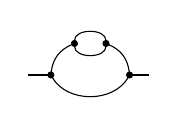
\begin{tikzpicture}[
    baseline={([yshift=-0.2cm]current bounding box.center)},
    scale=0.5,
    transform shape]
    \begin{feynman}
    % Vertici principali
    \vertex (a);
    \vertex [dot, right=0.5cm of a] (v1) {};
    \vertex [dot, right=2cm of v1] (v4) {};
    \vertex [dot, right=0.5cm of v4] (b);
    
    % Vertici per il loop superiore (posizionati manualmente sopra v1 e v4)
    \vertex [dot, above right=0.8cm and 0.6cm of v1] (v2) {};
    \vertex [dot, above left=0.8cm and 0.6cm of v4] (v3) {};

    \diagram* {
      (a) -- (v1),
      (v4) -- (b),
      % Arco inferiore del cerchio grande
      (v1) -- [bend right=60] (v4),
      % Pezzetti di arco superiore che portano alla bolla
      (v1) -- [bend left=30] (v2),
      (v3) -- [bend left=30] (v4),
      % La bolla superiore (il piccolo cerchio che interrompe)
      (v2) -- [bend left=90] (v3),
      (v2) -- [bend right=90] (v3),
    };
    \end{feynman}
    \end{tikzpicture}\bigg) = -4.
\end{equation}
\begin{obs}
    However, the diagram $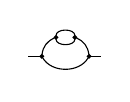
\begin{tikzpicture}[
    baseline={([yshift=-0.2cm]current bounding box.center)},
    scale=0.3,
    transform shape]
    \begin{feynman}
    % Vertici principali
    \vertex (a);
    \vertex [dot, right=0.5cm of a] (v1) {};
    \vertex [dot, right=2cm of v1] (v4) {};
    \vertex [dot, right=0.5cm of v4] (b);
    
    % Vertici per il loop superiore (posizionati manualmente sopra v1 e v4)
    \vertex [dot, above right=0.8cm and 0.6cm of v1] (v2) {};
    \vertex [dot, above left=0.8cm and 0.6cm of v4] (v3) {};

    \diagram* {
      (a) -- (v1),
      (v4) -- (b),
      % Arco inferiore del cerchio grande
      (v1) -- [bend right=60] (v4),
      % Pezzetti di arco superiore che portano alla bolla
      (v1) -- [bend left=30] (v2),
      (v3) -- [bend left=30] (v4),
      % La bolla superiore (il piccolo cerchio che interrompe)
      (v2) -- [bend left=90] (v3),
      (v2) -- [bend right=90] (v3),
    };
    \end{feynman}
    \end{tikzpicture}$ has 1-loop divergent sub-graph which is cancelled exactly by the counter-term insertion into the 1-loop diagram.
\end{obs}

This pattern continues to all-loop orders so the 1-loop counter-term is sufficient to render all correlation functions finite. There is one subtlety
\begin{equation}
    \omega(\feynmandiagram[inline={([yshift=-0.1cm]current bounding box.center)}, layered layout, horizontal=a to v, scale=0.5, transform shape] { 
        a -- v -- [half left, looseness=1.5] v1 -- [half left, looseness=1.5] v };) = 4 - 1 - 1 = 2,
\end{equation}
so the tadpole graph is also divergent 
\begin{equation}
    \begin{split}
        \feynmandiagram[inline={([yshift=-0.1cm]current bounding box.center)}, layered layout, horizontal=a to v, scale=0.5, transform shape] { a -- v -- [half left, looseness=1.5] v1 -- [half left, looseness=1.5] v }; &= -\frac{i\lambda_R\mu_R^\epsilon}{2}\int_k\frac{i}{D(k,m_R)} \\
        &= \frac{\lambda_R\mu_R^\epsilon}{2}I_1^{(1)[4 - 2\epsilon]} \\
        &= -\frac{i\lambda_R\Gamma(-1 + \epsilon)}{2\Gamma(1)}\frac{(m_R)^{1-\epsilon}}{(4\pi)^{2-\epsilon}} \mu_R^\epsilon \\
        &= \frac{i\lambda_R\mu_R^{-\epsilon}m_R^2}{2(4\pi)^2}\frac{\Gamma(1 + \epsilon)}{(-1 + \epsilon)\epsilon}\frac{1}{(4\pi)^{-\epsilon}}\bigg(\frac{\mu_R^2}{m_R^2}\bigg)^\epsilon \\
        &= \frac{i\lambda_R\mu_R^{-\epsilon}m_R^2}{2(4\pi)^2}\bigg[\frac{1}{\epsilon} + o(\epsilon^0)\bigg].
    \end{split}
\end{equation}
This graph contributes to the vacuum expectation value 
\begin{align}
    \mybrakett{0}{\phi}{0}_{free} &= 0, \\
    \mybrakett{0}{\phi}{0}_{int.} &= \mybrakett{0}{\phi S_{int}(\phi)}{0}_{free} + \cdots \\
    = \feynmandiagram[inline={([yshift=-0.1cm]current bounding box.center)}, layered layout, horizontal=a to v, scale=0.5, transform shape] { a -- v -- [half left, looseness=1.5] v1 -- [half left, looseness=1.5] v }; + \cdots.
\end{align}
The vacuum energy represents a physical observable and therefore we may renormalize the divergence into the vacuum 
\begin{equation}
    \mybrakett{0}{\phi}{0}_R = \vmedio{\phi}_P = \feynmandiagram[inline={([yshift=-0.1cm]current bounding box.center)}, layered layout, horizontal=a to v, scale=0.5, transform shape] { 
        a -- v -- [half left, looseness=1.5] v1 -- [half left, looseness=1.5] v}; + \feynmandiagram[inline={([yshift=-0.1cm]current bounding box.center)}, layered layout, horizontal=a to v, scale=0.9, transform shape] { 
        a -- v [crossed dot, pos=0.9]}; = 0 \\.
\end{equation}
The counter-term is introduced as a linear term is the Lagrangian in order to correct the quantum corrections exactly
\begin{equation}
    \dL = \frac{1}{2}\p_\mu\phi\p^\mu\phi - \frac{1}{2}m_R^2\phi^2 - \frac{\lambda_R\mu_R^\epsilon}{3!}\phi^3 + \frac{1}{2}\delta_{m}\phi^2 + \delta_{\vmedio{\phi}}\phi.
\end{equation}

\section{Alternative regularization methods}
Historically, dimensional regularization was introduced in 1972 mainly by 't Hooft and Veltmann. However, there are other options.

\paragraph{Cut-off regularization.} In this case we have
\begin{equation}
    \begin{split}
        \tadpole{2}{1}(\Delta) = \int_k^\Lambda \frac{1}{D(k,m)D(k - p,m)} &= \int_0^1 d\alpha\int_0^\Lambda \frac{d^4k}{(k^2 - \Delta)^2} \\
        &= i\int_0^1 d\alpha\int_0^\Lambda\frac{d|k_E||k_E|^3}{(k_E + \Delta)^2}\frac{2\pi^2}{(2\pi^4)} \\
        &= \frac{i}{16\pi^2}\int_0^1d\alpha\int_0^{\Lambda^2} dy\,\frac{y}{(y + \Delta)^2} \\
        &\simeq \frac{i}{16\pi^2}\int_0^1d\alpha\bigg[\log{\bigg(\frac{\Lambda^2}{\Delta}\bigg)} - 1\bigg].
    \end{split}
\end{equation}

\paragraph{Lattice regularization.} Discretising spacetime also regulates UV divergences. We keep gauge invariance but still break Poincaré invariance. If we write
\begin{equation}
    \selfint{D}(p^2,m^2) = \int_k\bigg(\frac{1}{D(k,m)D(k - p,m)} - \frac{1}{D(k,\mu)^2} + \frac{1}{D(k,\mu^2)}\bigg),
\end{equation}
by subtracting at fixed scale $\mu$ then the divergent integral 
\begin{equation}
    \int_k\frac{1}{D(k,\mu)^2} \propto \log{\bigg(\frac{1}{\mu^2a^2}\bigg)},
\end{equation}
where $x^\mu = n^\mu a$ with $a$ the lattice spacing and $-\pi/a \le k^\mu \le \pi/a$. 

\paragraph{Pauli-Villars regularization.} In this method we introduce new, large mass states such that the each propagator becomes
\begin{equation}
    \frac{1}{D(p,m)} \to \frac{1}{D(p,m)} + \frac{1}{D(p,M)} = \frac{m^2 - M^2}{D(p,m)D(p,M)},\quad M \gg m.
\end{equation}
The additional propagator factors enters the Feynman parameters and regulate the integrals but all expressions depend on $M$. 

\subsection{Analytic regularization}
We start from the observation that 
\begin{equation}
    \frac{\p}{\p p^2}\selfen{4}(p^2,m^2)
\end{equation}
is finite. From here we can begin to differentiate under the integral, so noting that 
\begin{equation}
    \frac{\p}{\p p^2} = \frac{p^\mu}{2p^2}\frac{\p}{\p p^\mu},\quad \frac{\p}{\p p^\mu}\frac{1}{D(k -p,m)} = \frac{(k - p)_\mu}{D(k - p,m)^2},
\end{equation}
we get
\begin{equation}
    \frac{\p}{\p p^2}\selfen{4}(p^2,m^2) = -\frac{i\lambda^2}{4p^2}\int \frac{d^4k}{(2\pi)^4}\frac{p(k - p)}{D(k,m)D(k - p,m)^2}.
\end{equation}
The additional powers of $k$ downstairs are sufficient to regulate the divergence in the UV. We can perform the Feynman parametrisation via
\begin{equation}
    \frac{1}{A^2B}  = 2\int_0^1 d\alpha\,\frac{\alpha}{[\alpha A + (1 - \alpha)B]^3},
\end{equation}
therefore
\begin{equation}
    \begin{split}
        \int_k\frac{p(k - p)}{D(k,m)D(k - p,m)^2} &= 2\int_0^1d\alpha\,\alpha\int_k\frac{p(k - p)}{[(k - \alpha p)^2 - \Delta]^3} \\
        &= 2\int_0^1d\alpha\,\alpha\int_k\frac{p(k + \alpha p - p)}{(k^2 - \Delta)^3}.
    \end{split}
\end{equation}
Now rewrite 
\begin{equation}
    \begin{split}
        \frac{\p}{\p p^2}\selfen{4}(p^2,m^2) &= -\frac{i\lambda^2}{2p^2}\int_0^1d\alpha\,\alpha\int_k\frac{kp - (1 - \alpha)p^2}{(k^2 - \Delta)^3} \\
        &= \frac{i\lambda^2}{2}\int_0^1d\alpha\,\alpha(1 - \alpha)\tadpole{3}{4}(\Delta) \\
        &= \frac{i\lambda^2}{2}\int_0^1d\alpha\,\alpha(1 - \alpha)\bigg(-\frac{i}{2\Delta(4\pi)^2}\bigg) \\
        &= -\frac{\lambda^2}{4(4\pi)^2}\frac{\p}{\p p^2}\int_0^1d\alpha\,\log{[-\alpha(1 - \alpha)p^2 + m^2]},
    \end{split}
\end{equation}
where we used the fact that
\begin{equation}
    \int_k\frac{kp}{(k^2 - \Delta)^n} = 0
\end{equation}
because the integrand is antisymmetric but the integration is done over a symmetric integration range. Therefore, we have
\begin{equation}
    \selfen{4}(p^2,m^2) = -\frac{\lambda^2}{4(4\pi)^2}\int_0^1d\alpha\,\alpha\log{(\Delta)} + C.
\end{equation}
We can now fix the constant using the renormalization scheme conditions, for example $\selfen{4}(p^2 = m^2) = 0$ in the on-shell scheme, in order to get
\begin{equation}
    \begin{split}
        \selfen{4}(p^2,m^2) &= -\frac{\lambda^2}{4(4\pi)^2}\bigg[\int_0^1d\alpha\,\log{(\Delta)} - \int_0^1d\alpha\,\log{(\Delta|_{p^2 = m^2})}\bigg] \\
        &= -\frac{\lambda^2}{4(4\pi)^2}\int_0^1d\alpha\,\log{\bigg(\frac{1 - \alpha(1 - \alpha)p^2/m^2}{1 - \alpha(1- \alpha)}\bigg)}
    \end{split}
\end{equation}

\section{Renormalization of \texorpdfstring{$\phi^3$}{phi3} in 6D at 1-loop}
In six dimensions the coupling constant $\lambda$ is dimensionless. The theory is renormalizable but in a more intricate way than in four dimensions. We start with the bare Lagrangian
\begin{equation}
    \dL = \frac{1}{2}\p_\mu\phi_0\p^\mu\phi_0 - \frac{1}{2}m_0^2\phi_0^2 - \frac{\lambda_0}{3!}\phi_0^3.
\end{equation}
The superficial degree of divergence is $\omega(\Gamma) = 6 - 2E$, so we have
\begin{equation}
    \omega(\feynmandiagram[inline={([yshift=-0.1cm]current bounding box.center)}, layered layout, horizontal=a to v, scale=0.5, transform shape] { a -- v -- [half left, looseness=1.5] v1 -- [half left, looseness=1.5] v };) = 4,\quad \omega(\feynmandiagram[inline={([yshift=-0.1cm]current bounding box.center)}, layered layout, horizontal=a to b, scale=0.5, transform shape] { a -- v -- [half left, looseness=1.5] v1 -- [half left, looseness=1.5] v, v1 -- b};) = 2,\quad \omega\bigg(\feynmandiagram [inline={([yshift=-0.1cm]current bounding box.center)}, scale = 0.5] { a -- [bend left=60] b -- [bend left=60] c -- [bend left=60] a, i1 -- a, i2 -- b,i3 -- c }; \bigg) = 0,
\end{equation}
and negative values for $E > 3$. This means we must also take care of divergences in the 3-point vertex function. Since $\omega$ is independent from the number of vertices $V$ the higher loop corrections to the 1-, 2- and 3-point functions also diverge, for example $\omega(\feynmandiagram [horizontal=v1 to v3, inline={([yshift=-0.1cm]current bounding box.center)}, scale=0.5] { a [dot] -- v1, v1 -- [quarter right, looseness=1.1] v2 [dot] -- [quarter right, looseness=1.1] v3 -- [quarter right, looseness=1.1] v4 [dot] -- [quarter right, looseness=1.1] v1, v3 -- b [dot], v2 -- v4, }; ) = 2$. We will first compute the divergent graphs and the show how they may be absorbed into a redefinition of the field and parameters in the Lagrangian. 

Computing directly using the bare Lagrangian, for the tadpole integral we have
\begin{equation}
    \begin{split}
        \feynmandiagram[inline={([yshift=-0.1cm]current bounding box.center)}, layered layout, horizontal=a to v, scale=0.5, transform shape] { a -- v -- [half left, looseness=1.5] v1 -- [half left, looseness=1.5] v }; &= -\frac{i\lambda_0}{2}i\tadpole{1}{6 - 2\epsilon}(m_0^2) \\
        &= -\frac{i\lambda}{2(4\pi)^{3 - \epsilon}}(m_0^2)^{2 - \epsilon}\frac{\Gamma(-2 + \epsilon)}{\Gamma(1)} \\
        &= -\frac{i\lambda_0}{2(4\pi)^3}\frac{(4\pi)^\epsilon\Gamma(1 + \epsilon)m_0^4(m_0^2)^{-\epsilon}}{\epsilon(1 - \epsilon)(2 - \epsilon)} \\
        &= -\frac{i\lambda_0m_0^4}{4(4\pi)^3}\bigg[\frac{1}{\epsilon} + \frac{3}{2} - \gamma_E + \log{(4\pi)} - \log{(m_0^2)}\bigg] + o(\epsilon);
    \end{split}
\end{equation}
for the bubble divergence we have
\begin{equation}
    \begin{split}
        \feynmandiagram[inline={([yshift=0cm]current bounding box.center)}, layered layout, horizontal=a to b, scale=0.5, transform shape] { a -- [momentum'={[arrow distance=3.5pt]\ensuremath{\scriptstyle p}}] v -- [half left, looseness=1.5] v1 -- [half left, looseness=1.5] v, v1 -- b}; &= \frac{(-i\lambda_0)^2}{2}\int_0^1d\alpha\,i^2\tadpole{2}{6 - 2\epsilon}\bigg[-\alpha(1 - \alpha)p^2 + m_0^2\bigg] \\
        &= \frac{i\lambda_0^2}{2(4\pi)^3}\bigg[\frac{1}{\epsilon}\bigg(-m_0^2 + \frac{p^2}{6}\bigg) + o(\epsilon^0)\bigg];
    \end{split}
\end{equation}
instead, for the triangular divergence we have
\begin{equation}
    \begin{split}
        \feynmandiagram[
        inline=(v1.base), horizontal=a to b, scale=0.8, transform shape] {
        a -- [reversed momentum'=\(\scriptstyle p_1\)] v1 -- [edge label=\( \alpha_3\), pos=0.5] v -- [edge label=\( \alpha_2\)] v2 -- [momentum'=\(\scriptstyle p_2\)] b, v1 -- [reversed momentum'=\(\scriptstyle k\), edge label'=\( \alpha_1\)] v2, v -- [momentum'=\(\scriptstyle p_3\)] c,
        }; &= (-i\lambda_0)^3\int_k\frac{i^3}{D(k,m)D(k-p,m)D(k-p_1-p_2,m)} \\
        &= \lambda_0^3\int_0^1d\alpha_1\int_0^{1-\alpha_1}d\alpha_2 \int_k\frac{2}{(k^2 - \Delta_3)^3} \\
        &= -2i\lambda_0^3\int_0^1 d\alpha_1\int_0^{1-\alpha_1} d\alpha_2\,\tadpole{3}{6 - 2\epsilon}(\Delta_3) \\
        &=(-i\lambda_0)(-i\lambda_0^2)\frac{2\Gamma(\epsilon)}{(4\pi)^{3 - \epsilon}\Gamma(3)}\int_0^1d\alpha_1\int_0^{1-\alpha_1}d\alpha_2\,\Delta_3^{-\epsilon},
    \end{split}
\end{equation}
where we defined
\begin{equation}
    \Delta_3 := m_0^2 - (1 - \alpha_1)\alpha_1p_1^2 - (1 - \alpha_2)\alpha_2p_2^2 - 2\alpha_1\alpha_2p_1p_2
\end{equation}
and used the relation
\begin{equation}
    \frac{1}{ABC} = \iiint\prod_{i=1}^3d\alpha_i\frac{2\delta(1 - \alpha_1 - \alpha_2 - \alpha_3)}{(\alpha_1A + \alpha_2B - \alpha_3C)^3}. 
\end{equation}
Expanding up to $o(\epsilon^0)$ is quite difficult in closed form, but keeping just $1/\epsilon$ is quite simple
\begin{equation}
    \feynmandiagram[
        inline=(v1.base), horizontal=a to b, scale=0.8, transform shape] {
        a -- [edge label=\(1\), pos=0.2] v1 -- v -- v2 -- [edge label=\(3\), pos=0.8] b, v1 -- v2, v -- [edge label=\(2\), pos=0.9] c,
        }; = \frac{(-i\lambda_0)\lambda_0^2}{2(4\pi)^3}\bigg[\frac{1}{\epsilon} + o(\epsilon^0)\bigg].
\end{equation}
The tadpole divergence is absorbed into the vacuum expectation value as in the $D = 4$ case, imposed by introducing a linear counter-term matching the tadpole graph
\begin{equation}
    \feynmandiagram[inline={([yshift=-0.1cm]current bounding box.center)}, layered layout, horizontal=a to v, scale=0.5, transform shape] { a -- v -- [half left, looseness=1.5] v1 -- [half left, looseness=1.5] v }; + \underbrace{\feynmandiagram[inline={([yshift=-0.1cm]current bounding box.center)}, layered layout, horizontal=a to v, scale=0.9, transform shape] { a -- v [crossed dot]};}_{\propto\,\delta_{\vmedio{\phi}}} = 0.
\end{equation}
The bubble divergence has changed it's functional form and is no longer absorbed by a simple mass shift. We saw
\begin{equation}
    \feynmandiagram[inline={([yshift=-0.1cm]current bounding box.center)}, layered layout, horizontal=a to b, scale=0.5, transform shape] { a -- v -- [half left, looseness=1.5] v1 -- [half left, looseness=1.5] v, v1 -- b}; \simeq \bigg(-m_0^2 + \frac{p^2}{6}\bigg)\frac{1}{\epsilon}.
\end{equation}
The first term can be obtained via a redefinition of the mass and a mass counter-term proportional to $\delta_{m}\phi^2$. The second term can be obtained from a redefinition of the field $\phi$ and the counter-term $(\p_\mu\phi\p^\mu\phi)\delta_\phi$ are called mass and wave function renormalization respectively. This can be written clearly introducing renormalization constants $Z_m$ and $Z_\phi$ defined as
\begin{equation}
    m_0^2 = Z_mm_R^2,\quad \phi_0 = \sqrt{Z_\phi}\phi_R,
\end{equation}
where $\delta_x = Z_x - 1$ for $x = \{m,\phi\}$. Applying this transformation to the Lagrangian leads to 
\begin{multline}
    \dL = \frac{1}{2}\p_\mu\phi_R\p^\mu\phi_R - \frac{1}{2}m_R^2\phi_R^2 + \dL_{int} + \\
    + \frac{1}{2}(1 - Z_\phi)\p_\mu\phi_R\p^\mu\phi_R - \frac{1}{2}(1 - Z_mZ_\phi)m_R^2\phi_R^2,
\end{multline}
from which we obtain a counter-term Feynman rule
\begin{equation}
    \feynmandiagram[inline={([yshift=-0.1cm]current bounding box.center)}, layered layout, horizontal=a to v, scale=0.9, transform shape] { a -- v [crossed dot] -- b}; = i(\delta_2p^2 - \delta_3m_R^2),\quad \delta_2 = \delta_\phi,\,\delta_3 = Z_mZ_\phi - 1.
\end{equation}
The renormalization constants can then be fixed at 1-loop via
\begin{equation}
    \feynmandiagram[inline={([yshift=-0.1cm]current bounding box.center)}, layered layout, horizontal=a to b, scale=0.5, transform shape] { a -- v -- [half left, looseness=1.5] v1 -- [half left, looseness=1.5] v, v1 -- b}; + \feynmandiagram[inline={([yshift=-0.25cm]current bounding box.center)}, layered layout, horizontal=a to v, scale=0.9, transform shape] { a -- v [crossed dot] -- [edge label=\ensuremath{\scriptstyle (1)}, pos=0.2] b }; = \mathrm{UV\,finite},\quad \forall p^2,m_R^2.
\end{equation}
The vertex divergence in the triangle function requires another counter-term that can be obtained through a redefinition of the coupling 
\begin{equation}
    \lambda_0 = Z_\lambda\lambda_R\mu_R^\epsilon,
\end{equation}
so that 
\begin{equation}
    \dL_{int} = \frac{\lambda_0\phi_0^3}{3!} = \frac{\lambda_R\mu_R^\epsilon}{3!}Z_\lambda Z_\phi^{3/2}\phi_R^3 \equiv \frac{\lambda_R\mu_R^\epsilon}{3!}Z_1\phi_R^3,
\end{equation}
where we defined $Z_1 := Z_\lambda Z_\phi^{3/2}$. This is charge renormalization and leads to a new counter-term with Feynman rule
\begin{equation}
    \feynmandiagram [inline={([yshift=-0.1cm]current bounding box.center)}, scale = 0.7] { a -- v[crossed dot], v -- b, v -- c }; = -i\lambda_R\mu^\epsilon_R\delta_1,
\end{equation}
which can be fixed at 1-loop using
\begin{equation}
    \feynmandiagram [inline={([yshift=-0.1cm]current bounding box.center)}, scale = 0.6, horizontal=v to v1] { a -- v, v -- v1, v1 -- v2, v2 -- v, v1 -- b, v2 -- c }; + \feynmandiagram [inline={([yshift=-0.1cm]current bounding box.center)}, scale = 0.7] { a -- [edge label=\ensuremath{\scriptstyle (1)}]  v [crossed dot], v -- b, v -- c }; = \mathrm{UV\,finite}.
\end{equation}
\begin{obs}
    We have $\delta_3 = \delta_m + \delta_\phi + \delta_n\delta_\phi$, where $\delta_\phi = \delta_2$, but the product term is always of higher order in perturbation theory than the linear terms so
    \begin{equation}
        \delta_m^{(1)} = \delta_3^{(1)} - \delta_\phi^{(1)},\quad \delta_m^{(2)} = \delta_3^{(2)} - \delta_\phi^{(2)} - \delta_3^{(1)}\delta_\phi^{(1)};
    \end{equation}
    we also have that $Z_1 = Z_\lambda Z_\phi^{3/2}$, therefore
    \begin{equation}
        \delta_\lambda^{(1)} = \delta_1^{(1)} - \frac{3}{2}\delta_\phi^{(1)}.
    \end{equation}
\end{obs}
We know have all the ingredients we need to complete the computation of the renormalization constants at 1-loop in the $\MMS$ scheme $\delta_\phi$, $\delta_m$ and $\delta_\lambda$; so from 
\begin{equation}
    \feynmandiagram[inline={([yshift=-0.1cm]current bounding box.center)}, layered layout, horizontal=a to b, scale=0.5, transform shape] { a -- v -- [half left, looseness=1.5] v1 -- [half left, looseness=1.5] v, v1 -- b}; + \feynmandiagram[inline={([yshift=-0.25cm]current bounding box.center)}, layered layout, horizontal=a to v, scale=0.9, transform shape] { a -- v [crossed dot] -- [edge label=\ensuremath{\scriptstyle (1)}, pos=0.2] b }; = \mathrm{UV\,finite}
\end{equation}
explicitly we get
\begin{equation}
    \frac{i\lambda_R^2\mu_R^{2\epsilon}}{2(4\pi)^3}\frac{(4\pi)^\epsilon\Gamma(1 + \epsilon)}{\epsilon}\bigg(-m_R^2 + \frac{p^2}{6}\bigg) + i(\delta_2^{(1)}p^2 - \delta_3^{(1)}m_R^2) = 0,
\end{equation}
therefore
\begin{align}
    \delta_2^{(1)} &= -\frac{\lambda_R^2\mu_R^{2\epsilon}}{2(4\pi)^3}\frac{r_\Gamma}{6\epsilon}, \\
    \delta_3^{(1)} &= -\frac{\lambda_R^2\mu_R^{2\epsilon}}{2(4\pi)^3}\frac{r_\Gamma}{\epsilon},
\end{align}
and from
\begin{equation}
    \feynmandiagram [inline={([yshift=-0.1cm]current bounding box.center)}, scale = 0.6, horizontal=v to v1] { a -- [edge label=\ensuremath{\scriptstyle 1}, pos=0.1] v, v -- v1, v1 -- v2, v2 -- v, v1 -- [edge label=\ensuremath{\scriptstyle 2}, pos=0.6] b, v2 -- [edge label=\ensuremath{\scriptstyle 3}, pos=0.9] c }; + \feynmandiagram [inline={([yshift=-0.1cm]current bounding box.center)}, scale = 0.7] { a -- [edge label=\ensuremath{\scriptstyle (1)}]  v [crossed dot], v -- b, v -- c }; = \mathrm{UV\,finite},
\end{equation}
we get
\begin{equation}
    (-i\lambda_R\mu_R^\epsilon)\frac{\lambda_R^2\mu_R^{2\epsilon}}{2(4\pi)^3}\frac{r_\Gamma}{\epsilon} + (-i\lambda_R\mu_R^\epsilon)\delta_1^{(1)} = 0,
\end{equation}
therefore
\begin{equation}
    \delta_1^{(1)} = -\frac{\lambda_R^2\mu_R^{2\epsilon}}{2(4\pi)^3}\frac{r_\Gamma}{\epsilon},
\end{equation}
where we defined 
\begin{equation}
    r_\Gamma := (4\pi)^\epsilon\Gamma(1 + \epsilon).
\end{equation}
Back in terms of $\delta_\phi^{(1)}$, $\delta_m^{(1)}$ and $\delta_\lambda^{(1)}$ we have
\begin{align}
    N_\lambda^{-1}\delta_1^{(1)} &= -\frac{1}{6\epsilon}, \\
    N_\lambda^{-1}\delta_m^{(1)} &= -\frac{1}{\epsilon} + \frac{1}{6\epsilon} = -\frac{5}{6\epsilon}, \\
    N_\lambda^{-1}\delta_\lambda^{(1)} &= -\frac{1}{\epsilon} -\frac{3}{2}\bigg(-\frac{1}{6\epsilon}\bigg) = -\frac{3}{4\epsilon},
\end{align}
where we defined 
\begin{equation}
    N_\lambda := \frac{\lambda_R^2\mu_R^{2\epsilon}r_\Gamma}{2(4\pi)^3}.
\end{equation}

\subsection{Other renormalization schemes}
For on-shell and momentum subtraction scheme we imposed a stricter condition that determined the finite terms. Since there are now three renormalization constants we must find an extended set of condition. These are
\begin{align}
    \lim_{p^2 \to x}\Gamma_{2,R}(p^2,m_R^2;\kappa_2,\kappa_3,\mu_R^2,\lambda_R^2) &= i\smallp, \\
    \lim_{p^2 \to x}\frac{\p\Gamma_{2,R}}{\p p^2}(p^2,m_R^2;\kappa_2,\kappa_3,\mu_R^2,\lambda_R^2) &= 1,
\end{align}
where $x = -M^2$ for the $\MOM$ scheme and $x = m_P^2 = m_R^2$ for the $\OS$ scheme. In $\MOM$ and $\MMS$ schemes we must also derive the relation between $m_R^2$ and $m_P^2$. For $\kappa$ we impose
\begin{equation}
    \lim_{p_i \to \substack{value\,where \\ \lambda_P\,measured}} G_{3,R}(p_1,p_2;\kappa_1,\mu_R^2,m_R^2,\lambda_R^2) = -\lambda_P
\end{equation}
for on the on-shell scheme and
\begin{equation}
    \lim_{p_i \to p_{sym}} G_{3,R}(p_1,p_2;\kappa_1,\mu_R^2,m_R^2,\lambda_R^2) = -\lambda_R
\end{equation}
for the $\MOM$ scheme where $p_{sym}$ is just the request that all the momenta are the same; in particular, the symmetric point is defined as
\begin{equation}
    p_i^2 = -\frac{2}{3}M^2\quad\Longrightarrow\quad p_i\cdot p_j = \frac{M^2}{3},\quad i \neq j.
\end{equation}

\subsection{Renormalization scale dependence}
Having fixed the three scheme constants $\kappa_i$ with the conditions on $\Gamma_{2}$, $\p_{p^2}\Gamma_2$ and $G_3$, we have determined $m_R$ and $\lambda_R$ in terms of some fixed values (physical measurements) $m_P$ and $\lambda_P$ but the dependence on $\mu_R^2$ remains. This is a feature of the re-organized, renormalized perturbative series. Eventually, it must be that the dependences go away as we scan to all the orders. The Lagrangian after all has not changed
\begin{equation}
    \dL(\phi_0,m_0,\lambda_0) = \dL(\phi_R,m_R,\lambda_R;\mu_R),
\end{equation}
which means the bare correlation functions do not depend on $\mu_R$
\begin{equation}
    \begin{split}
        \tilde{G}_0(p_1,\dots,p_n;\lambda_0) &= FT(\mybrakett{0}{T\{\phi_0(x_1)\cdots\phi_0(x_n)\}}{0}) \\
        &= Z_\phi^{n/2}(\mu_R,\lambda_R(\mu_R))FT(\mybrakett{0}{T\{\phi_R(x_1)\cdots\phi_R(x_n)\}}) \\
        &= Z_\phi^{n/2}(\mu_R,\lambda_R(\mu_R))\tilde{G}_R(p_1,\dots,p_n;\lambda_R(\mu_R),\mu_R).
    \end{split}
\end{equation}
So the $\mu_R$ dependence of $\tilde{G}$ must cancel exactly with the $\mu_R$ dependence of $Z_\phi^{3/2}$. In other words
\begin{equation}
    \frac{\p\tilde{G}_0}{\p\mu_R} = \frac{\p}{\p\mu_R}(Z_\phi^{n/2}\tilde{G}_R) = Z_\phi^{n/2}\frac{\p}{\p\mu_R}(\tilde{G}_R) + \tilde{G}_R\frac{\p}{\p\mu_R}(Z_\phi^{n/2}) = 0,
\end{equation}
whose consequences are going to be discussed later on.


% \chapter{Loop integration methods}
In this chapter will expand on the techniques used in the previous chapter and develop methods read to continue our discussion to gauge theories. We came across three examples of Feynman parametrisation
\begin{align}
    \frac{1}{AB} &= \int_0^1 d\alpha\frac{1}{[A\alpha + B(1 - \alpha)]^2}, \\
    \frac{1}{AB^2} &= 2\int_0^1 d\alpha\,\frac{\alpha}{[A\alpha + B(1 - \alpha)]^2}, \\
    \frac{1}{ABC} &= 2\int_0^1 d\alpha_1\int_0^{1 - \alpha_1}d\alpha_2\frac{1}{[A\alpha_1 + B\alpha_2 + C(1 - \alpha_1 - \alpha_2)]^3},
\end{align}
but the general version is
\begin{equation}
    \frac{1}{\prod_{i=1}^nA_i^{\nu_i}} = \frac{\Gamma(\sum_{i=1}^n\nu_i)}{\prod_{i=1}^n\Gamma(\nu_i)}\int_0^1\prod_{i=1}^nd\alpha_i\,\frac{\alpha_i^{\nu_i - 1}\delta(1 - \sum_{i=1}^n\alpha_i)}{(\sum_{i=1}^nA_i\alpha_i)^{\sum_{i=1}^n\nu_i}}.
\end{equation}
A similar transformation is provided through Schwinger parameters
\begin{equation}
    \frac{1}{D^\nu} = \frac{(-1)^\nu}{\Gamma(\nu)}\int_0^\infty dt\,t^{\nu - 1}\exp{(tD)}.
\end{equation}
The 1-loop bubble example becomes
\begin{equation}
    \begin{split}
        \selfint{D} &= \int_k\int_0^\infty dt_1\int_0^\infty dt_2\,\exp{[t_1D(k,m) + t_2D(k - p,m)]} \\
        &= \int_k\int_{t_i}\exp{\bigg[(t_1 + t_2)(k^2 - m^2) + \frac{t_1t_2}{t_1 + t_2}p^2\bigg]} \\
        &= \int_k\int_{t_i}\exp{(ak^2 - b)},
    \end{split} 
\end{equation}
where we performed the shift 
\begin{equation}
\label{eq: loop momentum shift}
    k \to k + \frac{t_2p}{t_1 + t_2}
\end{equation}
and imposed
\begin{equation}
    a \equiv t_1 + t_2,\quad b \equiv m^2(t_1 + t_2) - \frac{t_1t_2}{t_1 + t_2}p^2,\quad \int_{t_i} \equiv \int_0^\infty dt_1\int_0^\infty dt_2.
\end{equation}
The integral over $k$ can be performed after a Wick rotation 
\begin{equation}
    \begin{split}
        \selfint{D} &= i\int_{t_i}\int_{k_E}\exp{(-ak_E^2)}\exp{(-b)} \\
        &= \frac{i}{(4\pi)^{D/2}}\int_{t_i}\exp{(-b)}a^{-D/2}.
    \end{split}
\end{equation}

\section{Tensor integrals}
When considering gauge theories we will find loop momentum dependent numerators which require further analysis. We did find one case already in the case of $\p\Sigma/\p p^2$ for $\phi^3$ theory although it was handled in an easy manner. Let's try the example again using Schwinger parameters
\begin{equation}
    \selfint{D}[k^\mu] = \int_k\frac{k^\mu}{D(k,m)D(k - p,m)}.
\end{equation}
The loop momentum shift \eqref{eq: loop momentum shift} that we used to put the denominator in standard form also affects the numerator, so
\begin{equation}
    \begin{split}
        \selfint{D}[k^\mu] &= \int_k\int_{t_i}\bigg[k + \frac{t_2p}{(t_1 + t_2)}\bigg]\exp{(ak^2 - b)} \\
        &= p^\mu\int_{t_i}\frac{t_2}{(t_1 + t_2)}\frac{i}{(4\pi)^{D/2}}a^{-D/2}\exp{(-b)},
    \end{split}
\end{equation}
where we have used that $\int_k k^\mu\exp{(ak^2)} = 0$. The parametric integration seems more difficult but we can use the symmetry with respect to the swap of $t_1$ and $t_2$ to write
\begin{equation}
    \begin{split}
        \selfint{D}[k^\mu] &= \frac{p^\mu}{2}\int_{t_i}\bigg(\frac{t_1}{t_1 + t_2} + \frac{t_2}{t_1 + t_2}\bigg)\frac{i}{(4\pi)^{D/2}}a^{-D/2}\exp{(-b)} \\
        &= \frac{p^\mu}{2}\selfint{D}.
    \end{split}
\end{equation}
The tensor rank of a Feynman integral is the total power of all loop momenta in the numerator of the integrand. As we increase the tensor rank we encounter new loop momentum integrals, we can distinguish:
\begin{enumerate}
    \item if the rank is odd then the integral evaluates at
    \begin{equation}
    \label{eq: odd rank Feynman integrals}
        \int_k k^{\mu_1}\cdots k^{\mu_{2n + 1}} \exp{(ak^2)} = 0,\quad n \in \Z;
    \end{equation}
    \item if the rank is even then the integral evaluates at
    \begin{equation}
    \label{eq: even rank Feynman integrals}
        \int_k k^{\mu_1}\cdots k^{\mu_{2n}} \exp{(ak^2)} = -\frac{1}{2a}\sum_{i=2}^{2n}g^{\mu_1\mu_i}\int_k\frac{k^{\mu_1}\cdots k^{\mu_{2n}}}{k^{\mu_1}k^{\mu_i}},\quad n \in \Z.
    \end{equation}
\end{enumerate}
In particular, we denote
\begin{equation}
    K \equiv \int_k\exp{(ak^2)} = \frac{i}{(4\pi)^{D/2}}e^{-D/2},
\end{equation}
so the first two integrals, other than $K$, are
\begin{align}
    \int_k k^\mu \exp{(ak^2)} &= 0,\quad 
    \int_k k^\mu k^\nu \exp{(ak^2)} = -\frac{1}{2a}g^{\mu\nu}K.
\end{align}
\begin{obs}
    Let's prove the rank two case of \eqref{eq: even rank Feynman integrals} given by
    \begin{equation}
        \int_k k^\mu k^\nu\exp{(ak^2)} = Ag^{\mu\nu},
    \end{equation}
    where $A$ is the unknown form factor. We begin by contracting both sides with the metric $g^{\mu\nu}$ remembering that $g^{\mu\nu}g_{\mu\nu} = D$, thus from
    \begin{equation}
        \begin{split}
            \int_k k^2\exp{(ak^2)} = AD &= \int_k\frac{\p}{\p a}\exp{(ak^2)} \\
            &= \frac{\p}{\p a}\int_k\exp{(ak^2)} \\
            &= \frac{\p}{\p a}\bigg[\frac{i}{(4\pi)^{D/2}}e^{-D/2}\bigg] \\
            &= -\frac{D}{2a}\frac{i}{(4\pi)^{D/2}}e^{-D/2},
        \end{split}
    \end{equation}
    we get, comparing the first step with the last one, the expected result
    \begin{equation}
        A = -\frac{1}{2a}K.
    \end{equation}
\end{obs}
Similar expressions are obtained using Feynman parameters after following the same steps, for example
\begin{align}
    \begin{split}
        \selfint{D}[k^\mu] &= \int_0^1 d\alpha\int_k \frac{k^\mu + \alpha p^\mu}{(k^2 - \Delta)^2} \\
        &= p^\mu\int_0^1 d\alpha\,\alpha\tadpole{2}{D}(\Delta),
    \end{split} \\
    \begin{split}
        \selfint{D}[k^\mu,k^\nu] &= \int_0^1 d\alpha\int_k \frac{(k^\mu + \alpha p^\mu)(k^\nu + \alpha p^\nu)}{(k^2 - \Delta)^2} \\
        &= p^\mu p^\nu\int_0^1 d\alpha\,\alpha^2\tadpole{2}{D}(\Delta) \\
        &+ \frac{g^{\mu\nu}}{D}\int_0^1 d\alpha\,[\tadpole{1}{D}(\Delta) + \Delta\tadpole{2}{D}(\Delta)].
    \end{split}
\end{align}

\subsection{Multi-loop parametrisations}
It is possible to find a general parametrisation for any multi-loop graph in which we can perform the integration in $k_i^\mu$ but leave integrals over the Feynman or the Schwinger parameters. Let's consider a 2-loop graph with $n$ denominators defined through 
\begin{align}
    D_i &= D(q_i,m_i) = q_i^2 - m_i^2, \\
    q_i &= \lambda_{ij}k_j^\mu + \sigma_{il}p_e^\mu,
\end{align}
where $k_j^\mu$ with $j = \{1,2\}$ are the loop momenta and $p_e^\mu$ are the independent external momentum
\begin{equation}
    \selfint{D} = \int_{k_1}\int_{k_2}\frac{1}{\prod_{i=1}^nD_i}.
\end{equation}
The combined arguments at the exponential after introducing Schwinger parameters $x_i$ for each $D_i$ is $\sum_{i=1}^nx_iD_i$ which we may decompose according to the loop momentum structures
\begin{equation}
    \sum_{i=1}^n x_iD_i = k_{i\mu}M_{ij}k_j^\mu + 2k_{i\mu}Q_i^\mu + J,
\end{equation}
where:
\begin{enumerate}
    \item $M$ is a symmetric $2\times 2$ matrix depending on $x_i$;
    \item $Q_i^\mu$ is a vector linear in $p_e^\mu$ with coefficient dependent on $x_i$;
    \item $J$ is a scalar quantity depending on momentum invariants and $x_i$.
\end{enumerate}
Thus, the relation can be written as
\begin{equation}
\label{eq: argument of exponential with S. parameters}
    \sum_{i=1}^n x_iD_i = k^TMk + 2k^T\vQ + J.
\end{equation}
As a concrete example we can take a look at a 2-loop propagator graph
\begin{equation}
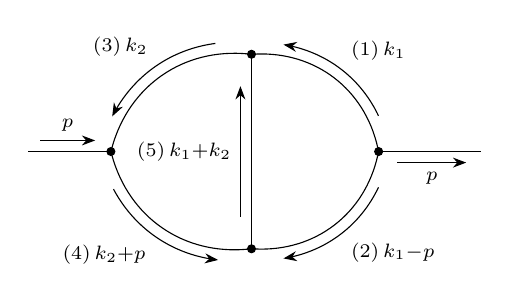
\begin{tikzpicture}   
\begin{feynman}[inline={([yshift=-0.1cm]current bounding box.center)}, scale=1, transform shape]
    % Vertici principali
    \vertex (a);
    \vertex [dot, right=1cm of a] (v1) {};
    \vertex [dot, right=3.4cm of v1] (v2) {};
    \vertex [dot, right=1.3cm of v2] (b);
    \vertex [dot, below right=1.2cm and 2.8cm of a] (down) {};
    \vertex [dot, above right=1.2cm and 2.8cm of a] (up) {};

    \diagram* {
      (a) -- [momentum={[arrow distance = 4pt]\(\scriptstyle p\)}] (v1),
      (v1) -- [bend right=40, momentum'={[arrow distance = 4pt]\(\scriptstyle (4)\, k_2 + p\)}] (down), (down) -- [bend right=40, reversed momentum'={[arrow distance = 4pt]\(\scriptstyle (2)\, k_1 - p\)}] (v2),
      (v2) -- [bend right=40, momentum'={[arrow distance = 4pt]\(\scriptstyle (1)\,k_1\)}] (up), (up) -- [bend right=40, momentum'={[arrow distance = 4pt]\(\scriptstyle (3)\, k_2\)}] (v1), (v2) -- [momentum'={[arrow distance = 4pt]\(\scriptstyle p\)}] (b), (down) -- [momentum={[arrow distance = 4pt]\(\scriptstyle (5)\, k_1 + k_2\)}]  (up)
    };
  \end{feynman}
\end{tikzpicture}
\end{equation}
The matrix $M$ can be written simply following the propagator dependence on each Schwinger parameter
\begin{equation}
    M = 
    \begin{pmatrix}
        x_1 + x_2 + x_5 & x_5 \\
        x_5 & x_3 + x_4 + x_5
    \end{pmatrix},
\end{equation}
linear dependence of $k_1$ and $k_2$ comes only from propagators ``2'' and ``4'' so
\begin{equation}
    Q^\mu = \{-p^\mu x_2, p^\mu x_4\},
\end{equation}
and $J$ contains all mass dependence and $p^2$ terms 
\begin{equation}
    J = -\bigg(\sum_{i=1}^5 x_i\bigg)m^2 + (x_2 + x_4)p^2.
\end{equation}
From the general form \eqref{eq: argument of exponential with S. parameters} we can ``complete the square'' in $k$ which we do in two stages: diagonalize $M$ and then shift using $Q$. Firstly, consider a general symmetric $2 \times 2$ matrix
\begin{equation}
    M = 
    \begin{pmatrix}
        a & c \\
        c & b
    \end{pmatrix},
\end{equation}
completing the square in $k$, can be performed via transformation with unit determinant
\begin{equation}
    \Lambda = 
    \begin{pmatrix}
        1 & -c/a \\
        0 & 1
    \end{pmatrix},
\end{equation}
where with $\vk = (k_1,k_2)$ we have $\vk = \Lambda \vk'$, thus
\begin{equation}
    \vk^TM\vk = (\Lambda\vk')^TM\Lambda\vk' = \vk'^T(\Lambda^TM\Lambda)\vk'\equiv \vk'^TD\vk',
\end{equation}
where we denoted
\begin{equation}
    D \equiv 
    \begin{pmatrix}
        a & 0 \\
        0 & \dfrac{\det{(M)}}{a}
    \end{pmatrix}.
\end{equation}
The second step consists in absorbing the linear terms in linear $k_i$ via a transformation 
\begin{equation}
    \vk' = \vk'' - \Lambda^{-1}M^{-1}\vQ,
\end{equation}
therefore
\begin{equation}
    \begin{split}
        \vk'^TD\vk' + 2\vQ^T\Lambda\vk' + J &= \vk''^TD\vk'' - \vk''^TD\Lambda^{-1}M^{-1}\vQ \\
        &- (\Lambda^{-1}M^{-1}\vQ)^TD\vk'' + (\Lambda^{-1}M^{-1}\vQ)^TD\Lambda^{-1}M^{-1}\vQ \\
        &+ 2\vQ^T\Lambda\vk'' - 2\vQ^T\Lambda\Lambda^{-1}M^{-1}\vQ + J \\
        &= \vk''^TD\vk'' + J - \vQ^TM^{-1}\vQ.
    \end{split}
\end{equation}
Both steps can be combined so that
\begin{equation}
    \vk'' = \Lambda\vk - M^{-1}\vQ 
\end{equation}
and the argument of the exponential is written as
\begin{equation}
    \sum_{i=1}^nx_iD_i = \vk^TD\vk + \frac{F}{u},
\end{equation}
where we denoted
\begin{equation}
    u \equiv \det{M},\quad F \equiv (J - \vQ^TM^{-1}\vQ)u,
\end{equation}
which are the first two of the Symanzik polynomials and permit to write
\begin{equation}
    D = 
    \begin{pmatrix}
        a & 0 \\
        0 & \dfrac{u}{a}
    \end{pmatrix}.
\end{equation}
The transformation has separated the loop integrals so we can perform the integration
\begin{equation}
    \begin{split}
        \selfint{D} &= \int\prod_{i=1}^n dx_i\,\exp{\bigg(\frac{F}{u}\bigg)} \int_{k_1}\exp{(ak_1^2)}\int_{k_2}\exp{\bigg(\frac{uk_2^2}{a}\bigg)} \\
        &= \bigg[\frac{i}{(4\pi)^{D/2}}\bigg]^2\int\prod_{i=1}^n dx_i\,\exp{\bigg(\frac{F}{u}\bigg)}u^{-D/2}.
    \end{split}
\end{equation}
By following the same procedure we can derive a general multi-loop expression valid for arbitrary powers of the determinants. One can show that a general $L$-loop Feynman integral with $n$ interval lines may be written as
\begin{equation}
    \begin{split}
        I_{n,sun}^{(L)[D]}[\nu_1,\dots,\nu_n] &= \int\prod_{i=1}^L\frac{d^Dk_l}{(2\pi)^D}\frac{1}{\prod_{j=1}^nD(q_j,m_j)^{\nu_j}} \\
        &= \bigg[\frac{i}{(4\pi)^{D/2}}\bigg]^L\frac{\Gamma(\sum_{i=1}^n\nu_i - LD/2)}{\prod_{i=1}^n\Gamma(\nu_i)} \\
        &\times\int_{\alpha_i}\delta(1 - \nsum_i\alpha_i)\frac{u^{n-(L+1)D/2}}{(-F)^{n-LD/2}},
    \end{split} 
\end{equation}
where $u$ and $F$ are the Symanzik polynomials. 
\begin{ex}
    The ``sunrise'', or the ``sunset'', integral is
    \begin{equation}
        \feynmandiagram[inline={([yshift=-0.1cm]current bounding box.center)}, layered layout, horizontal=a to b, scale=1.8] { a -- [momentum={[arrow distance=4pt]\ensuremath{\scriptstyle p}}] v [dot] -- [half left, looseness=1.5, momentum={[arrow distance=4pt]\ensuremath{\scriptstyle k_1}}] v1 [dot] -- [half left, looseness=1.5, reversed momentum={[arrow distance=4pt]\ensuremath{\scriptstyle k_2}}] v, v1 -- [momentum={[arrow distance=4pt]\ensuremath{\scriptstyle p}}] b, v -- [reversed momentum={[arrow distance = 4pt]\ensuremath{\scriptstyle k_1 + k_2 - p}}] v1};.
    \end{equation}
    From this diagram here we get
    \begin{equation}
        M = 
        \begin{pmatrix}
            x_1 + x_3 & x_3 \\
            x_3 & x_2 + x_3
        \end{pmatrix},\quad \vQ = (-x_3p^\mu,-x_3p^\mu),\quad J = x_3p^2,
    \end{equation}
    from where we get
    \begin{equation}
        u = x_1x_2 + x_1x_3 + x_2x_3,\quad F = p^2x_1x_2x_3.
    \end{equation}
    Thus, the Feynman integral is
    \begin{equation}
        \begin{split}
            I_{n,sun}^{(L)[D]} &= \frac{\Gamma(-1 + 2\epsilon)}{(4\pi)^{4 - 2\epsilon}}\int\prod_{i=1}^3 dx_i\,\delta(1 - x_1 - x_2 - x_3) \\
            &\times(-p^2x_1x_2x_3)^{1 - 2\epsilon}(x_1x_2 + x_1x_3 + x_2x_3)^{-3(1 - \epsilon)}.
        \end{split}
    \end{equation}
    Direct integration in Fourier phase space requires a bit of thought. The $1/\epsilon$ pole is quite easy since we may expand the integral around $\epsilon = 0$. The kinematic dependence can also factored out
    \begin{equation}
        I_{n,sun}^{(L)[D]} = \bigg[\frac{C_\Gamma}{(4\pi)^{2-\epsilon}}\bigg]^2(-p^2)^{1-2\epsilon}\hat{I}_{n,sun}^{(L)[D]}[\nu_1,\dots,\nu_n],
    \end{equation}
    where
    \begin{equation}
        \begin{split}
            \hat{I}_{n,sun}^{(L)[D]} &= -\frac{\Gamma(1 + 2\epsilon)}{2\epsilon(1-2\epsilon)C_\Gamma^2}\int_{x_i}\delta\bigg(1 - \sum_{i=1}^nx_i\bigg)(x_1x_2x_3)^{1-2\epsilon} \\
            &\times (x_1x_2 + x_1x_3 + x_2x_3)^{-3(1 - \epsilon)} \\
            &\simeq -\frac{1}{4\epsilon} - \frac{13}{8} - \frac{115}{16}\epsilon - \bigg(\frac{865}{32} - \frac{3\zeta_3}{2}\bigg)\epsilon^2 \\
            &-\bigg(\frac{5971}{64} - \frac{39}{4}\zeta_3 - \frac{\pi^4}{40}\bigg)\epsilon^3 + o(\epsilon^4).
        \end{split}
    \end{equation}
\end{ex}

\subsection{Passarino-Veltmann tensor reduction}
We have already seen how to deal with higher rank numerators in Feynman or Schwinger parameter space. There is a more direct method to perform the reduction in momentum space and to determine the basis of Feynman integrals at 1-loop. The principles are:
\begin{enumerate}
    \item identify a basis of possible tensor structures after integration using the external momentum $p_i^\mu$ and the metric tensor $g^{\mu\nu}$;
    \item contract the tensor integral in $D$ dimensions with each element of the tensor basis to construct a linear system of equations for the form factors, namely the coefficient of the tensor basis.
\end{enumerate}
\begin{ex}
    Consider the rank one bubble
    \begin{equation}
        \selfint{D}[k^\mu] = \int_k\frac{k^\mu}{D(k,m)D(k - p,m)}.
    \end{equation}
    The first step is to impose $\selfint{D} = b_1p^\mu$, where $b_1$ is the form factor and $p^\mu$ is the tensor basis, then we contract with $p_\mu$ so that
    \begin{equation}
        \begin{split}
            \selfint{D}[p_\mu k^\mu] = b_1p^2 &= \int_k \frac{p_\mu k^\mu}{D(k,m)D(k - p,m)} \\
            &= \frac{1}{2}\int \frac{D(k,m) - D(k - p,m) + p^2}{D(k,m)D(k - p,m)} \\
            &= \frac{1}{2}\bigg(\int_k \frac{1}{D(k - p,m)} - \int_k \frac{1}{D(k,m)} \\
            &+ p^2\int_k \frac{1}{D(k,m)D(k - p,m)}\bigg) \\
            &= \frac{1}{2}p^2\selfint{D}[1],
        \end{split}
    \end{equation}
    where in the second-last step we shifted the integration $k \to k + p$ in the first integral to cancel it out with the last integral. Thus, the form factor is
    \begin{equation}
        b_1 = \frac{1}{2}\selfint{D}[1].
    \end{equation}
    We can also write this graphically
    \begin{equation}
        \feynmandiagram[inline={([yshift=-0.3cm]current bounding box.center)}, layered layout, horizontal=a to b, scale=0.5, transform shape] { a -- v -- [half left, looseness=1.5, momentum={[arrow distance=3pt] \ensuremath{\scriptstyle k}}] v1 -- [half left, looseness=1.5] v, v1 -- b};[k^\mu] = \selfint{D}[k^\mu],
    \end{equation}
    then
    \begin{equation}
        \begin{split}
            \feynmandiagram[inline={([yshift=-0.1cm]current bounding box.center)}, layered layout, horizontal=a to b, scale=0.5, transform shape] { a -- v -- [half left, looseness=1.5, momentum={[arrow distance=3pt] \ensuremath{\scriptstyle k}}] v1 -- [half left, looseness=1.5, momentum={[arrow distance=3pt] \ensuremath{\scriptstyle k - p}}] v, v1 -- b};[p_\mu k^\mu] &= \frac{1}{2}\feynmandiagram[inline={([yshift=-0.1cm]current bounding box.center)}, layered layout, horizontal=a to b, scale=0.5, transform shape] { a -- v -- [half left, looseness=1.5, cancel] v1 -- [half left, looseness=1.5] v, v1 -- b};[1] - \frac{1}{2}\feynmandiagram[inline={([yshift=-0.1cm]current bounding box.center)}, layered layout, horizontal=a to b, scale=0.5, transform shape] { a -- v -- [half left, looseness=1.5] v1 -- [half left, looseness=1.5, cancel] v, v1 -- b};[1] + \frac{p^2}{2}\feynmandiagram[inline={([yshift=-0.1cm]current bounding box.center)}, layered layout, horizontal=a to b, scale=0.5, transform shape] { a -- v -- [half left, looseness=1.5] v1 -- [half left, looseness=1.5] v, v1 -- b};[1] \\
            &= b_1p^2,
        \end{split}
    \end{equation}
    where $\feynmandiagram[inline={([yshift=-0.1cm]current bounding box.center)}, horizontal=a to b, scale=0.7]{
    a -- [cancel] b}; $ indicates a canceled propagator. Thus we have
    \begin{equation}
        \begin{cases}
            \feynmandiagram[inline={([yshift=-0.1cm]current bounding box.center)}, layered layout, horizontal=a to b, scale=0.5, transform shape] { a -- v -- [half left, looseness=1.5, cancel] v1 -- [half left, looseness=1.5] v, v1 -- b};[1] = \feynmandiagram[inline={([yshift=0.4cm]current bounding box.center)}, layered layout, horizontal=a to b, scale=0.5, transform shape] { a -- v -- [out=-135, in=-45, loop, min distance=1.4cm, reversed momentum'={[arrow distance=4pt] \ensuremath{\scriptstyle k - p}}] v -- b };[1] = \feynmandiagram[inline={([yshift=-0.5cm]current bounding box.center)}, layered layout, horizontal=a to b, scale=0.5, transform shape] { a -- v -- [out=135, in=45, loop, min distance=1.4cm, momentum={[arrow distance=4pt] \ensuremath{\scriptstyle k}}] v -- b };[1] \\
            \feynmandiagram[inline={([yshift=-0.1cm]current bounding box.center)}, layered layout, horizontal=a to b, scale=0.5, transform shape] { a -- v -- [half left, looseness=1.5] v1 -- [half left, looseness=1.5, cancel] v, v1 -- b};[1] = \feynmandiagram[inline={([yshift=-0.5cm]current bounding box.center)}, layered layout, horizontal=a to b, scale=0.5, transform shape] { a -- v -- [out=135, in=45, loop, min distance=1.4cm, momentum={[arrow distance=4pt] \ensuremath{\scriptstyle k}}] v -- b };[1]
        \end{cases},
    \end{equation}
    so the form factor is
    \begin{equation}
        b_1 = \frac{1}{2}\feynmandiagram[inline={([yshift=-0.1cm]current bounding box.center)}, layered layout, horizontal=a to b, scale=0.5, transform shape] { a -- v -- [half left, looseness=1.5] v1 -- [half left, looseness=1.5] v, v1 -- b};[1].
    \end{equation}
\end{ex}
The principle is straightforward to apply to higher rank and higher multiplicity integrals though the expressions can become quite lengthy. 
\begin{ex}
    Consider the rank two tensor bubble
    \begin{equation}
        \feynmandiagram[inline={([yshift=-0.3cm]current bounding box.center)}, layered layout, horizontal=a to b, scale=0.5, transform shape] { a -- [momentum={[arrow distance=4pt] \ensuremath{\scriptstyle p}}] v -- [half left, looseness=1.5, momentum={[arrow distance=4pt] \ensuremath{\scriptstyle k}}] v1 -- [half left, looseness=1.5] v, v1 -- b};[k^\mu k^\nu] = b_{00}g^{\mu\nu} + b_{11}p^\mu p^\nu,
    \end{equation}
    now contracting with $g_{\mu\nu}$ we get
    \begin{equation}
        \begin{split}
            \feynmandiagram[inline={([yshift=-0.3cm]current bounding box.center)}, layered layout, horizontal=a to b, scale=0.5, transform shape] { a -- v -- [half left, looseness=1.5, momentum={[arrow distance=4pt] \ensuremath{\scriptstyle k}}] v1 -- [half left, looseness=1.5] v, v1 -- b};[k^2] &= Db_{00} + b_{11}p^2 \\
            &= \feynmandiagram[inline={([yshift=-0.1cm]current bounding box.center)}, layered layout, horizontal=a to b, scale=0.5, transform shape] { a -- v -- [half left, looseness=1.5, cancel] v1 -- [half left, looseness=1.5] v, v1 -- b};[1] + m^2\feynmandiagram[inline={([yshift=-0.1cm]current bounding box.center)}, layered layout, horizontal=a to b, scale=0.5, transform shape] { a -- v -- [half left, looseness=1.5] v1 -- [half left, looseness=1.5] v, v1 -- b};[1] \\
            &=  \feynmandiagram[inline={([yshift=0.1cm]current bounding box.center)}, layered layout, horizontal=a to b, scale=0.5, transform shape] { a -- v -- [out=-135, in=-45, loop, min distance=1.4cm] v -- b };[1] + m^2\feynmandiagram[inline={([yshift=-0.1cm]current bounding box.center)}, layered layout, horizontal=a to b, scale=0.5, transform shape] { a -- v -- [half left, looseness=1.5] v1 -- [half left, looseness=1.5] v, v1 -- b};[1],
        \end{split}
    \end{equation}
    while contracting with $p_\mu p_\nu$ result in
    \begin{equation}
        \begin{split}
            \feynmandiagram[inline={([yshift=-0.3cm]current bounding box.center)}, layered layout, horizontal=a to b, scale=0.5, transform shape] { a -- v -- [half left, looseness=1.5, momentum={[arrow distance=4pt] \ensuremath{\scriptstyle k}}] v1 -- [half left, looseness=1.5] v, v1 -- b};[(p_\mu k^\mu)^2] &= b_{00}p^2 + b_{11}p^4 \\
            &= \feynmandiagram[inline={([yshift=-0.3cm]current bounding box.center)}, layered layout, horizontal=a to b, scale=0.4, transform shape] { a -- v -- [half left, looseness=1.5, momentum={[arrow distance=4pt] \ensuremath{\scriptstyle k}}] v1 -- [half left, looseness=1.5] v, v1 -- b};\bigg[\frac{1}{2}\bigg(D(k,m) - D(k - p,m) + p^2\bigg)^2\bigg] \\
            &= \frac{1}{4}\feynmandiagram[inline={([yshift=-0.3cm]current bounding box.center)}, layered layout, horizontal=a to b, scale=0.4, transform shape] { a -- v -- [half left, looseness=1.5, momentum={[arrow distance=4pt] \ensuremath{\scriptstyle k}}] v1 -- [half left, looseness=1.5] v, v1 -- b};\{D(k,m)^2 + D(k - p,m)^2  \\ &- 2D(k,m)D(k - p,m) + p^4 + 2p^2[D(k,m) \\
            &- D(k - p,m)]\} \\
            &= \frac{1}{4}(p^4\feynmandiagram[inline={([yshift=-0.1cm]current bounding box.center)}, layered layout, horizontal=a to b, scale=0.4, transform shape] { a -- v -- [half left, looseness=1.5] v1 -- [half left, looseness=1.5] v, v1 -- b};[1] + \feynmandiagram[inline={([yshift=-0.1cm]current bounding box.center)}, layered layout, horizontal=a to b, scale=0.4, transform shape] { a -- v -- [half left, looseness=1.5, cancel] v1 -- [half left, looseness=1.5] v, v1 -- b};[D(k,m)] \\
            &+ \feynmandiagram[inline={([yshift=-0.1cm]current bounding box.center)}, layered layout, horizontal=a to b, scale=0.4, transform shape] { a -- v -- [half left, looseness=1.5] v1 -- [half left, looseness=1.5, cancel] v, v1 -- b};[D(k - p,m)] - 2\feynmandiagram[inline={([yshift=-0.1cm]current bounding box.center)}, layered layout, horizontal=a to b, scale=0.4, transform shape] { a -- v -- [half left, looseness=1.5] v1 -- [half left, looseness=1.5, cancel] v, v1 -- b};[D(k,m)]) \\
            &= \frac{1}{4}(p^4\feynmandiagram[inline={([yshift=-0.1cm]current bounding box.center)}, layered layout, horizontal=a to b, scale=0.4, transform shape] { a -- v -- [half left, looseness=1.5] v1 -- [half left, looseness=1.5] v, v1 -- b};[1] + 2\feynmandiagram[inline={([yshift=-0.1cm]current bounding box.center)}, layered layout, horizontal=a to b, scale=0.4, transform shape] { a -- v -- [half left, looseness=1.5, cancel] v1 -- [half left, looseness=1.5] v, v1 -- b};[D(k,m)] \\
            &- 2\feynmandiagram[inline={([yshift=-0.1cm]current bounding box.center)}, layered layout, horizontal=a to b, scale=0.4, transform shape] { a -- v -- [half left, looseness=1.5] v1 -- [half left, looseness=1.5, cancel] v, v1 -- b};[D(k,m)]),
        \end{split}
    \end{equation}
    where 
    \begin{align}
        \feynmandiagram[inline={([yshift=-0.1cm]current bounding box.center)}, layered layout, horizontal=a to b, scale=0.5, transform shape] { a -- v -- [half left, looseness=1.5,cancel] v1 -- [half left, looseness=1.5] v, v1 -- b};[D(k,m)] = \int_k\frac{k^2 - m^2}{k^2 - m^2} := 0, \\
        \begin{split}
            \feynmandiagram[inline={([yshift=-0.1cm]current bounding box.center)}, layered layout, horizontal=a to b, scale=0.5, transform shape] { a -- v -- [half left, looseness=1.5] v1 -- [half left, looseness=1.5, cancel] v, v1 -- b}; = \int_k\frac{k^2 - m^2}{(k - p)^2 - m^2} &= \int_k \frac{(k + p)^2 - m^2}{k^2 - m^2} \\
            &= \int_k \frac{k^2 - m^2}{k^2 - m^2} + 2 \int_k \frac{p_\mu k^\mu}{k^2 - m^2} \\
            &+ p^2\int_k \frac{1}{k^2 - m^2} \\
            &= p^2\feynmandiagram[inline={([yshift=-0.1cm]current bounding box.center)}, layered layout, horizontal=a to b, scale=0.5, transform shape] { a -- v -- [half left, looseness=1.5,cancel] v1 -- [half left, looseness=1.5] v, v1 -- b};[1].
        \end{split}
    \end{align}
    Thus, we have
    \begin{equation}
        \frac{p^4}{4}\feynmandiagram[inline={([yshift=-0.1cm]current bounding box.center)}, layered layout, horizontal=a to b, scale=0.4, transform shape] { a -- v -- [half left, looseness=1.5] v1 -- [half left, looseness=1.5] v, v1 -- b};[1] + \frac{p^2}{2}\feynmandiagram[inline={([yshift=-0.3cm]current bounding box.center)}, layered layout, horizontal=a to b, scale=0.5, transform shape] { a -- v -- [out=135, in=45, loop, min distance=1.4cm] v -- b };[1] = b_{00}p^2 + b_{11}p^4.
    \end{equation}
    The linear system of equations for $b_{00}$ and $b_{11}$ then reads
    \begin{equation}
        \begin{pmatrix}
            D & p^2 \\
            1 & p^2
        \end{pmatrix}
        \begin{pmatrix}
            b_{00} \\
            b_{11}
        \end{pmatrix} =
        \begin{pmatrix}
            1 & m^2 \\
            \dfrac{1}{2} & \dfrac{p^2}{4}
        \end{pmatrix}
        \begin{pmatrix}
            \feynmandiagram[inline={([yshift=-0.3cm]current bounding box.center)}, layered layout, horizontal=a to b, scale=0.5, transform shape] { a -- v -- [out=135, in=45, loop, min distance=1.4cm] v -- b };[1] \\
            \feynmandiagram[inline={([yshift=-0.1cm]current bounding box.center)}, layered layout, horizontal=a to b, scale=0.4, transform shape] { a -- v -- [half left, looseness=1.5] v1 -- [half left, looseness=1.5] v, v1 -- b};[1]
        \end{pmatrix},
    \end{equation}
    that if inverted result in
    \begin{equation}
        \begin{split}
            \begin{pmatrix}
                b_{00} \\
                b_{11}
            \end{pmatrix} &= \frac{1}{p^2(D - 1)}
            \begin{pmatrix}
                p^2 & -p^2 \\
                -1 & D
            \end{pmatrix}
            \begin{pmatrix}
                1 & m^2 \\
                \dfrac{1}{2} & \dfrac{p^2}{4}
            \end{pmatrix}
            \begin{pmatrix}
            \feynmandiagram[inline={([yshift=-0.3cm]current bounding box.center)}, layered layout, horizontal=a to b, scale=0.5, transform shape] { a -- v -- [out=135, in=45, loop, min distance=1.4cm] v -- b };[1] \\
            \feynmandiagram[inline={([yshift=-0.1cm]current bounding box.center)}, layered layout, horizontal=a to b, scale=0.4, transform shape] { a -- v -- [half left, looseness=1.5] v1 -- [half left, looseness=1.5] v, v1 -- b};[1]
        \end{pmatrix} \\
            &= \frac{1}{2(D - 1)}
            \begin{pmatrix}
                1 & -\dfrac{p^2}{2}\bigg(1 - \dfrac{4m^2}{p^2}\bigg) \\
                -\dfrac{(D - 2)}{p^2} & \dfrac{1}{2}\bigg(D - \dfrac{4m^2}{p^2}\bigg)
            \end{pmatrix}
            \begin{pmatrix}
            \feynmandiagram[inline={([yshift=-0.3cm]current bounding box.center)}, layered layout, horizontal=a to b, scale=0.5, transform shape] { a -- v -- [out=135, in=45, loop, min distance=1.4cm] v -- b };[1] \\
            \feynmandiagram[inline={([yshift=-0.1cm]current bounding box.center)}, layered layout, horizontal=a to b, scale=0.4, transform shape] { a -- v -- [half left, looseness=1.5] v1 -- [half left, looseness=1.5] v, v1 -- b};[1]
        \end{pmatrix}.
        \end{split}
    \end{equation}
\end{ex}
\begin{ex}
    Consider the rank one, rank two, and rank three triangle integrals in the massless unit limit 
    \begin{equation}
        I_3^{(1)[D]}[N] = \int_k \frac{N}{D(k,0)D(k - p_2)D(k + p_1)} \equiv \feynmandiagram[inline=(c.base), rotate=-45, horizontal=a to b, scale=0.75] {
        a [label = \ensuremath{\scriptstyle 2}] -- v1 -- v -- v2 -- b [label = \ensuremath{\scriptstyle 1}], v1 -- [reversed momentum'={[arrow distance=4pt]\ensuremath{\scriptstyle k}}] v2, v -- [momentum' ={[arrow distance=4pt] \ensuremath{\scriptstyle p_3}}] c [label = \ensuremath{\scriptstyle 3}]};,
    \end{equation}
    with kinematics $p_1^2 = p_2^2 = 0$ and $p_3 \neq 0$, and where
    \begin{equation}
        N \equiv (k^{\mu_1},k^{\mu_1}k^{\mu_2},k^{\mu_1}k^{\mu_2}k^{\mu_3}).
    \end{equation}
    At rank one we have the tensor basis $\{p_1^\mu,p_2^\mu\}$ with the form factors $\{c_1,c_2\}$, so we form the system of equation from
    \begin{equation}
        \begin{cases}
            p_{1\mu}k_1^\mu = \dfrac{1}{2}[(k_1 + p_1)^2 - k_1^2 - p_1^2] = \dfrac{1}{2}[(k_1 + p_1)^2 - k_1^2] \\[2ex]
            p_{2\mu}k_1^\mu = \dfrac{1}{2}[k_1^2 - (k_1 + p_2)^2 + p_2^2] = \dfrac{1}{2}[k_1^2 - (k_1 + p_2)^2]
        \end{cases}
    \end{equation}
    thus we have
    \begin{equation}
        \frac{1}{2}\bigg(\feynmandiagram[inline={([yshift=-0.2cm]current bounding box.center)}, rotate=-45, horizontal=a to b, scale=0.55] {
        a [label = \ensuremath{\scriptstyle 2}] -- v1 -- v -- [cancel] v2 -- b [label = \ensuremath{\scriptstyle 1}], v1 -- v2, v -- c [label = \ensuremath{\scriptstyle 3}]}; - \feynmandiagram[inline={([yshift=-0.2cm]current bounding box.center)}, rotate=-45, horizontal=a to b, scale=0.55] {
        a [label = \ensuremath{\scriptstyle 2}] -- v1 -- v -- v2 -- b [label = \ensuremath{\scriptstyle 1}], v1 -- [cancel] v2, v -- c [label = \ensuremath{\scriptstyle 3}]};\bigg) = c_2p_{1\mu}p^\mu_2,
    \end{equation}
    \begin{equation}
        \frac{1}{2}\bigg(\feynmandiagram[inline={([yshift=-0.2cm]current bounding box.center)}, rotate=-45, horizontal=a to b, scale=0.55] {
        a [label = \ensuremath{\scriptstyle 2}] -- v1 -- v -- v2 -- b [label = \ensuremath{\scriptstyle 1}], v1 -- [cancel] v2, v -- c [label = \ensuremath{\scriptstyle 3}]}; - \feynmandiagram[inline={([yshift=-0.2cm]current bounding box.center)}, rotate=-45, horizontal=a to b, scale=0.55] {
        a [label = \ensuremath{\scriptstyle 2}] -- v1 -- v -- v2 -- b [label = \ensuremath{\scriptstyle 1}], v1 -- [cancel] v2, v -- c [label = \ensuremath{\scriptstyle 3}]};\bigg) = c_1p_{1\mu}p^\mu_2,
    \end{equation}
    \begin{equation}
        \feynmandiagram[inline={([yshift=-0.2cm]current bounding box.center)}, rotate=-45, horizontal=a to b, scale=0.55] {
        a [label = \ensuremath{\scriptstyle 2}] -- v1 -- v -- [cancel] v2 -- b [label = \ensuremath{\scriptstyle 1}], v1 -- v2, v -- c [label = \ensuremath{\scriptstyle 3}]}; = \feynmandiagram[inline={([yshift=-0.1cm]current bounding box.center)}, layered layout, horizontal=a to b, scale=0.5] { a [label=\ensuremath{\scriptstyle 2}] -- v -- [half left, looseness=1.5, edge label=\ensuremath{\scriptstyle k - p_2}] v1 -- [half left, looseness=1.5, edge label=\ensuremath{\scriptstyle k}] v, v1 -- b}; = 0,\quad \feynmandiagram[inline={([yshift=-0.2cm]current bounding box.center)}, rotate=-45, horizontal=a to b, scale=0.55] {
        a [label = \ensuremath{\scriptstyle 2}] -- v1 -- [cancel] v -- v2 -- b [label = \ensuremath{\scriptstyle 1}], v1 -- v2, v -- c [label = \ensuremath{\scriptstyle 3}]}; = 0,
    \end{equation}
    \begin{equation}
        \feynmandiagram[inline={([yshift=-0.2cm]current bounding box.center)}, rotate=-45, horizontal=a to b, scale=0.55] {
        a [label = \ensuremath{\scriptstyle 2}] -- v1 -- v -- v2 -- b [label = \ensuremath{\scriptstyle 1}], v1 -- [cancel] v2, v -- c [label = \ensuremath{\scriptstyle 3}]}; = \feynmandiagram[inline={([yshift=-0.1cm]current bounding box.center)}, layered layout, horizontal=a to b, scale=0.5] { a [label=\ensuremath{\scriptstyle 1 + 2}] -- v -- [half left, looseness=1.5, edge label=\ensuremath{\scriptstyle k - p_2}] v1 -- [half left, looseness=1.5, edge label=\ensuremath{\scriptstyle k + p_1}] v, v1 -- b}; = \selfint{D}(s_3),
    \end{equation}
    where $s_3 = p_3^2 = 2p_{1\mu}p^\mu_2 = (p_{1\mu} + p_{2\mu})^2$. In the end, we remain with
    \begin{equation}
        \begin{cases}
            -\dfrac{1}{2}\feynmandiagram[inline={([yshift=-0.1cm]current bounding box.center)}, layered layout, horizontal=a to b, scale=0.5] { a [label=\ensuremath{\scriptstyle 3}] -- v -- [half left, looseness=1.5] v1 -- [half left, looseness=1.5] v, v1 -- b}; = \dfrac{1}{2}s_3c_2 \\[2ex]
            \dfrac{1}{2}\feynmandiagram[inline={([yshift=-0.1cm]current bounding box.center)}, layered layout, horizontal=a to b, scale=0.5] { a [label=\ensuremath{\scriptstyle 3}] -- v -- [half left, looseness=1.5] v1 -- [half left, looseness=1.5] v, v1 -- b}; = \dfrac{1}{2}s_3c_1 \\
        \end{cases},
    \end{equation}
    hence the form factors are
    \begin{equation}
        \{c_1,c_2\} = \frac{1}{s_3}\{1,-1\}\feynmandiagram[inline={([yshift=-0.1cm]current bounding box.center)}, layered layout, horizontal=a to b, scale=0.5] { a [label=\ensuremath{\scriptstyle 3}] -- v -- [half left, looseness=1.5] v1 -- [half left, looseness=1.5] v, v1 -- b};.
    \end{equation}
    At rank two the tensor basis is $\{g^{\mu_1\mu_2},p_1^{\mu_1}p_1^{\mu_2},p_2^{\mu_1}p_2^{\mu_2},\frac{1}{2}(p_1^{\mu_1}p_2^{\mu_2} + p_1^{\mu_2}p_2^{\mu_1})\}$, with form factors $\{c_{00},c_{11},c_{22},c_{12}\}$. First we contract with the metric tensor
    \begin{equation}
    \label{eq: first contribution triangle rank 2}
        \feynmandiagram[inline={([yshift=-0.3cm]current bounding box.center)}, rotate=-45, horizontal=a to b, scale=0.55] {
        a [label = \ensuremath{\scriptstyle 2}] -- v1 -- v -- v2 -- b [label = \ensuremath{\scriptstyle 1}], v1 -- [cancel] v2, v -- c [label = \ensuremath{\scriptstyle 3}]}; = Dc_{00} + c_{12}p_{1\mu}p_2^\mu = Dc_{00} + \frac{1}{2}s_3c_{12},
    \end{equation}
    then we contract with $p_{1\mu_1}p_{1\mu_2}$ to get
    \begin{equation}
        \begin{split}
            \feynmandiagram[inline={([yshift=-0.2cm]current bounding box.center)}, rotate=-45, horizontal=a to b, scale=0.55] {
            a [label = \ensuremath{\scriptstyle 2}] -- v1 -- v -- v2 -- b [label = \ensuremath{\scriptstyle 1}], v1 -- v2, v -- c [label = \ensuremath{\scriptstyle 3}]};[(k^\mu - p_1^\mu)^2] &= (p_{1\mu}p_2^\mu)^2c_{22} \\
            &= \frac{1}{4}s_3^2c_{22} \\
            &= \feynmandiagram[inline={([yshift=-0.2cm]current bounding box.center)}, rotate=-45, horizontal=a to b, scale=0.55] {
            a [label = \ensuremath{\scriptstyle 2}] -- v1 -- v -- v2 -- b [label = \ensuremath{\scriptstyle 1}], v1 -- v2, v -- c [label = \ensuremath{\scriptstyle 3}]};\bigg[\frac{1}{4}(D_3 - D_1)^2\bigg] \\
            &= \feynmandiagram[inline={([yshift=-0.2cm]current bounding box.center)}, rotate=-45, horizontal=a to b, scale=0.55] {
            a [label = \ensuremath{\scriptstyle 2}] -- v1 -- v -- v2 -- b [label = \ensuremath{\scriptstyle 1}], v1 -- v2, v -- c [label = \ensuremath{\scriptstyle 3}]};\bigg[\frac{1}{4}(D_3^2 + D_1^2 - 2D_1D_3)\bigg] \\
            &= \feynmandiagram[inline={([yshift=-0.2cm]current bounding box.center)}, rotate=-45, horizontal=a to b, scale=0.55] {
            a [label = \ensuremath{\scriptstyle 2}] -- v1 -- v -- [cancel] v2 -- b [label = \ensuremath{\scriptstyle 1}], v1 -- v2, v -- c [label = \ensuremath{\scriptstyle 3}]};\bigg[\frac{1}{4}(k_1^\mu - p_1^\mu)^2\bigg] + \feynmandiagram[inline={([yshift=-0.2cm]current bounding box.center)}, rotate=-45, horizontal=a to b, scale=0.55] {
            a [label = \ensuremath{\scriptstyle 2}] -- v1 -- v -- [cancel] v2 -- b [label = \ensuremath{\scriptstyle 1}], v1 -- v2, v -- c [label = \ensuremath{\scriptstyle 3}]};\bigg(\frac{k^2}{4}\bigg) \\
            &-\frac{1}{2}\feynmandiagram[inline={([yshift=-0.2cm]current bounding box.center)}, rotate=-45, horizontal=a to b, scale=0.55] {
            a [label = \ensuremath{\scriptstyle 2}] -- v1 -- v -- [cancel] v2 -- b [label = \ensuremath{\scriptstyle 1}], v1 -- [cancel] v2, v -- c [label = \ensuremath{\scriptstyle 3}]};[1],
        \end{split}
    \end{equation}
    \begin{equation}
        \feynmandiagram[inline={([yshift=-0.2cm]current bounding box.center)}, rotate=-45, horizontal=a to b, scale=0.55] {
            a [label = \ensuremath{\scriptstyle 2}] -- v1 -- v -- [cancel] v2 -- b [label = \ensuremath{\scriptstyle 1}], v1 -- [cancel] v2, v -- c [label = \ensuremath{\scriptstyle 3}]}; = \int_k\frac{1}{D_2} = \int_k\frac{1}{(k^\mu - p_2^\mu)^2} = \int_k\frac{1}{k^2} = 0,
    \end{equation}
    \begin{equation}
        \feynmandiagram[inline={([yshift=-0.2cm]current bounding box.center)}, rotate=-45, horizontal=a to b, scale=0.55] {
            a [label = \ensuremath{\scriptstyle 2}] -- v1 -- v -- [cancel] v2 -- b [label = \ensuremath{\scriptstyle 1}], v1 -- v2, v -- c [label = \ensuremath{\scriptstyle 3}]};\bigg[\frac{k^2}{4} + \frac{1}{2}(k_\mu p^\mu_1) + \frac{p_1^2}{4}\bigg] = \frac{1}{4}\cancelto{0}{\feynmandiagram[inline={([yshift=-0.2cm]current bounding box.center)}, rotate=-45, horizontal=a to b, scale=0.55] {
            a [label = \ensuremath{\scriptstyle 2}] -- v1 -- v -- [cancel] v2 -- b [label = \ensuremath{\scriptstyle 1}], v1 -- [cancel] v2, v -- c [label = \ensuremath{\scriptstyle 3}]};} + \frac{1}{2}p_{1\mu}\feynmandiagram[inline={([yshift=-0.1cm]current bounding box.center)}, layered layout, horizontal=a to b, scale=0.5] { a [label=\ensuremath{\scriptstyle 2}] -- v -- [half left, looseness=1.5] v1 -- [half left, looseness=1.5] v, v1 -- b};[k^\mu] = 0,
    \end{equation}
    \begin{equation}
        \begin{split}
            \feynmandiagram[inline={([yshift=-0.2cm]current bounding box.center)}, rotate=-45, horizontal=a to b, scale=0.55] { a [label = \ensuremath{\scriptstyle 2}] -- v1 -- v -- v2 -- b [label = \ensuremath{\scriptstyle 1}], v1 -- [cancel] v2, v -- c [label = \ensuremath{\scriptstyle 3}]};\bigg[\frac{k^2}{4}\bigg] &= \feynmandiagram[inline={([yshift=-0.1cm]current bounding box.center)}, layered layout, horizontal=a to b, scale=0.5] { a [label=\ensuremath{\scriptstyle 3}] -- v -- [half left, looseness=1.5, edge label=\ensuremath{\scriptstyle k + p_1 + p_2}] v1 -- [half left, looseness=1.5, edge label=\ensuremath{\scriptstyle k}] v, v1 -- b};\bigg[\frac{1}{4}(k^\mu + p_2^\mu)^2\bigg] \\
            &= +\frac{1}{4}\feynmandiagram[inline={([yshift=-0.1cm]current bounding box.center)}, layered layout, horizontal=a to b, scale=0.5] { a [label=\ensuremath{\scriptstyle 3}] -- v -- [half left, looseness=1.5] v1 -- [half left, looseness=1.5, cancel] v, v1 -- b}; + \frac{1}{2}p_{2\mu}\feynmandiagram[inline={([yshift=-0.1cm]current bounding box.center)}, layered layout, horizontal=a to b, scale=0.5] { a [label=\ensuremath{\scriptstyle 3}] -- v -- [half left, looseness=1.5, edge label=\ensuremath{\scriptstyle k - p_3}] v1 -- [half left, looseness=1.5, edge label=\ensuremath{\scriptstyle k}] v, v1 -- b};[k_\mu] \\
            &= \frac{1}{4}(p_{2\mu}p_3^\mu)\feynmandiagram[inline={([yshift=-0.1cm]current bounding box.center)}, layered layout, horizontal=a to b, scale=0.5] { a [label=\ensuremath{\scriptstyle 3}] -- v -- [half left, looseness=1.5] v1 -- [half left, looseness=1.5] v, v1 -- b};[1].
        \end{split}
    \end{equation}
    Thus, we arrive at
    \begin{equation}
    \label{eq: second contribution triangle rank 2}
        -\frac{s_3}{8}\feynmandiagram[inline={([yshift=-0.1cm]current bounding box.center)}, layered layout, horizontal=a to b, scale=0.5] { a [label=\ensuremath{\scriptstyle 3}] -- v -- [half left, looseness=1.5] v1 -- [half left, looseness=1.5] v, v1 -- b}; = \frac{1}{4}s_3^2c_{22}.
    \end{equation}
    In a similar way, we contract with $p_{2\mu_1}p_{2\mu_2}$ resulting in 
    \begin{equation}
    \label{eq: third contribution triangle rank 2}
        -\frac{s_3}{8}\feynmandiagram[inline={([yshift=-0.1cm]current bounding box.center)}, layered layout, horizontal=a to b, scale=0.5] { a [label=\ensuremath{\scriptstyle 3}] -- v -- [half left, looseness=1.5] v1 -- [half left, looseness=1.5] v, v1 -- b}; = \frac{1}{4}s_3^2c_{11},
    \end{equation}
    while the contraction with $\frac{1}{2}(p_1^{\mu_1}p_2^{\mu_2} + p_1^{\mu_2}p_2^{\mu_1})$ gives
    \begin{equation}
    \label{eq: fourth contribution triangle rank 2}
        \frac{s_3}{8}\feynmandiagram[inline={([yshift=-0.1cm]current bounding box.center)}, layered layout, horizontal=a to b, scale=0.5] { a [label=\ensuremath{\scriptstyle 3}] -- v -- [half left, looseness=1.5] v1 -- [half left, looseness=1.5] v, v1 -- b}; = \frac{1}{2}s_3c_{00} + \frac{1}{8}s_3^2c_{12}.
    \end{equation}
    The contributions found in equations \eqref{eq: first contribution triangle rank 2}, \eqref{eq: second contribution triangle rank 2}, \eqref{eq: third contribution triangle rank 2}, and \eqref{eq: fourth contribution triangle rank 2} as a matrix equation reads
    \begin{equation}
        M\vc = \vb \feynmandiagram[inline={([yshift=-0.1cm]current bounding box.center)}, layered layout, horizontal=a to b, scale=0.5] { a [label=\ensuremath{\scriptstyle 3}] -- v -- [half left, looseness=1.5] v1 -- [half left, looseness=1.5] v, v1 -- b};,
    \end{equation}
    where 
    \begin{equation}
        \vc = 
        \begin{pmatrix}
            c_{00} \\
            c_{11} \\
            c_{22} \\
            c_{12}
        \end{pmatrix},\quad \vb = 
        \begin{pmatrix}
            1 \\
            -\dfrac{s_3}{8} \\
            -\dfrac{s_3}{8} \\
            \dfrac{s_3}{8} \\
        \end{pmatrix}, \quad M = 
        \begin{pmatrix}
            D & 0 & 0 & \dfrac{s_3}{2} \\
            D & 0 & \dfrac{s_3}{4} & 0 \\
            0 & \dfrac{s_3^2}{4} & 0 & 0 \\
            \dfrac{s_3}{2} & 0 & 0 & \dfrac{s_3^2}{8} \\
        \end{pmatrix},
    \end{equation}
    which if inverted gives the form factors as the vector
    \begin{equation}
        \vc = 
        \begin{pmatrix}
            \dfrac{1}{2(D - 2)} \\
            -\dfrac{1}{2s_3} \\
            -\dfrac{1}{2s_3} \\
            \dfrac{D - 4}{(D - 2)s_3}
        \end{pmatrix} \underbrace{\feynmandiagram[inline={([yshift=-0.1cm]current bounding box.center)}, layered layout, horizontal=a to b, scale=0.5] { a [label=\ensuremath{\scriptstyle 3}] -- v -- [half left, looseness=1.5] v1 -- [half left, looseness=1.5] v, v1 -- b};}_{=\,I_2^{(1)[D]}(s_3)} =  
        \begin{pmatrix}
            \dfrac{1}{2(D - 2)} \\
            -\dfrac{1}{2s_3} \\
            -\dfrac{1}{2s_3} \\
            \dfrac{D - 4}{(D - 2)s_3}
        \end{pmatrix}\selfint{D}(s_3).
    \end{equation}
    At rank three the algebra is better implemented on a computer. The final result however is relatively simple though the rank two bubble reduction formula is required at intermediate stages. The tensor basis is
    \begin{multline}
        \{g^{\mu_1\mu_2}p_1^{\mu_3} + \mathrm{cyclic}, g^{\mu_1\mu_2}p_2^{\mu_3} + \mathrm{cyclic}, p_1^{\mu_1}p_1^{\mu_2}p_1^{\mu_3}, \\ p_2^{\mu_1}p_2^{\mu_2}p_2^{\mu_3}, p_1^{\mu_1}p_1^{\mu_2}p_2^{\mu_3} + \mathrm{cyclic}, p_1^{\mu_1}p_2^{\mu_2}p_2^{\mu_3} + \mathrm{cyclic}\},
    \end{multline}
    with form factors $\vc = \{c_{001}, c_{002}, c_{111}, c_{222}, c_{112}, c_{122}\}$. Solving the system results in 
    \begin{equation}
        \vc = \frac{1}{4(D - 1)}\bigg\{-1, 1, \frac{D}{s_3}, -\frac{D}{s_3}, -\frac{(D - 4)}{s_3}, \frac{(D - 4)}{s_3}\bigg\}\feynmandiagram[inline={([yshift=-0.1cm]current bounding box.center)}, layered layout, horizontal=a to b, scale=0.5] { a [label=\ensuremath{\scriptstyle 3}] -- v -- [half left, looseness=1.5] v1 -- [half left, looseness=1.5] v, v1 -- b};.
    \end{equation}
\end{ex}

\section{Clifford algebra in \texorpdfstring{$D$}{D} dimensions}
There are some subtleties in the extension of the Clifford algebra to $D = 4 - 2\epsilon$ dimensions and the representations of the $\gamma$ matrices. Since we will deal with QED and QCD which are parity symmetric, the issue will not arise but for the electroweak part of the Standard Model we must pay attention. The Clifford algebra we have used so far is
\begin{equation}
    \acomm{\gamma^\mu}{\gamma^\nu} = 2g^{\mu\nu}\MI_4,
\end{equation}
where $\dim{\gamma^\mu} = 4 \times 4$. If we extend the metric to live in $D$ dimensions we may derive identities such as
\begin{align}
    \gamma^\mu\gamma_\mu &= \frac{1}{2}\acomm{\gamma^\mu}{\gamma_\mu} = g^\mu g_\mu\MI_4 = D\MI_4, \\
    \gamma^\mu\gamma^\nu\gamma_\mu &= -\gamma^\mu\gamma_\mu\gamma^\nu + 2\gamma^\nu = (2 - D)\gamma^\nu,
\end{align}
which will have to be applied to the numerators of the Feynman diagrams. We do not need an explicit representation of the $\gamma$ matrices in order to do this but in principle we should worry about it. It is possible to construct explicit representations for the $\gamma$ matrices in arbitrary dimensions, however the role of the chirality $\gamma^5$ is very different in even and odd dimensions. We now look at the constructions in the Euclidean $SO(D)$ and the Minkowskian $SO(1, D - 1)$ starting in $D = 2$.

\subsection{\texorpdfstring{$\gamma$}{gamma} matrices in \texorpdfstring{$SO(2)$}{SO(2)}}
In the $SO(2)$ group we have two matrices $\gamma^1_{(2)}$ and $\gamma^2_{(2)}$ which are $2 \times 2$ matrices that satisfy
\begin{equation}
    (\gamma^i_{(2)})^\dg = \gamma^i_{(2)},\quad \forall i \in \{1,2\}.
\end{equation}
We may choose
\begin{equation}
    \gamma^1_{(2)} \equiv \sigma^1 = 
    \begin{pmatrix}
        0 & 1 \\
        1 & 0
    \end{pmatrix},\quad \gamma^2_{(2)} \equiv \sigma^2 = 
    \begin{pmatrix}
        0 & -i \\
        i & 0
    \end{pmatrix},
\end{equation}
so that they satisfy the relation 
\begin{equation}
    \acomm{\gamma^i_{(2)}}{\gamma^j_{(2)}} = 2\delta^{ij}\MI_2.
\end{equation}
In even dimensions we may define a chirality operation
\begin{equation}
    P_\pm = \frac{1}{2}(1 + \hat{\gamma}^3_{(2)}),\quad \hat{\gamma}^3_{(2)} = \frac{i}{2}\bigg(\gamma^1_{(2)}\gamma^2_{(2)} - \gamma^2_{(2)}\gamma^1_{(2)}\bigg) = 
    \begin{pmatrix}
        -1 & 0 \\
        0 & 1
    \end{pmatrix}.
\end{equation}

\subsection{\texorpdfstring{$\gamma$}{gamma} matrices in \texorpdfstring{$SO(3)$}{SO(3)}}
In the $SO(3)$ group, and more in general in odd dimensions, the dimension of the $\gamma$ matrices representation is $2^{\floor{D/2}} \times 2^{\floor{D/2}}$. So in $D = 3$ we have three $2 \times 2$ matrices satisfying
\begin{equation}
    \acomm{\gamma^i_{(3)}}{\gamma^j_{(3)}} = 2\delta^{ij}\MI_2,
\end{equation}
where
\begin{equation}
    \gamma^1_{(3)} = \gamma^1_{(2)},\quad \gamma^2_{(3)} = \gamma^2_{(2)},\quad \gamma^3_{(3)} = \hat{\gamma}^3_{(2)}.
\end{equation}
Moreover, there is no notion of chirality in three dimensions. Higher dimension representations can be built from tensor products, for example in $D = 4$ the $4 \times 4$ dimensions can be built from tensor product of $2 \times 2$ matrices. 

\subsection{\texorpdfstring{$\gamma$}{gamma} matrices in \texorpdfstring{$SO(1,1)$}{SO(1,1)}}
In the two dimensional Minkowski space, with the metric tensor $g^{\mu\nu} =\diag{1,-1}$ the $\gamma$ matrices satisfy
\begin{equation}
    (\gamma^\mu_{(2)})^\dg = 
    \begin{cases}
        \gamma^\mu_{(2)},\quad \mu = 0 \\
        -\gamma^\mu_{(2)},\quad \mu = 1
    \end{cases},
\end{equation}
or, equivalently, the relation $(\gamma^\mu_{(2)})^\dg = \gamma_{(2)\mu}$. We may choose
\begin{equation}
    \gamma^0_{(2)} \equiv \sigma^3 = 
    \begin{pmatrix}
        1 & 0 \\
        0 & -1
    \end{pmatrix},\quad \gamma^1_{(2)} \equiv \sigma^2 =
    \begin{pmatrix}
        0 & 1 \\
        -1 & 0
    \end{pmatrix},
\end{equation}
which satisfy explicitly $\acomm{\gamma^\mu_{(2)}}{\gamma^\nu_{(2)}} = 2g^{\mu\nu}\MI_2$. We may also define the a chirality operation as
\begin{equation}
    \hat{\gamma}^3_{(2)} = \frac{1}{2}(\gamma^0_{(2)}\gamma^1_{(2)} - \gamma^1_{(2)}\gamma^0_{(2)}) = 
    \begin{pmatrix}
        0 & 1 \\
        1 & 0
    \end{pmatrix}.
\end{equation}
The operator $\hat{\gamma}^3_{(2)}$ anti-commutes with $\gamma^\mu_{(2)}$ since $\acomm{\gamma^\mu_{(2)}}{\hat{\gamma}^3_{(2)}} = 0$. The three dimensional case is constructed analogously as the $SO(3)$ case.

\subsection{\texorpdfstring{$\gamma$}{gamma} matrices in \texorpdfstring{$SO(1,3)$}{SO(1,3)}} 
The standard Dirac matrices in the Weyl basis can be built from the $SO(1,1)$ $\gamma$ matrices by
\begin{align}
    \gamma^0_{(4)} &= \hat{\gamma}^3_{(2)} \otimes \MI_2,\quad \gamma^1_{(4)} = \gamma^2_{(2)} \otimes \hat{\gamma}^3_{(2)} \\
    \gamma^2_{(4)} &= -i\gamma^2_{(2)} \otimes \gamma^2_{(2)},\quad \gamma^3_{(4)} = \gamma^2_{(2)} \otimes \gamma^2_{(2)},
\end{align}
while the chirality operation is defined as usual with $P_\pm = \frac{1}{2}(1 \pm \hat{\gamma}^5_{(4)})$ where
\begin{equation}
    \hat{\gamma}^5_{(4)} = -i\gamma^0_{(4)}\gamma^1_{(4)}\gamma^2_{(4)}\gamma^3_{(4)}.
\end{equation}

\subsection{\texorpdfstring{$\gamma$}{gamma} matrices in dimensional regularisation}
If we were to think of representing the $\gamma$ matrices in $D = 4 - 2\epsilon$ dimensions as an infinite dimension vector space we would not find a correct continuation around $D = 4$, since there is the need to use $\hat{\gamma}^5$ to represent chirality. Therefore, we keep the dimensions of the spinor space to be four with
\begin{equation}
    \acomm{\gamma^\mu}{\gamma^\nu} = 2g^{\mu\nu}\MI_4,\quad g^{\mu\nu} = \diag{1,-1,-1,-1}.
\end{equation}
Thus, we keep the identities for the $\gamma$ matrices as before. Also, chirality is defined in four dimensional hence $\hat{\gamma}^5 = i\gamma^0\gamma^1\gamma^2\gamma^3$, 
such that $\acomm{\gamma^\mu}{\hat{\gamma}^5} = 0$, but we must implement another commutation relation
\begin{equation}
    \comm{\gamma^\mu}{\hat{\gamma}^5} = 0,\quad \forall \mu > 3.
\end{equation}
This is the 't Hooft-Veltmann scheme. 



% \chapter{QED at 1-loop}
We consider a general covariant gauge. The QED Lagrangian is
\begin{equation}
\label{eq: QED Lagrangian}
    \dL_{QED} = -\frac{1}{4}F^{\mu\nu}F_{\mu\nu} + \psib(i\slD - m)\psi + \dL_{gauge},
\end{equation}
where 
\begin{equation}
    F^{\mu\nu} = \p^\mu A^\nu - \p^\nu A^\mu,\quad D^\mu = \p^\mu + ieA^\mu,
\end{equation}
which is invariant under local $U(1)$ rotations given by
\begin{equation}
    \begin{cases}
        \psi &\to \psi' = e^{i\theta(x)}\psi, \\
        A_\mu &\to A'_\mu = A_\mu - \frac{1}{e}\p_\mu\theta(x).
    \end{cases}
\end{equation}
The covariant gauge fixing term is 
\begin{equation}
    \dL_{gauge} = -\frac{1}{2\xi}(\p_\mu A^\mu)^2.
\end{equation}
To derive the form of the photon propagator we take the terms in the Lagrangian in \eqref{eq: QED Lagrangian} with two photon fields $A^\mu$, which are
\begin{equation}
    \begin{split}
        -\frac{1}{4}F^{\mu\nu}F_{\mu\nu} - \frac{1}{2\xi}(\p_\mu A^\mu)^2 &= -\frac{1}{2}\bigg(\p_\mu A_\nu \p^\mu A^\nu - \p_\mu A_\nu \p^\nu A^\mu + \frac{1}{\xi}\p_\mu A^\mu \p_\nu A^\nu\bigg) \\
        &=\frac{1}{2}A^\mu\bigg[\square g_{\mu\nu} - \bigg(1 - \frac{1}{\xi}\bigg)\p_\mu \p_\nu\bigg]A^\nu + \mathrm{surface\,term},
    \end{split}
\end{equation}
where we have used integration by parts and removed surface terms from the Lagrangian. Considering the Fourier transform of this expression gives us
\begin{equation}
    \frac{1}{2}\tilde{A}^\mu M_{\mu\nu}\tilde{A}^\nu,\quad M_{\mu\nu} \equiv -p^2g_{\mu\nu} + \bigg(1 - \frac{1}{\xi}\bigg)p_\mu p_\nu.
\end{equation}
The photon propagator is defined as
\begin{equation}
\label{eq: photon propagator}
    D_{\mu\nu}(p^2,\xi)M^\nu_\sigma(p^2,\xi) = ig_{\mu\sigma},
\end{equation}
from which solving for $D_{\mu\nu}(p^2,\xi)$ by first providing a tensor decomposition
\begin{equation}
    D_{\mu\nu}(p^2,\xi) = \frac{\alpha}{p^2}\bigg(-g_{\mu\nu} + \frac{\beta p_\mu p_\nu}{p^2}\bigg),
\end{equation}
which can be inserted into equation \eqref{eq: photon propagator} to find
\begin{equation}
    \alpha = i,\quad \beta = 1 - \xi.
\end{equation}
We need to add contour deformation to avoid the pole on the real axis so the final expression is
\begin{equation}
    D_{\mu\nu}(p^2,\xi) = \frac{i}{p^2 + i\smallp}\bigg[-g_{\mu\nu} + (1 - \xi)\frac{p_\mu p_\nu}{p^2}\bigg].
\end{equation}
The QED Feynman rules are the followings
\begin{eqnarray}
    \feynmandiagram[inline={([yshift=-0.1cm]current bounding box.center)}, horizontal=a to b, scale=1.2] { a [label=\ensuremath{\scriptstyle \alpha}] -- [fermion, momentum={[arrow distance=4pt, arrow shorten=0.3]\ensuremath{\scriptstyle p}}] b [label=\ensuremath{\scriptstyle \beta}]}; &=& \frac{i}{p^2 - m^2 + i\smallp}(\slp + m)_{\beta\alpha},
    \\ \feynmandiagram[inline={([yshift=-0.1cm]current bounding box.center)}, horizontal=a to b, scale=1.2] { a [label=\ensuremath{\scriptstyle \mu}] -- [boson, momentum={[arrow distance=4pt, arrow shorten=0.3]\ensuremath{\scriptstyle p}}] b [label=\ensuremath{\scriptstyle \nu}]}; &=& \frac{i}{p^2 + i\smallp}\bigg[-g_{\mu\nu} + (1 - \xi)\frac{p_\mu p_\nu}{p^2}\bigg] \\
    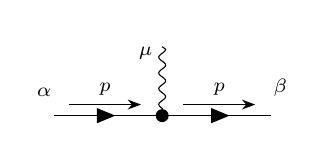
\begin{tikzpicture}[scale=1, transform shape]
    \begin{feynman}
    
    \vertex [label=\ensuremath{\scriptstyle \alpha}] (a) {};
    \vertex [dot, right=1.5cm of a] (b) {};
    \vertex [above=1cm of b] (c) {};
    \vertex [right=1.5cm of b, label=\ensuremath{\scriptstyle \beta}] (d) {};

    \diagram* {
      (a) -- [fermion, momentum={[arrow distance=4pt] \ensuremath{\scriptstyle p}}] (b), (b) -- [boson, edge label=\ensuremath{\scriptstyle \mu}, pos=0.9] (c), (b) -- [fermion, momentum={[arrow distance=4pt] \ensuremath{\scriptstyle p}}] (d)
    };
  \end{feynman}
\end{tikzpicture} &=& -ie\gamma^\mu_{\beta\alpha};
\end{eqnarray}
plus the rules for the external spinors and polarisations
\begin{enumerate}
    \item $u_{\alpha,s}(p,m)$ for the initial particle;
    \item $\ubar_{\alpha,s}(p,m)$ for the final particle;
    \item $\vbar_{\alpha,s}(p,m)$ for the initial antiparticle;
    \item $v_{\alpha,s}(p,m)$ for the final antiparticle;
    \item $\epsilon_\mu(p)$ for the initial photon;
    \item $\epsilon_\mu^*(p)$ for the final photon.
\end{enumerate}

\section{Superficial QED degree of divergence}
Recall, from equation \eqref{eq: superficial degree of divergence}, that $\omega(\Gamma_{\phi^3}) = DL - 2n_{\phi^3}$ where $D$ is the dimension, $L$ is the loop order, and $n_{\phi^3}$ the number of internal lines. We may derive a similar form for a graph in QED by 
\begin{equation}
    \omega(\Gamma_{QED}) = DL - 2n_\gamma - n_e,
\end{equation}
where $n_\gamma$ and $n_e$ are the number of internal photon and fermion lines respectively. We may in terms of external photon and electron multiplicity, $E_\gamma$ and $E_e$, using
\begin{equation}
    L = n_e + n_\gamma - V + 1,\quad V = 2n_\gamma + E_\gamma = n_e + \frac{E_e}{2},
\end{equation}
write that 
\begin{equation}
    \omega(\Gamma_{QED}) = D + \bigg(\frac{1 - D}{2}\bigg)E_e + \bigg(\frac{2 - D}{2}\bigg)E_\gamma + \bigg(\frac{D - 4}{2}\bigg)V,
\end{equation}
so in four dimensions $\omega(\Gamma_{QED})$ is simply
\begin{equation}
    \omega(\Gamma_{QED}) = 4 - \frac{3}{2}E_e - E_\gamma.
\end{equation}
In the following table \ref{tab: divergent QED graphs} are listed some divergent QED graphs. 
\begin{table}[h]
    \centering
    \begin{tabular}{|c|cccc|}
         \hline
         $\Gamma$ & $E_e$ & $E_\gamma$ & $\omega(\Gamma_{QED})$ & name  \\ \hline
         \feynmandiagram [inline=(v.base), scale=0.8, horizontal=a to v, transform shape] {
         a -- [photon] v [blob] 
         }; & 0 & 1 & 3 & tadpole \\
         \feynmandiagram [inline=(v.base), scale=0.8, horizontal=a to b, transform shape, layered layout] {
         a -- [fermion] v [blob] -- [fermion] b 
         }; & 2 & 0 & 1 & electron self energy \\
         \feynmandiagram [inline=(v.base), scale=0.8, horizontal=a to b, transform shape, layered layout] {
         a -- [photon] v [blob] -- [photon] b 
         }; & 0 & 2 & 2 & photon vacuum polarisation \\
         \feynmandiagram [inline=(a.base), layered layout, horizontal=a to b, scale=0.8, transform shape] {
        a -- [photon] b [blob] -- [fermion] c, b -- [anti fermion] d
        }; & 2 & 1 & 0 & vertex \\
        \feynmandiagram [inline=(a.base), layered layout, horizontal=a to b, scale=0.6, transform shape] {
        a -- [photon] b [blob] -- [photon] c, b -- [photon] d
        }; & 0 & 3 & 2 & - \\
        \feynmandiagram [inline=(v.base), scale=0.8, transform shape, rotate=-32] { a -- [photon] v [blob], b -- [photon] v, v -- [photon] c, v -- [photon] d, a -- [opacity=0.0] b, d -- [opacity=0.0] c, }; & 0 & 4 & 0 & - \\ \hline
    \end{tabular}
    \caption{some divergent graphs in QED.}
    \label{tab: divergent QED graphs}
\end{table}
The treatment of the tadpole graph is different, and more straightforward, than in $\phi^3$ where is was necessary to redefine the vacuum expectation value. Here we can show the graph is zero, for example at 1-loop
\begin{equation}
    \begin{split}
        \feynmandiagram [inline=(v.base), scale=0.8, horizontal=a to v, transform shape, layered layout] {
        a -- [photon, edge label = \(\mu\), pos=0.1] v, v -- [fermion, half left, looseness=1.5, momentum={[arrow distance=5pt, arrow shorten=0.2] \(\scriptstyle k\)}] v1, v1 -- [half left, looseness=1.5] v
        }; &= -ie\,\mathrm{tr}\bigg(\gamma^\mu\int_k\frac{\slk + m}{k^2 - m^2}\bigg) \\
        &= -ie\,\tr{\gamma^\mu}m\int_k\frac{1}{k^2 - m^2} - ie\,\tr{\gamma^\mu\gamma^\nu}\int_k\frac{k_\nu}{k^2 - m^2} \\
        &= 0.
    \end{split}
\end{equation}
This property holds to all loop orders so
\begin{equation}
    \feynmandiagram [inline=(v.base), scale=0.8, horizontal=a to v, transform shape] {
    a -- [photon] v [blob]
    }; = 0.
\end{equation}
There are two other graphs to worry about, which are the ones with $E_\gamma = 3$ and $E_\gamma = 4$. There are operators for $\gamma$ self interactions in the Lagrangian so it is not clear where to absorb the divergences. The resolution is to see that divergences cancel between contributing diagrams, for example
\begin{equation}
    \feynmandiagram [inline=(v.base), layered layout, horizontal=a to b, scale=0.8, transform shape] {
        a -- [photon, edge label = \(1\), pos=0.1] b [blob] -- [photon, edge label = \(2\), pos=0.5] c, b -- [photon, edge label'=\(3\), pos=0.5] d
        }; = \feynmandiagram [inline=(c.base), scale = 0.6] {
          a -- [bend left=60] b
            -- [bend left=60] c
            -- [fermion, bend left=60] a, i1 -- [photon, edge label = {\small \(3\)}] a, i2 -- [photon, edge label = {\small \(1\)}] b, i3 -- [photon, edge label =  {\small \(2\)}] c,
        }; + \feynmandiagram [inline=(c.base), scale = 0.6] {
          a -- [bend left=60] b
            -- [bend left=60] c
            -- [fermion, bend left=60] a, i1 -- [photon, edge label = {\small \(3\)}] a, i2 -- [photon, edge label = {\small \(2\)}] b, i3 -- [photon, edge label =  {\small \(1\)}] c,
        }; + o(e^5) = 0,
\end{equation}
and for the $E_\gamma = 4$ case 
\begin{equation} 
    \feynmandiagram [inline=(v.base), scale=0.8, horizontal=a to d, transform shape] { 
        a -- [photon, edge label={\small 1}, pos=0.1] v [blob], 
        b -- [photon, edge label={\small 2}, pos=0.1] v, 
        v -- [photon, edge label={\small 3}, pos=0.9] c, 
        v -- [photon, edge label={\small 4}, pos=0.9] d 
    }; = \feynmandiagram[ 
        inline={([yshift=-0.1cm]current bounding box.center)}, 
        scale=0.8, 
        transform shape, 
        horizontal=v1 to v2
    ] { 
        a -- [photon, edge label={\small 1}, pos=0.1] v1, 
        v1 -- v2, 
        v2 -- [photon, edge label={\small 2}, pos=0.9] b, 
        v2 -- v3, 
        v3 -- [photon, edge label={\small 3}, pos=0.9] c, 
        v3 -- v4, 
        v4 -- [fermion] v1, 
        v4 -- [photon, edge label={\small 4}, pos=0.9] d 
    }; + \mathrm{permutations} + o(e^6) = \mathrm{finite}. 
\end{equation}
Moreover, the $E_\gamma = 3$ graph, and technically also the tadpole graph, is a special case of a more general theorem, which follows using charge conjugation symmetry.
\begin{teo}[Furry's theorem]
    Correlations functions and amplitudes for odd numbers of photons are zero.
\end{teo}
In terms of bare quantities, the QED Lagrangian is
\begin{equation}
    \dL_{0,QED} = \frac{1}{2}A_0^\mu\bigg[\square g_{\mu\nu} - \bigg(1 - \frac{1}{\xi}\bigg)\p_\mu \p_\nu\bigg]A_0^\nu + i\psib_0\slpd\psi_0 - m_0\psib_0\psi_0 - e_0\psib_0\slA_0\psi_0.
\end{equation}
We relate bare quantities to renormalized ones using
\begin{gather}
    \psi_0 = \sqrt{Z_\psi}\psi_R,\quad A_0^\mu = \sqrt{Z_A} A_R^\mu,\quad m_0^2 = Z_mm_R^2, \\
    e_0 = Z_ee_R\mu_R^\epsilon = \frac{Z_1}{Z_\psi\sqrt{Z_A}}e_R\mu_R^\epsilon,\quad \xi_0 = \frac{Z_A}{Z_\xi}\xi_R,
\end{gather}
so that the Lagrangian becomes $\dL_{QED} = \dL_{QED,R} + \dL_{counter}$, where
\begin{equation}
    \begin{split}
        \dL_{counter} &= \frac{1}{2}(Z_A - 1)A_R^\mu(\square g_{\mu\nu} - \p_\mu\p_\nu)A_R^\nu + \frac{1}{2}\frac{Z_\xi - 1}{\xi_R}A_R^\mu\p_\mu\p_\nu A^\nu_R \\
        &+ i(Z_\psi - 1)\psib_R\slpd\psi_R - (Z_mZ_\psi - 1)m_R\psib_R\psi_R \\
        &- (Z_1 - 1)e_R\mu_R^\epsilon\psib_R\slA_R\psi_R,
    \end{split}
\end{equation}
which is invariant under gauge rotations
\begin{equation}
    \begin{cases}
        \psi_R \to \psi_R' = e^{i\theta(x)}\psi_R, \\
        A_R^\mu \to A_R'^\mu = A_R^\mu - \dfrac{1}{e_R\mu_R^\epsilon}\p^\mu\theta(x).
    \end{cases}
\end{equation}
For the whole expression to be invariant requires $Z_1 = Z_\psi$. The Feynman rules for the counter-terms are
\begin{align}
    \feynmandiagram[inline=(v.base), layered layout, horizontal=a to b, scale=0.8, transform shape] { 
    a -- [fermion, momentum'={[arrow distance=3.5pt]\(\scriptstyle p\)}, edge label=\(\alpha\), pos=0.1] v [crossed dot, pos=0.5] -- [fermion, edge label=\(\beta\), pos=0.9] b, 
    }; &= i(\slp\delta_\psi - m\delta_3)_{\beta\alpha}, \\
    \feynmandiagram[inline=(v.base), layered layout, horizontal=a to b, scale=0.8, transform shape] { 
    a -- [photon, momentum'={[arrow distance=3.5pt]\(\scriptstyle p\)}, edge label=\(\mu\), pos=0.1] v [crossed dot, pos=0.5] -- [photon, edge label=\(\nu\), pos=0.9] b, 
    }; &= -i(p^2g^{\mu\nu} - p^\mu p^\nu)\delta_A, \\
    \feynmandiagram[inline=(v.base),
    scale=0.8, horizontal=a to v, layered layout,
    transform shape] {
    a -- [fermion, momentum'={[arrow distance=3.5pt]\(\scriptstyle p\)}, edge label=\(\alpha\), pos=0.1] v [crossed dot] -- [fermion, edge label=\(\beta\), pos=0.9] b, v -- [photon, edge label=\(\mu\)] c
    }; &= -ie_R\mu_R^\epsilon\gamma^\mu\delta_1,
\end{align}
where
\begin{gather}
    \delta_3 = Z_mZ_\psi - 1,\quad \delta_\psi = Z_\psi - 1, \\
    \delta_A = Z_A - 1,\quad \delta_1 = Z_1 - 1.
\end{gather}
Moreover, later we will show that $Z_\xi = 1$. 

\section{Divergent graphs at one loop}
The expansions of the divergent graphs at 1-loop are
\begin{align}
    \begin{split}
        \feynmandiagram[inline=(v.base), layered layout, horizontal=a to b, scale=0.8, transform shape] { 
        a -- [fermion, momentum'={[arrow distance = 5pt]\(\scriptstyle p\)}, edge label=\(\beta\), pos=0.1] v [blob, pos=0.5] -- [fermion, edge label=\(\alpha\), pos=0.9] b, 
        }; &= \Sigma_{\alpha\beta}(p,m) = \feynmandiagram[inline=(v.base), layered layout, horizontal=a to b, scale=0.8, transform shape] { 
        a -- [fermion] v -- [photon, half left, looseness=1.5] v1, v --[fermion] v1, v1 --[fermion] b, 
        }; + \feynmandiagram[inline=(v.base), layered layout, horizontal=a to b, scale=0.8, transform shape] { 
        a -- [fermion] v [crossed dot, pos=0.5] -- [fermion] b, 
        }; + o(e^4),
    \end{split} \\
    \begin{split}
        \feynmandiagram[inline=(v.base), layered layout, horizontal=a to b, scale=0.8, transform shape] { 
        a -- [photon, momentum'={[arrow distance = 5pt]\(\scriptstyle p\)}, edge label=\(\mu\), pos=0.1] v [blob, pos=0.5] -- [photon, edge label=\(\nu\), pos=0.9] b, 
        }; &= \Pi_{\mu\nu}(p,m) = \feynmandiagram[inline=(v.base), layered layout, horizontal=a to b, scale=0.5, transform shape] { 
        a -- [photon] v -- [half left, looseness=1.5] v1 -- [half left, looseness=1.5] v, v1 -- [photon] b, }; + \feynmandiagram[inline=(v.base), layered layout, horizontal=a to b, scale=0.8, transform shape] { 
        a -- [photon] v [crossed dot] v1 -- [photon] b, }; + o(e^4),
    \end{split} \\
    \begin{split}
        \feynmandiagram [inline=(v.base), layered layout, horizontal=a to b, scale=0.8, transform shape] {
        a -- [fermion, edge label = \(\alpha\), pos=0.1] b [blob] -- [fermion, edge label = \(\beta\), pos=0.5] c, b -- [photon, edge label'=\(\mu\), pos=0.5, momentum={[arrow distance=4pt]\ensuremath{\scriptstyle p}}] d
        }; &= \Gamma^\mu_{\alpha\beta}(p,m) = \feynmandiagram[inline=(c.base), rotate=-45, horizontal=a to b, scale=0.75] {
        a -- v1 -- [anti fermion] v -- [anti fermion] v2 -- b, v1 -- [boson] v2, v -- [boson] c,
        }; + \feynmandiagram [inline=(d.base), layered layout, horizontal= c to d, scale=0.8, transform shape] {
        a -- [anti fermion] c [crossed dot], b -- [fermion] c, c -- [photon] d
        }; + o(e^5),
    \end{split}
\end{align}
which are the electron self-energy, the photon vacuum polarisation and the vertex correction, respectively.

\subsection{Electron self-energy}
Let's compute the electron self-energy in the Feynman gauge, defined as the imposition $\xi_R = 1$, as a simplification. So
\begin{equation}
    \begin{split}
        \feynmandiagram[inline=(v.base), layered layout, horizontal=a to b, scale=0.8, transform shape] { 
        a -- [fermion, momentum'={[arrow distance = 5pt]\(\scriptstyle p\)}, edge label=\(\beta\), pos=0.1] v -- [photon, momentum={[arrow distance = 5pt] \(\scriptstyle k\)}, half left, looseness=1.5] v1, v --[fermion, momentum'={[arrow distance = 5pt]\(\scriptstyle p-k\)}] v1, v1 --[fermion, edge label=\(\alpha\), pos=0.9] b, 
        }; &= (-ie_R\mu_R^\epsilon)^2\int_k\gamma_{\alpha\delta}^\mu\frac{(\slp - \slk + m_R)_{\delta\sigma}}{D(k - p, m_R)}\gamma^\nu_{\sigma\beta}\bigg(-\frac{ig_{\mu\nu}}{D(k,0)}\bigg) \\
        &= e_R^2\mu_R^{2\epsilon}\int_k\frac{[\gamma^\mu(\slk - \slp - m_R)\gamma_\mu]_{\alpha\beta}}{D(k,0)D(k - p, m_R)} \\
        &= e_R^2\mu_R^{2\epsilon}\int_k\frac{[(2 - D)(\slk - \slp) - Dm_R]_{\alpha\beta}}{D(k,0)D(k - p, m_R)},
    \end{split}
\end{equation}
now we define
\begin{equation}
    I^{(1)[D]}_{2,m_1,m_2}[N] = \int_k\frac{N}{D(k,m_1)D(k - p, m_2)},
\end{equation}
such that
\begin{equation}
    \feynmandiagram[inline=(v.base), layered layout, horizontal=a to b, scale=0.8, transform shape] { 
    a -- [momentum'={[arrow distance = 4pt]\(\scriptstyle p\)}] v -- [photon, half left, looseness=1.5] v1, v -- v1, v1 -- b, 
    }; = -e_R^2\mu_R^{2\epsilon}\{[(2 - D)\slp + Dm_R]I_{2,0,m}^{(1)[D]} - (2 - D)I_{2,0,m}^{(1)[D]}[\slk]\}
\end{equation}
and since,
\begin{equation}
    I_{2,0,m}^{(1)[D]}[\slk] = \slp b_1(p;0,m) = \frac{\slp}{2p^2}\{I_{1,m}^{(1)[D]}[1] + (p^2 - m_R^2)I_{2,0,m}^{(1)[D]}[1]\},
\end{equation}
we have
\begin{equation}
    \begin{split}
        \feynmandiagram[inline=(v.base), layered layout, horizontal=a to b, scale=0.8, transform shape] { 
        a -- [momentum'={[arrow distance = 4pt]\(\scriptstyle p\)}] v -- [photon, half left, looseness=1.5] v1, v -- v1, v1 -- b, 
        }; &= -e_R^2\mu_R^{2\epsilon}\bigg\{\frac{(2 - D)\slp}{2p^2}\bigg[(p^2 + 2m_R^2)I_{2,0,m}^{(1)[D]}[1] - I_{1,m}^{(1)[D]}[1]\bigg] \\
        &+ Dm_RI_{1,m}^{(1)[D]}[1]\bigg\}.
    \end{split}
\end{equation}
The scalar integrals in $D = 4 - 2\epsilon$ dimension are
\begin{align}
    \begin{split}
        I_{1,m}^{(1)[4 - 2\epsilon]}[1] &= \frac{i}{(4\pi)^{2 - \epsilon}}\frac{\Gamma(1 + \epsilon)}{(1 - \epsilon)\epsilon}(m_R^2)^{1 - \epsilon} \\
        &= \frac{ir_\Gamma}{(4\pi)^2}m_R^2\bigg[\frac{1}{\epsilon} + 1 -\log{(m_R^2)} + o(\epsilon)\bigg],
    \end{split} \\
    \begin{split}
        I_{2,0,m}^{(1)[4 - 2\epsilon]}[1] &= \frac{ir_\Gamma}{(4\pi)^2}\bigg[\frac{1}{\epsilon} + 2 - \log{(m_R^2)} + \bigg(1 - \frac{m_R^2}{p^2}\bigg)\log{\bigg(1 - \frac{m_R^2}{p^2}\bigg)} + o(\epsilon)\bigg],
    \end{split}
\end{align}
where we recall that $r_\Gamma \equiv \Gamma(1 + \epsilon)(4\pi)^\epsilon$ and so we find, using that $e_R^2 = 4\pi\alpha$, that
\begin{equation}
    \feynmandiagram[inline=(v.base), layered layout, horizontal=a to b, scale=0.8, transform shape] { 
    a -- [momentum'={[arrow distance = 4pt]\(\scriptstyle p\)}] v -- [photon, half left, looseness=1.5] v1, v -- v1, v1 -- b, 
    }; = \frac{i\alpha}{4\pi}(\slp - 4m_R)\frac{1}{\epsilon} + o(\epsilon^0).
\end{equation}

\subsection{Photon vacuum polarisation}
Let's now compute the photon vacuum polarisation, again by setting ourselves in the Feynman gauge. So we have
\begin{equation}
    \feynmandiagram[inline=(v.base), layered layout, horizontal=a to b, scale=0.8, transform shape] 
    { a -- [photon, edge label=\(\mu\)] v -- [half left, looseness=1.5, momentum={[arrow distance=3pt, arrow shorten=0.2] \(\scriptstyle k\)}] v1 -- [half left, looseness=1.5, momentum = {[arrow distance=3pt, arrow shorten=0.2] \(\scriptstyle k-p\)}] v, v1 -- [photon, edge label=\(\nu\)] b, 
    }; = -(-ie_R\mu_R^\epsilon)^2\int_k\frac{\mathrm{tr}[{\gamma^\mu i(\slk + m_R)\gamma^\nu i(\slk - \slp +m_R)]}}{D(k, m_R)D(k - p, m_R)},
\end{equation}
where the numerator can be written as
\begin{multline}
    \mathrm{tr}[{\gamma^\mu i(\slk + m_R)\gamma^\nu i(\slk - \slp +m_R)]} = \\ 
    = 4(2k^\mu k^\nu - k^2g^{\mu\nu} - k^\mu p^\nu - k^\nu p^\mu + k_\lambda p^\lambda g^{\mu\nu} + m_R g^{\mu\nu})
\end{multline}
so we need the tensor reduction for up to rank two bubble integrals. After applying Passarino-Veltmann reduction one finds
\begin{equation}
    \feynmandiagram[inline=(v.base), layered layout, horizontal=a to b, scale=0.8, transform shape] { 
    a -- [photon, edge label=\(\mu\)] v -- [half left, looseness=1.5] v1 -- [half left, looseness=1.5] v, v1 -- [photon, edge label=\(\nu\)] b, 
    }; = -e_R^2\mu_R^{2\epsilon}(-g^{\mu\nu}p^2 + p^\mu p^\nu)A,
\end{equation}
where we set
\begin{equation}
    A \equiv \frac{4}{p^2(D - 1)}\bigg[(D - 2)I_{1,m}^{(1)[D]} - \bigg(2m_R^2 + \frac{D - 2}{2}p^2\bigg)I_{2,m,m}^{(1)[D]}\bigg].
\end{equation}
The bubble integral is the same we used in the $\phi^3$ theory, so in $D = 4 - 2\epsilon$ dimensions one can show that
\begin{equation} 
    \feynmandiagram[inline=(v.base), layered layout, horizontal=a to b, scale=0.8, transform shape] { 
    a -- [photon, edge label=\(\mu\)] v -- [half left, looseness=1.5] v1 -- [half left, looseness=1.5] v, v1 -- [photon, edge label=\(\nu\)] b, }; = -\frac{i\alpha}{4\pi}(-g^{\mu\nu}p^2 + p^\mu p^\nu)\bigg[-\frac{4}{3\epsilon} + o(\epsilon^0)\bigg]. 
\end{equation}

\subsection{Vertex correction}
This computation requires considerable extra work and is necessary to fix $\delta_1^{(1)}$. If we accept the result $Z_1 = Z_2$ then we can avoid the computation but validating the result is an extremely good cross check. The one loop diagram is
\begin{equation}
    \feynmandiagram[
    inline=(v1.base), horizontal=a to b, scale=0.9, transform shape] {
    a -- [fermion, momentum'=\(\scriptstyle p_1\)] v1 -- [fermion, momentum=\(\scriptstyle k+p_1\)] v -- [fermion, momentum=\(\scriptstyle k+p_2\)] v2 -- [fermion, momentum'=\(\scriptstyle p_2\)] b, v1 -- [boson, momentum'=\(\scriptstyle k\)] v2, v -- [boson, momentum'=\(\scriptstyle p_3\)] c,
    }; = -ie_R\mu_R^\epsilon\ubar(p_2,m_R)\Gamma^{(1)\mu}u(p_1,m_R),
\end{equation}
where, in the Feynman gauge, $\Gamma^{(1)\mu}$ is
\begin{equation}
    \Gamma^{(1)\mu} = -i^3(-ie_R\mu_R^\epsilon)^2\int_k\frac{\gamma^\nu(\slk + \slp_2 + m_R)\gamma^\mu(\slk + \slp_1 + m_R)\gamma_\nu}{D(k,0)D(k + p_1,m_R)D(k + p_2, m_R)}.
\end{equation}
A general basis for $\Gamma^\mu_{\alpha\beta}(p_1,p_2)$ would have three elements $\gamma^\mu_{\alpha\beta}$, $p_1^\mu\delta_{\alpha\beta}$ and $p_2^\mu\delta_{\alpha\beta}$. However, $\Gamma^{(1)\mu}$ satisfies the Ward identity
\begin{equation}
    \Gamma^{(1)\mu}(p_1,p_2)p_{3\mu} = \Gamma^{(1)\mu}(p_1,p_2)(p_1 - p_2)_\mu = 0.
\end{equation}
As a result, $\Gamma^{(1)\mu}$ can be described in terms of two independent tensor structures. The vertex describes the electromagnetic interaction and so it is useful to use a tensor basis that exposes electric and magnetic properties. Thus, we define
\begin{equation}
    \Gamma^{(1)\mu}(p_1,p_2) = F_1\gamma^\mu + F_2\frac{i\sigma^{\mu\nu}}{2m_R}(-p_1 + p_2)_\nu,
\end{equation}
where $\sigma^{\mu\nu} = -i\comm{\gamma^\mu}{\gamma^\nu}/2$ and $F_1$ and $F_2$ are the electric and magnetic structure functions respectively. To prove the $\Gamma^{(1)\mu}$ decomposition we start from 
\begin{equation}
    \ubar_2\Gamma^{(1)\mu}u_1 = a_0\ubar_2\gamma^\mu u_1 + a_1p_1^\mu\ubar_2u_1 + a_2p_2^\mu\ubar_2u_1 
\end{equation}
and perform a base change to $(p_1 + p_2)_\mu$ and $(p_1 - p_2)_\mu$, thus getting
\begin{equation}
    \ubar_2\Gamma^{(1)\mu}u_1 = a_0\ubar_2\gamma^\mu u_1 + \tilde{a}_1(p_1 - p_2)^\mu\ubar_2u_1 + \tilde{a}_2(p_1 + p_2)^\mu\ubar_2u_1.
\end{equation}
Now, the Ward identity is satisfied if $\ubar_2\Gamma^{(1)\mu}p_{3\mu}u_1 = 0$, hence we get
\begin{equation}
    \begin{split}
        \ubar_2\Gamma^{(1)\mu}p_{3\mu}u_1 &= -\ubar_2\Gamma(p_1 - p_2)_\mu u_1 \\
        &= -a_0\ubar_2(\slp_1 - \slp_2)u_1 -\tilde{a}_1(p_1 - p_2)^2\ubar_2u_1 - \tilde{a}_2(p_1^2 - p_2^2)\ubar_2u_1 \\
        &= -\tilde{a}_1(p_1 - p_2)^2\ubar_2u_1 \\
        &= 0,
    \end{split}
\end{equation}
from this, since $-a_0\ubar_2(\slp_1 - \slp_2)u_1 = 0$ because $\ubar_2\slp_2 = m\ubar_2$ and $\slp_1u_1 = mu_1$ and since $\tilde{a}_2(p_1^2 - p_2^2)\ubar_2u_1$ because $p_1^2 = p_2^2 = m_R^2$, it follows that $\tilde{a}_1 = 0$. Now, we notice that
\begin{equation}
    p^\mu\ubar_2u_1 = p_\nu g^{\nu\mu}u_2u_1 = \frac{1}{2}p_\nu u_2\acomm{\gamma^\mu}{\gamma^\nu}u_1 = \frac{1}{2}u_2\acomm{\gamma^\mu}{\slp}u_1,
\end{equation}
hence
\begin{equation}
    \begin{split}
        (p_1 + p_2)^\mu\ubar_2u_1 &= \frac{1}{2}\ubar_2\acomm{\gamma^\mu}{\slp_1 + \slp_2}u_1 \\
        &= \frac{1}{2}\ubar_2(\gamma^\mu\slp_2 + \slp_1\gamma^\mu + 2m_R\gamma^\mu)u_1,
    \end{split}
\end{equation}
now we expand the magnetic tensor
\begin{equation}
    \begin{split}
        \ubar_2\bigg[\frac{i\sigma^{\mu\nu}}{2m_R}(-p_1 + p_2)_\nu \bigg]u_1 &= \frac{1}{4m_R}\ubar_2\comm{\gamma^\mu}{-\slp_1 + \slp_2}u_1 \\
        &= \frac{1}{4m_R}\ubar_2(\gamma^\mu\slp_2 + \slp_1\gamma^\mu - 2m_R\gamma^\mu)u_1 \\
        &= \frac{1}{2m_R}(p_1 + p_2)^\mu\ubar_2u_1 - \ubar_2\gamma^\mu u_1,
    \end{split}
\end{equation}
which completes the rearrangement. The full computation of the vertex diagram is quite long, but it is useful to try it in different ways.

\subsection{1-loop counter terms}
In the $\MMS$ scheme we can determine the values for $\delta_1$, $\delta_\psi$, $\delta_3$ and $\delta_A$. Thus from 
\begin{equation}
        \feynmandiagram[inline={([yshift=-0.1cm]current bounding box.center)}, rotate=-45, horizontal=a to b, scale=0.7] {
        a -- [momentum={[arrow distance=4pt]\ensuremath{\scriptstyle p_1}}] v1 -- [fermion] v -- [anti fermion] v2 -- [momentum={[arrow distance=4pt]\ensuremath{\scriptstyle p_2}}] b, v1 -- [boson] v2, v -- [boson, momentum={[arrow distance=4pt]\ensuremath{\scriptstyle p_3}}] c,
        }; + \feynmandiagram [inline={([yshift=-0.1cm]current bounding box.center)}, layered layout, horizontal= c to d, scale=0.8, transform shape] {
        a -- c [crossed dot], b -- c, c -- [photon] d
        }; = \mathrm{finite}
\end{equation}
we get
\begin{equation}
    \delta_1^{(1)} = \frac{\alpha}{4\pi}r_\Gamma\bigg(-\frac{1}{\epsilon}\bigg),
\end{equation}
from
\begin{equation}
    \feynmandiagram[inline={([yshift=-0.1cm]current bounding box.center)}, layered layout, horizontal=a to b, scale=0.7, transform shape] { 
    a -- [momentum'={[arrow distance = 4pt]\ensuremath{\scriptstyle p}}] v -- [photon, half left, looseness=1.5] v1, v -- v1, v1 -- b, 
    }; + \feynmandiagram [inline={([yshift=-0.1cm]current bounding box.center)}, layered layout, horizontal= a to c, scale=0.8, transform shape] {
    a -- b [crossed dot], b -- c
    }; = \mathrm{finite}
\end{equation}
we get
\begin{equation}
    \delta_\psi^{(1)} = \dfrac{\alpha}{4\pi}r_\Gamma\bigg(-\dfrac{1}{\epsilon}\bigg),\quad \delta_3^{(1)} = \dfrac{\alpha}{4\pi}r_\Gamma\bigg(-\dfrac{4}{\epsilon}\bigg),
\end{equation}
and from
\begin{equation}
    \feynmandiagram[inline={([yshift=-0.1cm]current bounding box.center)}, layered layout, horizontal=a to b, scale=0.5, transform shape] { a -- [photon] v -- [half left, looseness=1.5] v1 -- [half left, looseness=1.5] v, v1 -- [photon] b}; + \feynmandiagram [inline={([yshift=-0.1cm]current bounding box.center)}, layered layout, horizontal= a to c, scale=0.8, transform shape] {
    a -- [photon] b [crossed dot], b -- [photon] c
    }; = \mathrm{finite}
\end{equation}
we get
\begin{equation}
    \delta_A^{(1)} = \frac{\alpha}{4\pi}r_\Gamma\bigg(-\frac{4}{3\epsilon}\bigg).
\end{equation}
From the constants we may obtain 
\begin{equation}
    \delta_e^{(1)} = -\frac{1}{2}\delta_A^{(1)} = \frac{\alpha}{4\pi}r_\Gamma\bigg(-\frac{3}{2\epsilon}\bigg),\quad \delta_m^{(1)} = \delta_3^{(1)} - \delta_\psi^{(1)} = \frac{\alpha}{4\pi}r_\Gamma\bigg(-\frac{3}{\epsilon}\bigg).
\end{equation}
The Dyson re-summed electron propagator is 
\begin{equation}
    \frac{1}{\slp - m_R + \Sigma_R(\slp,m_R)}
\end{equation}
and we would like to ensure the propagator has no quantum corrections, namely $\Sigma_R = 0$, at the physical pole $m_R = m_P$. We may expand the self-energy $\Sigma_R$ around $\slp = m_R\MI$ to obtain
\begin{multline}
    \Sigma_R(\slp,m_R) = \Sigma_R(\slp,m_R)|_{\slp=m_R} + (\slp-m_R)\Sigma_R^{WF}(p^2,m_R^2) + o[(\slp - m_R)^2],
\end{multline}
where
\begin{equation}
    \Sigma_R^{WF}(p^2,m_R^2) \equiv \frac{d}{d\slp}\Sigma_R(\slp,m_R)|_{\slp = m_R}.
\end{equation}
So to completely fix $\delta_\psi$ and $\delta_m$ in the on-shell scheme we must impose
\begin{align}
    \Sigma_R(\slp,m_R)|_{\slp=m_R} &= 0, \\
    \frac{d}{d\slp}\Sigma_R(\slp,m_R)|_{\slp=m_R} &= 0.
\end{align}
The photon counter-term can be fixed at zero momentum
\begin{equation}
    \lim_{p^2\to 0}\Pi(p^2,m_R^2) = 0,
\end{equation}
and the vertex correction can be fixed to a measurement at low $Q^2$
\begin{equation}
    \lim_{Q^2\to 0}\Gamma^\mu_R(Q^2,m_R^2) = -ie_P\gamma^\mu,
\end{equation}
where $Q^2 \to 0$ means that we are far away from the interaction point. There's a subtlety regarding the on-shell scheme renormalization constants in that the finite part of the vertex correction had on the IR divergence: the wave-function renormalization condition $d\Sigma/d\slp|_{\slp=m_R} = 0$ also contains an IR divergence such that we obtain $Z_\psi = Z_1$ as expected.

\section{Re-summation of photon propagator}
For $\xi_R = 1$ the Fourier transformed $2$-photon Green function is
\begin{equation}
    \begin{split}
        \tilde{G}_{\mu\nu}(p^2) &= \feynmandiagram[inline={([yshift=-0.1cm]current bounding box.center)}, layered layout, horizontal=a to b, scale=0.6, transform shape] { a -- [photon] b }; + \feynmandiagram[inline={([yshift=-0.1cm]current bounding box.center)}, layered layout, horizontal=a to b, scale=0.6, transform shape] { a -- [photon] v [blob] -- [photon] b }; + \feynmandiagram[inline={([yshift=-0.1cm]current bounding box.center)}, layered layout, horizontal=a to b, scale=0.6, transform shape] { a -- [photon] v [blob] -- [photon] v1 [blob] -- [photon] b }; + \cdots \\
        &= -\frac{ig_{\mu\nu}}{p^2} + \frac{ig_{\mu\sigma}}{p^2}\Pi^{\sigma\rho}\frac{ig_{\rho\nu}}{p^2} - \frac{ig_{\mu\sigma}}{p^2}\Pi^{\sigma\rho}\frac{ig_{\rho\lambda}}{p^2}\Pi^{\lambda\delta}\frac{ig_{\delta\nu}}{p^2} + \cdots,
    \end{split}
\end{equation}
where $\Pi^{\mu\nu} \equiv i(p^2g^{\mu\nu} - p^\mu p^\nu)\Pi$, such that
\begin{equation}
    \begin{split}
        \tilde{G}_{\mu\nu} &= -\frac{ig_{\mu\nu}}{p^2} + \frac{i}{p^4}(p^2g_{\mu\nu} - p_\mu p_\nu)\Pi - \frac{i}{p^6}(p^2g_{\mu\nu} - p_\mu p_\nu)(p^2 g^\nu_\nu - p^\nu p_\nu)\Pi^2 \\
        &= -\frac{i}{p^4}(p^2g_{\mu\nu} + p_\mu p_\nu)(1 - \Pi + \Pi^2 + \cdots) - \frac{ip_\mu p _\nu}{p^4} \\
        &= -\frac{i}{p^2}\bigg(g_{\mu\nu} - \frac{p_\mu p_\nu}{p^2}\bigg)\frac{1}{1 + \Pi} - \tilde{G}_{\mu\nu,L},
    \end{split}
\end{equation}
where we denoted $\tilde{G}_{\mu\nu,L} \equiv -ip_\mu p_\nu/p^4$. In this way, we see that only the transverse part of the photon propagator is affected. The longitudinal component, $\tilde{G}_{\mu\nu,L}$, does not contribute to physical quantities thanks to the Ward identity. We can also prove that $Z_\xi = 1$. In particular, we can show that gauge invariance dictates $Z_\xi = 1$ by studying the 2-photon Green function, from $\tilde{G}_{\mu\nu,0}(p^2,\xi_0) = Z_A\tilde{G}_{\mu\nu,R}(p^2,\xi_R)$, we get
\begin{multline}
    -\frac{i}{p^2}\bigg(g_{\mu\nu} - \frac{p_\mu p_\nu}{p^2}\bigg)\frac{1}{1 + \Pi_0} - \frac{i\xi_0 p_\mu p_\nu}{p^2} = \\
    = \bigg[-\frac{i}{p^2}\bigg(g_{\mu\nu} - \frac{p_\mu p_\nu}{p^2}\bigg)\frac{1}{1 + \Pi_R} - \frac{i\xi_R p_\mu p_\nu}{p^2}\bigg]Z_A,
\end{multline}
so from the coefficient of $g_{\mu\nu}$ we have
\begin{equation}
    \frac{1}{1 + \Pi_0} = \frac{Z_A}{1 + \Pi_R},
\end{equation}
while from the coefficient of $p_\mu p_\nu/p^2$ minus the one of $g_{\mu\nu}$ we have
\begin{equation}
    \xi_0 = Z_A\xi_R,
\end{equation}
but by definition $\xi_0 = Z_A\xi_R/Z_\xi$, so we are only consistent if $Z_\xi = 1$. 

\subsubsection{Interpretation of \texorpdfstring{$F_1$}{F1} and \texorpdfstring{$F_2$}{F2} corrections}
We now want to show that there is a direct connection between electric and magnetic interactions and the structure functions $F_1$ and $F_2$ by considering the interaction between an electron and a slowly varying semi-classical photon field $A^\mu_{c}$,
\begin{equation}
    \feynmandiagram[inline={([yshift=-0.1cm]current bounding box.center)}, scale = 0.85, horizontal=a to c] { 
    a -- [fermion] b [blob] -- [photon, reversed momentum={[arrow distance=4pt] \ensuremath{\scriptstyle q}}, edge label'=\ensuremath{\scriptstyle A_c^\mu}] d [dot], b -- [fermion] c}; = -ie_R\mu_R^\epsilon\psib\gamma_\mu\psi A^\mu_c + \cdots. 
\end{equation}
By taking the limit for $q^2 \to 0$ and the slow variation, namely $q^\mu \simeq \p/\p x^\mu$, we can expand the interaction as follows
\begin{equation}
\begin{aligned}
    \feynmandiagram[inline={([yshift=-0.1cm]current bounding box.center)}, scale = 0.85, horizontal=a to c] { 
    a -- [fermion, edge label=\ensuremath{\scriptstyle 1}] b [blob] -- [photon, edge label=\ensuremath{\scriptstyle A_c^\mu}] d [dot], b -- [fermion, edge label=\ensuremath{\scriptstyle 2}] c};
    &= \feynmandiagram[inline={([yshift=-0.1cm]current bounding box.center)}, scale = 0.85, horizontal=a to c] { 
    a -- [fermion] b -- [photon] d [dot], b -- [fermion] c}; + 
    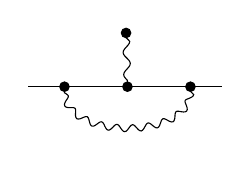
\begin{tikzpicture}[scale=0.8, transform shape, baseline={([yshift=-0.1cm]current bounding box.center)}]
    \begin{feynman}
    
    \vertex (a);
    \vertex [dot, right=0.5cm of a] (v1) {};
    \vertex [dot, right=2cm of v1] (v2) {};
    \vertex [dot, right=1cm of v1] (centro) {};
    \vertex [dot, right=0.5cm of v2] (b);
    \vertex [dot, above right=0.8cm and 1.5cm of a] (up) {};

    \diagram* {
      (a) -- (v1) -- (v2) -- (b),
      (v1) -- [photon, bend right=90] (v2), (centro) -- [photon] (up),
    };
    \end{feynman}
    \end{tikzpicture} +  \feynmandiagram[inline={([yshift=-0.1cm]current bounding box.center)}, scale = 0.7, horizontal=a to c] { 
    a -- [fermion] b [crossed dot] -- [photon] d [dot], b -- [fermion] c}; + \feynmandiagram[inline={([yshift=-0.1cm]current bounding box.center)}, horizontal=a to c, scale=0.7, transform shape, rotate=45] { a -- b -- c, b -- [photon] b1 -- [half left, looseness=1.5] v -- [half left, looseness=1.5] b1, v -- [photon] d [dot] }; \\
    &+ \feynmandiagram[inline={([yshift=-0.1cm]current bounding box.center)}, horizontal=a to c, scale=0.7, transform shape, rotate=45] { a -- b -- c, b -- [photon] b1 [crossed dot] -- [photon] d [dot]}; + \cdots \\
    &= -ie_R\mu_R^\epsilon\ubar_2[\gamma_\mu + \Gamma^{(1)}_{\mu,R}(q^2,m_R^2) + \gamma_\nu D^{\nu\rho}\Pi^{(1)}_{\rho\mu,R}(q^2,m_R^2)] \\
    &\times u_1A^\mu_c + o(e^5) \\
    &= \tilde{J}_\mu A^\mu_c.
    \end{aligned}
\end{equation}
The interaction is described by an effective Hamiltonian 
\begin{equation}
    \Delta H_{int} = \int d^3x\,J_\mu A^\mu_c,
\end{equation}
where $J_\mu$ is the Fourier transform of $\tilde{J}_\mu$. Let's look at $\ubar_2\Gamma^{(1)}_{\mu,R}u_1$ first
\begin{equation}
    \ubar_2\Gamma^{(1)}_{\mu,R}u_1 = u_2\gamma_\mu u_1 F^{(1)}_{1,R}(q^2,m_R^2) + \frac{i}{2m}\ubar_2\sigma_{\mu\nu}u_1(p_1 + p_2)^\nu F_{2,R}^{(1)}(q^2,m_R^2),
\end{equation}
where we can show that 
\begin{align}
    \lim_{q^2\to 0}F_{1,R}^{(1)}(q^2,m_R^2) &= \frac{\alpha}{4\pi}\frac{q^2}{m_R^2}[a + b(\mathrm{IR\,divergence})], \\
    \lim_{q^2\to 0}F_{2,R}^{(1)}(q^2,m_R^2) &= \frac{\alpha}{2\pi}.
\end{align}
\begin{obs}
    Renormalization has explicitly removed leading terms $(q^2/m_R^2)^0$ in the exposition of $F_1$.
\end{obs}
We may also look at the second term proportional to $\Pi^{(1)}$ in the same limit to find that
\begin{equation}
    \lim_{q^2\to 0}[\gamma_\nu D^{\nu\rho}\Pi^{(1)}_{\rho\mu,R}(q^2,m_R^2)] = \frac{C\alpha}{4\pi}\gamma_\mu\frac{q^2}{m_R^2},\quad C \in \R.
\end{equation}
In position space we have $q^2/m_R^2 \to \square/m_R^2$, so having examined the elements of $\tilde{J}_\mu$, we may return to the expression of $\Delta H_{int}$ and show 
\begin{equation}
    \begin{split}
        \Delta H_{int} &\propto e_R\int d^3x\,\bigg\{\psib\overset{\leftrightarrow}{\p}_\mu\psi\bigg[1 + \frac{\alpha}{4\pi}(a + c + b(\mathrm{IR\,divergence}))\square\bigg]A^\mu_c \\
        &+ \frac{1}{2m_R}\bigg(\frac{1}{2} + \frac{\alpha}{4\pi}\bigg)\psib\sigma^{\mu\nu}\psi F_{\mu\nu,c}\bigg\},
    \end{split}
\end{equation}
where $F_{\mu\nu,c} = \p_\mu A_{\nu,c} - \p_\nu A_{\mu,c}$, also the first part is the electric current, while the second is the magnetic moment of the electron. From the semi-classical Dirac equation one finds that 
\begin{equation}
    \vmu_{Dirac} = \frac{e}{2m_R}(2\vs) = g_{Dirac}\bigg(\frac{e}{4m_R}\vsigma\bigg),\quad g_{Dirac} = 2.
\end{equation}
The first order correction to the coupling constant $g_{Dirac}$ is therefore
\begin{equation}
    g_{Dirac} - 2 = \frac{\alpha}{\pi},
\end{equation}
which is the result obtained by Schwinger. 

\subsubsection{Interpretation of \texorpdfstring{$\Pi(p^2,m^2)$}{Pi}}
The renormalized 2-point function $\Pi_R(p^2,m_R^2)$ has implications for the range of the electromagnetic interaction. If we consider a static photon, namely with $q^0 = 0$ and so $q^2 = -|\vq|^2$, then for $|\vq|^2 \ll 1$ we have
\begin{equation}
    \lim_{q^2\to 0}\Pi_R(-|\vq|^2,m_R^2) = \frac{4}{15}\frac{|\vq|^2}{m_R^2} + o\bigg(\frac{|\vq|^4}{m_R^4}\bigg).
\end{equation}
The Dyson re-summed propagator gave us 
\begin{equation}
    \feynmandiagram[inline={([yshift=-0.1cm]current bounding box.center)}, layered layout, horizontal=a to b, scale=0.8, transform shape] { 
    a -- [photon] b, 
    }; + \feynmandiagram[inline={([yshift=-0.1cm]current bounding box.center)}, layered layout, horizontal=a to b, scale=0.5, transform shape] { a -- [boson] v -- [half left, looseness=1.5] v1 -- [half left, looseness=1.5] v, v1 -- [boson] b}; + \cdots,
\end{equation}
where we have used a cross at the end points to show we are propagating between two points far apart, namely in the limit $q^2 \to 0$, so
\begin{equation}
    \feynmandiagram[inline={([yshift=-0.1cm]current bounding box.center)}, layered layout, horizontal=a to b, scale=0.8, transform shape] { a -- [photon] b }; = \frac{(-ie_R)^2}{-|\vq|^2} = \frac{e_R^2}{|\vq|^2},
\end{equation}
so the Dyson re-summed expression is 
\begin{equation}
    \frac{e_R^2}{|\vq|^2}\bigg[\frac{1}{1 + \Pi_R(-|\vq|^2,m_R^2)}\bigg] = \frac{e_R^2}{|\vq|^2}\bigg[1 + \frac{\alpha}{4\pi}\frac{4}{15}\frac{|\vq|^2}{m_R^2} + o(\alpha^2)\bigg].
\end{equation}
We can use this result to read off the potential between a heavy nucleus of charge $-Ze$ and an electron 
\begin{equation}
    V(r) = -\frac{Ze_R^2}{4\pi|\vr|}\bigg[1 + \frac{\alpha}{4\pi}\frac{4}{15}\frac{\Delta(\vr)}{m_R^2} + o(\alpha^2)\bigg].
\end{equation}
The correction to $V(r)$ is called the Uehling potential and results in a charge screening effect. Also, $\Delta(\vr) \simeq \delta^{(3)}(\vr)$ but can be computed exactly to be a distribution concentrated in a region $r \le 1/m \simeq \lambda$, where $\lambda$ is the Compton wavelength. So for $r \ge 1/m$ the virtual $e^+e^-$ pairs accounted in $\Pi_R$ effect the medium around the electron reducing the effective electric charge. This effect is known as vacuum polarisation. We can also consider the effective coupling at very small distances by taking $|\vq|^2 \ge m_R^2$ in which gives 
\begin{equation}
    \Pi_R(-|\vq|^2,m_R^2) \xrightarrow{|\vq|^2 \gg m_R^2} \frac{\alpha}{4\pi}\frac{4}{9}\bigg[-5 + 3\log{\bigg(\frac{|\vq|^2}{m_R^2}\bigg)}\bigg] + o\bigg(\frac{m^2}{|\vq|^2}\bigg),
\end{equation}
thus the effective fine structure constant is
\begin{equation}
    \alpha_{eff}(|\vq|^2) \overset{|\vq|^2 \gg m_R^2}{=} \frac{\alpha}{1 - \dfrac{\alpha}{3\pi}\log{\bigg(\dfrac{|\vq|^2}{Am_R^2}\bigg)}},\quad A = e^{5/3}.
\end{equation}
From this, it is immediate to see that $\alpha_{eff} > \alpha$ at small distances. 

\section{Ward-Takashi identity}
We have already encountered the Ward identity of the form $A^\mu p_\mu = 0$, for an amplitude $A = A^\mu\epsilon_\mu(p)$. However, there is a stronger statement that applies to off-shell correlation functions from which the Ward identity follows, that is the Ward-Takahashi identity. To derive it, let's first take a correlation function with $n$ $e^+e^-$ pairs and $m$ photons $\gamma$, so
\begin{equation}
    M^\mu(p_1,\dots,p_n;q_1,\dots,q_n;r_1,\dots,r_m),
\end{equation}
where $p_i$ are incoming fermions, $q_i$ are outgoing fermions, and $r_i$ are outgoing photons. An incoming photon with momentum $k^\mu$ is inserted at all points along the $e^+e^-$ currents. The Ward-Takahashi identity states
\begin{equation}
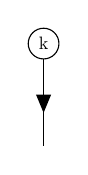
\begin{tikzpicture}[scale=0.65, transform shape, baseline={([yshift=0cm]current bounding box.center)}]
    \begin{feynman}
        
        \vertex [draw,circle,minimum size=0.6cm,inner sep=0pt] (k) {k};
        \vertex [below=2cm of k] (down);

        \diagram*{

            (k) -- [fermion] (down),
        };

    \end{feynman}
\end{tikzpicture}
\otimes
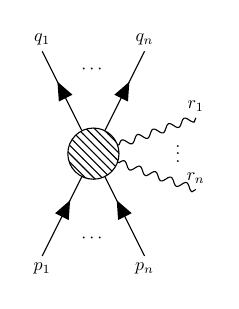
\begin{tikzpicture}[scale=0.65, transform shape, baseline={([yshift=-0.1cm]current bounding box.center)}]
    \begin{feynman}
        
        \vertex [blob, minimum size=1cm] (v) {};

        \vertex [above left=2cm and 1cm of v, label=\ensuremath{ q_1}] (q1);
        \vertex [above right=2cm and 1cm of v, label=\ensuremath{ q_n}] (qn);

        % p
        \vertex [below left=2cm and 1cm of v, label={[label distance=0.5pt]below:\ensuremath{ p_1}}] (p1);
        \vertex [below right=2cm and 1cm of v, label={[label distance=0.5pt]below:\ensuremath{ p_n}}] (pn);

        % r
        \vertex [above right=0.7 and 2cm of v, label=\ensuremath{ r_1}] (r1);
        \vertex [below right=0.7 and 2cm of v, label=\ensuremath{ r_n}] (rn);

        \diagram*{

            (v) -- [fermion] (q1),
            (v) -- [fermion] (qn),

            (v) -- [anti fermion] (p1),
            (v) -- [anti fermion] (pn),

            (v) -- [photon] (r1),
            (v) -- [photon] (rn)
        };

         \node at ($(q1)!0.5!(qn)+(0,-0.35)$) {$\cdots$};
         \node at ($(p1)!0.5!(pn)+(0,0.35)$) {$\cdots$};
         \node at ($(r1)!0.5!(rn)+(-0.35,0.1)$) {$\vdots$};

    \end{feynman}
\end{tikzpicture}
 = e_R\sum_{i=1}^n
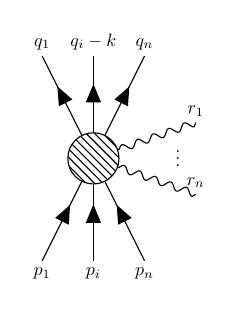
\begin{tikzpicture}[scale=0.65, transform shape, baseline={([yshift=-0.1cm]current bounding box.center)}]
    \begin{feynman}
        
        \vertex [blob, minimum size=1cm] (v) {};

        \vertex [above left=2cm and 1cm of v, label=\ensuremath{ q_1}] (q1);
        \vertex [above right=2cm and 1cm of v, label=\ensuremath{ q_n}] (qn);
        \vertex [above =2cm of v, label=\ensuremath{ q_i - k}] (qi-k);

        % p
        \vertex [below left=2cm and 1cm of v, label={[label distance=0.5pt]below:\ensuremath{ p_1}}] (p1);
        \vertex [below right=2cm and 1cm of v, label={[label distance=0.5pt]below:\ensuremath{ p_n}}] (pn);
        \vertex [below =2cm of v, label={[label distance=0.5pt]below:\ensuremath{ p_i}}] (pi);

        % r
        \vertex [above right=0.7 and 2cm of v, label=\ensuremath{ r_1}] (r1);
        \vertex [below right=0.7 and 2cm of v, label=\ensuremath{ r_n}] (rn);

        \diagram*{

            (v) -- [fermion] (q1),
            (v) -- [fermion] (qn),

            (v) -- [anti fermion] (p1),
            (v) -- [anti fermion] (pn),

            (v) -- [photon] (r1),
            (v) -- [photon] (rn),

            (v) -- [anti fermion] (pi),
            (v) -- [fermion] (qi-k),
        };

         \node at ($(r1)!0.5!(rn)+(-0.35,0.1)$) {$\vdots$};

    \end{feynman}
\end{tikzpicture}
-
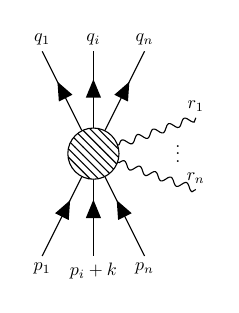
\begin{tikzpicture}[scale=0.65, transform shape, baseline={([yshift=-0.1cm]current bounding box.center)}]
    \begin{feynman}
        
        \vertex [blob, minimum size=1cm] (v) {};

        \vertex [above left=2cm and 1cm of v, label=\ensuremath{ q_1}] (q1);
        \vertex [above right=2cm and 1cm of v, label=\ensuremath{ q_n}] (qn);
        \vertex [above =2cm of v, label=\ensuremath{ q_i}] (qi);

        % p
        \vertex [below left=2cm and 1cm of v, label={[label distance=0.5pt]below:\ensuremath{ p_1}}] (p1);
        \vertex [below right=2cm and 1cm of v, label={[label distance=0.5pt]below:\ensuremath{ p_n}}] (pn);
        \vertex [below =2cm of v, label={[label distance=0.5pt]below:\ensuremath{ p_i+k}}] (pi+k);

        % r
        \vertex [above right=0.7 and 2cm of v, label=\ensuremath{ r_1}] (r1);
        \vertex [below right=0.7 and 2cm of v, label=\ensuremath{r_n}] (rn);

        \diagram*{

            (v) -- [fermion] (q1),
            (v) -- [fermion] (qn),

            (v) -- [anti fermion] (p1),
            (v) -- [anti fermion] (pn),

            (v) -- [photon] (r1),
            (v) -- [photon] (rn),

            (v) -- [anti fermion] (pi+k),
            (v) -- [fermion] (qi),
        };

         \node at ($(r1)!0.5!(rn)+(-0.35,0.1)$) {$\vdots$};

    \end{feynman}
\end{tikzpicture}.
\end{equation}
We can prove this relation to all orders using Feynman diagrams demonstrating that it relies on cancellations between diagrams. To start the proof, consider a fermion line with $n$ photons attached
\begin{equation}
    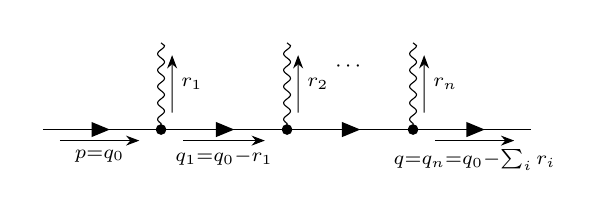
\begin{tikzpicture}[scale=0.8, transform shape, baseline={([yshift=0.2cm]current bounding box.center)}]
    \begin{feynman}
        

        \vertex (a) {};
        \vertex [dot, right=2cm of a] (b) {};
        \vertex [dot, right=2cm of b] (c) {};
        \vertex [dot, right=2cm of c] (d) {};
        \vertex [right=2cm of d] (e) {};

        \vertex[above=1.5 cm of b] (r1) {};
        \vertex[above=1.5 cm of c] (r2) {};
        \vertex [above=1.5 cm of d] (rn) {};
        

        \diagram*{

            (a) -- [fermion, momentum'={[arrow distance=4pt]\ensuremath{\scriptstyle p = q_0}}] (b) -- [fermion, momentum'={[arrow distance=4pt]\ensuremath{\scriptstyle q_1 = q_0 - r_1}}] (c) -- [fermion] (d) -- [fermion, momentum'={[arrow distance=4pt]\ensuremath{\scriptstyle q = q_n = q_0 - \sum_ir_i}}] (e), (b) -- [photon, momentum'={[arrow distance=4pt]\ensuremath{\scriptstyle r_1}}] (r1), (c) -- [photon, momentum'={[arrow distance=4pt]\ensuremath{\scriptstyle r_2}}] (r2), (d) -- [photon, momentum'={[arrow distance=4pt]\ensuremath{\scriptstyle r_n}}] (rn),

        };

         \node at ($(r2)!0.5!(rn)+(0,-0.5)$) {$\cdots$};

    \end{feynman}
\end{tikzpicture}.
\end{equation}
We then add an insertion of a new photon with momentum $k^\mu$ denoted as
\begin{equation}
    \slk = 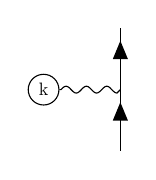
\begin{tikzpicture}[scale=0.65, transform shape, baseline={([yshift=-0.1cm]current bounding box.center)}]
    \begin{feynman}
        
        \vertex [draw,circle,minimum size=0.6cm,inner sep=0pt] (k) {k};
        \vertex [right=1.5cm of k] (right);
        \vertex [above right=1.2cm and 1.5cm of k] (up);
        \vertex [below right=1.2cm and 1.5cm of k] (down);

        \diagram*{
            (k) -- [photon] (right), (up) -- [anti fermion] (right) -- [anti fermion] (down)
        };

    \end{feynman}
    \end{tikzpicture}.
\end{equation}
If we make the insertion between photons $i$ and $i+1$ we will see 
\begin{equation}
\begin{aligned}
    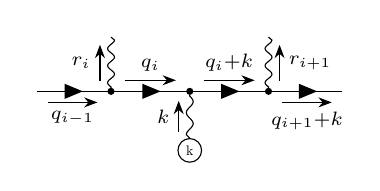
\begin{tikzpicture}[scale=0.5, transform shape, baseline={([yshift=-0.2cm]current bounding box.center)}]
    \begin{feynman}
        

        \vertex (a) {};
        \vertex [dot, right=2cm of a] (b) {};
        \vertex [dot, right=2cm of b] (c) {};
        \vertex [dot, right=2cm of c] (d) {};
        \vertex [right=2cm of d] (e) {};

        \vertex [above=1.5 cm of b] (r1) {};
        \vertex [below=1.5 cm of c, draw,circle,minimum size=0.6cm,inner sep=0pt] (r2) {k};
        \vertex [above=1.5 cm of d] (rn) {};
        

        \diagram*{

            (a) -- [fermion, momentum'={[arrow distance=4pt]\ensuremath{\scriptstyle q_{i-1}}}] (b) -- [fermion, momentum={[arrow distance=4pt]\ensuremath{\scriptstyle q_i}}] (c) -- [fermion, momentum={[arrow distance=4pt]\ensuremath{\scriptstyle q_i + k}}] (d) -- [fermion, momentum'={[arrow distance=4pt]\ensuremath{\scriptstyle q_{i+1} + k}}] (e),
            (b) -- [photon, momentum={[arrow distance=4pt]\ensuremath{\scriptstyle r_i}}] (r1), (c) -- [photon, reversed momentum'={[arrow distance=4pt]\ensuremath{\scriptstyle k}}] (r2), (d) -- [photon, momentum'={[arrow distance=4pt]\ensuremath{\scriptstyle r_{i+1}}}] (rn),

        };

    \end{feynman}
    \end{tikzpicture} &= \gamma^{\mu_i}\frac{\slq_i + m}{q_i^2 - m^2}\slk\frac{\slq_i + \slk + m}{(q_i + k)^2 - m^2}\gamma^{\mu_{i+1}} \\
    &= \gamma^{\mu_i}\bigg(\frac{\slq_i + m}{q_i^2 - m^2} - \frac{\slq_i + \slk + m}{(q_i + k)^2 - m^2}\bigg)\gamma^{\mu_{i+1}} \\
    &= 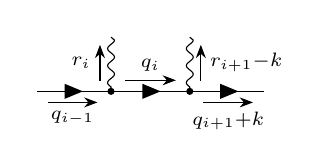
\begin{tikzpicture}[scale=0.5, transform shape, baseline={([yshift=-0.2cm]current bounding box.center)}]
    \begin{feynman}
        

        \vertex (a) {};
        \vertex [dot, right=2cm of a] (b) {};
        \vertex [dot, right=2cm of b] (c) {};
        \vertex [right=2cm of c] (d) {};

        \vertex [above=1.5 cm of b] (r1) {};
        \vertex [above=1.5 cm of c] (rn) {};
        

        \diagram*{

            (a) -- [fermion, momentum'={[arrow distance=4pt]\ensuremath{\scriptstyle q_{i-1}}}] (b) -- [fermion, momentum={[arrow distance=4pt]\ensuremath{\scriptstyle q_i}}] (c) -- [fermion, momentum'={[arrow distance=4pt]\ensuremath{\scriptstyle q_{i+1} + k}}] (d),
            
            (b) -- [photon, momentum={[arrow distance=4pt]\ensuremath{\scriptstyle r_i}}] (r1), (c) -- [photon, momentum'={[arrow distance=4pt]\ensuremath{\scriptstyle r_{i+1} - k}}] (rn),

        };

    \end{feynman}
    \end{tikzpicture} - 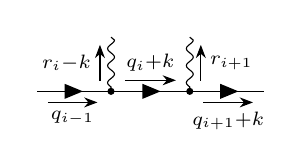
\begin{tikzpicture}[scale=0.5, transform shape, baseline={([yshift=-0.2cm]current bounding box.center)}]
    \begin{feynman}
        

        \vertex (a) {};
        \vertex [dot, right=2cm of a] (b) {};
        \vertex [dot, right=2cm of b] (c) {};
        \vertex [right=2cm of c] (d) {};

        \vertex [above=1.5 cm of b] (r1) {};
        \vertex [above=1.5 cm of c] (rn) {};
        

        \diagram*{

            (a) -- [fermion, momentum'={[arrow distance=4pt]\ensuremath{\scriptstyle q_{i-1}}}] (b) -- [fermion, momentum={[arrow distance=4pt]\ensuremath{\scriptstyle q_i + k}}] (c) -- [fermion, momentum'={[arrow distance=4pt]\ensuremath{\scriptstyle q_{i+1} + k}}] (d),
            
            (b) -- [photon, momentum={[arrow distance=4pt]\ensuremath{\scriptstyle r_i - k}}] (r1), (c) -- [photon, momentum'={[arrow distance=4pt]\ensuremath{\scriptstyle r_{i+1}}}] (rn),

        };

    \end{feynman}
    \end{tikzpicture},
\end{aligned}
\end{equation}
where we used $\slk = (\slq_i + \slk -m) - (\slq_i - m)$. Thus, using a shorthand notation
\begin{equation}
    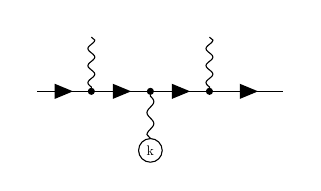
\begin{tikzpicture}[scale=0.5, transform shape, baseline={([yshift=-0.1cm]current bounding box.center)}]
    \begin{feynman}
        

        \vertex (a) {};
        \vertex [dot, right=1.5cm of a] (b) {};
        \vertex [dot, right=1.5cm of b] (c) {};
        \vertex [dot, right=1.5cm of c] (d) {};
        \vertex [right=2cm of d] (e) {};

        \vertex [above=1.5 cm of b] (r1) {};
        \vertex [below=1.5 cm of c, draw,circle,minimum size=0.6cm,inner sep=0pt] (r2) {k};
        \vertex [above=1.5 cm of d] (rn) {};
        

        \diagram*{

            (a) -- [fermion] (b) -- [fermion] (c) -- [fermion] (d) -- [fermion] (e),
            (b) -- [photon] (r1), (c) -- [photon] (r2), (d) -- [photon] (rn),

        };

    \end{feynman}
    \end{tikzpicture} = 
    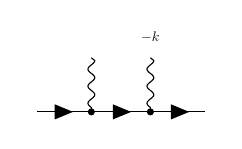
\begin{tikzpicture}[scale=0.5, transform shape, baseline={([yshift=-0.6cm]current bounding box.center)}]
    \begin{feynman}
        

        \vertex (a) {};
        \vertex [dot, right=1.5cm of a] (b) {};
        \vertex [dot, right=1.5cm of b] (c) {};
        \vertex [right=1.5cm of c] (d) {};

        \vertex [above=1.5 cm of b] (r1) {};
        \vertex [above=1.5 cm of c, label=\ensuremath{-k}] (rn) {};
        

        \diagram*{

            (a) -- [fermion] (b) -- [fermion] (c) -- [fermion] (d),
            
            (b) -- [photon] (r1), (c) -- [photon] (rn),

        };

    \end{feynman}
    \end{tikzpicture} - 
    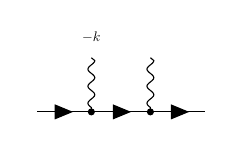
\begin{tikzpicture}[scale=0.5, transform shape, baseline={([yshift=-0.6cm]current bounding box.center)}]
    \begin{feynman}
        

        \vertex (a) {};
        \vertex [dot, right=1.5cm of a] (b) {};
        \vertex [dot, right=1.5cm of b] (c) {};
        \vertex [right=1.5cm of c] (d) {};

        \vertex [above=1.5 cm of b, label=\ensuremath{-k}] (r1) {};
        \vertex [above=1.5 cm of c] (rn) {};
        

        \diagram*{

            (a) -- [fermion] (b) -- [fermion] (c) -- [fermion] (d),
            (b) -- [photon] (r1), (c) -- [photon] (rn),

        };

    \end{feynman}
    \end{tikzpicture},
\end{equation}
we can sum insertions on adjacent propagators, so we get the following sum $S$ as
\begin{equation}
\begin{aligned}
    S &\equiv 
    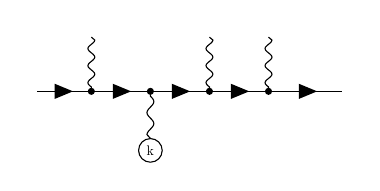
\begin{tikzpicture}[scale=0.5, transform shape, baseline={([yshift=-0.1cm]current bounding box.center)}]
    \begin{feynman}
        

        \vertex (a) {};
        \vertex [dot, right=1.5cm of a] (b) {};
        \vertex [dot, right=1.5cm of b] (c) {};
        \vertex [dot, right=1.5cm of c] (d) {};
        \vertex [dot, right=1.5cm of d] (e) {};
        \vertex [right=2cm of e] (f) {};

        \vertex [above=1.5 cm of b] (r1) {};
        \vertex [below=1.5 cm of c, draw,circle,minimum size=0.6cm,inner sep=0pt] (r2) {k};
        \vertex [above=1.5 cm of d] (r3) {};
        \vertex [above=1.5 cm of e] (r4) {};

        \diagram*{

            (a) -- [fermion] (b) -- [fermion] (c) -- [fermion] (d) -- [fermion] (e) -- [fermion] (f),
            (b) -- [photon] (r1), (c) -- [photon] (r2), (d) -- [photon] (r3), (e) -- [photon] (r4)

        };

    \end{feynman}
    \end{tikzpicture} +
    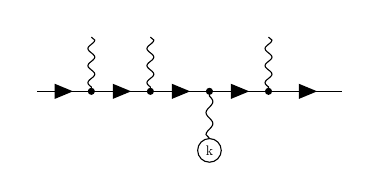
\begin{tikzpicture}[scale=0.5, transform shape, baseline={([yshift=-0.1cm]current bounding box.center)}]
    \begin{feynman}
        

        \vertex (a) {};
        \vertex [dot, right=1.5cm of a] (b) {};
        \vertex [dot, right=1.5cm of b] (c) {};
        \vertex [dot, right=1.5cm of c] (d) {};
        \vertex [dot, right=1.5cm of d] (e) {};
        \vertex [right=2cm of e] (f) {};

        \vertex [above=1.5 cm of b] (r1) {};
        \vertex [below=1.5 cm of d, draw,circle,minimum size=0.6cm,inner sep=0pt] (r2) {k};
        \vertex [above=1.5 cm of c] (r3) {};
        \vertex [above=1.5 cm of e] (r4) {};

        \diagram*{

            (a) -- [fermion] (b) -- [fermion] (c) -- [fermion] (d) -- [fermion] (e) -- [fermion] (f),
            (b) -- [photon] (r1), (c) -- [photon] (r3), (d) -- [photon] (r2), (e) -- [photon] (r4)

        };

    \end{feynman}
    \end{tikzpicture}\\
    &= 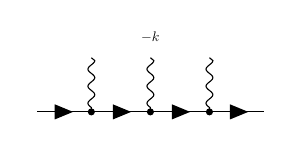
\begin{tikzpicture}[scale=0.5, transform shape, baseline={([yshift=-0.6cm]current bounding box.center)}]
    \begin{feynman}
        

        \vertex (a) {};
        \vertex [dot, right=1.5cm of a] (b) {};
        \vertex [dot, right=1.5cm of b] (c) {};
        \vertex [dot, right=1.5cm of c] (d) {};
        \vertex [right=1.5cm of d] (e) {};

        \vertex [above=1.5 cm of b] (r1) {};
        \vertex [above=1.5 cm of c, label=\ensuremath{-k}] (r2) {};
        \vertex [above=1.5 cm of d] (r3) {};
    
        \diagram*{

            (a) -- [fermion] (b) -- [fermion] (c) -- [fermion] (d) -- [fermion] (e),
            (b) -- [photon] (r1), (c) -- [photon] (r2), (d) -- [photon] (r3)

        };

    \end{feynman}
    \end{tikzpicture} - 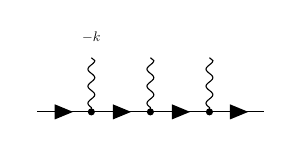
\begin{tikzpicture}[scale=0.5, transform shape, baseline={([yshift=-0.6cm]current bounding box.center)}]
    \begin{feynman}
        

        \vertex (a) {};
        \vertex [dot, right=1.5cm of a] (b) {};
        \vertex [dot, right=1.5cm of b] (c) {};
        \vertex [dot, right=1.5cm of c] (d) {};
        \vertex [right=1.5cm of d] (e) {};

        \vertex [above=1.5 cm of b, label=\ensuremath{-k}] (r1) {};
        \vertex [above=1.5 cm of c] (r2) {};
        \vertex [above=1.5 cm of d] (r3) {};
    
        \diagram*{

            (a) -- [fermion] (b) -- [fermion] (c) -- [fermion] (d) -- [fermion] (e),
            (b) -- [photon] (r1), (c) -- [photon] (r2), (d) -- [photon] (r3)

        };

    \end{feynman}
    \end{tikzpicture} \\
    &+ 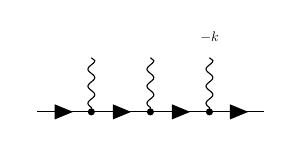
\begin{tikzpicture}[scale=0.5, transform shape, baseline={([yshift=-0.6cm]current bounding box.center)}]
    \begin{feynman}
        

        \vertex (a) {};
        \vertex [dot, right=1.5cm of a] (b) {};
        \vertex [dot, right=1.5cm of b] (c) {};
        \vertex [dot, right=1.5cm of c] (d) {};
        \vertex [right=1.5cm of d] (e) {};

        \vertex [above=1.5 cm of b] (r1) {};
        \vertex [above=1.5 cm of c] (r2) {};
        \vertex [above=1.5 cm of d, label=\ensuremath{-k}] (r3) {};
    
        \diagram*{

            (a) -- [fermion] (b) -- [fermion] (c) -- [fermion] (d) -- [fermion] (e),
            (b) -- [photon] (r1), (c) -- [photon] (r2), (d) -- [photon] (r3)

        };

    \end{feynman}
    \end{tikzpicture} - 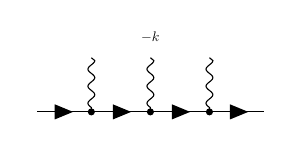
\begin{tikzpicture}[scale=0.5, transform shape, baseline={([yshift=-0.6cm]current bounding box.center)}]
    \begin{feynman}
        

        \vertex (a) {};
        \vertex [dot, right=1.5cm of a] (b) {};
        \vertex [dot, right=1.5cm of b] (c) {};
        \vertex [dot, right=1.5cm of c] (d) {};
        \vertex [right=1.5cm of d] (e) {};

        \vertex [above=1.5 cm of b] (r1) {};
        \vertex [above=1.5 cm of c, label=\ensuremath{-k}] (r2) {};
        \vertex [above=1.5 cm of d] (r3) {};
    
        \diagram*{

            (a) -- [fermion] (b) -- [fermion] (c) -- [fermion] (d) -- [fermion] (e),
            (b) -- [photon] (r1), (c) -- [photon] (r2), (d) -- [photon] (r3)

        };

    \end{feynman}
    \end{tikzpicture} \\
    &= 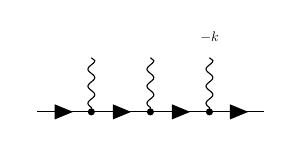
\begin{tikzpicture}[scale=0.5, transform shape, baseline={([yshift=-0.6cm]current bounding box.center)}]
    \begin{feynman}
        

        \vertex (a) {};
        \vertex [dot, right=1.5cm of a] (b) {};
        \vertex [dot, right=1.5cm of b] (c) {};
        \vertex [dot, right=1.5cm of c] (d) {};
        \vertex [right=1.5cm of d] (e) {};

        \vertex [above=1.5 cm of b] (r1) {};
        \vertex [above=1.5 cm of c] (r2) {};
        \vertex [above=1.5 cm of d, label=\ensuremath{-k}] (r3) {};
    
        \diagram*{

            (a) -- [fermion] (b) -- [fermion] (c) -- [fermion] (d) -- [fermion] (e),
            (b) -- [photon] (r1), (c) -- [photon] (r2), (d) -- [photon] (r3)

        };

    \end{feynman}
    \end{tikzpicture} - 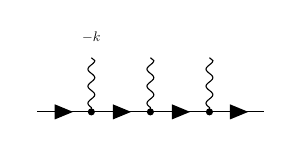
\begin{tikzpicture}[scale=0.5, transform shape, baseline={([yshift=-0.6cm]current bounding box.center)}]
    \begin{feynman}
        

        \vertex (a) {};
        \vertex [dot, right=1.5cm of a] (b) {};
        \vertex [dot, right=1.5cm of b] (c) {};
        \vertex [dot, right=1.5cm of c] (d) {};
        \vertex [right=1.5cm of d] (e) {};

        \vertex [above=1.5 cm of b, label=\ensuremath{-k}] (r1) {};
        \vertex [above=1.5 cm of c] (r2) {};
        \vertex [above=1.5 cm of d] (r3) {};
    
        \diagram*{

            (a) -- [fermion] (b) -- [fermion] (c) -- [fermion] (d) -- [fermion] (e),
            (b) -- [photon] (r1), (c) -- [photon] (r2), (d) -- [photon] (r3)

        };

    \end{feynman}
    \end{tikzpicture},
    \end{aligned}
\end{equation}
and also compute the following product $P$, summing over all insertions, as
\begin{equation}
    \begin{aligned}
        P &= 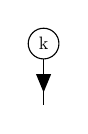
\begin{tikzpicture}[scale=0.65, transform shape, baseline={([yshift=-0.2cm]current bounding box.center)}]
    \begin{feynman}
        
        \vertex [draw,circle,minimum size=0.6cm,inner sep=0pt] (k) {k};
        \vertex [below=1.2cm of k] (down);

        \diagram*{

            (k) -- [fermion] (down),
        };

    \end{feynman}
\end{tikzpicture} \otimes
    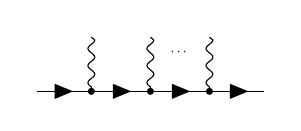
\begin{tikzpicture}[scale=0.5, transform shape, baseline={([yshift=-0.5cm]current bounding box.center)}]
    \begin{feynman}
        

        \vertex (a) {};
        \vertex [dot, right=1.5cm of a] (b) {};
        \vertex [dot, right=1.5cm of b] (c) {};
        \vertex [dot, right=1.5cm of c] (d) {};
        \vertex [right=1.5cm of d] (e) {};

        \vertex[above=1.5 cm of b] (r1) {};
        \vertex[above=1.5 cm of c] (r2) {};
        \vertex[above=1.5 cm of d] (rn) {};
        

        \diagram*{

            (a) -- [fermion] (b) -- [fermion] (c) -- [fermion] (d) -- [fermion] (e), (b) -- [photon] (r1), (c) -- [photon] (r2), (d) -- [photon] (rn),

        };

         \node at ($(r2)!0.5!(rn)+(0,-0.5)$) {$\cdots$};

    \end{feynman}
    \end{tikzpicture} \\
    &= 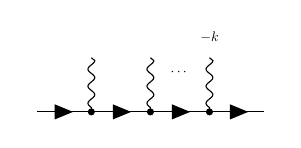
\begin{tikzpicture}[scale=0.5, transform shape, baseline={([yshift=-0.5cm]current bounding box.center)}]
    \begin{feynman}
        

        \vertex (a) {};
        \vertex [dot, right=1.5cm of a] (b) {};
        \vertex [dot, right=1.5cm of b] (c) {};
        \vertex [dot, right=1.5cm of c] (d) {};
        \vertex [right=1.5cm of d] (e) {};

        \vertex[above=1.5 cm of b] (r1) {};
        \vertex[above=1.5 cm of c] (r2) {};
        \vertex [above=1.5 cm of d, label=\ensuremath{-k}] (rn) {};
        

        \diagram*{

            (a) -- [fermion] (b) -- [fermion] (c) -- [fermion] (d) -- [fermion] (e), (b) -- [photon] (r1), (c) -- [photon] (r2), (d) -- [photon] (rn),

        };

         \node at ($(r2)!0.5!(rn)+(0,-0.5)$) {$\cdots$};

    \end{feynman}
    \end{tikzpicture} - 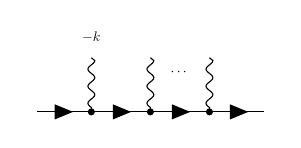
\begin{tikzpicture}[scale=0.5, transform shape, baseline={([yshift=-0.5cm]current bounding box.center)}]
    \begin{feynman}
        

        \vertex (a) {};
        \vertex [dot, right=1.5cm of a] (b) {};
        \vertex [dot, right=1.5cm of b] (c) {};
        \vertex [dot, right=1.5cm of c] (d) {};
        \vertex [right=1.5cm of d] (e) {};

        \vertex[above=1.5 cm of b, label=\ensuremath{-k}] (r1) {};
        \vertex[above=1.5 cm of c] (r2) {};
        \vertex [above=1.5 cm of d] (rn) {};
        

        \diagram*{

            (a) -- [fermion] (b) -- [fermion] (c) -- [fermion] (d) -- [fermion] (e), (b) -- [photon] (r1), (c) -- [photon] (r2), (d) -- [photon] (rn),

        };

         \node at ($(r2)!0.5!(rn)+(0,-0.5)$) {$\cdots$};

    \end{feynman}
    \end{tikzpicture} \\
    &+ 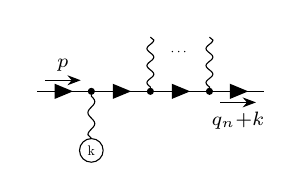
\begin{tikzpicture}[scale=0.5, transform shape, baseline={([yshift=0.2cm]current bounding box.center)}]
    \begin{feynman}
        

        \vertex (a) {};
        \vertex [dot, right=1.5cm of a] (b) {};
        \vertex [dot, right=1.5cm of b] (c) {};
        \vertex [dot, right=1.5cm of c] (d) {};
        \vertex [right=1.5cm of d] (e) {};

        \vertex[below=1.5 cm of b,draw,circle,minimum size=0.6cm,inner sep=0pt] (r1) {k};
        \vertex[above=1.5 cm of c] (r2) {};
        \vertex [above=1.5 cm of d] (rn) {};
        

        \diagram*{

            (a) -- [fermion, momentum={[arrow distance=4pt]\ensuremath{\scriptstyle p}}] (b) -- [fermion] (c) -- [fermion] (d) -- [fermion, momentum'={[arrow distance=4pt]\ensuremath{\scriptstyle q_n + k}}] (e), (b) -- [photon] (r1), (c) -- [photon] (r2), (d) -- [photon] (rn),

        };

         \node at ($(r2)!0.5!(rn)+(0,-0.5)$) {$\cdots$};

    \end{feynman}
    \end{tikzpicture} + 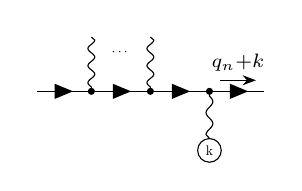
\begin{tikzpicture}[scale=0.5, transform shape, baseline={([yshift=0.2cm]current bounding box.center)}]
    \begin{feynman}
        

        \vertex (a) {};
        \vertex [dot, right=1.5cm of a] (b) {};
        \vertex [dot, right=1.5cm of b] (c) {};
        \vertex [dot, right=1.5cm of c] (d) {};
        \vertex [right=1.5cm of d] (e) {};

        \vertex[above=1.5 cm of b] (r1) {};
        \vertex[above=1.5 cm of c] (r2) {};
        \vertex [below=1.5 cm of d,draw,circle,minimum size=0.6cm,inner sep=0pt] (rn) {k};
        

        \diagram*{

            (a) -- [fermion] (b) -- [fermion] (c) -- [fermion] (d) -- [fermion, momentum={[arrow distance=4pt]\ensuremath{\scriptstyle q_n + k}}] (e), (b) -- [photon] (r1), (c) -- [photon] (r2), (d) -- [photon] (rn),

        };

         \node at ($(r1)!0.5!(r2)+(0,-0.5)$) {$\cdots$};

    \end{feynman}
    \end{tikzpicture}.
\end{aligned} 
\end{equation}
Also
\begin{equation}
    \begin{aligned}
        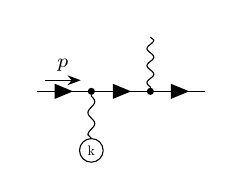
\begin{tikzpicture}[scale=0.5, transform shape, baseline={([yshift=-0.1cm]current bounding box.center)}]
    \begin{feynman}
        

        \vertex (a) {};
        \vertex [dot, right=1.5cm of a] (b) {};
        \vertex [dot, right=1.5cm of b] (c) {};
        \vertex [right=1.5cm of c] (d) {};

        \vertex [below=1.5 cm of b,draw,circle,minimum size=0.6cm,inner sep=0pt] (r1) {k};
        \vertex [above=1.5 cm of c] (rn) {};
        

        \diagram*{

            (a) -- [fermion, momentum={[arrow distance=4pt]\ensuremath{\scriptstyle p}}] (b) -- [fermion] (c) -- [fermion] (d),
            
            (b) -- [photon] (r1), (c) -- [photon] (rn),

        };

    \end{feynman}
    \end{tikzpicture} &= \frac{\slp + m}{p^2- m^2}\slk\frac{\slp + \slk + m}{(p + k)^2 - m^2} \\
        &= 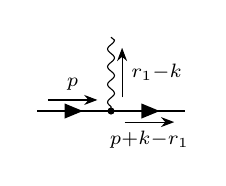
\begin{tikzpicture}[scale=0.5, transform shape, baseline={([yshift=-0.3cm]current bounding box.center)}]
    \begin{feynman}
        
        \vertex (a) {};
        \vertex [dot, right=2cm of a] (b) {};
        \vertex [right=2cm of b] (c) {};
        
        \vertex [above=2cm of b] (r1) {};

        \diagram*{

            (a) -- [fermion, momentum={[arrow distance=4pt]\ensuremath{\scriptstyle p}}] (b) -- [fermion, momentum'={[arrow distance=4pt]\ensuremath{\scriptstyle p + k - r_1 }}] (c),
            (b) -- [photon, momentum'={[arrow distance=4pt]\ensuremath{\scriptstyle r_1 - k}}] (r1)

        };

    \end{feynman}
    \end{tikzpicture} - 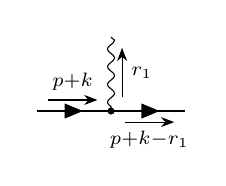
\begin{tikzpicture}[scale=0.5, transform shape, baseline={([yshift=-0.3cm]current bounding box.center)}]
    \begin{feynman}

        \vertex (a) {};
        \vertex [dot, right=2cm of a] (b) {};
        \vertex [right=2cm of b] (c) {};

        \vertex [above=2 cm of b] (r1) {};

        \diagram*{

            (a) -- [fermion, momentum={[arrow distance=4pt]\ensuremath{\scriptstyle p + k}}] (b) -- [fermion, momentum'={[arrow distance=4pt]\ensuremath{\scriptstyle p + k - r_1}}] (c),
            (b) -- [photon, momentum'={[arrow distance=4pt]\ensuremath{\scriptstyle r_1}}] (r1)

        };

    \end{feynman}
    \end{tikzpicture},
    \end{aligned}
\end{equation}
and 
\begin{equation}
    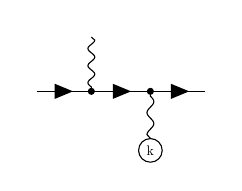
\begin{tikzpicture}[scale=0.5, transform shape, baseline={([yshift=-0.1cm]current bounding box.center)}]
    \begin{feynman}
        
        \vertex (a) {};
        \vertex [dot, right=1.5cm of a] (b) {};
        \vertex [dot, right=1.5cm of b] (c) {};
        \vertex [right=1.5cm of c] (d) {};

        \vertex [above=1.5 cm of b] (r1) {};
        \vertex [below=1.5 cm of c,draw,circle,minimum size=0.6cm,inner sep=0pt] (rn) {k};
        
        \diagram*{

            (a) -- [fermion] (b) -- [fermion] (c) -- [fermion] (d),
            
            (b) -- [photon] (r1), (c) -- [photon] (rn),

        };

    \end{feynman}
    \end{tikzpicture} = 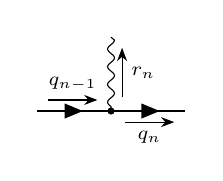
\begin{tikzpicture}[scale=0.5, transform shape, baseline={([yshift=-0.3cm]current bounding box.center)}]
    \begin{feynman}
        
        \vertex (a) {};
        \vertex [dot, right=2cm of a] (b) {};
        \vertex [right=2cm of b] (c) {};

        \vertex [above=2cm of b] (r1) {};

        \diagram*{

            (a) -- [fermion, momentum={[arrow distance=4pt]\ensuremath{\scriptstyle q_{n-1}}}] (b) -- [fermion, momentum'={[arrow distance=4pt]\ensuremath{\scriptstyle q_n}}] (c),
            (b) -- [photon, momentum'={[arrow distance=4pt]\ensuremath{\scriptstyle r_n}}] (r1)

        };

    \end{feynman}
    \end{tikzpicture} - 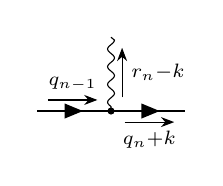
\begin{tikzpicture}[scale=0.5, transform shape, baseline={([yshift=-0.3cm]current bounding box.center)}]
    \begin{feynman}
        
        \vertex (a) {};
        \vertex [dot, right=2cm of a] (b) {};
        \vertex [right=2cm of b] (c) {};

        \vertex [above=2cm of b] (r1) {};

        \diagram*{

            (a) -- [fermion, momentum={[arrow distance=4pt]\ensuremath{\scriptstyle q_{n-1}}}] (b) -- [fermion, momentum'={[arrow distance=4pt]\ensuremath{\scriptstyle q_n + k}}] (c),
            (b) -- [photon, momentum'={[arrow distance=4pt]\ensuremath{\scriptstyle r_n - k}}] (r1)

        };

    \end{feynman}
    \end{tikzpicture},
\end{equation}
thus
\begin{equation}
\label{eq: sum over insertions on adjacent propagators}
    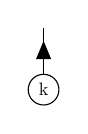
\begin{tikzpicture}[scale=0.65, transform shape, baseline={([yshift=-0.2cm]current bounding box.center)}]
    \begin{feynman}
        
        \vertex [draw,circle,minimum size=0.6cm,inner sep=0pt] (k) {k};
        \vertex [above=1.2cm of k] (down);

        \diagram*{

            (k) -- [fermion] (down),
        };

    \end{feynman}
\end{tikzpicture} \otimes
    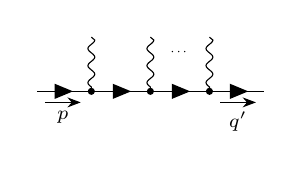
\begin{tikzpicture}[scale=0.5, transform shape, baseline={([yshift=-0.2cm]current bounding box.center)}]
    \begin{feynman}

        \vertex (a) {};
        \vertex [dot, right=1.5cm of a] (b) {};
        \vertex [dot, right=1.5cm of b] (c) {};
        \vertex [dot, right=1.5cm of c] (d) {};
        \vertex [right=1.5cm of d] (e) {};

        \vertex[above=1.5 cm of b] (r1) {};
        \vertex[above=1.5 cm of c] (r2) {};
        \vertex[above=1.5 cm of d] (rn) {};

        \diagram*{

            (a) -- [fermion, momentum'={[arrow distance=4pt]\ensuremath{\scriptstyle p}}] (b) -- [fermion] (c) -- [fermion] (d) -- [fermion, momentum'={[arrow distance=4pt]\ensuremath{\scriptstyle q'}}] (e), (b) -- [photon] (r1), (c) -- [photon] (r2), (d) -- [photon] (rn),

        };

         \node at ($(r2)!0.5!(rn)+(0,-0.5)$) {$\cdots$};

    \end{feynman}
    \end{tikzpicture}
    =
     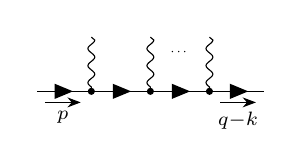
\begin{tikzpicture}[scale=0.5, transform shape, baseline={([yshift=-0.2cm]current bounding box.center)}]
    \begin{feynman}
        
        \vertex (a) {};
        \vertex [dot, right=1.5cm of a] (b) {};
        \vertex [dot, right=1.5cm of b] (c) {};
        \vertex [dot, right=1.5cm of c] (d) {};
        \vertex [right=1.5cm of d] (e) {};

        \vertex[above=1.5 cm of b] (r1) {};
        \vertex[above=1.5 cm of c] (r2) {};
        \vertex [above=1.5 cm of d] (rn) {};

        \diagram*{

            (a) -- [fermion, momentum'={[arrow distance=4pt]\ensuremath{\scriptstyle p}}] (b) -- [fermion] (c) -- [fermion] (d) -- [fermion, momentum'={[arrow distance=4pt]\ensuremath{\scriptstyle q - k}}] (e), (b) -- [photon] (r1), (c) -- [photon] (r2), (d) -- [photon] (rn),

        };

         \node at ($(r2)!0.5!(rn)+(0,-0.5)$) {$\cdots$};

    \end{feynman}
    \end{tikzpicture} - 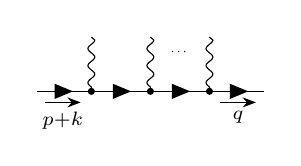
\begin{tikzpicture}[scale=0.5, transform shape, baseline={([yshift=-0.2cm]current bounding box.center)}]
    \begin{feynman}
        
        \vertex (a) {};
        \vertex [dot, right=1.5cm of a] (b) {};
        \vertex [dot, right=1.5cm of b] (c) {};
        \vertex [dot, right=1.5cm of c] (d) {};
        \vertex [right=1.5cm of d] (e) {};

        \vertex[above=1.5 cm of b] (r1) {};
        \vertex[above=1.5 cm of c] (r2) {};
        \vertex [above=1.5 cm of d] (rn) {};
        
        \diagram*{

            (a) -- [fermion, momentum'={[arrow distance=4pt]\ensuremath{\scriptstyle p + k}}] (b) -- [fermion] (c) -- [fermion] (d) -- [fermion, momentum'={[arrow distance=4pt]\ensuremath{\scriptstyle q}}] (e), (b) -- [photon] (r1), (c) -- [photon] (r2), (d) -- [photon] (rn),

        };

         \node at ($(r2)!0.5!(rn)+(0,-0.5)$) {$\cdots$};

    \end{feynman}
    \end{tikzpicture}
\end{equation}
where $q \equiv p + k -\sum_ir_i$ and $q' \equiv p - \sum_ir_i$. \begin{obs}
    Note that if we apply the LSZ formalism to the correlation function and put the external legs on-shell, the two terms cancel recovering the Ward identity.
\end{obs} 
The relation is valid off-shell so applies to any sub-diagram. To complete the proof we must consider insertions on internal, closed loop, fermion lines. A closed loop with $n$-photons attached is written as
\begin{equation}
    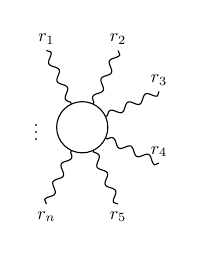
\begin{tikzpicture}[scale=0.65, transform shape, baseline={([yshift=-0.1cm]current bounding box.center)}]
    \begin{feynman}
        
        \vertex [draw,circle,minimum size=1cm,inner sep=0pt] (v) {};

        \vertex [above left=1.5cm and 0.7cm of v, label=\ensuremath{ r_1}] (q1);
        \vertex [above right=1.5cm and 0.7cm of v, label=\ensuremath{ r_2}] (qn);

        % p
        \vertex [below left=1.5cm and 0.7cm of v, label={[label distance=0.5pt]below:\ensuremath{r_n}}] (p1);
        \vertex [below right=1.5cm and 0.7cm of v, label={[label distance=0.5pt]below:\ensuremath{r_5}}] (pn);

        % r
        \vertex [above right=0.7 and 1.5cm of v, label=\ensuremath{ r_3}] (r1);
        \vertex [below right=0.7 and 1.5cm of v, label=\ensuremath{ r_4}] (rn);

        \diagram*{

            (v) -- [photon] (q1),
            (v) -- [photon] (qn),

            (v) -- [photon] (p1),
            (v) -- [photon] (pn),

            (v) -- [photon] (r1),
            (v) -- [photon] (rn)
        };
 
         \node at ($(q1)!0.5!(p1)+(-0.2,0)$) {$\vdots$};

    \end{feynman}
\end{tikzpicture} = \bigtr{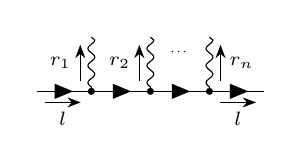
\begin{tikzpicture}[scale=0.5, transform shape, baseline={([yshift=-0.1cm]current bounding box.center)}]
    \begin{feynman}
        

        \vertex (a) {};
        \vertex [dot, right=1.5cm of a] (b) {};
        \vertex [dot, right=1.5cm of b] (c) {};
        \vertex [dot, right=1.5cm of c] (d) {};
        \vertex [right=1.5cm of d] (e) {};

        \vertex[above=1.5 cm of b] (r1) {};
        \vertex[above=1.5 cm of c] (r2) {};
        \vertex[above=1.5 cm of d] (rn) {};
        

        \diagram*{

            (a) -- [fermion, momentum'={[arrow distance=4pt]\ensuremath{\scriptstyle l}}] (b) -- [fermion] (c) -- [fermion] (d) -- [fermion, momentum'={[arrow distance=4pt]\ensuremath{\scriptstyle l}}] (e), (b) -- [photon, momentum={[arrow distance=4pt]\ensuremath{\scriptstyle r_1}}] (r1), (c) -- [photon, momentum={[arrow distance=4pt]\ensuremath{\scriptstyle r_2}}] (r2), (d) -- [photon, momentum'={[arrow distance=4pt]\ensuremath{\scriptstyle r_n}}] (rn),

        };

         \node at ($(r2)!0.5!(rn)+(0,-0.5)$) {$\cdots$};

    \end{feynman}
    \end{tikzpicture}},
\end{equation}
where $r_i$ are outgoing photon and $l$ is an internal loop momentum. On the left-hand side we have used the notation $\nparallel$ to indicate the end-points are the same. When we sum over all insertion points, we can use the same type of relations as before and only the changed momentum conservation conditions results in the final two contributions cancelling
\begin{equation}
\label{eq: sum over insertion points}
\begin{aligned}
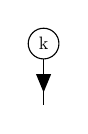
\begin{tikzpicture}[scale=0.65, transform shape, baseline={([yshift=0.2cm]current bounding box.center)}]
    \begin{feynman}
        
        \vertex [draw,circle,minimum size=0.6cm,inner sep=0pt] (k) {k};
        \vertex [below=1.2cm of k] (down);

        \diagram*{

            (k) -- [fermion] (down),
        };

    \end{feynman}
\end{tikzpicture} \otimes
    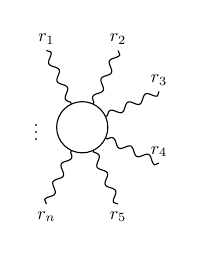
\begin{tikzpicture}[scale=0.65, transform shape, baseline={([yshift=-0.1cm]current bounding box.center)}]
    \begin{feynman}
        
        \vertex [draw,circle,minimum size=1cm,inner sep=0pt] (v) {};

        \vertex [above left=1.5cm and 0.7cm of v, label=\ensuremath{ r_1}] (q1);
        \vertex [above right=1.5cm and 0.7cm of v, label=\ensuremath{ r_2}] (qn);

        % p
        \vertex [below left=1.5cm and 0.7cm of v, label={[label distance=0.5pt]below:\ensuremath{r_n}}] (p1);
        \vertex [below right=1.5cm and 0.7cm of v, label={[label distance=0.5pt]below:\ensuremath{r_5}}] (pn);

        % r
        \vertex [above right=0.7 and 1.5cm of v, label=\ensuremath{ r_3}] (r1);
        \vertex [below right=0.7 and 1.5cm of v, label=\ensuremath{ r_4}] (rn);

        \diagram*{

            (v) -- [photon] (q1),
            (v) -- [photon] (qn),

            (v) -- [photon] (p1),
            (v) -- [photon] (pn),

            (v) -- [photon] (r1),
            (v) -- [photon] (rn)
        };
 
         \node at ($(q1)!0.5!(p1)+(-0.2,0)$) {$\vdots$};

    \end{feynman}
\end{tikzpicture} &= \bigtr{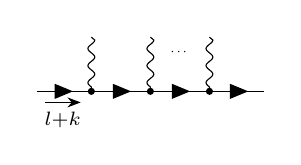
\begin{tikzpicture}[scale=0.5, transform shape, baseline={([yshift=-0.1cm]current bounding box.center)}]
    \begin{feynman}
        

        \vertex (a) {};
        \vertex [dot, right=1.5cm of a] (b) {};
        \vertex [dot, right=1.5cm of b] (c) {};
        \vertex [dot, right=1.5cm of c] (d) {};
        \vertex [right=1.5cm of d] (e) {};

        \vertex[above=1.5 cm of b] (r1) {};
        \vertex[above=1.5 cm of c] (r2) {};
        \vertex[above=1.5 cm of d] (rn) {};
        

        \diagram*{

            (a) -- [fermion, momentum'={[arrow distance=4pt]\ensuremath{\scriptstyle l + k}}] (b) -- [fermion] (c) -- [fermion] (d) -- [fermion] (e), (b) -- [photon] (r1), (c) -- [photon] (r2), (d) -- [photon,] (rn),

        };

         \node at ($(r2)!0.5!(rn)+(0,-0.5)$) {$\cdots$};

    \end{feynman}
    \end{tikzpicture}} - \bigtr{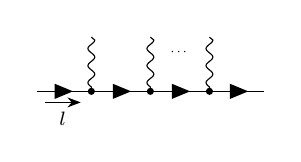
\begin{tikzpicture}[scale=0.5, transform shape, baseline={([yshift=-0.1cm]current bounding box.center)}]
    \begin{feynman}
        

        \vertex (a) {};
        \vertex [dot, right=1.5cm of a] (b) {};
        \vertex [dot, right=1.5cm of b] (c) {};
        \vertex [dot, right=1.5cm of c] (d) {};
        \vertex [right=1.5cm of d] (e) {};

        \vertex[above=1.5 cm of b] (r1) {};
        \vertex[above=1.5 cm of c] (r2) {};
        \vertex[above=1.5 cm of d] (rn) {};
        

        \diagram*{

            (a) -- [fermion, momentum'={[arrow distance=4pt]\ensuremath{\scriptstyle l}}] (b) -- [fermion] (c) -- [fermion] (d) -- [fermion] (e), (b) -- [photon] (r1), (c) -- [photon] (r2), (d) -- [photon] (rn),

        };

         \node at ($(r2)!0.5!(rn)+(0,-0.5)$) {$\cdots$};

    \end{feynman}
    \end{tikzpicture}} \\
    &= 0.
\end{aligned}
\end{equation}
The two equations \eqref{eq: sum over insertions on adjacent propagators} and \eqref{eq: sum over insertion points} are sufficient to prove the general relation. It is interesting to consider a special case of the Ward-Takahashi identity for the 2-point electron self-energy
\begin{equation}
    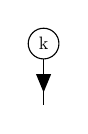
\begin{tikzpicture}[scale=0.65, transform shape, baseline={([yshift=0.2cm]current bounding box.center)}]
    \begin{feynman}
        
        \vertex [draw,circle,minimum size=0.6cm,inner sep=0pt] (k) {k};
        \vertex [below=1.2cm of k] (down);

        \diagram*{

            (k) -- [fermion] (down),
        };

    \end{feynman}
    \end{tikzpicture} \otimes 
    \feynmandiagram[inline=(v.base), layered layout, horizontal=a to b, scale=0.8, transform shape] { 
        a -- [fermion, momentum'={[arrow distance = 5pt]\(\scriptstyle p\)},] v [blob, pos=0.5] -- [fermion] b, 
        }; = e_R(\feynmandiagram[inline=(v.base), layered layout, horizontal=a to b, scale=0.8, transform shape] { 
        a -- [fermion, momentum'={[arrow distance = 5pt]\(\scriptstyle p\)}] v [blob, pos=0.5] -- [fermion] b, 
        }; - \feynmandiagram[inline=(v.base), layered layout, horizontal=a to b, scale=0.8, transform shape] { 
        a -- [fermion, momentum'={[arrow distance = 5pt]\(\scriptstyle p + k\)}] v [blob, pos=0.5] -- [fermion] b, 
        };) = \feynmandiagram[inline={([yshift=-0.2cm]current bounding box.center)}, scale = 0.9, horizontal=a to c] { 
    a -- [fermion, momentum'={[arrow distance=4pt] \ensuremath{\scriptstyle p}}] b [blob] -- [photon, reversed momentum={[arrow distance=4pt] \ensuremath{\scriptstyle k}}, label=\ensuremath{\scriptstyle A_c^\mu}] d, b -- [fermion, momentum={[arrow distance=4pt] \ensuremath{\scriptstyle p + k}}] c};k_\mu.
\end{equation}
The 2-point function is
\begin{equation}
    \feynmandiagram[inline=(v.base), layered layout, horizontal=a to b, scale=0.8, transform shape] { 
        a -- [fermion, momentum'={[arrow distance = 5pt]\(\scriptstyle p\)},] v [blob, pos=0.5] -- [fermion] b, 
        }; = \frac{i}{\slp - m_R - \Sigma_R(p,m_R)} = S(p),
\end{equation}
while the vertex function appears on the left-hand side as
\begin{equation}
    \feynmandiagram[inline={([yshift=-0.2cm]current bounding box.center)}, scale = 0.9, horizontal=a to c] { 
    a -- [fermion, momentum'={[arrow distance=4pt] \ensuremath{\scriptstyle p}}] b [blob] -- [photon, reversed momentum={[arrow distance=4pt] \ensuremath{\scriptstyle k}}, label=\ensuremath{\scriptstyle A_c^\mu}] d, b -- [fermion, momentum={[arrow distance=4pt] \ensuremath{\scriptstyle p + k}}] c};k_\mu = S(p)[-ie_R\Gamma_R^\mu(p,p + k)k_\mu]S(p + k).
\end{equation}
Multiplying the inverse propagator leads to the relation 
\begin{equation}
    -ik_\mu\Gamma_R^\mu(p,p + k) = S^{-1}(p + k) - S^{-1}(p),
\end{equation}
as we take the limit for $k \to 0$ we identify the renormalization constants $Z_1$ and $Z_\psi$ with
\begin{equation}
    \lim_{k \to 0}\Gamma_R^\mu(p,p + k) = Z_1^{-1}\gamma^\mu, \quad S(p) = \frac{iZ_\psi}{\slp - m_R} + o(\slp - m_R),
\end{equation}
hence
\begin{equation}
    -i\slk Z_1^{-1} = -i(\slp + \slk)Z_\psi^{-1} - (-i\slp)Z_\psi^{-1},
\end{equation}
resulting in 
\begin{equation}
    Z_1 = Z_\psi.
\end{equation}
So the Ward-Takahashi identity is directly connected with the gauge invariance constraint that identifies $Z_1$ with $Z_\psi$. 
% \chapter{QCD at 1-loop}
We will consider a $SU(n_c)$ gauge theory with $n_f$ quark flavours transforming in the fundamental representation. The gluon field $A_\mu^a$ is quantized in a covariant gauge using the Faddeev-Popov method which introduces the ghost fields $c^a$. The complete field content is constituted by $\psi_{q\alpha i}$, $A^{\mu a}$ and $c^a$, where the indices are $q = 1,\dots,n_f$ for the flavours, $\alpha = 1,\dots,4$ for the spinors, $a = 1, \dots, n_c^2 - 1 $ for the colour of $A^\mu$ and $c$, $i = 1, \dots, n_c$ for the colour of $\psi$, and $\mu = 0,\dots,3$ for the Lorentz quantities. The bare Lagrangian is
\begin{equation}
    \begin{split}
        \dL_{QCD,0} &= -\frac{1}{4}F_0^{\mu\nu a}F^a_{0\mu\nu} + \sum_{q=1}^{n_f}\psib_{0q\alpha i}(i\slD_0 - m_{0q})_{ij\alpha\beta}\psi_{0q\beta j} \\
        &- \frac{1}{2\xi}(\p_\mu A^{\mu a}_0)(\p_\nu A^{\nu a}_0) + \p^\mu\cbar^a_0D^{ab}_{0\mu}c^b_0,
    \end{split}
\end{equation}
where 
\begin{align}
    F_0^{\mu\nu a} = \p^\mu A^{\nu a}_0 - \p^\nu A^{\mu a}_0 - g_{S0}f^{abc}A_0^{\mu b}A^{\nu c}_0,\quad \slD_{0ij\alpha\beta} = \gamma^\mu_{\alpha\beta}D_{0\mu ij}, \\
    D^\mu_{0ij} = \p^\mu\delta_{ij} - ig_{S0}t^a_{ij}A^{\mu a}_0,\quad D^{\mu ab}_0 = \p^\mu\delta^{ab} - g_{S0}f^{abc}A^{\mu c}_0,
\end{align}
with $f^{abc}$ the $SU(n_c)$ group structure constants, $g_{S0}$ the bare strong coupling constant and $t_{ij}^a$ the fundamental $SU(n_c)$ generators. The Feynman rules are
\begin{equation}
        \feynmandiagram[inline={([yshift=-0.3cm]current bounding box.center)}, horizontal=a to b, scale=0.8, transform shape] { 
        a [label=\ensuremath{i}] -- [fermion, momentum={[arrow distance=4pt]\ensuremath{\scriptstyle p}}] b [label=\ensuremath{j}], 
        }; = \frac{i(\slp + m_q)\delta_{ij}}{D(p,m_q)},
\end{equation}
\begin{equation}
    \feynmandiagram[inline={([yshift=-0.3cm]current bounding box.center)}, horizontal=a to b, scale=0.8, transform shape] { 
    a [label=\ensuremath{i}] -- [gluon, momentum={[arrow distance=4pt]\ensuremath{\scriptstyle p}}] b [label=\ensuremath{j}], 
    }; = -\frac{i\delta^{ij}}{D(p,0)}\bigg[g^{\mu\nu} - \frac{p^\mu p^\nu}{p^2}(1 - \xi)\bigg],
\end{equation}
\begin{equation}
    \feynmandiagram[inline={([yshift=-0.3cm]current bounding box.center)}, scale=0.8, horizontal=a to v, layered layout, transform shape] {
        a [label=\ensuremath{a}] -- [gluon, momentum'={[arrow distance=4pt]\ensuremath{\scriptstyle p}}] v [dot] -- [fermion] b [label=\ensuremath{j}], v -- [fermion] c [label=\ensuremath{i}]
        }; = ig_St^a_{ji}\gamma^\mu,
\end{equation}
\begin{equation}
\begin{split}
    \feynmandiagram[inline={([yshift=-0.3cm]current bounding box.center)},
        scale=0.8, horizontal=a to v, layered layout,
        transform shape] {
        a [label=\ensuremath{a}] -- [gluon, momentum'={[arrow distance=4pt]\ensuremath{\scriptstyle 1}}] v [dot] -- [gluon, reversed momentum'={[arrow distance=4pt]\ensuremath{\scriptstyle 2}}] b [label=\ensuremath{j}], v -- [gluon, reversed momentum'={[arrow distance=4pt]\ensuremath{\scriptstyle 3}}] c [label=\ensuremath{i}]
        }; = -g_Sf^{a_1a_2a_3}[g^{\mu_1\mu_2}(p_1 - p_2)^{\mu_3} \\
        + g^{\mu_2\mu_3}(p_2 - p_3)^{\mu_1} \\
        + g^{\mu_3\mu_1}(p_3 - p_1)^{\mu_2}],
\end{split}
\end{equation}
\begin{equation}
    \begin{split}
        \feynmandiagram[inline={([yshift=-0.1cm]current bounding box.center)}, scale = 0.8, horizontal=a to c] { 
        a -- [gluon, momentum={[arrow distance=4pt]\ensuremath{\scriptstyle 2}}] b [dot] -- [gluon, reversed momentum'={[arrow distance=4pt] \ensuremath{\scriptstyle 4}}, label=\ensuremath{\scriptstyle A_c^\mu}] d, b -- [gluon, reversed momentum'={[arrow distance=4pt]\ensuremath{\scriptstyle 3}}] c, b -- [gluon, reversed momentum'={[arrow distance=4pt]\ensuremath{\scriptstyle 1}}] e}; &= ig_S^2[f^{12b}f^{b34}(g^{13}g^{24} - g^{14}g^{23}) \\
        &+ f^{13b}f^{b24}(g^{12}g^{34} - g^{14}g^{23}) \\
        &+ f^{14b}f^{b23}(g^{13}g^{24} - g^{12}g^{34})],
    \end{split}
\end{equation}
\begin{equation}
     \feynmandiagram[inline={([yshift=-0.3cm]current bounding box.center)}, horizontal=a to b, scale=0.8, transform shape] { 
        a [label=\ensuremath{a}] -- [ghost, momentum={[arrow distance=4pt]\ensuremath{\scriptstyle p}}] b [label=\ensuremath{b}], 
        }; = \frac{i\delta^{ab}}{D(p,0)},
\end{equation}
\begin{equation}
        \feynmandiagram[inline={([yshift=-0.3cm]current bounding box.center)}, scale=0.8, horizontal=a to v, layered layout, transform shape] {
        a [label=\ensuremath{a}] -- [gluon, momentum'={[arrow distance=4pt]\ensuremath{\scriptstyle p}}] v [dot] -- [ghost] b , v -- [ghost] c
        }; = g_Sf^{abc}p^\mu,
\end{equation}
where for the colour indices we used the short-hand $a_i \equiv i$.

\section{Colour algebra}
The $SU(n_c)$ group colour factors are a new feature of QCD diagrams. We must simplify them using the $SU(n_c)$ colour algebra defined from the commutator condition
\begin{equation}
    \comm{t^a}{t^b} = if^{abc}t^c,\quad \forall a,b \in \{1,\dots,n_c^2 -1\},
\end{equation}
where the generators $t^a$ are such that
\begin{equation}
    \tr{t^at^b} = \frac{\delta^{ab}}{2},\quad \tr{t^a} = 0,\quad \forall a,b \in \{1,\dots,n_c^2 -1\}.
\end{equation}
The group generators $t^a$ satisfy also other useful relations such as:
\begin{enumerate}
    \item the Fierz identity, namely
    \begin{equation}
    \label{eq: Fierz identity}
        t^a_{ij}t^a_{kl} = \frac{1}{2}\bigg(\delta_{il}\delta_{kj} - \frac{1}{n_c}\delta_{ij}\delta_{kl}\bigg),\quad \forall i,j,k,l \in \{1,\dots,n_c\};
    \end{equation}
    \item the Jacobi identity, namely
    \begin{equation}
    \label{eq: Jacobi identity for SU(n)c structure constants}
        f^{12x}f^{x34} + f^{13x}f^{x42} + f^{14x}f^{x23} = 0,\quad \forall x \in \{1,\dots,n_c^2 - 1\}.
    \end{equation}
\end{enumerate}
By repeated use of these properties we may reduce onto a basis of colours factors.
\begin{ex}
    As a first example, let's look at the quark self-energy which will come in hand later, given by
    \begin{equation}
        \begin{split}
            \feynmandiagram[inline=(v.base), layered layout, horizontal=a to b, scale=0.8, transform shape] { 
            a [label=\ensuremath{i}] -- [fermion] v [dot] -- [gluon, half left, looseness=1.5, edge label=\ensuremath{a}, pos=0.1] v1 [dot], v -- [momentum'={[arrow distance = 4pt]\(\scriptstyle k\)}] v1, v1 -- [fermion] b [label=\ensuremath{j}], 
            }; = t^{a}_{jk}t^{a}_{ki} &= \frac{1}{2}\bigg(\delta_{ji}\delta_{kk} - \frac{1}{n_c}\delta_{jk}\delta_{ki}\bigg) \\
            &= \frac{1}{2}\bigg(n_c - \frac{1}{n_c}\bigg)\delta_{ij} \\
            &\equiv C_F\delta_{ij},
        \end{split}
    \end{equation}
where we have identified the fundamental Casimir of $SU(n_c)$ as 
\begin{equation}
    C_F \equiv \frac{n_c^2 - 1}{2n_c}.
\end{equation}
\end{ex}
It is possible to apply the colour algebra graphically as well; if we use the Feynman diagrams to represent only the colour factor then we have
\begin{equation}
    \feynmandiagram[inline={([yshift=-0.3cm]current bounding box.center)},
        scale=0.8, horizontal=a to v, layered layout,
        transform shape] {
        a [label=\ensuremath{a}] -- [gluon] v [dot] -- [fermion] b [label=\ensuremath{j}], v -- [anti fermion] c [label=\ensuremath{i}]
        }; = t^a_{ji},\quad \feynmandiagram[inline={([yshift=-0.3cm]current bounding box.center)},
        scale=0.8, horizontal=a to v, layered layout,
        transform shape] {
        a [label=\ensuremath{a}] -- [gluon] v [dot] -- [gluon] b [label=\ensuremath{b}], v -- [gluon] c [label=\ensuremath{c}]
        }; = f^{abc},\quad\dots.
\end{equation}
The Fierz identity can be read as
\begin{equation}
    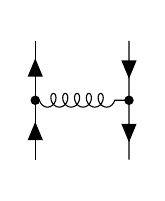
\begin{tikzpicture}[scale=0.7, transform shape, baseline={([yshift=-0.1cm]current bounding box.center)}]
    \begin{feynman}
    
    \vertex [dot] (a) {};
    \vertex [above=1.2cm of a] (v1) {};
    \vertex [below=1.2cm of a] (v2) {};
    \vertex [dot, right=1.7cm of a] (b) {};
    \vertex [above=1.2cm of b] (w1) {};
    \vertex [below=1.2cm of b] (w2) {};

    \diagram* {
      (v2) -- [fermion] (a) -- [fermion] (v1), (w1) -- [fermion] (b) -- [fermion] (w2),
      (a) -- [gluon] (b)
    };
    \end{feynman}
    \end{tikzpicture} 
    = \frac{1}{2}\bigg( 
    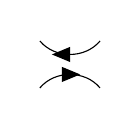
\begin{tikzpicture}[scale=0.7, transform shape, baseline={([yshift=-0.1cm]current bounding box.center)}]
    \begin{feynman}
    
    \vertex (a) {};
    \vertex [right=1.3cm of a] (a1) {};
    
    \vertex [below=1.1cm of a] (b) {};
    \vertex [below=1.1cm of a1] (b1) {};

    \diagram* {
      (a) -- [anti fermion, bend right=50] (a1), (b) -- [fermion, bend left=50] (b1)
    };
    \end{feynman}
    \end{tikzpicture}
    + 
    \begin{tikzpicture}[scale=0.7, transform shape, baseline={([yshift=-0.1cm]current bounding box.center)}]
    \begin{feynman}
    
    \vertex (a) {};
    \vertex [above=1.2cm of a] (a1) {};
    
    \vertex [right=0.5cm of a] (b) {};
    \vertex [above=1.2cm of b] (b1) {};

    \diagram* {
      (a) -- [fermion] (a1), (b) -- [anti fermion] (b1)
    };
    \end{feynman}
    \end{tikzpicture} \bigg),
\end{equation}
from which we can connect the lower quark index to make the self-energy colour factor
\begin{equation}
    \feynmandiagram[inline=(v.base), layered layout, horizontal=a to b, scale=0.7, transform shape] { 
            a -- [fermion] v [dot] -- [gluon, half left, looseness=1.5] v1 [dot], v -- v1, v1 -- [fermion] b }; = \frac{1}{2}\bigg( 
    \begin{tikzpicture}[scale=0.7, transform shape, baseline={([yshift=-0.1cm]current bounding box.center)}]
    \begin{feynman}
    
    \vertex (a) {};
    \vertex [right=1.1cm of a] (a1) {};
    \vertex [below=1.1cm of a] (b) {};
    \vertex [below=1.1cm of a1] (b1) {};
    \vertex [above=0.3cm of b] (c) {};
    \vertex [above=0.3cm of b1] (c1) {};

    \diagram* {
      (a) -- [fermion] (a1), (b) -- [anti fermion, half left] (b1), (c) -- [half right] (c1)
    };
    \end{feynman}
    \end{tikzpicture}
    -\frac{1}{n_c}\feynmandiagram[inline={([yshift=-0.1cm]current bounding box.center)}, horizontal=a to b, scale=0.7, transform shape] { a -- [fermion] b };
    \bigg) = C_F(\feynmandiagram[inline={([yshift=-0.1cm]current bounding box.center)}, horizontal=a to b, scale=0.7, transform shape] { a -- [fermion] b };),\quad \begin{tikzpicture}[scale=0.1, transform shape, baseline={([yshift=-0.1cm]current bounding box.center)}]
    \begin{feynman}
    
    \vertex (b) {};
    \vertex [right=1.1cm of a1] (b1) {};
    \vertex [above=0.3cm of b] (c) {};
    \vertex [above=0.3cm of b1] (c1) {};

    \diagram* {
        (b) -- [anti fermion, half left] (b1), (c) -- [half right] (c1)
    };
    \end{feynman}
    \end{tikzpicture} = n_c.
\end{equation}

\section{Tree-level amplitudes}
Having arranged the colour factors it is also worth noting how we can compute compact helicity amplitudes for the remaining kinematic components. We will introduce the concepts by means of the $\qbar qgg$ scattering. There are three tree-level Feynman diagrams that make up the total amplitude
\begin{equation}
    \amp = \begin{tikzpicture}[scale=0.7, transform shape, baseline={([yshift=-0.1cm]current bounding box.center)}]
    \begin{feynman}
    
    \vertex [dot] (a) {};
    \vertex [dot, above=1.7cm of a] (b) {};
    
    \vertex [right=1.2cm of a] (v1) {4};
    \vertex [left=1.2cm of a] (v2) {1};
    \vertex [right=1.2cm of b] (w1) {3};
    \vertex [left=1.2cm of b] (w2) {2};

    \diagram* {
      (a) -- [fermion] (b), (v2) -- [fermion] (a) -- [gluon] (v1), (w2) -- [anti fermion] (b) -- [gluon] (w1)
    };
    \end{feynman}
    \end{tikzpicture} + \begin{tikzpicture}[scale=0.7, transform shape, baseline={([yshift=-0.1cm]current bounding box.center)}]
    \begin{feynman}
    
    \vertex [dot] (a) {};
    \vertex [dot, above=1.7cm of a] (b) {};
    
    \vertex [right=1.2cm of a] (v1) {4};
    \vertex [left=1.2cm of a] (v2) {1};
    \vertex [right=1.2cm of b] (w1) {3};
    \vertex [left=1.2cm of b] (w2) {2};

    \diagram* {
      (a) -- [fermion] (b), (v2) -- [fermion] (a) -- [gluon] (w1), (w2) -- [anti fermion] (b) -- [gluon] (v1)
    };
    \end{feynman}
    \end{tikzpicture} +
    \begin{tikzpicture}[scale=0.7, transform shape, baseline={([yshift=-0.1cm]current bounding box.center)}]
    \begin{feynman}
    
    \vertex [dot] (a) {};
    \vertex [above left=1.2cm and 0.7 of a] (v1) {2};
    \vertex [below left=1.2cm and 0.7 of a] (v2) {1};
    \vertex [dot, right=1.7cm of a] (b) {};
    \vertex [above right=1.2cm and 0.7 of b] (w1) {3};
    \vertex [below right=1.2cm and 0.7 of b] (w2) {4};

    \diagram* {
      (v2) -- [fermion] (a) -- [fermion] (v1), (w1) -- [gluon] (b) -- [gluon] (w2),
      (a) -- [gluon] (b)
    };
    \end{feynman}
    \end{tikzpicture}
    ,
\end{equation}
where we have chosen all particles out-going to simply the momentum conservation to $\sum_{i=1}^4p_i^\mu = 0$. Firstly, let's show that the amplitude satisfies the Ward identity $\amp^\mu p_{3\mu} = 0$ where $\amp = \amp^\mu \epsilon_\mu(p_3)$. The first diagram reads
\begin{equation}
    \amp_1 = i(ig_S)^2\ubar_1\slep_4\frac{\slp_{23}}{s_{23}}\slep_3v_2(t^{a_3}t^{a_4})_{i_2i_4},
\end{equation}
where $p_{ij} = p_i + p_j$ and $s_{ij} = 2(p_i \cdot p_j)$. The contribution to the Ward identity is then
\begin{equation}
    \begin{split}
        \amp_1^\mu p_{3\mu} &= -ig_S^2\ubar_1\slep_4\frac{\slp_{23}}{s_{23}}\slp_3v_2c_1 \\
        &= -ig_S^2\ubar_1\slep_4\frac{\slp_2\slp_3}{s_{23}}v_2c_1 \\
        &= -ig_S^2\ubar_1\slep_4v_2c_1,
    \end{split}
\end{equation}
where $c_1 \equiv (t^{a_3}t^{a_4})_{i_2i_1}$ and in the last step we used the Clifford algebra. The second diagram is related to the first through a swap of indices $3 \leftrightarrow 4$, doing that results in the contribution
\begin{equation}
    \amp_2^\mu p_{3\mu} = ig_S^2\ubar_1\slep_4v_2c_2,\quad c_2 \equiv (t^{a_4}t^{a_3})_{i_2i_1}.
\end{equation}
The third diagram however is not so simple to derive, the amplitude is 
\begin{equation}
    \begin{split}
        \amp_3 &= g_S\ubar_1\gamma^\mu v_2\frac{1}{s_{12}}\hatV_{3g\mu\mu_3\mu_4}(-p_{34},p_3,p_4)\epsilon^{\mu_1}_3\epsilon^{\mu_4}_4 t^b_{i_1i_2}f^{ba_3a_4} \\
        &= g_S^2t^b_{i_1i_2}f^{ba_3a_4}\frac{1}{s_{12}}\ubar_1\gamma^\mu v_2 \\
        &\times[(\epsilon_3\cdot\epsilon_4)(p_3 - p_4)_\mu + \epsilon_{4\mu}(2p_4 \cdot \epsilon_3) - \epsilon_{3\mu}(2p_3 \cdot p_4)],
    \end{split}
\end{equation}
where we have made use of $\epsilon_i\cdot p_i = 0$. For the Ward identity the contribution of this third diagram is
\begin{equation}
    \begin{split}
        \amp_3^\mu p_{3\mu} &= g_S^2t^b_{i_1i_2}f^{ba_3a_4}\frac{1}{s_{12}}\ubar_1\gamma^\mu v_2\bigg[\epsilon_{4\mu}s_{12} - (p_3\cdot \epsilon_4)(p_3 + p_4)_\mu\bigg] \\
        &= g_S^2c_3\ubar_1\slep_4v_2,
    \end{split}
\end{equation}
where we identified $c_3 \equiv t^b_{i_1i_2}f^{ba_3a_4}$, which can be written as
\begin{equation}
    c_3 \equiv t^b_{i_1i_2}f^{ba_3a_4} = -i\comm{t^{a_3}}{t^{a_4}}_{i_1i_2} = -i(c_1 - c_2).
\end{equation}
This is now sufficient to show that $\amp$ satisfies the Ward identity as
\begin{equation}
    \amp^\mu p_{3\mu} = g_S^2\ubar_1\slep_4v_2(-ic_1 + ic_2 - c_3) = 0.
\end{equation}
The colour identity above can be used to order the diagrams that appear in the amplitude; defining
\begin{equation}
    \amp_1 := g_S^2c_1\amp_1,\quad \amp_2 := g_S^2c_2\amp_2,\quad \amp_3 := ig_S^2c_3\amp_3,
\end{equation}
we have
\begin{equation}
    \amp = g_S^2[c_1(\amp_1 + \amp_3) + c_2(\amp_1 - \amp_3)],
\end{equation}
where the partial amplitudes are related by symmetry 
\begin{equation}
    (\amp_1 + \amp_3)|_{3\leftrightarrow 4} = \amp_2 - \amp_3.
\end{equation}
It is therefore sufficient to compute only two of the three diagrams and then permute the result. This process is precisely the colour ordering. 

Compact representations for the helicity amplitudes can be found using the spinor-helicity formalism, built around the Weyl representation for the Dirac equation from which we construct everything from two-component helicity spinors, like
\begin{equation}
    \amp(1_q^{h_1}2^{h_2}_{\qbar}3^{h_3}_g4^{h_4}_g) = \amp_1 + \amp_3|_{\ubar_1 \to \frac{1}{2}(1 + h_1\gamma_5)u_2 ,\dots}.
\end{equation}
We recall the Weyl representation of the Dirac matrices 
\begin{equation}
    \gamma^\mu = 
    \begin{pmatrix}
        \MO & \sigma^\mu \\
        \bsigma^\mu & \MO
    \end{pmatrix},\quad \sigma^\mu = (\MI,\vsigma),\,\bsigma^\mu = (-\MI,\vsigma).
\end{equation}
The helicity projection operators are
\begin{equation}
    P_\pm = \frac{1}{2}(\MI \pm \gamma_5) = \frac{1}{2}
    \begin{pmatrix}
        \MI \pm \MI & \MO \\
        \MO & \MI \mp \MI
    \end{pmatrix},
\end{equation}
from which we form the helicty operators
\begin{equation}
    \begin{cases}
        u_+ = p_+u = 
        \begin{pmatrix}
            \ket{p} \\
            0
        \end{pmatrix} = v_- \\[3ex]
        u_- = p_-u = 
        \begin{pmatrix}
            0 \\
            \sqket{p}
        \end{pmatrix} = v_+
    \end{cases}.
\end{equation}
Explicit solutions for the two-component Weyl spinors $\ket{p}$ and $\sqket{p}$ can be found satisfying 
\begin{align}
    \begin{cases}
        \ket{p}\sqbra{p} = \sigma \cdot p \\
        \sqket{p}\bra{p} = \bsigma \cdot p
    \end{cases}\quad\longleftrightarrow\quad
    \begin{cases}
        p^\mu = \dfrac{1}{2}\sqketbra{p\sigma^\mu p} \\[2ex]
        p^\mu = \dfrac{1}{2}\sqbraket{p\sigma^\mu p}
    \end{cases},
\end{align}
where $\bra{p} = \epsilon\ket{p}$ and $\sqbra{p} = \epsilon\sqket{p}$.

\section{Divergent graphs at 1-loop}
The UV divergences are similar to those in QED, which are collected in table \ref{tab: UV divergences QCD}, where we have omitted the tadpole graph which is trivially zero because of the colour algebra. The last two graphs do not match gauge invariant operators and must therefore give finite results when all diagrams are summed together. The major difference with respect to QED is the number of diagrams that contribute. Up to 1-loop we have
\begin{equation}
    \feynmandiagram[inline={([yshift=-0.1cm]current bounding box.center)}, horizontal=a to c, scale=0.8, transform shape, layered layout] { 
         a -- [fermion] b [blob] -- [fermion] c }; = 
    \feynmandiagram[inline={([yshift=-0.1cm]current bounding box.center)}, horizontal=a to b, scale=0.8, transform shape, layered layout] { 
         a -- [fermion] b }; + 
    \feynmandiagram[inline={([yshift=-0.3cm]current bounding box.center)}, layered layout, horizontal=a to b, scale=0.8, transform shape] { 
        a -- [fermion] v -- [gluon, half left, looseness=1.5] v1, v -- v1, v1 -- [fermion] b };,
\end{equation}
\begin{equation}
\begin{aligned}
    \feynmandiagram[inline={([yshift=-0.1cm]current bounding box.center)}, horizontal=a to c, scale=0.8, transform shape, layered layout] { 
         a -- [gluon] b [blob] -- [gluon] c, 
         }; &= 
    \feynmandiagram[inline={([yshift=-0.1cm]current bounding box.center)}, horizontal=a to b, scale=0.8, transform shape, layered layout] { 
         a -- [gluon] b, 
         }; +
    \feynmandiagram[inline={([yshift=-0.1cm]current bounding box.center)}, layered layout, horizontal=a to b, scale=0.8, transform shape] { 
        a -- [gluon] v [dot] -- [gluon, half left, looseness=1.5] v1 [dot], v1 -- [gluon, half left, looseness=1.5] v, v1 -- [gluon] b , 
        }; + \nsum_q
    \feynmandiagram[inline={([yshift=-0.1cm]current bounding box.center)}, layered layout, horizontal=a to b, scale=0.8, transform shape] { 
        a -- [gluon] v [dot] -- [fermion, half left, looseness=1.5] v1 [dot], v1 -- [fermion, half left, looseness=1.5] v, v1 -- [gluon] b , 
        }; \\
        &+ \feynmandiagram[inline={([yshift=-0.1cm]current bounding box.center)}, layered layout, horizontal=a to b, scale=0.7, transform shape] { 
        a -- [gluon] v [dot] -- [ghost, half left, looseness=1.5] v1 [dot], v1 -- [ghost, half left, looseness=1.5] v, v1 -- [gluon] b , 
        };,
\end{aligned}
\end{equation}
\begin{equation}
    \feynmandiagram[inline={([yshift=-0.1cm]current bounding box.center)}, horizontal=a to c, scale=0.8, transform shape, layered layout] { 
         a -- [ghost] b [blob] -- [ghost] c }; =
    \feynmandiagram[inline={([yshift=-0.1cm]current bounding box.center)}, horizontal=a to b, scale=0.8, transform shape, layered layout] { 
         a -- [ghost] b }; + 
    \feynmandiagram[inline={([yshift=-0.3cm]current bounding box.center)}, layered layout, horizontal=a to b, scale=0.8, transform shape] { 
        a -- [ghost] v [dot] -- [gluon, half left, looseness=1.5] v1 [dot], v -- [ghost] v1, v1 -- [ghost] b };,
\end{equation}
\begin{equation}
\begin{aligned}
    \feynmandiagram[inline={([yshift=-0.1cm]current bounding box.center)}, horizontal=a to c, scale=0.8, transform shape, node distance=1.2cm] { 
        a -- [fermion] b [blob, minimum size=0.3 cm, inner sep=0pt] -- [fermion] c, b -- [gluon] d, }; &= 
    \feynmandiagram[inline={([yshift=-0.1cm]current bounding box.center)}, horizontal=a to c, scale=0.8, transform shape, node distance=1.2cm] { 
        a -- [fermion] b [dot] -- [fermion] c, b -- [gluon] d, }; +
    \feynmandiagram[inline={([yshift=-0.1cm]current bounding box.center)}, horizontal=v1 to v2, scale=0.8, transform shape, node distance=0.8cm]{
        a -- [fermion] v1,
        b -- [fermion] v2,
        c -- [gluon] v3,
    
        v1 -- [gluon] v2
           -- [fermion] v3
           -- [fermion] v1 }; +
    \feynmandiagram[inline={([yshift=-0.1cm]current bounding box.center)}, horizontal=v1 to v2, scale=0.8, transform shape, node distance=0.8cm]{
        a -- [fermion] v1,
        b -- [fermion] v2,
        c -- [gluon] v3 [dot],
    
        v1 -- [fermion] v2
           -- [gluon] v3
           -- [gluon] v1 }; \\
    &+ \feynmandiagram[inline={([yshift=-0.1cm]current bounding box.center)}, horizontal=v to v1, scale=0.8, transform shape] { 
        a [label=\ensuremath{1}] -- [gluon] v [dot] -- [gluon, half left, looseness=1.5] v1 [dot], a1 [label=\ensuremath{2}] -- [gluon] v, v1 -- [gluon, half left, looseness=1.5] v, v1 -- [gluon] b [label=\ensuremath{3}], 
        }; +
    \feynmandiagram[inline={([yshift=-0.1cm]current bounding box.center)}, horizontal=v to v1, scale=0.8, transform shape] { 
        a [label=\ensuremath{1}] -- [gluon] v [dot] -- [gluon, half left, looseness=1.5] v1 [dot], a1 [label=\ensuremath{3}] -- [gluon] v, v1 -- [gluon, half left, looseness=1.5] v, v1 -- [gluon] b [label=\ensuremath{2}], 
        };  +
    \feynmandiagram[inline={([yshift=-0.1cm]current bounding box.center)}, horizontal=v to v1, scale=0.8, transform shape] { 
        a [label=\ensuremath{2}] -- [gluon] v [dot] -- [gluon, half left, looseness=1.5] v1 [dot], a1 [label=\ensuremath{3}] -- [gluon] v, v1 -- [gluon, half left, looseness=1.5] v, v1 -- [gluon] b [label=\ensuremath{1}], 
        };, \\
    &+ \mathrm{ghost\,loops} + \mathrm{quark\,loops},
\end{aligned}
\end{equation}
\begin{equation}
    \feynmandiagram[inline={([yshift=-0.1cm]current bounding box.center)}, horizontal=a to c, scale=0.8, transform shape, node distance=1.2cm] { 
        a -- [ghost] b [blob, minimum size=0.3 cm, inner sep=0pt] -- [ghost] c, b -- [gluon] d }; = 
    \feynmandiagram[inline={([yshift=-0.1cm]current bounding box.center)}, horizontal=a to c, scale=0.8, transform shape, node distance=1.2cm] { 
        a -- [ghost] b [dot] -- [ghost] c, b -- [gluon] d }; +
    \feynmandiagram[inline={([yshift=-0.1cm]current bounding box.center)}, horizontal=v1 to v2, scale=0.8, transform shape, node distance=0.8cm]{
        a -- [ghost] v1 [dot],
        b -- [ghost] v2 [dot],
        c -- [gluon] v3 [dot],
    
        v1 -- [gluon] v2
           -- [ghost] v3
           -- [ghost] v1 }; +
    \feynmandiagram[inline={([yshift=-0.1cm]current bounding box.center)}, horizontal=v1 to v2, scale=0.8, transform shape, node distance=0.8cm]{
        a -- [ghost] v1 [dot],
        b -- [ghost] v2 [dot],
        c -- [gluon] v3 [dot],
    
        v1 -- [ghost] v2
           -- [gluon] v3
           -- [gluon] v1 };.
\end{equation}
If required, 4-points diagram expansions can be obtained relatively easily, clearly there are quite a few diagrams to consider. 
\begin{table}[h]
    \centering
    \begin{tabular}{|c|ccccc|}
         \hline 
         $\Gamma$ & $n_q$ & $n_g$ & $n_c$ & $\omega(\Gamma)$ & name \\ \hline
         \feynmandiagram[inline={([yshift=0cm]current bounding box.center)}, horizontal=a to c, scale=0.8, transform shape, layered layout] { 
         a -- [fermion] b [blob] -- [fermion] c, 
         }; & 2 & 0 & 0 & 1 & quark self-energy \\
         \feynmandiagram[inline={([yshift=0cm]current bounding box.center)}, horizontal=a to c, scale=0.8, transform shape, layered layout] { 
         a -- [gluon] b [blob] -- [gluon] c, 
         }; & 0 & 2 & 0 & 2 & gluon self-energy\\ 
         \feynmandiagram[inline={([yshift=0cm]current bounding box.center)}, horizontal=a to c, scale=0.7, transform shape, node distance=1.2cm] { 
         a -- [fermion] b [blob, minimum size=0.3 cm, inner sep=0pt] -- [fermion] c, b --  [gluon] d, 
         }; & 2 & 1 & 0 & 0 & $q\qbar g$ vertex\\ 
         \feynmandiagram[inline={([yshift=0cm]current bounding box.center)}, horizontal=a to c, scale=0.7, transform shape, node distance=1.2cm] { 
         a -- [gluon] b [blob, minimum size=0.3 cm, inner sep=0pt] -- [gluon] c, b -- [gluon] d, 
         }; & 0 & 3 & 0 & 1 & 3$g$ vertex \\ 
         \feynmandiagram[inline={([yshift=0cm]current bounding box.center)}, horizontal=a to c, scale=0.7, transform shape, node distance=0.9cm] { 
         a -- [gluon] b [blob, minimum size=0.3 cm, inner sep=0pt] -- [gluon] c, b -- [gluon] d, b -- [gluon] e , 
         }; & 0 & 4 & 0 & 0 & 4$g$ vertex \\ 
         \feynmandiagram[inline={([yshift=-0.1cm]current bounding box.center)}, horizontal=a to c, scale=0.8, transform shape, layered layout] { 
         a -- [ghost] b [blob] -- [ghost] c, 
         }; & 0 & 0 & 2 & 2 & ghost self-energy\\ 
         \feynmandiagram[inline={([yshift=-0.1cm]current bounding box.center)}, horizontal=a to c, scale=0.7, transform shape, node distance=1.2cm] { 
         a -- [ghost] b [blob, minimum size=0.3 cm, inner sep=0pt] -- [ghost] c, b -- [gluon] d, 
         }; & 0 & 1 & 2 & 1 & $c\cbar g$ vertex \\ 
         \feynmandiagram[inline={([yshift=-0.1cm]current bounding box.center)}, horizontal=a to c, scale=0.7, transform shape, node distance=0.9cm] { 
         a -- [ghost] b [blob, minimum size=0.3 cm, inner sep=0pt] -- [ghost] c, b --  [gluon] d, b -- [gluon] e , 
         }; & 0 & 2 & 2 & 0 & - \\ 
         \feynmandiagram[inline={([yshift=-0.1cm]current bounding box.center)}, horizontal=a to c, scale=0.7, transform shape, node distance=0.8cm] { 
         a -- [ghost] b [blob, minimum size=0.3 cm, inner sep=0pt] -- [ghost] c, b -- [ghost] d, b -- [ghost] e , 
         }; & 0 & 0 & 4 & 0 & - \\ \hline 
    \end{tabular}
    \caption{UV divergences in QCD.}
    \label{tab: UV divergences QCD}
\end{table}

\subsection{Renormalization counter-terms}
The necessary field and parameter redefinitions are as follows
\begin{gather}
    \psi_{0q} = Z_{\psi_q}^{1/2}\psi_{q,R},\quad A^\mu_0 = Z_A^{1/2}A_R^\mu,\quad c_0 = Z_c^{1/2}c_R, \\
    m_{0q} = Z_{m_q}m_{q,R},\quad g_{S,0} = g_{S,R}\mu_R^\epsilon Z_{g_S}.
\end{gather}
\begin{notz}
    For the rest of the discussion, quantities without the $R$ subscript will be considered to be renormalized. 
\end{notz}
The QCD Lagrangian in terms of renormalized quantities has the following counter-terms
\begin{equation}
    \begin{split}
        \dL_{QCD} &= \dL_{QCD,R} + \sum_{q=1}^{n_f}[i\psib_q\slpd\psi_q(Z_{\psi_q} - 1) + m_q\psib_q\psi_q(Z_{m_q}Z_{\psi_q} -1) \\
        &-g_S\mu_R^\epsilon\psib_q\slA^at^a\psi_q(Z_1 - 1) - \cbar^a\square c^a(Z_c - 1)] \\
        &- g_s\mu_R^\epsilon f^{abc}\p_\mu\cbar^a A^{\mu b}c^c(Z_1^c - 1) \\
        &+\frac{1}{2}A^a_\mu(g^{\mu\nu}\square - \p^\mu\p^\nu)A_\nu^a(Z_A -1 ) \\
        &+g_S\mu_R^\epsilon f^{abc}A^{\mu b}A^{\nu c}\p_\mu A_\nu^a(Z_1^{3g} - 1) \\
        &-\frac{1}{4}g_S^2\mu_R^{2\epsilon}f^{abx}f^{xcd}A_\mu^a A_\nu^b A^{\mu c}A^{\nu d}(Z_1^{4g} -1),
    \end{split}
\end{equation}
where
\begin{gather}
    Z_1 = Z_{g_S}Z_A^{1/2}Z_{\psi_q},\quad Z_1^c = Z_{g_S}Z_A^{1/2}Z_c, \\
    Z_1^{3g} = Z_{g_S}Z_A^{3/2},\quad Z_1^{4g} = Z_{g_S}^2Z_A^2.
\end{gather}
Unlike QED the gauge invariance constraints on $Z_x$ do not imply that $Z_1 = Z_{\psi_q}$. There are a set of relations for correlation functions that follows from gauge invariance called ``Slavrov-Taylor identities'', in turn we may derive additional constraints on $Z_x$ but we can not avoid the vertex amputation. 
\begin{center}
    \begin{tikzpicture}[
        box/.style={rectangle,draw,rounded corners=2mm,thin, minimum width=2.5cm, minimum height=1.4cm, align=center}, node distance=1.2cm
        ]
        
        \node[box] (a) {$U(1)$ gauge invariance};
        \node[above=0.2cm of a, font=\bfseries\Large] {\underline{QED}};
        \node[box, below left=of a] (b) {$Z_1 = Z_\psi$};
        \node[box, below right=of a, minimum width=2.5cm] (c) {Ward-Takahashi \\ identity};
        
        \draw[->] (a) -- (b);
        \draw[->] (a) -- (c);
        \draw[<-] (b) -- (c);
    \end{tikzpicture}
\end{center}
\begin{center}
    \begin{tikzpicture}[
        box/.style={rectangle,draw,rounded corners=2mm,thin, minimum width=2.5cm, minimum height=1.4cm, align=center}, node distance=1.2cm
        ]
        
        \node[box] (a) {$SU(n_c)$ gauge invariance};
        \node[above=0.2cm of a, font=\bfseries\Large] {\underline{QCD}};
        \node[box, below left=of a] (b) {$\dfrac{Z_1}{Z_{\psi_q}} = \dfrac{Z_1^c}{Z_c},\dots$};
        \node[box, below right=of a, minimum width=2.5cm] (c) {Slavrov-Taylor \\ identities};
        
        \draw[->] (a) -- (b);
        \draw[->] (a) -- (c);
        \draw[<-] (b) -- (c);
    \end{tikzpicture}
\end{center}
If we were to write down all $SU(n_c)$ gauge invariant operators in four dimensions we would include 
\begin{equation}
    F^{\mu\nu a}\tilde{F}^a_{\mu\nu},\quad \tilde{F}^a_{\mu\nu} \equiv \epsilon_{\mu\nu\rho\sigma}F^{\rho\sigma a}.
\end{equation}
This term represents a subtle problem in QCD in which its presence implies CP violating strong interactions which are not observed experimentally. It is possible to show that 
\begin{equation}
    F^{\mu\nu a}\tilde{F}^a_{\mu\nu} = \p_\mu k^\mu,
\end{equation}
where
\begin{equation}
    k^\mu = \epsilon^{\mu\nu\rho\sigma}A_\nu^a(F^a_{\rho\sigma} - \frac{g_S}{3}f^{abc}A_\rho^bA^c_\sigma).
\end{equation}
As a result, we see the operator $F^{\mu\nu a}\tilde{F}^a_{\mu\nu}$ can be written as a total derivative and plays no role in perturbation theory. QED, an Abelian theory, could also have a term $F^{\mu\nu a}\tilde{F}^a_{\mu\nu}$ but this total derivative has no non-perturbative consequences. 't Hooft showed that the QCD, a non-Abelian theory, vacuum has instanton contributions so $F^{\mu\nu a}\tilde{F}^a_{\mu\nu}$ also have non-perturbative consequences. A proposed solution to this problem introduces a new dynamical field, the ``axion'', which can naturally tune the coefficient at $F^{\mu\nu a}\tilde{F}^a_{\mu\nu}$ to be very small, namely undetectable. This is the Peccei-Quinn mechanism. Nonetheless, so far axions have not been confirmed in experiments.

\subsection{1-loop graph computations}
\paragraph{Quark self-energy.} There is only one diagram and the only difference with respect to QED is the colour factor, so
\begin{equation}
    \begin{aligned}
        \feynmandiagram[inline={([yshift=-0.2cm]current bounding box.center)}, layered layout, horizontal=a to b, scale=0.7, transform shape] { 
        a [label=\ensuremath{i}] -- [fermion] v -- [gluon, half left, looseness=1.5, momentum={[arrow distance=6pt]\ensuremath{\scriptstyle k}}] v1, v -- [momentum'={[arrow distance = 4pt]\ensuremath{\scriptstyle -k+p}}] v1, v1 -- [fermion] b [label=\ensuremath{j}], 
        }; &= t^a_{ik}t^a_{kj}g_S^2\mu_R^{2\epsilon}\int\frac{d^Dx}{(2\pi)^D}\frac{\gamma^\mu(-\slk + \slp + m_q)\gamma_\mu}{D(k,0)D(k-p,m)_q} \\
        &= C_F\delta_{ij}\frac{i\alpha_Sr_\Gamma}{4\pi}\bigg[\frac{1}{\epsilon}(\slp - 4m_q) + o(\epsilon^0)\bigg],
    \end{aligned}
\end{equation}
as for the counter-term we have
\begin{equation}
    \feynmandiagram[inline={([yshift=-0.1cm]current bounding box.center)}, horizontal=a to c, scale=0.8, transform shape, layered layout] { a -- [fermion] b [crossed dot] -- [fermion] c }; = i\delta_{ij}(\delta_{\psi_q}\slp - \delta_3m_q) = i\delta_{ij}[\delta_{\psi_q}(\slp - m_q) - \delta_{m_q}m_q].
\end{equation}
Since for the strong interaction there is no perturbative low energy limit we cannot perform an on-shell renormalization and so stick to $\MMS$
\begin{equation}
    \delta^{(1)}_{\psi_q} = \frac{\alpha_Sr_\Gamma}{4\pi}\bigg(-\frac{1}{\epsilon}\bigg),\quad \delta^{(1)}_{m_q} = \frac{\alpha_Sr_\Gamma}{4\pi}\bigg(-\frac{3}{\epsilon}\bigg).
\end{equation}

\paragraph{Gluon self-energy.} The QCD computation differs from the QED analogue in that there are more diagrams and the ghost diagrams are required to produce the correct transverse tensor structure dictated by gauge invariance. 
\begin{equation}
    \feynmandiagram[inline={([yshift=-0.1cm]current bounding box.center)}, layered layout, horizontal=a to b, scale=0.8, transform shape] { 
        a -- [gluon] v [dot] -- [gluon, half left, looseness=1.5] v1 [dot], v1 -- [gluon, half left, looseness=1.5] v, v1 -- [gluon] b }; + \nsum_q
    \feynmandiagram[inline={([yshift=-0.1cm]current bounding box.center)}, layered layout, horizontal=a to b, scale=0.8, transform shape] { 
        a -- [gluon] v [dot] -- [fermion, half left, looseness=1.5] v1 [dot], v1 -- [fermion, half left, looseness=1.5] v, v1 -- [gluon] b }; + 
    \feynmandiagram[inline={([yshift=-0.1cm]current bounding box.center)}, layered layout, horizontal=a to b, scale=0.7, transform shape] { 
        a -- [gluon] v [dot] -- [ghost, half left, looseness=1.5] v1 [dot], v1 -- [ghost, half left, looseness=1.5] v, v1 -- [gluon] b }; +
    \underbrace{\feynmandiagram[inline={([yshift=-0.5cm]current bounding box.center)}, horizontal=a to c, scale=0.7, transform shape, layered layout]{
        a -- [fermion] b [dot]-- [fermion] c,
        b -- [gluon, out=60, in=120, loop, min distance=1.5cm] b,
    };}_{\substack{zero\,in\\dim.\,reg.}}
\end{equation}
Let's start with the colour part of the gluon diagram
\begin{equation}
    \feynmandiagram[inline={([yshift=-0.1cm]current bounding box.center)}, layered layout, horizontal=a to b, scale=0.8, transform shape] { 
        a -- [gluon, edge label=\ensuremath{a}, pos=0.1] v [dot] -- [gluon, half left, looseness=1.5, edge label=\ensuremath{x}, pos=0.1] v1 [dot], v1 -- [gluon, half left, looseness=1.5, edge label=\ensuremath{y}, pos=0.1] v, v1 -- [gluon, edge label=\ensuremath{b}, pos=0.9] b }; = f^{axy}f^{byx}.
\end{equation}
We may already anticipate that this should be proportional to the tree-level colour factor $\delta^{ab}$, namely
\begin{equation}
    \feynmandiagram[inline={([yshift=-0.1cm]current bounding box.center)}, layered layout, horizontal=a to b, scale=1, transform shape] { a -- [gluon] v [dot] -- [gluon, half left, looseness=1.5] v1 [dot], v1 -- [gluon, half left, looseness=1.5] v, v1 -- [gluon] b }; \propto \feynmandiagram[inline={([yshift=-0.1cm]current bounding box.center)}, horizontal=a to b, scale=1, transform shape, layered layout] { a -- [gluon] b };.
\end{equation}
By writing $f^{abc} = -2i\tr{\comm{t^a}{t^b}t^c}$ and applying the Fierz identity, we can derive the constant of proportionality
\begin{equation}
    \begin{aligned}
        \feynmandiagram[inline={([yshift=-0.1cm]current bounding box.center)}, layered layout, horizontal=a to b, scale=0.8, transform shape] { 
        a -- [gluon, edge label=\ensuremath{a}, pos=0.1] v [dot] -- [gluon, half left, looseness=1.5] v1 [dot], v1 -- [gluon, half left, looseness=1.5] v, v1 -- [gluon, edge label=\ensuremath{b}, pos=0.9] b };
        &= 4(
        \begin{tikzpicture}[scale=0.7, transform shape, baseline={([yshift=-0.1cm]current bounding box.center)}]
        \begin{feynman}
        
        \vertex [label=\ensuremath{a}](a) {};
        \vertex [right=1cm of a, draw, circle, minimum size=0.6cm, inner sep=0pt] (v) {};
        \vertex [label=\ensuremath{x}, above right=0.5cm and 1cm of v] (b) {};
        \vertex [label=\ensuremath{y}, below right=0.5cm and 1cm of v] (c) {};
        
        \diagram* {
            (a) -- [gluon] (v),
            (v) -- [gluon] (b),
            (v) -- [gluon] (c),
        };
        
        \end{feynman}
        
        % freccia sulla circonferenza
        \draw[
            postaction={
                decorate,
                decoration={
                    markings,
                    mark=at position 0.2 with {\arrow{>}}
                }
            }
        ] (v.140) arc (140:-140:0.3cm);
    
    \end{tikzpicture} -
    \begin{tikzpicture}[scale=0.7, transform shape, baseline={([yshift=-0.1cm]current bounding box.center)}]
        \begin{feynman}
        
        \vertex [label=\ensuremath{a}](a) {};
        \vertex [right=1cm of a, draw, circle, minimum size=0.6cm, inner sep=0pt] (v) {};
        \vertex [label=\ensuremath{y}, above right=0.5cm and 1cm of v] (b) {};
        \vertex [label=\ensuremath{x}, below right=0.5cm and 1cm of v] (c) {};
        
        \diagram* {
            (a) -- [gluon] (v),
            (v) -- [gluon] (b),
            (v) -- [gluon] (c),
        };
        
        \end{feynman}
        
        % freccia sulla circonferenza
        \draw[
            postaction={
                decorate,
                decoration={
                    markings,
                    mark=at position 0.2 with {\arrow{>}}
                }
            }
        ] (v.140) arc (140:-140:0.3cm);
    
    \end{tikzpicture}) (
        \begin{tikzpicture}[scale=0.7, transform shape, baseline={([yshift=-0.1cm]current bounding box.center)}]
        \begin{feynman}
        
        \vertex [label=\ensuremath{a}](b) {};
        \vertex [right=1cm of a, draw, circle, minimum size=0.6cm, inner sep=0pt] (v) {};
        \vertex [label=\ensuremath{x}, above right=0.5cm and 1cm of v] (b) {};
        \vertex [label=\ensuremath{y}, below right=0.5cm and 1cm of v] (c) {};
        
        \diagram* {
            (a) -- [gluon] (v),
            (v) -- [gluon] (b),
            (v) -- [gluon] (c),
        };
        
        \end{feynman}
        
        % freccia sulla circonferenza
        \draw[
            postaction={
                decorate,
                decoration={
                    markings,
                    mark=at position 0.2 with {\arrow{>}}
                }
            }
        ] (v.140) arc (140:-140:0.3cm);
    
    \end{tikzpicture} -
    \begin{tikzpicture}[scale=0.7, transform shape, baseline={([yshift=-0.1cm]current bounding box.center)}]
        \begin{feynman}
        
        \vertex [label=\ensuremath{b}](a) {};
        \vertex [right=1cm of a, draw, circle, minimum size=0.6cm, inner sep=0pt] (v) {};
        \vertex [label=\ensuremath{y}, above right=0.5cm and 1cm of v] (b) {};
        \vertex [label=\ensuremath{x}, below right=0.5cm and 1cm of v] (c) {};
        
        \diagram* {
            (a) -- [gluon] (v),
            (v) -- [gluon] (b),
            (v) -- [gluon] (c),
        };
        
        \end{feynman}
        
        % freccia sulla circonferenza
        \draw[
            postaction={
                decorate,
                decoration={
                    markings,
                    mark=at position 0.2 with {\arrow{>}}
                }
            }
        ] (v.140) arc (140:-140:0.3cm);
    
    \end{tikzpicture}) \\
    &= 8(\begin{tikzpicture}[scale=0.8, transform shape, baseline={([yshift=-0.1cm]current bounding box.center)}]
    \begin{feynman}
    
    \vertex (a) {};
    \vertex [right=1cm of a, draw, circle, minimum size=0.6cm, inner sep=0pt] (v) {};
    \vertex [dot, above right=0.3cm and 0.1cm of v] (b) {};
    \vertex [dot, below right=0.3cm and 0.1cm of v] (c) {};
    \vertex [right=1.5cm of v, draw, circle, minimum size=0.6cm, inner sep=0pt] (v1) {};
    \vertex [dot, above left=0.3cm and 0.1cm of v1] (b1) {};
    \vertex [dot, below left=0.3cm and 0.1cm of v1] (c1) {};
    \vertex [right=1cm of v1] (d) {};
    
    \diagram* {
        (a) -- [gluon] (v),
        (b) -- [gluon, edge label=\ensuremath{x}, pos=0.1] (b1),
        (c) -- [gluon, edge label'=\ensuremath{y}, pos=0.1] (c1),
        (v1) -- [gluon] (d)
    };
    
    \end{feynman}
    
    % freccia sulla circonferenza
    \draw[
        postaction={
            decorate,
            decoration={
                markings,
                mark=at position 0.2 with {\arrow{>}}
            }
        }
    ] (v.170) arc (170:-170:0.3cm);

    \draw[
        postaction={
            decorate,
            decoration={
                markings,
                mark=at position 0.2 with {\arrow{>}}
            }
        }
    ] (v1.80) arc (80:-80:0.3cm);
    
    \end{tikzpicture} -
    \begin{tikzpicture}[scale=0.8, transform shape, baseline={([yshift=-0.1cm]current bounding box.center)}]
    \begin{feynman}
    
    \vertex (a) {};
    \vertex [right=1cm of a, draw, circle, minimum size=0.6cm, inner sep=0pt] (v) {};
    \vertex [dot, above right=0.3cm and 0.1cm of v] (b) {};
    \vertex [dot, below right=0.3cm and 0.1cm of v] (c) {};
    \vertex [right=1.5cm of v, draw, circle, minimum size=0.6cm, inner sep=0pt] (v1) {};
    \vertex [dot, above left=0.3cm and 0.1cm of v1] (b1) {};
    \vertex [dot, below left=0.3cm and 0.1cm of v1] (c1) {};
    \vertex [right=1cm of v1] (d) {};
    
    \diagram* {
        (a) -- [gluon] (v),
        (b) -- [gluon, edge label=\ensuremath{x}, pos=0.1] (c1),
        (c) -- [gluon, edge label'=\ensuremath{y}, pos=0.1] (b1),
        (v1) -- [gluon] (d)
    };
    
    \end{feynman}
    
    % freccia sulla circonferenza
    \draw[
        postaction={
            decorate,
            decoration={
                markings,
                mark=at position 0.2 with {\arrow{>}}
            }
        }
    ] (v.170) arc (170:-170:0.3cm);

    \draw[
        postaction={
            decorate,
            decoration={
                markings,
                mark=at position 0.2 with {\arrow{>}}
            }
        }
    ] (v1.80) arc (80:-80:0.3cm);
    
    \end{tikzpicture}).
    \end{aligned}
\end{equation}
The first term is 
\begin{equation}
    \begin{aligned}
        \begin{tikzpicture}[scale=0.8, transform shape, baseline={([yshift=-0.1cm]current bounding box.center)}]
        \begin{feynman}
        
        \vertex (a) {};
        \vertex [right=1cm of a, draw, circle, minimum size=0.6cm, inner sep=0pt] (v) {};
        \vertex [dot, above right=0.3cm and 0.1cm of v] (b) {};
        \vertex [dot, below right=0.3cm and 0.1cm of v] (c) {};
        \vertex [right=1.5cm of v, draw, circle, minimum size=0.6cm, inner sep=0pt] (v1) {};
        \vertex [dot, above left=0.3cm and 0.1cm of v1] (b1) {};
        \vertex [dot, below left=0.3cm and 0.1cm of v1] (c1) {};
        \vertex [right=1cm of v1] (d) {};
        
        \diagram* {
            (a) -- [gluon] (v),
            (b) -- [gluon, edge label=\ensuremath{x}, pos=0.1] (b1),
            (c) -- [gluon, edge label'=\ensuremath{y}, pos=0.1] (c1),
            (v1) -- [gluon] (d)
        };
        
        \end{feynman}
        
        % freccia sulla circonferenza
        \draw[
            postaction={
                decorate,
                decoration={
                    markings,
                    mark=at position 0.2 with {\arrow{>}}
                }
            }
        ] (v.170) arc (170:-170:0.3cm);
    
        \draw[
            postaction={
                decorate,
                decoration={
                    markings,
                    mark=at position 0.2 with {\arrow{>}}
                }
            }
        ] (v1.80) arc (80:-80:0.3cm);
        
        \end{tikzpicture} &= \frac{1}{2}(\begin{tikzpicture}[scale=0.8, transform shape, baseline={([yshift=-0.1cm]current bounding box.center)}]
    \begin{feynman}
    
    \vertex (a) {};
    \vertex [right=1.2cm of a, draw, circle, minimum size=0.8cm, inner sep=0pt] (v) {};
    \vertex [dot, below left=0.35cm and 0.3cm of v] (b) {};
    \vertex [dot, below right=0.35cm and 0.3cm of v] (c) {};
    \vertex [right=1.2cm of v] (d) {};
    
    
    \diagram* {
        (a) -- [gluon] (v),
        (b) -- [gluon, half right] (c), 
        (v) -- [gluon] (d)
    };
    
    \end{feynman}
    
    % freccia sulla circonferenza
    \draw[
        postaction={
            decorate,
            decoration={
                markings,
                mark=at position 0.2 with {\arrow{>}}
            }
        }
    ] (v.170) arc (170:-170:0.4cm);
    
    \end{tikzpicture} - \feynmandiagram[inline={([yshift=-0.1cm]current bounding box.center)}, layered layout, horizontal=a to b, scale=0.5, transform shape] { 
        a -- [gluon] v -- [fermion, half left, looseness=1.5] v1, v1 -- [fermion, half left, looseness=1.5] v, v1 -- [gluon] v2, v2 -- [fermion, half left, looseness=1.5] v3, v3 -- [fermion, half left, looseness=1.5] v2, v3 -- [gluon] b
        }; ) \\
        &=\frac{1}{4}\bigg(C_F - \frac{1}{2N_c}\bigg)(\feynmandiagram[inline={([yshift=-0.1cm]current bounding box.center)}, horizontal=a to b, scale=0.8, transform shape, layered layout] { a -- [gluon] b };),
    \end{aligned}
\end{equation}
where $\feynmandiagram[inline={([yshift=-0.1cm]current bounding box.center)}, layered layout, horizontal=a to b, scale=0.5, transform shape] { a -- [gluon, edge label=\ensuremath{a}, pos=0.1] v -- [fermion, half left, looseness=1.5] v1, v1 -- [fermion, half left, looseness=1.5] v, v1 -- [gluon, edge label=\ensuremath{b}, pos=0.9] b };   = \tr{t^at^b} = \delta^{ab}/2$, while the second term is
\begin{equation}
    \begin{aligned}
    \begin{tikzpicture}[scale=0.8, transform shape, baseline={([yshift=-0.1cm]current bounding box.center)}]
    \begin{feynman}
    
    \vertex (a) {};
    \vertex [right=1cm of a, draw, circle, minimum size=0.6cm, inner sep=0pt] (v) {};
    \vertex [dot, above right=0.3cm and 0.1cm of v] (b) {};
    \vertex [dot, below right=0.3cm and 0.1cm of v] (c) {};
    \vertex [right=1.5cm of v, draw, circle, minimum size=0.6cm, inner sep=0pt] (v1) {};
    \vertex [dot, above left=0.3cm and 0.1cm of v1] (b1) {};
    \vertex [dot, below left=0.3cm and 0.1cm of v1] (c1) {};
    \vertex [right=1cm of v1] (d) {};
    
    \diagram* {
        (a) -- [gluon] (v),
        (b) -- [gluon, edge label=\ensuremath{x}, pos=0.1] (c1),
        (c) -- [gluon, edge label'=\ensuremath{y}, pos=0.1] (b1),
        (v1) -- [gluon] (d)
    };
    
    \end{feynman}
    
    % freccia sulla circonferenza
    \draw[
        postaction={
            decorate,
            decoration={
                markings,
                mark=at position 0.2 with {\arrow{>}}
            }
        }
    ] (v.170) arc (170:-170:0.3cm);

    \draw[
        postaction={
            decorate,
            decoration={
                markings,
                mark=at position 0.2 with {\arrow{>}}
            }
        }
    ] (v1.80) arc (80:-80:0.3cm);
    
    \end{tikzpicture} &= \bigg(\begin{tikzpicture}[scale=0.7, transform shape, baseline={([yshift=-0.1cm]current bounding box.center)}]
    \begin{feynman}
    
    \vertex (a) {};
    \vertex [right=1.2cm of a, draw, circle, minimum size=1cm, inner sep=0pt] (v) {};
    \vertex [dot, below=0.5cm of v] (b) {};
    \vertex [dot, above=0.5cm of v] (c) {};
    \vertex [right=1.2cm of v] (d) {};
    
    
    \diagram* {
        (a) -- [gluon] (v),
        (b) -- [gluon] (c), 
        (v) -- [gluon] (d)
    };
    
    \end{feynman}
    
    % freccia sulla circonferenza
    \draw[
        postaction={
            decorate,
            decoration={
                markings,
                mark=at position 0.2 with {\arrow{>}}
            }
        }
    ] (v.190) arc (190:-190:0.5cm);
    
    \end{tikzpicture} - \frac{1}{N_c}\begin{tikzpicture}[scale=0.7, transform shape, baseline={([yshift=-0.1cm]current bounding box.center)}]
    \begin{feynman}
    
    \vertex (a) {};
    \vertex [right=1cm of a, draw, circle, minimum size=0.6cm, inner sep=0pt] (v) {};
    \vertex [right=0.15cm of v] (b) {};
    \vertex [right=1.5cm of v, draw, circle, minimum size=0.6cm, inner sep=0pt] (v1) {};
    \vertex [left=0.15cm of v1] (b1) {};
    \vertex [right=1cm of v1] (d) {};
    
    
    \diagram* {
        (a) -- [gluon] (v),
        (b) -- [gluon] (b1),
        (v1) -- [gluon] (d)
    };
    
    \end{feynman}
    
    % freccia sulla circonferenza
    \draw[
        postaction={
            decorate,
            decoration={
                markings,
                mark=at position 0.2 with {\arrow{>}}
            }
        }
    ] (v.170) arc (170:-170:0.3cm);

    \draw[
        postaction={
            decorate,
            decoration={
                markings,
                mark=at position 0.2 with {\arrow{>}}
            }
        }
    ] (v1.190) arc (190:-190:0.3cm);
    
    \end{tikzpicture}\bigg) \\ 
    &= \frac{1}{2}\bigg[\frac{1}{2}\bigg(\begin{tikzpicture}[scale=0.8, transform shape, baseline={([yshift=-0.1cm]current bounding box.center)}]
    \begin{feynman}
    
    \vertex (a) {};
    \vertex [right=0.9cm of a, draw, circle, minimum size=0.6cm, inner sep=0pt] (v) {};
    \vertex [right=0.15cm of v] (b) {};
    \vertex [right=0.7cm of v, draw, circle, minimum size=0.6cm, inner sep=0pt] (v1) {};
    \vertex [left=0.15cm of v1] (b1) {};
    \vertex [right=0.9cm of v1] (d) {};
    
    
    \diagram* {
        (a) --[gluon] (v),
        (b) -- [opacity=0] (b1),
        (v1) -- [gluon] (d)
    };
    
    \end{feynman}
    
    % freccia sulla circonferenza
    \draw[
        postaction={
            decorate,
            decoration={
                markings,
                mark=at position 0.2 with {\arrow{>}}
            }
        }
    ] (v.170) arc (170:-170:0.3cm);

    \draw[
        postaction={
            decorate,
            decoration={
                markings,
                mark=at position 0.2 with {\arrow{>}}
            }
        }
    ] (v1.80) arc (80:-80:0.3cm);
    
    \end{tikzpicture} - \frac{1}{N_c}\begin{tikzpicture}[scale=0.8, transform shape, baseline={([yshift=-0.1cm]current bounding box.center)}]
    \begin{feynman}
    
    \vertex (a) {};
    \vertex [right=0.9cm of a, draw, circle, minimum size=0.6cm, inner sep=0pt] (v) {};
    \vertex [right=0.9cm of v] (b) {};
    
    \diagram* {
        (a) -- [gluon] (v),
        (v) -- [gluon] (b),
    };
    
    \end{feynman}
    
    % freccia sulla circonferenza
    \draw[
        postaction={
            decorate,
            decoration={
                markings,
                mark=at position 0.2 with {\arrow{>}}
            }
        }
    ] (v.140) arc (140:-140:0.3cm);
    
    \end{tikzpicture} \\
    &- \frac{1}{N_c}\begin{tikzpicture}[scale=0.8, transform shape, baseline={([yshift=-0.1cm]current bounding box.center)}]
    \begin{feynman}
    
    \vertex (a) {};
    \vertex [right=0.9cm of a, draw, circle, minimum size=0.6cm, inner sep=0pt] (v) {};
    \vertex [right=0.15cm of v] (b) {};
    \vertex [right=1.2cm of v, draw, circle, minimum size=0.6cm, inner sep=0pt] (v1) {};
    \vertex [left=0.15cm of v1] (b1) {};
    \vertex [right=0.9cm of v1] (d) {};
    
    
    \diagram* {
        (a) -- [gluon] (v),
        (b) -- [gluon] (b1),
        (v1) -- [gluon] (d)
    };
    
    \end{feynman}
    
    % freccia sulla circonferenza
    \draw[
        postaction={
            decorate,
            decoration={
                markings,
                mark=at position 0.2 with {\arrow{>}}
            }
        }
    ] (v.170) arc (170:-170:0.3cm);

    \draw[
        postaction={
            decorate,
            decoration={
                markings,
                mark=at position 0.2 with {\arrow{>}}
            }
        }
    ] (v1.80) arc (80:-80:0.3cm);
    
    \end{tikzpicture}\bigg)\bigg]\\
    &= -\frac{1}{4N_c}(\feynmandiagram[inline={([yshift=-0.1cm]current bounding box.center)}, horizontal=a to b, scale=0.8, transform shape, layered layout] { a -- [gluon] b };),
    \end{aligned}
\end{equation}
thus we determine 
\begin{equation}
    \begin{split}
        \feynmandiagram[inline={([yshift=-0.1cm]current bounding box.center)}, layered layout, horizontal=a to b, scale=0.8, transform shape] { 
        a -- [gluon, edge label=\ensuremath{a}, pos=0.1] v [dot] -- [gluon, half left, looseness=1.5] v1 [dot], v1 -- [gluon, half left, looseness=1.5] v, v1 -- [gluon, edge label=\ensuremath{b}, pos=0.9] b }; &= 8\bigg(\frac{N_c^2 - 1}{8N_c} - \frac{1}{8N_c} - \frac{1}{4N_c}\bigg)(\feynmandiagram[inline={([yshift=-0.1cm]current bounding box.center)}, horizontal=a to b, scale=0.8, transform shape, layered layout] { a -- [gluon] b };) \\
        &= -N_c(\feynmandiagram[inline={([yshift=-0.1cm]current bounding box.center)}, horizontal=a to b, scale=0.8, transform shape, layered layout] { a -- [gluon] b };)
    \end{split}
\end{equation}
and identify the adjoint Casimir as $C_A = N_c$. The colour factors for the other diagrams are
\begin{equation}
    d_1 = -C_AK_1\delta_{ab}, \quad
    d_2 = -C_AK_2\delta_{ab}, \quad
    d_3 = \frac{1}{2}K_3\delta_{ab}.
\end{equation}
In particular, the kinematic factor $K_3$ is identified to the photon self-energy so we may immediately arrive at 
\begin{equation}
    K_£ = \frac{i\alpha_Sr_\Gamma}{4\pi}(-g^{\mu\nu}p^2 + p^\mu p\nu)\bigg[-\frac{4}{3\epsilon} + o(\epsilon^0)\bigg].
\end{equation}
The ghost loop is perhaps the next simplest 
\begin{equation}
    \feynmandiagram[inline={([yshift=-0.1cm]current bounding box.center)}, layered layout, horizontal=a to b, scale=0.75, transform shape] { 
        a -- [gluon, edge label=\ensuremath{a\,\mu}, pos=0.1, momentum'={[arrow distance=4pt]\ensuremath{\scriptstyle p}}] v [dot] -- [ghost, half left, looseness=1.5, momentum={[arrow distance=4pt]\ensuremath{\scriptstyle k}}] v1 [dot], v1 -- [ghost, half left, looseness=1.5, momentum={[arrow distance=4pt]\ensuremath{\scriptstyle k-p}}] v, v1 -- [gluon, edge label=\ensuremath{b\,\nu}, pos=0.9] b }; = -C_A\delta_{ab}(ig_S)^2\mu_R^{2\epsilon}\int_k\frac{k^\mu(k - p)^\nu}{D(k,0)D(k-p,0)} \equiv -C_A\delta_{ab}K_2,
\end{equation}
where we identified the kinematic factor $K_2$ as
\begin{equation}
    K_2 \equiv (ig_S)^2\mu_R^{2\epsilon}\int_k\frac{k^\mu(k - p)^\nu}{D(k,0)D(k-p,0)}.
\end{equation}
Furthermore, it is possible to rewrite the kinematic terms $K_2$ and $K_3$ as
\begin{align}
    K_2 &= -g_S^2\mu_R^{2\epsilon}[g^{\mu\nu}p^2 - (D - 2)p^\mu p^\nu]\frac{1}{4(D - 1)}I^{[4 - 2\epsilon]}_{2,00}[1], \\
    K_3 &= -\frac{1}{2}g_S^2\mu_R^{2\epsilon}[-(6D - 5)g^{\mu\nu}p^2 + (7D - 6)p^\mu p^\nu]\frac{1}{2(D - 1)}I^{[4 - 2\epsilon]}_{2,00}[1].
\end{align}
In the end, the sum of all diagrams gives
\begin{equation}
    d_1 + d_2 + \nsum_qd_3 = \frac{\alpha_Sr_\Gamma}{4\pi}(-g^{\mu\nu}p^2 + p^\mu p^\nu)\frac{1}{\epsilon}\bigg(\frac{5}{3}C_A - \frac{2}{3}n_f\bigg) + o(\epsilon^0).
\end{equation}
Combining with the counter-term we determine $\delta_A^{(1)}$ in the $\MMS$ scheme as
\begin{equation}
    \delta_A^{(1)} = \frac{\alpha_Sr_\Gamma}{4\pi}\bigg(\frac{5}{3}C_A - \frac{2}{3}n_f\bigg)\frac{1}{\epsilon}.
\end{equation}

\paragraph{Quark-gluon vertex.} The two contributing 1-loop diagrams are
\begin{equation}
    \feynmandiagram[inline={([yshift=-0.1cm]current bounding box.center)}, horizontal=v1 to v2, scale=1.1, transform shape, node distance=0.7cm]{
    a -- [fermion, momentum={[arrow distance=4pt]\ensuremath{\scriptstyle p}}] v1,
    b -- [fermion, reversed momentum={[arrow distance=4pt]\ensuremath{\scriptstyle p_2}}] v2,
    c -- [gluon, reversed momentum={[arrow distance=4pt]\ensuremath{\scriptstyle p_3}}] v3 [dot],

    v1 -- [fermion, reversed momentum'={[arrow distance=4pt]\ensuremath{\scriptstyle k}}] v2
       -- [gluon, reversed momentum'={[arrow distance=4pt]\ensuremath{\scriptstyle k - p_2}}] v3
       -- [gluon, reversed momentum'={[arrow distance=4pt]\ensuremath{\scriptstyle k + p_1}}] v1,
    }; +
    \feynmandiagram[inline={([yshift=-0.1cm]current bounding box.center)}, horizontal=v1 to v2, scale=1.1, transform shape, node distance=0.7cm]{
    a -- [fermion, momentum={[arrow distance=4pt]\ensuremath{\scriptstyle p}}] v1,
    b -- [fermion, reversed momentum={[arrow distance=4pt]\ensuremath{\scriptstyle p_2}}] v2,
    c -- [gluon, reversed momentum={[arrow distance=4pt]\ensuremath{\scriptstyle p_3}}] v3 [dot],

    v1 -- [gluon, reversed momentum'={[arrow distance=4pt]\ensuremath{\scriptstyle k}}] v2
       -- [fermion, reversed momentum'={[arrow distance=4pt]\ensuremath{\scriptstyle k - p_2}}] v3
       -- [fermion, reversed momentum'={[arrow distance=4pt]\ensuremath{\scriptstyle k + p_1}}] v1,
    };.
\end{equation}
The colour factors are simple to determine
\begin{equation}
    \begin{aligned}
        \feynmandiagram[inline={([yshift=-0.1cm]current bounding box.center)}, horizontal=v1 to v2, scale=0.8, transform shape, node distance=0.7cm]{
    a [label=\ensuremath{i}] -- [fermion] v1,
    b [label=\ensuremath{j}] -- [fermion] v2,
    c [label=\ensuremath{a}] -- [gluon] v3,

    v1 -- [gluon] v2
       -- [fermion] v3
       -- [fermion] v1,
    }; = \frac{1}{2}\bigg(\begin{tikzpicture}[scale=0.6, transform shape, baseline={([yshift=-0.1cm]current bounding box.center)}]
    \begin{feynman}
    
    \vertex (a) {};
    \vertex [right=1.2cm of a] (a1) {};
    \vertex [above=0.9cm of a] (b) {};
    \vertex [dot, above=0.9cm of a1] (b1) {};
    \vertex [above=0.3cm of b] (c) {};
    \vertex [above=0.3cm of b1] (c1) {};
    \vertex[right=1.2cm of b1] (d) {};

    \diagram* {
      (a) -- [anti fermion] (a1), (b) -- [anti fermion, half left] (b1), (c) -- [half right] (c1), (b1) -- [gluon] (d)
    };
    \end{feynman}
    \end{tikzpicture} - \frac{1}{N_c} \feynmandiagram[inline={([yshift=-0.1cm]current bounding box.center)}, horizontal=a to c, scale=0.7, transform shape, node distance=1.2cm] { a -- [fermion] b [dot] -- [fermion] c, b -- [gluon] d }; \bigg) &= -\frac{1}{2N_c} \feynmandiagram[inline={([yshift=-0.1cm]current bounding box.center)}, horizontal=a to c, scale=0.7, transform shape, node distance=1.2cm] { a -- [fermion] b [dot] -- [fermion] c, b -- [gluon] d }; = C_2,
    \end{aligned}
\end{equation}
\begin{equation}
    \begin{aligned}
    \feynmandiagram[inline={([yshift=-0.1cm]current bounding box.center)}, horizontal=v1 to v2, scale=0.8, transform shape, node distance=0.7cm]{
    a [label=\ensuremath{i}] -- [fermion] v1,
    b [label=\ensuremath{j}] -- [fermion] v2,
    c [label=\ensuremath{a}] -- [gluon] v3 [dot],

    v1 -- [fermion] v2
       -- [gluon] v3
       -- [gluon] v1,
    }; &= -2i\bigg(\begin{tikzpicture}[scale=0.8, transform shape, baseline={([yshift=-0.2cm]current bounding box.center)}]
    \begin{feynman}
    
    \vertex [dot] (a) {};
    \vertex [left=0.5cm of a] (i) {};
    \vertex [above right=0.9 and 0.5cm of a, draw, circle, minimum size=0.6cm, inner sep=0pt] (v) {};
    \vertex [above=1cm of v] (b) {};
    \vertex [dot, below right=0.9cm and 0.5cm of v] (c) {};
    \vertex [right=0.5cm of c] (f) {};
    
    \diagram* {
        (a) -- [gluon] (v),
        (v) -- [gluon] (b),
        (v) -- [gluon] (c),
        (i) -- (f)
    };
    
    \end{feynman}
    
    % freccia sulla circonferenza
    \draw[
        postaction={
            decorate,
            decoration={
                markings,
                mark=at position 0.2 with {\arrow{>}}
            }
        }
    ] (v.170) arc (170:-170:0.3cm);
    
    \end{tikzpicture} - \begin{tikzpicture}[scale=0.8, transform shape, baseline={([yshift=-0.2cm]current bounding box.center)}]
    \begin{feynman}
    
    \vertex [dot] (a) {};
    \vertex [left=0.5cm of a] (i) {};
    \vertex [above right=0.9 and 0.5cm of a, draw, circle, minimum size=0.6cm, inner sep=0pt] (v) {};
    \vertex [above=1cm of v] (b) {};
    \vertex [dot, below right=0.9cm and 0.5cm of v] (c) {};
    \vertex [right=0.5cm of c] (f) {};
    
    \diagram* {
        (a) -- [gluon] (v),
        (v) -- [gluon] (b),
        (v) -- [gluon] (c),
        (i) -- (f)
    };
    
    \end{feynman}
    
    % freccia sulla circonferenza
    \draw[
        postaction={
            decorate,
            decoration={
                markings,
                mark=at position 0.2 with {\arrow{>}}
            }
        }
    ] (v.-220) arc (-220:220:0.3cm);
    
    \end{tikzpicture}\bigg) = -\frac{iN_c}{2} \feynmandiagram[inline={([yshift=-0.1cm]current bounding box.center)}, horizontal=a to c, scale=0.7, transform shape, node distance=1.2cm] { a -- [fermion] b [dot] -- [fermion] c, b -- [gluon] d }; = C_1
    \end{aligned}
\end{equation}
while the kinematic terms can be showed to be 
\begin{align}
    K_1 &= \frac{i\alpha_Sg_Sr_\Gamma}{4\pi}\ubar_2\gamma^\mu v_1\frac{1}{\epsilon} + o(\epsilon^0), \\
    K_2 &= \frac{i\alpha_Sg_Sr_\Gamma}{4\pi}\ubar_2\gamma^\mu v_1\frac{3i}{\epsilon} + o(\epsilon^0), 
\end{align}
where the IR divergences in the scalar integrals  $I_{3,0mm}^{[4 - 2\epsilon]}$ and $I_{3,000}^{[4 - 2\epsilon]}$ have been discarded. Combining with the contribution from the vertex counter-term in the $\MMS$ scheme we find
\begin{equation}
    \begin{split}
        \delta_1^{(1)} &= \frac{\alpha_Sr_\Gamma}{4\pi}\bigg(-\frac{3N_c}{2} + \frac{1}{2N_c}\bigg)\frac{1}{\epsilon} \\
        &= \frac{\alpha_Sr_\Gamma}{4\pi}(C_A + C_F)\bigg(-\frac{1}{\epsilon}\bigg).
    \end{split}
\end{equation}

\subsection{Renormalization of the strong coupling}
From the relation $Z_1 = Z_{g_S}Z_A^{1/2}Z_{\psi_q}$ we obtain 
\begin{equation}
    \delta_1^{(1)} - \delta_{\psi_q}^{(1)} - \frac{1}{2}\delta_A^{(1)} = \delta_{g_S}^{(1)},
\end{equation}
hence
\begin{equation}
    \begin{split}
        \delta_{g_S}^{(1)} &= \frac{\alpha_Sr_\Gamma}{4\pi}\bigg[-\frac{1}{\epsilon}(C_A + C_F) + \frac{C_F}{\epsilon} - \frac{1}{2}(5C_A - 2n_f)\frac{1}{\epsilon}\bigg] \\
        &= -\frac{\alpha_Sr_\Gamma}{4\pi}\bigg(\frac{11C_A - 2n_f}{6\epsilon}\bigg).
    \end{split}
\end{equation}
To compare this directly with QED we can identify the quark loop with a factor of $T_R$ whose value is $T_R = 1/2$ for $QCD$ or $T_R = 1$ for QED, thus
\begin{align}
    \delta^{(1)}_{g_S} &= -\frac{\alpha_Sr_\Gamma}{4\pi}\bigg(\frac{11C_A - 4T_Rn_f}{6\epsilon}\bigg), \\
    \delta^{(1)}_e &= \delta^{(1)}_{g_S}|_{\substack{C_A \to 0 \\T_Rn_f \to 1 \\ \alpha_S \to \alpha}} = \frac{\alpha r_\Gamma}{4\pi}\frac{2}{3\epsilon}.
\end{align}
The charge screening effect seen in QED implied that $\alpha_{eff}(Q^2) > \alpha_{eff}(0)$ for a scale $Q^2 > 0$. The analogous effect in QCD will depend on the sign of $\delta_{g_S}$. For $N_c = 3$, there is a sign change if $33 - 2n_f > 0$, hence $n_f \le 16$, where $n_f$ must be an integer. The Standard Model has $n_f = 6$ and so
\begin{equation}
    \alpha_{S,eff}(Q^2) < \alpha_{S,eff}(Q'^{\,2}),\quad Q^2 > Q'^{\,2}.
\end{equation}





% \chapter{The renormalization group}
After the renormalization of QED, the systematics of the procedure and consequences on physical observables were still not fully understood. Between the Fifties and the Seventies there were several studies of how residual scale dependence on renormalized quantities in perturbation theory implied evolution equations for the model parameters. The first works were by Stuckelberg, Petermann, Gell-Mann and Low studying electric charge in QED. The ideas were formalized in the works of Callan, Symanzik, and Wilson. 

\section{Scale dependence of electric charge}
We can use the result for $\Pi^{\mu\nu}$ at 1-loop to study the electric charge at different scales. Recall that the vacuum polarisation in QED was
\begin{equation}
    \tilde{G}^{\mu\nu}(q^2,\dots) = -\frac{ig^{\mu\nu}}{q^2}\frac{1}{1 + \Pi(q^2,\alpha,m^2)} + \tilde{G}_L^{\mu\nu}(q^2,\dots).
\end{equation}
$\Pi(q^2,\alpha,m^2)$ was renormalized on-shell through the condition $\Pi(0,\alpha,m^2) = 0$. We can define an effective charge at the scale $q^2$, $d(q^2,\alpha,m)$, by
\begin{equation}
    \alpha\tilde{G}^{\mu\nu} = -\frac{ig^{\mu\nu}}{q^2}d(q^2,\alpha,m^2) + \alpha\tilde{G}^{\mu\nu}_L,
\end{equation}
which implies 
\begin{equation}
    d(q^2,\alpha,m^2) = \frac{\alpha}{1 + \Pi(q^2,\alpha,m^2)}
\end{equation}
and at $q^2 = 0$ we have $d(0,\alpha,m^2) = \alpha$. If we fix the charge at a different point, say at $q^2 = \lambda^2$, with $\lambda^2 < 0$, we have
\begin{equation}
    \alpha_\lambda \equiv d(\lambda^2,\alpha,m^2) = \frac{\alpha}{1 + \Pi(\lambda^2,\alpha,m^2)}
\end{equation}
and we can now rewrite $\alpha$ in terms of $\alpha_\lambda$ such that 
\begin{equation}
\label{eq: effective charge I}
    d(q^2,\alpha,m^2) = D(q^2,\alpha_\lambda,m^2;\lambda^2),
\end{equation}
where the new expression for the effective charge satisfies 
\begin{equation}
    \alpha_\lambda = D(\lambda^2,\alpha_\lambda,m^2;\lambda^2) = d(\lambda^2,\alpha,m^2).
\end{equation}
The effective charge $d$ is dimensionless, so we can rewrite equation \eqref{eq: effective charge I}, in the region $q^2 < 0$, $m^2 > 0$ and $\lambda^2 < 0$, as
\begin{equation}
\label{eq: effective charge II}
    d\bigg(\alpha,-\frac{q^2}{m^2}\bigg) = D\bigg(\alpha_\lambda,\frac{q^2}{\lambda^2};-\frac{\lambda^2}{m^2}\bigg),
\end{equation}
in which
\begin{equation}
    \alpha_\lambda = d\bigg(\alpha,-\frac{\lambda^2}{m^2}\bigg) = D\bigg(\alpha_\lambda,1,-\frac{\lambda^2}{m^2}\bigg).
\end{equation}
We can study equation \eqref{eq: effective charge II} in the asymptotic limit $-q^2/m^2 \to \infty$ where
\begin{equation}
    \Pi\bigg(\alpha,-\frac{q^2}{m^2}\bigg) \xrightarrow{-q^2/m^2 \to \infty} \Pi^{asy}\bigg(\alpha,-\frac{q^2}{m^2}\bigg).
\end{equation}
We already computed this directly in dimensional regularization
\begin{equation}
    \Pi^{asy}_{\MMS}\bigg(\alpha,-\frac{q^2}{m^2}\bigg) = \frac{\alpha r_\Gamma}{4\pi}\frac{4}{3}\bigg[-\frac{5}{3} + 3\log{\bigg(-\frac{q^2}{m^2}\bigg)}\bigg] + o(\alpha^2),
\end{equation}
so we can show that 
\begin{align}
    D\bigg(\alpha_\lambda,\frac{q^2}{\lambda^2};-\frac{\lambda^2}{m^2}\bigg) &\xrightarrow{-q^2/m^2 \to \infty} D^{asy}\bigg[\alpha_\lambda,\bigg(-\frac{q^2}{m^2}\bigg)\bigg(-\frac{m^2}{\lambda^2}\bigg)\bigg], \\
    d\bigg(\alpha,-\frac{q^2}{m^2}\bigg) &\xrightarrow{-q^2/m^2 \to \infty} d^{asy}\bigg(\alpha,-\frac{q^2}{m^2}\bigg)
\end{align}
so that the asymptotic limit of \eqref{eq: effective charge II} is 
\begin{equation}
    d^{asy}(\alpha,x) = D^{asy}\bigg(\alpha_y,\frac{x}{y}\bigg),\quad x \equiv -\frac{q^2}{m^2},\,y = -\frac{\lambda^2}{m^2},
\end{equation}
and where
\begin{equation}
    \alpha_y = d^{asy}(\alpha,y) = D^{asy}(\alpha_y,1).
\end{equation}
The Gell-Mann-Low function is defined as
\begin{equation}
    \psi(z) = \frac{\p}{\p x}D^{asy}(z,x)\bigg|_{x = 1}.
\end{equation}
Using equation \eqref{eq: effective charge II} we can prove
\begin{equation}
    \psi(\alpha_x) = x\frac{\p}{\p x}d^{asy}(\alpha,x).
\end{equation}
In fact, one can compute
\begin{equation}
    \begin{split}
        \frac{\p}{\p x}d^{asy}(\alpha,x) &= \frac{\p}{\p x}D^{asy}\bigg(\alpha_y,\frac{x}{y}\bigg) \\
        &= \frac{\p}{\p x}\bigg(\frac{x}{y}\bigg)\frac{\p}{\p(x/y)}D^{asy}\bigg(\alpha_y,\frac{x}{y}\bigg) \\
        &= \frac{1}{y}\frac{\p}{\p z}D^{asy}(\alpha_y,z),
    \end{split}
\end{equation}
where $z \equiv x/y$. The left-hand side of the last equation is independent of $y$ so we may set $y = x$ to find 
\begin{equation}
    \frac{\p}{\p x}d^{asy}(\alpha,x) = \frac{1}{x}\frac{\p}{\p x}D^{asy}(\alpha_x,x)\bigg|_{x = 1} = \frac{1}{x}\psi(\alpha_x).
\end{equation}
Hence, the function $\psi(\alpha)$ determines the evolution of the effective charge in the asymptotic region. 
\begin{obs}
    $\tilde{G}^{\mu\nu}$ does not change since it is independent of the renormalization scheme. Similarly, the effective charge does not change when we change the scale at which we fixed the renormalization scheme. The scale dependence is given by the Gell-Mann-Low function $\psi(x)$.
\end{obs}

\section{Scale dependence of predictions}
Consider the perturbative corrections to the vertex function which in QED can be related to a physical observable $O$ that
\begin{equation}
    \begin{split}
        O(q^2) &\simeq \feynmandiagram [inline=(d.base), layered layout, horizontal= c to d, scale=0.8, transform shape] {
        a -- c [dot], b -- c, c -- [photon] d
        }; + \feynmandiagram[inline=(c.base), rotate=-45, horizontal=a to b, scale=0.7] {
        a -- v1 -- v -- v2 -- b, v1 -- [boson] v2, v -- [boson] c,
        }; + \feynmandiagram [inline=(d.base), layered layout, horizontal= c to d, scale=0.8, transform shape] {
        a -- c [crossed dot, label=\ensuremath{(1)}], b -- c, c -- [photon] d
        }; \\
        &= \lambda O^{(1)}(q^2) + \lambda^3O^{(2)}(q^2;\mu_R^2).
    \end{split}
\end{equation}
Let's compare this to an experiment at $q_0^2$ where we measure $O(q_0^2) \equiv \sigma$ and at leading order we have
\begin{equation}
    \sigma = \lambda\sigma^{(1)}(q_0^2) + O(\lambda^3),
\end{equation}
thus
\begin{equation}
    \lambda_{LO} \equiv \frac{\sigma}{\sigma^{(1)}(q^2_0)}.
\end{equation}
If we compare theory and experiment at next-to-leading-order (NLO) we have
\begin{equation}
    \sigma = \lambda \sigma^{(1)}(q_0^2) + \lambda^3\sigma^{(2)}(q_0^2;\mu_R^2) + O(\lambda^5).
\end{equation}
The measurement has not changed but the value of the coupling has
\begin{equation}
    \lambda_{LO}\sigma^{(1)}(q_0^2) = \lambda_{NLO}\sigma^{(1)}(q_0^2) + \lambda_{NLO}^3\sigma^{(2)}(q_0^2;\mu_R^2).
\end{equation}
For a single scale process such as this one the NLO corrections will take the form 
\begin{equation}
    \sigma^{(2)}(q_0^2;\mu_R^2) = \sigma^{(1)}(q_0^2)\bigg[a\log{\bigg(\frac{\mu_R^2}{q_0^2}\bigg)} + b \bigg]
\end{equation}
and so
\begin{equation}
    \lambda_{LO} = \lambda_{NLO} + \lambda_{NLO}^3\bigg[a\log{\bigg(\frac{\mu_R^2}{q_0^2}\bigg)} + b \bigg].
\end{equation}

\section{Callan-Symanzik equation}
Previously we considered the scale dependence of the renormalized correlation functions. Comparing bare and renormalized quantities implied 
\begin{equation}
    \begin{split}
        \tilde{G}_0(p_1,\dots,p_n;\lambda_0) & =FT\mybrakett{\Omega}{T\{\phi_0(x_1)\cdots\phi_0(x_n)\}}{\Omega} \\
        &= Z_\phi^{n/2}[\mu_R,\lambda_R(\mu_R)]\tilde{G}_R[p_1,\dots,p_n;\lambda_R(\mu_R),\mu_R].
    \end{split}
\end{equation}
From this expression we derive 
\begin{equation}
    \begin{split}
        0 = \mu_R\frac{d\tilde{G}_0}{d\mu_R} &= \mu_R\frac{d}{d\mu_R}(Z_\phi^{n/2}\tilde{G}_R) \\
        &= \mu_R\bigg(\frac{d}{d\mu_R}Z_\phi^{n/2}\bigg)\tilde{G}_R + \mu_RZ_\phi^{n/2}\frac{d\tilde{G}_R}{d\mu_R} \\
        &= n(Z^{1/2}_\phi)^{n-1}\mu_R\bigg(\frac{dZ_\phi^{1/2}}{d\mu_R}\bigg)\tilde{G}_R + \mu_RZ_\phi^{n/2}\frac{d\tilde{G}_R}{d\mu_R} \\
        &= Z_\phi^{n/2}\bigg[\mu_R\frac{d\tilde{G}_R}{d\mu_R} + n\tilde{G}_R\frac{d}{d\mu_R}\log{Z_\phi^{1/2}}\bigg].
    \end{split}
\end{equation}
For a minimal scheme, like $\MS$ or $\MMS$, we may state that $Z_\phi = Z_\phi[\lambda_R(\mu_R)]$ and so the above relation becomes
\begin{multline}
    \mu_R\frac{\p}{\p\mu_R}\tilde{G}_R[\mu_R,\lambda_R(\mu_R)] + \mu_R\frac{d\lambda(\mu_R)}{d\mu_R}\frac{\p}{\p\lambda}\tilde{G}_R[\mu_R,\lambda_R(\mu_R)] + \\
    + \frac{n}{2}\mu_R\bigg(\frac{d}{d\mu_R}\log{Z_\phi}\bigg)\tilde{G}_R[\mu_R,\lambda_R(\mu_R)] = 0.
\end{multline}
The scale dependence of $\lambda$ and $Z_\phi$ appear through the beta function
\begin{equation}
    \beta(\lambda) = \mu_R\frac{d\lambda_R(\mu_R)}{d\mu_R}
\end{equation}
and the ``anomalous function''
\begin{equation}
    \gamma_\phi(\lambda) = \frac{\mu_R}{2}\frac{d}{d\mu_R}\log{Z_\phi}.
\end{equation}
Finally, we arrive at the Callan-Symanzik equation
\begin{equation}
\label{eq: Callan-Symanzik equation}
    \bigg[\mu_R\frac{\p}{\p\mu_R} + \beta(\lambda)\frac{\p}{\p\lambda} + n\gamma_\phi(\lambda)\bigg]\tilde{G}_R = 0.
\end{equation}
\begin{obs}
    Equation \eqref{eq: Callan-Symanzik equation} is the simplest case of massless scalar field theory, There will be additional terms for masses and other field, for example, in a massive scalar theory one has
    \begin{equation}
        \bigg[\mu\frac{\p}{\p\mu} + \beta(\lambda)\frac{\p}{\p\lambda} + \gamma_m(\lambda)m\frac{\p}{\p m} + n\gamma_\phi(\lambda)\bigg]\tilde{G}[\mu,\lambda(\mu),m(\mu)] = 0,
    \end{equation}
    while in QED 
    \begin{equation}
        \bigg[\mu\frac{\p}{\p\mu} + \beta(e)\frac{\p}{\p e} + \gamma_m(e)m\frac{\p}{\p m} + n\gamma_A(e) + 2k\gamma_\psi(e)\bigg]\tilde{G}_{n,2k}[\mu,e(\mu),m(\mu)] = 0.
    \end{equation}
\end{obs}

\subsection{Extraction of \texorpdfstring{$\beta$}{beta} and \texorpdfstring{$\gamma$}{gamma}}
For a minimal scheme there is a direct connection between the perturbative expansion of counter-terms $1 - Z_x$ and the functions $\beta$ and $\gamma$. For example, $\lambda_0 = \lambda\mu^\epsilon Z_\lambda$ where $Z_\lambda = 1 + \delta_\lambda$. The perturbative expression of $\delta_\lambda$ is 
\begin{equation}
    \delta_\lambda = \sum_{L=1}^\infty\lambda^{2L}\delta_\lambda^{(L)},    
\end{equation}
where $\delta_\lambda^{(L)}$ also has a series expansion in dimensional regularization 
\begin{equation}
    \delta_\lambda^{(L)} = \sum_{k=-L}^\infty\epsilon^k\delta_{\lambda}^{(L,K)}
\end{equation}
and in a minimal scheme the upper band of the $\epsilon$ expansion will be $-1$, hence
\begin{equation}
    \begin{split}
        \delta_\lambda = \sum_{L=1}^\infty\sum_{k=-L}^{-1}\frac{\lambda^L}{\epsilon^k}\delta_\lambda^{(L,K)} &= \sum_{L=1}^{\infty}\sum_{k=1}^{L}\frac{\lambda^L}{\epsilon^k}\delta_\lambda^{(L,K)} \\
        &=\sum_{k=1}^{\infty}\sum_{L=k}^{\infty}\frac{\lambda^L}{\epsilon^k}\delta_\lambda^{(L,K)} \\
        &= \sum_{k=1}^\infty\frac{a_k(\lambda)}{\epsilon^k},
    \end{split}
\end{equation}
where $a_k(\lambda) = \sum_{L=k}\lambda^{2L}\delta_\lambda^{(L,K)}$. Now we can look at the $\epsilon$ and $\lambda$ dependence of $\beta$ through
\begin{equation}
    \begin{split}
        \beta(\lambda,\epsilon) = \mu\frac{d\lambda}{d\mu} &= \mu\frac{d}{d\mu}(\lambda_0\mu^{-\epsilon}Z_\lambda^{-1}) \\
        &= -\epsilon\lambda_0\mu^{-\epsilon}Z_\lambda^{-1} + \lambda_0\mu^{-\epsilon}\mu\frac{dZ_\lambda^{-1}}{d\mu} \\
        &= \lambda + \lambda Z_\lambda\mu\frac{dZ_\lambda^{-1}}{dZ_\lambda}\frac{dZ_\lambda}{d\mu} \\
        &= \lambda - \lambda Z_\lambda^{-1}\beta(\lambda,\epsilon)\frac{dZ_\lambda}{d\lambda},
    \end{split}
\end{equation}
so 
\begin{equation}
\label{eq: beta dependence}
    \beta(\lambda,\epsilon)\bigg(Z_\lambda + \lambda\frac{dZ_\lambda}{d\lambda}\bigg) + \epsilon\lambda Z_\lambda = 0.
\end{equation}
Thus the expansion of $\beta$ is 
\begin{equation}
    \beta(\lambda,\epsilon) = \sum_{k=0}^\infty\epsilon^k\beta^{(k)}(\lambda)
\end{equation}
and we are interested in terms up to $o(\epsilon^0)$ so we can expand equation \eqref{eq: beta dependence} up to order $N > 0$ as
\begin{multline}
    [\beta^{(0)} + \cdots + \epsilon^N\beta^{(N)}]\bigg(1 + \frac{a_1}{\epsilon} + \frac{a_2}{\epsilon^2} + \cdots + \frac{\lambda}{\epsilon}\frac{da_1}{d\lambda} + \frac{\lambda}{\epsilon^2}\frac{da_2}{d\lambda} + \cdots\bigg) + \\
    + \epsilon\lambda\bigg(1 + \frac{a_1}{\epsilon} + \frac{a_2}{\epsilon^2} + \cdots\bigg) = 0.
\end{multline}
The only term at $o(\epsilon^N)$ is $\beta^{(N)}$ so $o(\epsilon^N)$ implies $\beta^{(N)}\epsilon^N$ with $\beta^{(N)} = 0$ and $o(\epsilon^{N-1})$ implies $\beta^{(N - 1)} = 0$ for $N > 1$. At $o(\epsilon)$ we see the last contribution $\epsilon\lambda Z_\lambda$ since
\begin{equation}
    o(\epsilon^{-k})\quad\Longrightarrow\quad \beta^{(0)}\frac{d}{d\lambda}(\lambda a_k) = \lambda^2\frac{d}{d\lambda}a_{k + 1},
\end{equation}
where $\beta^{(0)} = \beta(\lambda,0)$ is the function in the Callan-Symanzik equation found in \eqref{eq: Callan-Symanzik equation} and appears in multiple relations between the poles of $\delta_\lambda$ at different orders in $\epsilon$ and $L$. In summary, we find 
\begin{equation}
    \beta(\lambda) = \lambda^2\frac{d}{d\lambda}a_1(\lambda),\quad Z_\lambda = 1 + \sum_{k=1}^\infty\frac{a_k(\lambda)}{\epsilon^k}.
\end{equation}
A similar relation holds for $\gamma_\phi$, namely
\begin{equation}
    \gamma_\phi(\lambda) = -\frac{\lambda}{2}\frac{d}{d\lambda}c_1(\lambda),\quad Z_\phi = 1 + \sum_{k=1}^\infty\frac{c_k(\lambda)}{\epsilon^k}.
\end{equation}
\paragraph{$\beta$ and $\gamma$ functions in $\phi^3$.} Recall the values obtained previously for the $\MMS$ scheme and convert them to the $\MS$ scheme
\begin{align}
    \delta_1 &= -\frac{\lambda^2}{(4\pi)^3}\frac{1}{2\epsilon} + o(\lambda^4) = \lambda^2\delta_1^{(1,1)}\frac{1}{\epsilon} + o(\lambda^4), \\
   \delta_\phi &= -\frac{\lambda^2}{(4\pi)^3}\frac{1}{12\epsilon} + o(\lambda^4) = \lambda^2\delta_\phi^{(1,1)}\frac{1}{\epsilon} + o(\lambda^4),
\end{align}
thus
\begin{equation}
    \delta_\lambda^{(1,1)} = \delta_1^{(1,1)} - \frac{3}{2}\delta_\phi^{(1,1)} = -\frac{1}{(4\pi)^3}\frac{3}{8}
\end{equation}
and 
\begin{equation}
    \begin{split}
        \beta(\lambda) = \lambda^2\frac{d a_1}{d\lambda} &= \lambda^2\frac{d}{d\lambda}[\lambda^2\delta^{(1,1)}_\lambda + o(\lambda^4)] \\
        &= 2\lambda^3\delta^{(1,1)}_\lambda + o(\lambda^6) \\
        &= - \frac{3}{4}\frac{\lambda^3}{(4\pi)^3} + o(\lambda^6).
    \end{split}
\end{equation}
Similarly, one can also prove that 
\begin{equation}
    \gamma_\phi(\lambda) = \frac{1}{12}\frac{\lambda^2}{(4\pi)^3} + o(\lambda^4).
\end{equation}
Note that since $\beta(\lambda) < 0$ for small $\lambda$ then 
\begin{equation}
    \mu\frac{d\lambda}{d\mu} = \frac{d\lambda}{d(\log{\mu})} < 0
\end{equation}
and so $\lambda(\mu)$ decreases as $\mu$ increases.

\paragraph{$\beta$ and $\gamma$ functions in QED.} In QED we have
\begin{equation}
    \delta_e = \delta_1 - \delta_\psi - \frac{1}{2}\delta_A = -\frac{1}{2}\delta_A = \frac{\alpha}{4\pi}\frac{2}{3\epsilon} + o(\alpha^2) = \frac{e^2}{16\pi^2}\frac{2}{3\epsilon} + o (e^4),
\end{equation}
where $4\pi\alpha = e^2$ was used. Thus, the  beta function is
\begin{equation}
    \beta(e) = \frac{e^3}{16\pi^2}\frac{4}{3} + o(e^5) = e\bigg[\frac{\alpha}{4\pi}\frac{4}{3} + o(\alpha^2)\bigg].
\end{equation}
Note that $\beta(\alpha) \neq \beta(e)$, in fact
\begin{equation}
    \begin{split}
        \beta(\alpha) = \mu\frac{d\alpha}{d\mu} &= \frac{\mu}{4\pi}\frac{d}{d\mu}e^2(\mu) \\
        &= \frac{e}{2\pi}\beta(e) \\
        &= 2\alpha\bigg[\frac{\alpha}{4\pi}\frac{4}{3} + o(\alpha^2)\bigg].
    \end{split}
\end{equation}
One can also show that the anomalous functions are
\begin{gather}
    \gamma_\psi(e) = -\frac{e}{2}\frac{dc_1}{de} = \frac{e^2}{16\pi^2} + o(e^4), \\
    \gamma_A(e) = \frac{4}{3}\frac{e^2}{16\pi^2} + o(e^4).
\end{gather}
Moreover, note that since $\beta(\alpha) > 0$ for small $\alpha$ then
\begin{equation}
    \frac{d\alpha}{d(\log{\mu})} > 0
\end{equation}
and so the coupling $\alpha$ increases with the scale $\mu$.

\paragraph{$\beta$ and $\gamma$ functions in QCD.} In QCD we have
\begin{align}
    \delta_{\psi_q} &= \frac{\alpha_S}{4\pi}\frac{1}{\epsilon}(-C_F) + o(\alpha_S^2), \\
    \delta_A &= \frac{\alpha_S}{4\pi}\frac{1}{3\epsilon}(5C_A + -4T_Rn_f) + o(\alpha_S^5), \\
    \delta_1 &= \frac{\alpha_S}{4\pi}\frac{1}{\epsilon}(-C_A - C_F) + o(\alpha_S^5), \\
\end{align}
thus 
\begin{equation}
    \delta_{g_S} = \frac{\alpha_S}{4\pi}\frac{1}{6\epsilon}(-11 C_A + 4T_Rn_f) + o(g_S^5).
\end{equation}
Thus, the beta function is
\begin{equation}
    \beta(\alpha) = -\alpha_S\bigg[\frac{\alpha_S}{2\pi}b_0 + o(\alpha_S^2)\bigg],\quad b_0 \equiv \frac{1}{3}(11C_A - 4T_Rn_f).
\end{equation}
Note that for small $\alpha_S$ and $n_f \le 16$ we have
\begin{equation}
    \frac{d\alpha_S}{d(\log{\mu})} < 0
\end{equation}
and so $\alpha_S$ decreases as $\mu$ increases. This behaviour is called ``asymptotic freedom'' and it indicates that we may apply perturbation theory at high energies. 

\subsection{Solutions to the Callan-Symanzik equation}
We start by recalling the form of the 2-point correlation function in a scalar massless theory
\begin{equation}
    \tilde{G}_2[p^2;\mu,\lambda(\mu)] = \frac{i}{p^2 + i\smallp}g_2\bigg[-\frac{\mu^2}{p^2},\lambda(\mu)\bigg],
\end{equation}
where
\begin{equation}
    g_2\bigg[-\frac{\mu^2}{p^2},\lambda(\mu)\bigg] = 1 + \lambda^2g_2^{(1)}\bigg(-\frac{\mu^2}{p^2}\bigg) + o(\lambda^4)
\end{equation}
contains the quantum corrections. Since $g_2$ depends only on the ratio $-\mu^2/p^2$, we can swap the derivative $\mu(\p/\p\mu)$ for $p^\mu(\p/\p p^\mu)$ in the Callan-Symanzik equation \eqref{eq: Callan-Symanzik equation} to get
\begin{equation}
\label{eq: Callan-Symanzik equation for the 2-point function}
    \bigg\{p^\mu\frac{\p}{\p p^\mu} - \beta(\lambda)\frac{\p}{\p\lambda} +2[1 - \gamma_\phi(\lambda)]\bigg\}\tilde{G}_2 = 0.
\end{equation}
\begin{proof}
    Given the relations 
    \begin{equation}
        \mu\frac{\p}{\p \mu} = 2\mu^2\frac{\p}{\p \mu^2},\quad p^\mu\frac{\p}{\p p^\mu} = 2p^2\frac{\p}{\p p^2},
    \end{equation}
    let $x = -\mu^2/p^2$ so that
    \begin{align}
        \begin{split}
            \mu^2\frac{\p}{\p \mu^2}g_2(x,\lambda) &= \mu^2\frac{\p x}{\p\mu^2}\frac{\p}{\p x}g_2(x,\lambda) \\
            &= x\frac{\p}{\p x}g_2(x,\lambda),
        \end{split} \\
        p^2\frac{\p}{\p \mu^2} &= -x\frac{\p}{\p x}g_2(x,\lambda),
    \end{align}
from which we show 
\begin{equation}
    \mu\frac{\p}{\p \mu}\tilde{G}_2 = -\bigg(p^\mu\frac{\p}{\p p^\mu} + 2\bigg)\tilde{G}_2
\end{equation}
leading to the desired form of the Callan-Symanzik equation found in \eqref{eq: Callan-Symanzik equation for the 2-point function}. 
\end{proof}

\subsubsection{Free theory solution}
By imposing $\beta = \gamma_\phi = 0$ we get the solution for a free theory 
\begin{equation}
\label{eq: free theory equation CS}
    \bigg(p^\mu\frac{\p}{\p p^\mu} + 2\bigg)\tilde{G}_2 = \bigg(p^2\frac{\p}{\p p^2} + 1\bigg)\tilde{G}_2 = 0,
\end{equation}
from which
\begin{equation}
    \tilde{G}_2 = \frac{K}{p^2}
\end{equation}
for some constant $K$. We can write equation \eqref{eq: free theory equation CS} using the mass dimension of the scalar field $\Delta = 1$ as
\begin{equation}
    p^2\frac{\p}{\p p^2}\tilde{G}_2 = -\Delta \tilde{G}_2.
\end{equation}
If we release the condition $\gamma_\phi = 0$, the Callan-Symanzik equation is 
\begin{equation}
    \frac{\p}{\p(\log{p^2})}\tilde{G}_2 = -(1 - \gamma_\phi)\tilde{G}_2
\end{equation}
which demonstrates why $\gamma_\phi$ is called the anomalous dimension
\begin{equation}
    \tilde{G}_2 = \frac{K}{(p^2)^\Delta},\quad \Delta = 1 - \gamma_\phi.
\end{equation}

\subsubsection{Coleman's hydrodynamic analogy solution}
We consider a fluid flowing with velocity $v(x)$ along the $x$-axis of a narrow tube. The liquid contains bacteria distributed according to a function $D(t,x)$ at time $t$ and position $x$. The tube is illuminated by light distributed according to a function $\rho(x)$. The bacteria density will follow an evolution equation almost identical to the Callan-Symanzik for correlation functions, namely
\begin{equation}
\label{eq: Coleman's equation}
    \bigg[\frac{\p}{\p t} + v(x)\frac{\p}{\p x} - \rho(x)\bigg]D(t,x) = 0.
\end{equation}
The ``translation'' can be summarized as seen in table \ref{tab: Coleman's tube model-CS equation analogy}.
\begin{table}[h]
    \centering
    \renewcommand{\arraystretch}{1.2}
    \begin{tabular}{|c|c|}
        \hline
        Coleman's tube model & Callan-Symanzik equation \\ \hline \rule{0pt}{4ex}
        $\dfrac{\p}{\p t}$ & $\dfrac{\p}{\p[\log{(\mu/|p|)}]}$ \\
        $x$ & $\lambda$ \\
         $v(x)$ & $-\beta(\lambda)$ \\
         $\rho(x)$ & $2[\gamma(\lambda) - 1]$ \\
         $D(t,x)$ & $g_2[-p^2/\mu^2,\lambda(\mu)]$ \\ \hline
    \end{tabular}
    \caption{analogy between the tube model and the Callan-Symanzik equation.}
    \label{tab: Coleman's tube model-CS equation analogy}
\end{table}

We will find solutions according to the initial condition $D(0,x) = D_i(x)$. Let's solve some special cases first. 
\paragraph{Static case.} The static case corresponds to $v(x) = 0$, thus equation \eqref{eq: Coleman's equation} becomes
\begin{equation}
    \bigg[\frac{\p}{\p t} - \rho(t)\bigg]D(t,x) = 0,
\end{equation}
which has as a solution 
\begin{equation}
    D(t,x) = \exp{[\rho(x)t]}D_i(x).
\end{equation}

\paragraph{No-illumination case.} The no-illumination case corresponds to $\rho(x) = 0$, thus equation \eqref{eq: Coleman's equation} becomes
\begin{equation}
    \bigg[\frac{\p}{\p t} + v(x)\frac{\p}{\p x}\bigg]D(t,x) = 0.
\end{equation}
In the case $v(x) = v$ is a constant, we find a simple travelling wave solution 
\begin{equation}
    D(t,x) = D(x - vt) \equiv D(z),\quad z \equiv x - vt.
\end{equation}
For the general case we may write the solution using a fluid element which moves according to $\hatx(t)$. At a time $t = 0$, we find the element at $x_0 \equiv \hatx(0)$. Since the $\beta$ function is $-v(x)$ in the analogy we define $\hatx(t)$ to be the position for $t < 0$. The fluid element is described by
\begin{equation}
    \frac{d}{dt}\hatx(t) = -v[\hatx(t)],\quad \hatx(0) \equiv x_0,
\end{equation}
which has the solution 
\begin{equation}
    \int_{x_0}^{\hatx(t)}\frac{d\hatx}{v(\hatx)} = -\int_0^tdt' = -t.
\end{equation}
The dependence in the fluid initial condition can be denoted as $\hatx \equiv \hatx(t;x_0)$. Let's change the initial condition to be somewhere arbitrary $x_0 \to x$ and find $\hatx(t;x)$ that satisfies both
\begin{equation}
\label{eq: Coleman's general case equation I}
    \dfrac{d}{dt}\hatx(t;x) = -v[\hatx(t;x)]
\end{equation}
and
\begin{equation}
\label{eq: Coleman's general case equation II}
    \bigg[\dfrac{\p}{\p t} + v(x)\dfrac{\p}{\p x}\bigg]\hatx(t;x) = 0.
\end{equation}
To clarify we introduce a primitive $P = d\hatx/v(\hatx)$ with inverse $U$ such that $U[P(y)] = y$ and 
\begin{equation}
    -t = \int_x^{\hatx(t;x)}\frac{d\hatx}{v(\hatx)} = \int_x^{\hatx(t;x)}dP = P[\hatx(t;x)] - P(x),
\end{equation}
which implies that 
\begin{equation}
    \hatx(t;x) = U[P(x) - t]
\end{equation}
which solves equation \eqref{eq: Coleman's general case equation I}. Now we need to check if equation \eqref{eq: Coleman's general case equation II} is satisfied by computing
\begin{align}
    \begin{split}
        \frac{\p\hatx}{\p t} &= \frac{\p}{\p t}[P(x) - t]U'[P(x) - t] \\
        &= -U'[P(x) - t],
    \end{split} \\
    \begin{split}
        \frac{\p\hatx}{\p x} &= \frac{\p}{\p x}[P(x) - t]U'[P(x) - t] \\
        &= \frac{dP(x)}{dt}U'[P(x) - t] \\
        &= \frac{1}{v(x)}\bigg(-\frac{\p\hatx}{\p t}\bigg),
    \end{split}
\end{align}
which indeed confirm that equation \eqref{eq: Coleman's general case equation II} is satisfied. We can build the solution for $D(t,x)$ using $\hatx(t;x)$ by saying that
\begin{equation}
    D(t,x) = D_i[\hatx(t;x)],\quad D_i(x) = D_i[\hatx(0;x)] = D(0,x).
\end{equation}
We can verify it by observing that  
\begin{equation}
    \begin{split}
        0 &= \bigg[\frac{\p}{\p t} + v(x)\frac{\p}{\p x}\bigg]D(t,x) \\
        &= \frac{\p}{\p t}D_i[\hatx(t;x)] + v(x)\frac{\p}{\p x}D_i[\hatx(t;x)] \\
        &= \frac{\p\hatx}{\p t}D'_i + v(x)\frac{\p\hatx}{\p x}D_i' \\
        0 &= D_i'\bigg[\frac{\p\hatx}{\p t} + v(x)\frac{\p\hatx}{\p x}\bigg],
    \end{split}
\end{equation}
where in the last step we used equation \eqref{eq: Coleman's general case equation II}.

\paragraph{General case.} The general case corresponds to $\rho(x) \neq 0$ and $v(x) \neq 0$, thus it is a combination of the already found solutions, namely 
\begin{equation}
    D(t,x) = D_i[\hatx(t;x)]\exp{\bigg(\int_0^tdt'\,\rho[\hatx(t;x)]\bigg)} \equiv f_1(t,x)f_2(t,x), 
\end{equation}
where we identified $f_1(t,x) \equiv D_i[\hatx(t;x)]$ and $f_2(t,x) \equiv \exp{(\int_0^tdt'\,\rho[\hatx(t;x)])}$. The solution is straightforward to verify. Let
\begin{equation}
    O(t,x) \equiv \frac{\p}{\p t} + v(x)\frac{\p}{\p x},
\end{equation}
then we have
\begin{equation}
    \begin{split}
        0 &= [O(t,x) - \rho(x)]D(t,x) \\
        &= O(f_1)f_2 + f_1O(f_2) - \rho(x)f_1(t,x)f_2(t,x) \\
        &= f_1(t,x)\bigg\{\rho(\hatx)f_2 + \bigg[\int_0^t dt'\,v(x)\frac{\p }{\p x}\rho(\hatx)\bigg]f_2(t,x)\bigg\} - f_1(t,x)f_2(t,x) \\
        &= f_1(t,x)f_2(t,x)\bigg[\rho(\hatx) - \rho(x) + \int_0^t dt'\,v(x)\frac{\p }{\p x}\rho(\hatx)\bigg].
    \end{split}
\end{equation}
Now recall from equation \eqref{eq: Coleman's general case equation I} that $O(t,x)\hatx(t;x) = 0$, thus we have
\begin{equation}
    v(x)\frac{\p}{\p x}\rho(\hatx) = -\frac{\p}{\p t}\rho(\hatx),
\end{equation}
which integrated between 0 and $t$ gives
\begin{equation}
    \begin{split}
        \int_0^t dt'\,v(x)\frac{\p}{\p x}\rho[\hatx(t';x)] &= -\int_0^t dt'\,\frac{\p}{\p t'}\rho[\hatx(t';x)] \\
        &= - \rho[\hatx(t;x)] + \rho[\hatx(0;x)] \\
        &= -\rho(\hatx) + \rho(x),
    \end{split}
\end{equation}
which completes the validation of our solution.
\begin{obs}
    An alternative form of the solution is 
    \begin{equation}
        D(t,x) = D_i[\hatx(t;x)]\exp{\bigg[-\int_x^{\hatx(t;x)}dx'\,\frac{\rho(x')}{v(x')}\bigg]}.
    \end{equation}
\end{obs}
Translating the solution back to the 2-point function correlation function leads to
\begin{equation}
    \begin{split}
        \tilde{G}_2[p,\mu,\lambda(\mu)]&= G_i[\mu,\hat{\lambda}(p;\lambda)] \\
        &\times \exp{\bigg(-2\int_{|p'|=\mu}^{|p'|=|p|}d\bigg(\log{\frac{|p'|}{\mu}}\bigg)\,\{1 - \gamma_\phi[\hat{\lambda}(p;\lambda)]\}\bigg)},
    \end{split}
\end{equation}
where
\begin{equation}
    \frac{d}{d\log{(|p|/\mu)}}\hat{\lambda}(p;\lambda) = \beta(\hat{\lambda}).
\end{equation}
\begin{obs}
    Since $\exp{[-2\int d(\log{|p'|/\mu})]} = \mu^2/p^2$, we have
    \begin{equation}
        \begin{split}
            \tilde{G}_2[p,\mu,\lambda(\mu)] &= -\frac{i}{p^2}g_2'[\mu,\hat{\lambda}(p;\lambda)]\exp{\bigg[2\int d\bigg(\log{\frac{|p'|}{\mu}}\bigg)\,\gamma_\phi(\hat{\lambda})\bigg]} \\
            &\equiv -\frac{i}{p^2}g_2\bigg[-\frac{\mu^2}{p^2},\hat{\lambda}(p;\lambda)\bigg],
        \end{split}
    \end{equation}
    where $\hat{\lambda}(\mu;\lambda) = \lambda$ and 
    \begin{equation}
        g_2\bigg[-\frac{\mu^2}{p^2},\hat{\lambda}(p;\lambda)\bigg] \equiv g_2'[\mu,\hat{\lambda}(p;\lambda)]\exp{\bigg[2\int d\bigg(\log{\frac{|p'|}{\mu}}\bigg)\,\gamma_\phi(\hat{\lambda})\bigg]}.
    \end{equation}
\end{obs}

\section{Running couplings}
Let's explore the solutions the $\alpha$ and $\alpha_S$ using the $\beta$ function evaluated at 1-loop, namely
\begin{equation}
    \beta(\alpha_S) = -\frac{\alpha_S^2}{2\pi}b_0 + o(\alpha_S^3),\quad b_0 \equiv \frac{11}{3}C_A - \frac{4}{3}n_fT_R,
\end{equation}
from which
\begin{equation}
    \frac{d\alpha_S}{\alpha_S^2} = -\frac{b_0}{2\pi}\frac{d\mu}{\mu}
\end{equation}
that integrated gives
\begin{equation}
    \begin{split}
        \int_{\alpha_S(\mu_0)}^{\alpha_S(\mu)}\frac{d\alpha_S}{\alpha_S^2} &= -\frac{b_0}{2\pi}\int_{\mu_0}^{\mu}\frac{d\mu'}{\mu'} \\
        \bigg(-\frac{1}{\alpha_S}\bigg)\bigg|_{\alpha_S(\mu_0)}^{\alpha_S(\mu)}&= -\frac{b_0}{2\pi}\log{\frac{\mu}{\mu_0}} \\
        -\frac{1}{\alpha_S(\mu)} + \frac{1}{\alpha_S(\mu_0)} &= -\frac{b_0}{2\pi}\log{\frac{\mu}{\mu_0}}, 
    \end{split}
\end{equation}
thus 
\begin{equation}
    \alpha_S(\mu) = \frac{\alpha_S(\mu_0)}{1 + \dfrac{b_0}{2\pi}\log{\bigg(\dfrac{\mu}{\mu_0}\bigg)}\alpha_S(\mu_0)} = \frac{\alpha_S(\mu_0)}{1 + \dfrac{b_0}{4\pi}\log{\bigg(\dfrac{\mu^2}{\mu_0^2}\bigg)}\alpha_S(\mu_0)}.
\end{equation}
To study the QED evolution one needs to use $T_R = 1$, $C_A = 0$ and $n_f = 1$, thus having $b_0^{(QED)} = -4/3$ and the trend of $\alpha(Q^2)$ shown in figure \ref{fig: QED and QCD coupling trend}. Similarly, to study the QCD evolution one needs to use $n_c = 3$, $n_f = 5$ and $T_R = 1/2$, thus having $b_0^{(QCD)} = 23/3$ and the trend of $\alpha_S(\mu^2)$ shown again in figure \ref{fig: QED and QCD coupling trend}.
\begin{figure}[h]
    \centering
    \begin{tikzpicture}[scale=0.48]
    
        % Assi
        \draw[->, thick] (0,0) -- (9,0) node[above] {$Q^2$};
        \draw[->, thick] (0,0) -- (0,6) node[above] {$\alpha(Q^2)$};
        
        % Curva
        \draw[thick]
            (0.5,1.4)
            .. controls (2.2,3.5) and (4.5,4.3)
            .. (7,5.0)
            .. controls (8,5.35) and (8.5,5.45)
            .. (8.8,5.48);
        
        % Punti scelti SULLA curva
        \coordinate (A) at (1.7,2.75);
        \coordinate (B) at (7,5.0);
        
        % Linee tratteggiate verticali
        \draw[dashed] (A |- 0,0) -- (A);
        \draw[dashed] (B |- 0,0) -- (B);
        
        % Linee tratteggiate orizzontali
        \draw[dashed] (0,2.75) -- (A);
        \draw[dashed] (0,5.0) -- (B);
        
        % Etichette asse y
        \node[left] at (0,2.75)
        {\footnotesize$\approx \frac{1}{137}$};
        
        \node[left] at (0,5.0)
        {\footnotesize$\approx \frac{1}{134}$};
        
        % Etichette asse x
        \node[below, align=center] at (1.7,0)
        {\footnotesize$m_e^2 \approx (0.5\,\mathrm{MeV})^2$};
        
        \node[below, align=center] at (7,0)
        {\footnotesize$m_Z^2 \approx (90\,\mathrm{GeV})^2$};

    \end{tikzpicture}
    \begin{tikzpicture}[scale=0.48]
        
        % Assi
        \draw[->, thick] (0,0) -- (9,0) node[above] {$\mu^2$};
        \draw[->, thick] (0,0) -- (0,6) node[above] {$\alpha_S(\mu^2)$};
        
        % Curva decrescente (QCD running coupling)
        \draw[thick]
            (1.3,5.4)
            .. controls (2.2,4.3) and (3.5,3.3)
            .. (4.3,2.9)
            .. controls (5.5,2.5) and (6.8,2.2)
            .. (8.0,2.0);
        
        % Punto sulla curva in M_Z^2
        \coordinate (A) at (4.3,2.9);
        
        % Linea tratteggiata verticale
        \draw[dashed] (A |- 0,0) -- (A);
        
        % Linea tratteggiata orizzontale
        \draw[dashed] (0,2.9) -- (A);
        
        % Etichetta asse y
        \node[left] at (0,2.9)
        {\footnotesize$\approx 0.12$};
        
        % Etichetta asse x
        \node[below] at (4.3,0)
        {\footnotesize$\mu_Z^2$};
    \end{tikzpicture}
    \caption{trend of the coupling: (i) $\alpha(Q^2)$ in QED; (ii) $\alpha_S(\mu^2)$ in QCD.}
    \label{fig: QED and QCD coupling trend}
\end{figure}
\begin{obs}
    The running coupling has a pole at 
    \begin{equation}
        1 + \frac{b_0}{4\pi}\alpha(\mu_0)\log{\frac{\mu_L^2}{\mu_0^2}} = 0,
    \end{equation}
    where $\mu_L^2$ is the location of the Landau pole. In QED, we find that $\mu_L^{(QED)} \approx m_e\exp{(650)}$ and so way above any physical scale. For QCD, we find that the Landau pole is inside the confined region where $\alpha_S > 1$, namely $\mu_L^{(QCD)} = \mu_z\exp{[-2\pi/b_0\alpha_S(\mu_z)]} \approx \SI{250}{\MeV}$ for $n_f = 3$ active flavours.
\end{obs}
Analytic solutions to the running coupling at higher orders are not available in general, however numerical solutions may be obtained. We may find analytic expressions when keeping only the dominant logarithmic contributions
\begin{equation}
    \begin{split}
        \mu\frac{d\alpha}{d\mu} &= -\alpha\bigg[\frac{\alpha}{2\pi}b_0 + \bigg(\frac{\alpha^2}{2\pi}\bigg)^2b_1 + o(\alpha^3)\bigg] \\
        &= -\alpha^2\beta_0\bigg[1 + \alpha\frac{\beta_1}{\beta_0} + o(\alpha^2)\bigg],
    \end{split}
\end{equation}
where $\beta_k \equiv b_k/(2\pi)^{k + 1}$, thus 
\begin{equation}
    -\frac{d\mu}{\mu} = \frac{d\alpha}{\alpha^2\beta_0}\frac{1}{1 + \alpha\beta_1/\beta_0},
\end{equation}
which integrated gives
\begin{equation}
    -\log{\frac{\mu}{\mu_0}} = C - \frac{1}{\beta_0\alpha} - \frac{\beta_1}{\beta_0^2}\bigg[\log{(\alpha)} - \log{\bigg(1 + \alpha\frac{\beta_1}{\beta_0}\bigg)}\bigg],
\end{equation}
where $C$ is a constant of integration. We can find the solution iteratively. First set $\beta_1 = 0$ and choose $C$ such that 
\begin{equation}
    -\log{\frac{\mu}{\Lambda}} = -\frac{1}{\alpha\beta_0} \equiv -L,\quad C \equiv \log{\frac{\mu_0}{\Lambda}}.
\end{equation}
Now we take the leading limit of the two loop equation, correcting the integration constants 
\begin{equation}
    C = \log{\bigg(\frac{\mu_0}{\Lambda}\bigg)} - \frac{2\beta_1}{\beta_0}\log{\beta_0},
\end{equation}
which leads, substituting $\alpha = 1/\beta_0 L$ into the arguments of the logarithms and expanding, to 
\begin{equation}
    -L = -\frac{1}{\alpha\beta_0} + \frac{\beta_1}{\beta_0^2}\log{L},
\end{equation}
thus 
\begin{equation}
    \alpha = \frac{1}{\beta_0L}\bigg(1 - \frac{\beta_1}{\beta_0^2}\frac{\log{L}}{L}\bigg) + o\bigg(\frac{1}{L^2}\bigg).
\end{equation}
In QCD one finds that 
\begin{equation}
    b_1 = \frac{34}{3}C_A^2 - \frac{20}{3}C_AT_Rn_f - 4C_FT_Rn_f
\end{equation}
and the effect at 2-loops to 1-loop running can be between 1\% and 2\% for modern collider energy scales. 

We have previously seen the behaviour of the $\beta$ function for $\alpha \ll 1$, but what happens for larger values of $\alpha$? It is possible that $\beta'(\alpha) = 0$ at some point and we find $\beta(\alpha_*) = 0$ where $\alpha_* = 0$, as shown in figure \ref{fig: IR and UV fixed points}. If we assume such a point does exists we can infer the properties of the theory close to the fixed point; in fact, take $\beta(\alpha) = -B(\alpha - \alpha_*)$ close to $\alpha_*$ where $B$ is a constant, thus 
\begin{equation}
    \begin{split}
        \int_{\alpha(\mu)}^{\alpha(|p|)}\frac{d\alpha}{\alpha - \alpha_*} &= B\log{\frac{|p|}{\mu}} \\
        \log{\bigg[\frac{\alpha(|p|) - \alpha_*}{\alpha(\mu) - \alpha}\bigg]} &= \log{\bigg(\frac{|p|}{\mu}\bigg)^{-B}} \\
        \alpha(|p|) &= \alpha_* + [\alpha(\mu) - \alpha_*]\bigg(\frac{|p|}{\mu}\bigg)^{-B},
    \end{split}
\end{equation}
for some scales $|p|$ and $\mu$, so we find an exact solution to the evolution of the coupling. We can also look at the solution to the 2-point function from the Callan-Symanzik equation, namely by taking $\gamma(\alpha[|p|;\alpha(\mu)]) \equiv \gamma_*$ so that
\begin{equation}
    \begin{split}
        \tilde{G}_2(p^2,\mu^2,\alpha_*) = -\frac{i}{p^2}g_2'(\alpha_*)\exp{\bigg(2\int_\mu^{|p|}\frac{d|p'|}{|p'|}\gamma_*\bigg)} = -\frac{i}{p^2}\bigg(\frac{\mu^2}{p^2}\bigg)^{-\gamma_*}g_2'(\alpha_*).
    \end{split}
\end{equation}
\begin{figure}[h]
    \centering
    \begin{tikzpicture}[scale=0.5]
    
    % Assi
    \draw[->, thick] (0,0) -- (8,0) node[right] {$\alpha$};
    \draw[->, thick] (0,-1.2) -- (0,3.0) node[above] {$\beta$};
    
    % Curva
    \draw[]
        (0.0,0.0)
        .. controls (1.5,2.2) and (3.5,2.4)
        .. (5.0,1.2)
        .. controls (5.8,0.4) and (6.1,-0.4)
        .. (6.5,-1.2);
    
    % Linea verticale tratteggiata
    \draw[dashed] (5.9,-1.2) -- (5.9,3.0);
    
    % Label alpha*
    \node[left] at (5.9,-0.5) {$\alpha_*$};

    \fill (5.9,0.0) circle (4pt);
    
    \end{tikzpicture}
    \begin{tikzpicture}[scale=0.5]
    
    % Assi
    \draw[->, thick] (0,0) -- (8,0) node[right] {$\alpha$};
    \draw[->, thick] (0,-2.2) -- (0,1.5) node[above] {$\beta$};
    
    % Curva
    \draw[]
        (0.0,0.0)
        .. controls (1.5,-2.2) and (3.5,-2.4)
        .. (5.0,-1.2)
        .. controls (5.9,-0.4) and (6.0,-0.4)
        .. (6.4,1.2);;
    
    % Linea verticale tratteggiata
    \draw[dashed] (6.1,-2.2) -- (6.1,1.2);
    
    % Label alpha*
    \node[left] at (6.1,0.5) {$\alpha_*$};

    \fill (6.1,0.0) circle (4pt);
    
    \end{tikzpicture}
    \caption{behaviour of $\beta(\alpha)$: (i) IR fixed point; (ii) UV fixed point.}
    \label{fig: IR and UV fixed points}
\end{figure}

\section{Evolution of mass parameters}
Let's consider a massive scalar theory and look at the Callan-Symanzik equation for an on-shell $S$ matrix element. In the on-shell case the factor of $n\gamma_\phi(\lambda)$ does not contribute
\begin{equation}
\label{eq: n gamma_phi contribution}
    \bigg[\mu\frac{\p}{\p \mu} + \beta(\lambda)\frac{\p}{\p \lambda} + \gamma_m(\lambda)m\frac{\p}{\p m }\bigg]S = 0,\quad S \equiv S[p_i\cdot p_j,m;\mu,\lambda(\mu)].
\end{equation}
We can normalize $S$ to form a dimensionless function $\hatS$ using the scale $\mu$, namely 
\begin{equation}
    S = \mu^{-D}\hatS\bigg[\frac{p_i\cdot p_j}{\mu^2},\frac{m^2}{\mu^2},\lambda(\mu)\bigg].
\end{equation}
We can perform a simple dimensional analysis of $S$, taking a single invariant $Q^2$ for simplicity
\begin{equation}
    \hatS \equiv \hatS\bigg[\frac{Q^2}{\mu^2},\frac{m^2}{\mu^2},\lambda(\mu)\bigg],
\end{equation}
by
\begin{equation}
\label{eq: dimensionless S function}
    \begin{split}
        0 &= \bigg(\mu\frac{\p}{\p \mu} + Q\frac{\p}{\p Q} + m\frac{\p}{\p m} + D\bigg)S \\
        &= 2\bigg(\mu^2\frac{\p}{\p \mu^2} + Q^2\frac{\p}{\p Q^2} + m^2\frac{\p}{\p m^2} + \frac{D}{2}\bigg)(\mu^2)^{-D/2}\hatS \\
        &= 2(\mu^2)^{-D/2}\bigg(\mu^2\frac{\p}{\p \mu^2} + Q^2\frac{\p}{\p Q^2} + m^2\frac{\p}{\p m^2} \bigg)(\mu^2)^{-D/2}\hatS.
    \end{split}
\end{equation}
The difference between equation \eqref{eq: dimensionless S function} and equation \eqref{eq: n gamma_phi contribution} gives
\begin{equation}
    \bigg\{Q\frac{\p}{\p Q} - \beta(\lambda)\frac{\p}{\p\lambda} + [1 - \gamma_m(\lambda)]m\frac{\p}{\p m} + D\bigg\}S = 0.
\end{equation}
This latter equation may be solved using the same method used for the Callan-Symanzik equation in which both coupling and mass run with energy, namely where $\hat{\lambda}(Q;\lambda)$ satisfy 
\begin{equation}
    Q\frac{d\hat{\lambda}}{dQ} = \beta(\hat{\lambda})
\end{equation}
and $\hat{m}(Q;\lambda)$ satisfy 
\begin{equation}
    Q\frac{d\hat{m}}{dQ} = -[1 - \gamma_m(\hat{\lambda})]\hat{m},
\end{equation}
where $\hat{\lambda}$ runs from the point $\lambda$ where we have measured the coupling and fixed the renormalization scheme. The mass run from the value of the mass at the same renormalization scale $\mu$, for example $\hat{\lambda}(\mu;\lambda) = \lambda(\mu)$ and $\hat{m}(\mu;\lambda) = m(\mu)$, then
\begin{equation}
    \hat{m}(Q;\lambda) = m(\mu)\exp{\bigg\{-\int_\mu^Q\frac{dQ'}{Q'}[1 - \gamma_m(\hat{\lambda})]\bigg\}}.
\end{equation}
% \chapter{Unitarity and gauge invariance}
In the Heisenberg pictures, where operators are time dependent and states are time independent, we may take two orthonormal bases for the Hilbert, or Fock, space 
\begin{enumerate}
    \item $\ket{\alpha,\ingoing}$ for observation at $t \to \infty$;
    \item $\ket{\alpha,\outgoing}$ for observations at $t \to -\infty$.
\end{enumerate}
The scattering matrix $S$ has elements 
\begin{equation}
    S_{\beta\alpha} = \mybraket{\beta,\outgoing}{\alpha,\ingoing}.
\end{equation}
Since ``in'' states are orthonormal $\mybraket{\alpha,\ingoing}{\beta,\outgoing} = \delta_{\alpha\beta}$, we may insert a complete set of ``out'' states in the relation above to find
\begin{equation}
    \nsum_k\mybraket{\alpha,\ingoing}{k,\outgoing}\mybraket{k,\outgoing}{\beta,\ingoing} = \nsum_k(S_{k\alpha})^\dg S_{k\beta} = \delta_{\alpha\beta},
\end{equation}
or simply $S^\dg S = SS^\dg = \MI$. The optical theorem connects this relation to the fact that the imaginary part of the forward scattering amplitude is related to the cross-section. There is a more general connection to the discontinuities of loop amplitudes. Let $S = \MI + iT$ where $T$ is the transition matrix. Inserting this into $SS^\dg = \MI$ leads to 
\begin{equation}
\label{eq: optical theorem equation}
    -i(T - T^\dg) = TT^\dg = T^\dg T.
\end{equation}
The scattering amplitude $\amp$ from a state $I$ to a state $F$ is defined by
\begin{equation}
\label{eq: generic scattering amplitude}
    \mybrakett{F}{T}{I} = i(2\pi)^4\delta^{(4)}(p_I - p_F)\amp(I \to F),
\end{equation}
where $p_I$ is the total incoming momentum and $p_F$ is the total outgoing one. Combining equations \eqref{eq: optical theorem equation} and \eqref{eq: generic scattering amplitude} gives
\begin{equation}
    -i\mybrakett{F}{T}{I} + i\mybrakett{F}{T^\dg}{I} = \mybrakett{F}{T^\dg T}{I} = \sumint_k \mybrakett{F}{T^\dg}{K}\mybrakett{K}{T}{I},
\end{equation}
where
\begin{equation}
    \sumint_k \equiv \sum_{n=2}^\infty\int\prod_{j=1}^n\frac{d^3k_j}{(2\pi)^32E_j},\quad E_j^2 = |\vk_j|^2 + m_j^2,
\end{equation}
then
\begin{equation}
    \begin{split}
        \mybrakett{F}{T^\dg T}{I} &= \sumint_k[i(2\pi)^4\delta^{(4)}(p_K - p_F)\amp(F \to K)]^\dg \\
        &\times[i(2\pi)^4\delta^{(4)}(p_K - p_I)\amp(I \to K)] \\
        &= \sumint_k(2\pi)^8\delta^{(4)}(p_K - p_F)\delta^{(4)}(p_K - p_I)\amp(F \to K)^\dg\amp(I \to K) \\
        &= \sumint_k(2\pi)^8\delta^{(4)}(p_I - p_F)\delta^{(4)}(p_K - p_I)\amp(F \to K)^\dg\amp(I \to K),
    \end{split}
\end{equation}
hence
\begin{equation}
\label{eq: action difference}
    \amp(I \to F) - \amp(F \to I)^\dg = \sumint_k(2\pi)^4\delta^{(4)}(p_K - p_I)\amp(F \to K)^\dg\amp(I \to K).
\end{equation}
If we set $F = I$ we recover the optical theorem
\begin{equation}
    \begin{split}
        2i\Im{[\amp(I \to I)]} &= \sumint_k(2\pi)^4\delta^{(4)}(p_K - p_I)|\amp(I \to K)|^2 \\
        &= \sum_{k=2}^\infty\int d\Phi_k(p_I;p_1,\dots,p_K)|\amp(I \to K)|^2,
    \end{split}
\end{equation}
where $d\Phi_k(p_I;p_1,\dots,p_K)$ is the $K$-particle phase space integral. We may represent relation \eqref{eq: action difference} graphically by 
\begin{equation}
    \begin{tikzpicture}[scale=0.7, transform shape, baseline={([yshift=-0.1cm]current bounding box.center)}]
    \begin{feynman}
    
    \vertex (i) {I};
    \vertex[right=0.8cm of i, blob] (v) {};
    \vertex[above=0.5cm of i] (a) {};
    \vertex[below=0.5cm of i] (b) {};
    \vertex[right=0.8cm of v] (f) {F};
    \vertex[above=0.5cm of f] (e) {};
    \vertex[below=0.5cm of f] (g) {};
    
    \diagram* {
        (a) -- (v), (b) -- (v), (v) -- (e), (v) -- (g)
    };
    
    \end{feynman}
    \end{tikzpicture} - (\begin{tikzpicture}[scale=0.7, transform shape, baseline={([yshift=-0.1cm]current bounding box.center)}]
    \begin{feynman}
    
    \vertex (i) {F};
    \vertex[right=0.8cm of i, blob] (v) {};
    \vertex[above=0.5cm of i] (a) {};
    \vertex[below=0.5cm of i] (b) {};
    \vertex[right=0.8cm of v] (f) {I};
    \vertex[above=0.5cm of f] (e) {};
    \vertex[below=0.5cm of f] (g) {};
    
    \diagram* {
        (a) -- (v), (b) -- (v), (v) -- (e), (v) -- (g)
    };
    
    \end{feynman}
    \end{tikzpicture})^\dg = \sum_{k=2}^\infty\int d\Phi_k \begin{tikzpicture}[scale=0.7, transform shape, baseline={([yshift=-0.1cm]current bounding box.center)}]
    \begin{feynman}
    
    \vertex (i) {I};
    \vertex[right=0.8cm of i, blob] (v) {};
    \vertex[above=0.5cm of i] (a) {};
    \vertex[below=0.5cm of i] (b) {};
    \vertex[right=0.8cm of v] (f) {K};
    \vertex[above=0.5cm of f] (e) {};
    \vertex[below=0.5cm of f] (g) {};
    
    \diagram* {
        (a) -- (v), (b) -- (v), (v) -- (e), (v) -- (g)
    };
    
    \end{feynman}
    \end{tikzpicture}
    (\begin{tikzpicture}[scale=0.7, transform shape, baseline={([yshift=-0.1cm]current bounding box.center)}]
    \begin{feynman}
    
    \vertex (i) {F};
    \vertex[right=0.8cm of i, blob] (v) {};
    \vertex[above=0.5cm of i] (a) {};
    \vertex[below=0.5cm of i] (b) {};
    \vertex[right=0.8cm of v] (f) {K};
    \vertex[above=0.5cm of f] (e) {};
    \vertex[below=0.5cm of f] (g) {};
    
    \diagram* {
        (a) -- (v), (b) -- (v), (v) -- (e), (v) -- (g)
    };
    
    \end{feynman}
    \end{tikzpicture})^\dg,
\end{equation}
where we define 
\begin{equation}
    \D(\begin{tikzpicture}[scale=0.7, transform shape, baseline={([yshift=-0.1cm]current bounding box.center)}]
    \begin{feynman}
    
    \vertex (i) {I};
    \vertex[right=0.8cm of i, blob] (v) {};
    \vertex[above=0.5cm of i] (a) {};
    \vertex[below=0.5cm of i] (b) {};
    \vertex[right=0.8cm of v] (f) {F};
    \vertex[above=0.5cm of f] (e) {};
    \vertex[below=0.5cm of f] (g) {};
    
    \diagram* {
        (a) -- (v), (b) -- (v), (v) -- (e), (v) -- (g)
    };
    
    \end{feynman}
    \end{tikzpicture}) := \begin{tikzpicture}[scale=0.7, transform shape, baseline={([yshift=-0.1cm]current bounding box.center)}]
    \begin{feynman}
    
    \vertex (i) {I};
    \vertex[right=0.8cm of i, blob] (v) {};
    \vertex[above=0.5cm of i] (a) {};
    \vertex[below=0.5cm of i] (b) {};
    \vertex[right=0.8cm of v] (f) {F};
    \vertex[above=0.5cm of f] (e) {};
    \vertex[below=0.5cm of f] (g) {};
    
    \diagram* {
        (a) -- (v), (b) -- (v), (v) -- (e), (v) -- (g)
    };
    
    \end{feynman}
    \end{tikzpicture} - (\begin{tikzpicture}[scale=0.7, transform shape, baseline={([yshift=-0.1cm]current bounding box.center)}]
    \begin{feynman}
    
    \vertex (i) {F};
    \vertex[right=0.8cm of i, blob] (v) {};
    \vertex[above=0.5cm of i] (a) {};
    \vertex[below=0.5cm of i] (b) {};
    \vertex[right=0.8cm of v] (f) {I};
    \vertex[above=0.5cm of f] (e) {};
    \vertex[below=0.5cm of f] (g) {};
    
    \diagram* {
        (a) -- (v), (b) -- (v), (v) -- (e), (v) -- (g)
    };
    
    \end{feynman}
    \end{tikzpicture})^\dg.
\end{equation}
The amplitudes can be expanded perturbatively. If we assume a theory with a 3-point function coupling $\lambda$ then the leading order will be $\lambda^N$ where $N = I + F - 2$. Therefore, we can write
\begin{equation}
    \begin{tikzpicture}[scale=0.7, transform shape, baseline={([yshift=-0.1cm]current bounding box.center)}]
    \begin{feynman}
    
    \vertex (i) {I};
    \vertex[right=0.8cm of i, blob] (v) {};
    \vertex[above=0.5cm of i] (a) {};
    \vertex[below=0.5cm of i] (b) {};
    \vertex[right=0.8cm of v] (f) {F};
    \vertex[above=0.5cm of f] (e) {};
    \vertex[below=0.5cm of f] (g) {};
    
    \diagram* {
        (a) -- (v), (b) -- (v), (v) -- (e), (v) -- (g)
    };
    
    \end{feynman}
    \end{tikzpicture} = \lambda^N(\begin{tikzpicture}[scale=0.7, transform shape, baseline={([yshift=-0.1cm]current bounding box.center)}]
    \begin{feynman}
    
    \vertex (i) {I};
    \vertex[right=0.8cm of i, draw, circle, minimum size=0.8cm, inner sep=0pt] (v) {};
    \vertex[above=0.5cm of i] (a) {};
    \vertex[below=0.5cm of i] (b) {};
    \vertex[right=0.8cm of v] (f) {F};
    \vertex[above=0.5cm of f] (e) {};
    \vertex[below=0.5cm of f] (g) {};
    
    \diagram* {
        (a) -- (v), (b) -- (v), (v) -- (e), (v) -- (g)
    };
    
    \end{feynman}
    \end{tikzpicture} + \lambda^2\begin{tikzpicture}[scale=0.7, transform shape, baseline={([yshift=-0.1cm]current bounding box.center)}]
    \begin{feynman}
    
    \vertex (i) {I};
    \vertex[right=0.8cm of i, draw, circle, minimum size=0.8cm, inner sep=0pt] (v) {0};
    \vertex[above=0.5cm of i] (a) {};
    \vertex[below=0.5cm of i] (b) {};
    \vertex[right=0.8cm of v] (f) {F};
    \vertex[above=0.5cm of f] (e) {};
    \vertex[below=0.5cm of f] (g) {};
    
    \diagram* {
        (a) -- (v), (b) -- (v), (v) -- (e), (v) -- (g)
    };
    
    \end{feynman}
    \end{tikzpicture} + \lambda^4\begin{tikzpicture}[scale=0.7, transform shape, baseline={([yshift=-0.1cm]current bounding box.center)}]
    \begin{feynman}
    
    \vertex (i) {I};
    \vertex[right=0.8cm of i, draw, circle, minimum size=0.8cm, inner sep=0pt] (v) {00};
    \vertex[above=0.5cm of i] (a) {};
    \vertex[below=0.5cm of i] (b) {};
    \vertex[right=0.8cm of v] (f) {F};
    \vertex[above=0.5cm of f] (e) {};
    \vertex[below=0.5cm of f] (g) {};
    
    \diagram* {
        (a) -- (v), (b) -- (v), (v) -- (e), (v) -- (g)
    };
    
    \end{feynman}
    \end{tikzpicture} + \cdots),
\end{equation}
from where we have
\begin{equation}
    \D(\lambda^N\begin{tikzpicture}[scale=0.7, transform shape, baseline={([yshift=-0.1cm]current bounding box.center)}]
    \begin{feynman}
    
    \vertex (i) {I};
    \vertex[right=0.8cm of i, draw, circle, minimum size=0.8cm, inner sep=0pt] (v) {};
    \vertex[above=0.5cm of i] (a) {};
    \vertex[below=0.5cm of i] (b) {};
    \vertex[right=0.8cm of v] (f) {F};
    \vertex[above=0.5cm of f] (e) {};
    \vertex[below=0.5cm of f] (g) {};
    
    \diagram* {
        (a) -- (v), (b) -- (v), (v) -- (e), (v) -- (g)
    };
    
    \end{feynman}
    \end{tikzpicture} + \cdots) = \sum_{k=2}^\infty\int d\Phi_k\,\lambda^{N + 2(k - 1)}[\begin{tikzpicture}[scale=0.7, transform shape, baseline={([yshift=-0.1cm]current bounding box.center)}]
    \begin{feynman}
    
    \vertex (i) {I};
    \vertex[right=0.8cm of i, draw, circle, minimum size=0.8cm, inner sep=0pt] (v) {};
    \vertex[above=0.5cm of i] (a) {};
    \vertex[below=0.5cm of i] (b) {};
    \vertex[right=0.8cm of v] (f) {K};
    \vertex[above=0.5cm of f] (e) {};
    \vertex[below=0.5cm of f] (g) {};
    
    \diagram* {
        (a) -- (v), (b) -- (v), (v) -- (e), (v) -- (g)
    };
    
    \end{feynman}
    \end{tikzpicture}(\begin{tikzpicture}[scale=0.7, transform shape, baseline={([yshift=-0.1cm]current bounding box.center)}]
    \begin{feynman}
    
    \vertex (i) {F};
    \vertex[right=0.8cm of i, draw, circle, minimum size=0.8cm, inner sep=0pt] (v) {};
    \vertex[above=0.5cm of i] (a) {};
    \vertex[below=0.5cm of i] (b) {};
    \vertex[right=0.8cm of v] (f) {K};
    \vertex[above=0.5cm of f] (e) {};
    \vertex[below=0.5cm of f] (g) {};
    
    \diagram* {
        (a) -- (v), (b) -- (v), (v) -- (e), (v) -- (g)
    };
    
    \end{feynman}
    \end{tikzpicture})^\dg + \cdots]
\end{equation}
Comparing order by order in $\lambda$ gives
\begin{equation}
\begin{aligned}
    \D(\begin{tikzpicture}[scale=0.7, transform shape, baseline={([yshift=-0.1cm]current bounding box.center)}]
    \begin{feynman}
    
    \vertex (i) {I};
    \vertex[right=0.8cm of i, draw, circle, minimum size=0.8cm, inner sep=0pt] (v) {};
    \vertex[above=0.5cm of i] (a) {};
    \vertex[below=0.5cm of i] (b) {};
    \vertex[right=0.8cm of v] (f) {F};
    \vertex[above=0.5cm of f] (e) {};
    \vertex[below=0.5cm of f] (g) {};
    
    \diagram* {
        (a) -- (v), (b) -- (v), (v) -- (e), (v) -- (g)
    };
    
    \end{feynman}
    \end{tikzpicture}) &= 0, \\
    \D(\begin{tikzpicture}[scale=0.7, transform shape, baseline={([yshift=-0.1cm]current bounding box.center)}]
    \begin{feynman}
    
    \vertex (i) {I};
    \vertex[right=0.8cm of i, draw, circle, minimum size=0.8cm, inner sep=0pt] (v) {0};
    \vertex[above=0.5cm of i] (a) {};
    \vertex[below=0.5cm of i] (b) {};
    \vertex[right=0.8cm of v] (f) {F};
    \vertex[above=0.5cm of f] (e) {};
    \vertex[below=0.5cm of f] (g) {};
    
    \diagram* {
        (a) -- (v), (b) -- (v), (v) -- (e), (v) -- (g)
    };
    
    \end{feynman}
    \end{tikzpicture}) &= \int d\Phi_2\,(\begin{tikzpicture}[scale=0.7, transform shape, baseline={([yshift=-0.1cm]current bounding box.center)}]
    \begin{feynman}
    
    \vertex (i) {I};
    \vertex[right=0.8cm of i, draw, circle, minimum size=0.8cm, inner sep=0pt] (v) {};
    \vertex[above=0.5cm of i] (a) {};
    \vertex[below=0.5cm of i] (b) {};
    \vertex[right=0.8cm of v] (f) {};
    \vertex[above=0.5cm of f] (e) {\ensuremath{k_1}};
    \vertex[below=0.5cm of f] (g) {\ensuremath{k_2}};
    
    \diagram* {
        (a) -- (v), (b) -- (v), (v) -- (e), (v) -- (g)
    };
    
    \end{feynman}
    \end{tikzpicture})(\begin{tikzpicture}[scale=0.7, transform shape, baseline={([yshift=-0.1cm]current bounding box.center)}]
    \begin{feynman}
    
    \vertex (i) {F};
    \vertex[right=0.8cm of i, draw, circle, minimum size=0.8cm, inner sep=0pt] (v) {};
    \vertex[above=0.5cm of i] (a) {};
    \vertex[below=0.5cm of i] (b) {};
    \vertex[right=0.8cm of v] (f) {};
    \vertex[above=0.5cm of f] (e) {\ensuremath{k_1}};
    \vertex[below=0.5cm of f] (g) {\ensuremath{k_2}};
    
    \diagram* {
        (a) -- (v), (b) -- (v), (v) -- (e), (v) -- (g)
    };
    
    \end{feynman}
    \end{tikzpicture})^\dg, \\
    \D(\begin{tikzpicture}[scale=0.7, transform shape, baseline={([yshift=-0.1cm]current bounding box.center)}]
    \begin{feynman}
    
    \vertex (i) {I};
    \vertex[right=0.8cm of i, draw, circle, minimum size=0.8cm, inner sep=0pt] (v) {00};
    \vertex[above=0.5cm of i] (a) {};
    \vertex[below=0.5cm of i] (b) {};
    \vertex[right=0.8cm of v] (f) {F};
    \vertex[above=0.5cm of f] (e) {};
    \vertex[below=0.5cm of f] (g) {};
    
    \diagram* {
        (a) -- (v), (b) -- (v), (v) -- (e), (v) -- (g)
    };
    
    \end{feynman}
    \end{tikzpicture}) &= \int d\Phi_2\,[\begin{tikzpicture}[scale=0.7, transform shape, baseline={([yshift=-0.1cm]current bounding box.center)}]
    \begin{feynman}
    
    \vertex (i) {I};
    \vertex[right=0.8cm of i, draw, circle, minimum size=0.8cm, inner sep=0pt] (v) {};
    \vertex[above=0.5cm of i] (a) {};
    \vertex[below=0.5cm of i] (b) {};
    \vertex[right=0.8cm of v] (f) {};
    \vertex[above=0.5cm of f] (e) {\ensuremath{k_1}};
    \vertex[below=0.5cm of f] (g) {\ensuremath{k_2}};
    
    \diagram* {
        (a) -- (v), (b) -- (v), (v) -- (e), (v) -- (g)
    };
    
    \end{feynman}
    \end{tikzpicture}(\begin{tikzpicture}[scale=0.7, transform shape, baseline={([yshift=-0.1cm]current bounding box.center)}]
    \begin{feynman}
    
    \vertex (i) {F};
    \vertex[right=0.8cm of i, draw, circle, minimum size=0.8cm, inner sep=0pt] (v) {0};
    \vertex[above=0.5cm of i] (a) {};
    \vertex[below=0.5cm of i] (b) {};
    \vertex[right=0.8cm of v] (f) {};
    \vertex[above=0.5cm of f] (e) {\ensuremath{k_1}};
    \vertex[below=0.5cm of f] (g) {\ensuremath{k_2}};
    
    \diagram* {
        (a) -- (v), (b) -- (v), (v) -- (e), (v) -- (g)
    };
    
    \end{feynman}
    \end{tikzpicture})^\dg + \begin{tikzpicture}[scale=0.7, transform shape, baseline={([yshift=-0.1cm]current bounding box.center)}]
    \begin{feynman}
    
    \vertex (i) {I};
    \vertex[right=0.8cm of i, draw, circle, minimum size=0.8cm, inner sep=0pt] (v) {0};
    \vertex[above=0.5cm of i] (a) {};
    \vertex[below=0.5cm of i] (b) {};
    \vertex[right=0.8cm of v] (f) {};
    \vertex[above=0.5cm of f] (e) {\ensuremath{k_1}};
    \vertex[below=0.5cm of f] (g) {\ensuremath{k_2}};
    
    \diagram* {
        (a) -- (v), (b) -- (v), (v) -- (e), (v) -- (g)
    };
    
    \end{feynman}
    \end{tikzpicture}(\begin{tikzpicture}[scale=0.7, transform shape, baseline={([yshift=-0.1cm]current bounding box.center)}]
    \begin{feynman}
    
    \vertex (i) {F};
    \vertex[right=0.8cm of i, draw, circle, minimum size=0.8cm, inner sep=0pt] (v) {};
    \vertex[above=0.5cm of i] (a) {};
    \vertex[below=0.5cm of i] (b) {};
    \vertex[right=0.8cm of v] (f) {};
    \vertex[above=0.5cm of f] (e) {\ensuremath{k_1}};
    \vertex[below=0.5cm of f] (g) {\ensuremath{k_2}};
    
    \diagram* {
        (a) -- (v), (b) -- (v), (v) -- (e), (v) -- (g)
    };
    
    \end{feynman}
    \end{tikzpicture})^\dg \\
    &+\int d\Phi_3\,\begin{tikzpicture}[scale=0.7, transform shape, baseline={([yshift=-0.1cm]current bounding box.center)}]
    \begin{feynman}
    
    \vertex (i) {I};
    \vertex[right=0.8cm of i, draw, circle, minimum size=0.8cm, inner sep=0pt] (v) {};
    \vertex[above=0.5cm of i] (a) {};
    \vertex[below=0.5cm of i] (b) {};
    \vertex[right=0.8cm of v] (f) {\ensuremath{k_2}};
    \vertex[above=0.5cm of f] (e) {\ensuremath{k_1}};
    \vertex[below=0.5cm of f] (g) {\ensuremath{k_3}};
    
    \diagram* {
        (a) -- (v), (b) -- (v), (v) -- (e), (v) -- (g), (v) -- (f)
    };
    
    \end{feynman}
    \end{tikzpicture} (\begin{tikzpicture}[scale=0.7, transform shape, baseline={([yshift=-0.1cm]current bounding box.center)}]
    \begin{feynman}
    
    \vertex (i) {F};
    \vertex[right=0.8cm of i, draw, circle, minimum size=0.8cm, inner sep=0pt] (v) {};
    \vertex[above=0.5cm of i] (a) {};
    \vertex[below=0.5cm of i] (b) {};
    \vertex[right=0.8cm of v] (f) {\ensuremath{k_2}};
    \vertex[above=0.5cm of f] (e) {\ensuremath{k_1}};
    \vertex[below=0.5cm of f] (g) {\ensuremath{k_3}};
    
    \diagram* {
        (a) -- (v), (b) -- (v), (v) -- (e), (v) -- (g), (v) -- (f)
    };
    
    \end{feynman}
    \end{tikzpicture})^\dg].
\end{aligned}
\end{equation}
So we find relations between amplitudes at different loop orders. The operation $\D$ is not $2i\Im$ in general since the amplitude contains branch cuts which lead to discontinuities.

\section{Discontinuities of Feynman diagrams}
The discontinuity of an amplitude $\amp$ across the $p^2$-channel is defined by 
\begin{equation}
    \lim_{\epsilon \to 0}[\amp(\dots,p^2 + i\epsilon,\dots) - \amp(,\dots,p^2 - i\epsilon,\dots)] := \Disc_{p^2}(\amp).
\end{equation}
It is useful to look at the branch cut in the logarithm to see how this is connected to the operation $\D$, so
\begin{equation}
    \Disc_{x}(\log{x}) = \lim_{\epsilon \to 0}[\log{(x + i\epsilon)} - \log{(x - i\epsilon)}] = 
    \begin{cases}
        0,\quad x > 0 \\
        2\pi i,\quad x < 0
    \end{cases}.
\end{equation}
For $x < 0$, $\log{x} = \log{|x|} + i\pi$ so we may write 
\begin{equation}
    2i\Im{(\log{x})} = \Disc_{x}(\log{x}),\quad x < 0.
\end{equation}
This helps to justify that for general states $I$ and $F$ the operation $\D$ is the discontinuity of the amplitude in the $I \to F$ channel. 

For concreteness, let's choose a $2 \to 2$ scattering amplitude $\amp(p_1p_2 \to p_3p_4)$ and consider the discontinuity in the $s_{12} = (p_1 + p_2)^2$ channel
\begin{equation}
    \begin{split}
        \Disc_{s_{12}}[\amp(p_1p_2 \to p_3p_4)] &= \amp(p_1p_2 \to p_3p_4) - \amp(p_3p_4 \to p_1p_2)^\dg \\
        &= \sum_{k=2}^\infty\int d\Phi_k\amp(p_1p_2 \to K)\amp(p_3p_4 \to K)^\dg.
    \end{split}
\end{equation}
In $\phi^4$ theory we can even explicitly write the amplitude up to 1-loop as
\begin{equation}
\begin{aligned}
    \amp_4 &= \feynmandiagram[inline={([yshift=-0.1cm]current bounding box.center)}, scale = 0.6, horizontal=a to c] { 
    a [label={[yshift=-0.45cm]\ensuremath{\scriptstyle 2}}] -- b [dot] -- d [label=\ensuremath{\scriptstyle 4}], b -- c [label={[yshift=-0.45cm]\ensuremath{\scriptstyle 3}}], b -- e [label=\ensuremath{\scriptstyle 1}]}; + \begin{tikzpicture}[baseline={([yshift=-0.1cm]current bounding box.center)}]
    \begin{feynman}[scale=0.8, transform shape]

    \vertex[dot] (a) {};
    \vertex[dot, right=0.8cm of a] (b) {};
    \vertex[above left=0.5cm and 0.5cm of a, label={[yshift=-0.7cm]\ensuremath{\scriptstyle 2}}] (a1) {};
    \vertex[below left=0.5cm and 0.5cm of a, label=\ensuremath{\scriptstyle 1}] (a2) {};
    \vertex[above right=0.5cm and 0.5cm of b, label={[yshift=-0.7cm]\ensuremath{\scriptstyle 3}}] (b1) {};
    \vertex[below right=0.5cm and 0.5cm of b, label=\ensuremath{\scriptstyle 4}] (b2) {};

    \diagram* {
      (a1) -- (a), (a2) -- (a), (a) -- [bend right=60] (b), (b) -- [bend right=60] (a), (b) -- (b1), (b) -- (b2)
    };
  \end{feynman}
\end{tikzpicture} 
+ \begin{tikzpicture}[baseline={([yshift=-0.1cm]current bounding box.center)}, scale=0.8, transform shape]
    \begin{feynman}

    \vertex[dot] (a) {};
    \vertex[dot, below=0.8cm of a] (b) {};
    \vertex[above left=0.5cm and 0.5cm of a, label={[yshift=-0.75cm]\ensuremath{\scriptstyle 2}}] (a1) {};
    \vertex[above right=0.5cm and 0.5cm of a, label={[yshift=-0.75cm]\ensuremath{\scriptstyle 3}}] (a2) {};
    \vertex[below left=0.5cm and 0.5cm of b, label=\ensuremath{\scriptstyle 1}] (b1) {};
    \vertex[below right=0.5cm and 0.5cm of b, label=\ensuremath{\scriptstyle 4}] (b2) {};

    \diagram* {
      (a1) -- (a), (a2) -- (a), (a) -- [bend right=60] (b), (b) -- [bend right=60] (a), (b) -- (b1), (b) -- (b2)
    };
  \end{feynman}
\end{tikzpicture} + \begin{tikzpicture}[baseline={([yshift=-0.1cm]current bounding box.center)}, scale=0.8, transform shape]
    \begin{feynman}

    \vertex[dot] (a) {};
    \vertex[dot, below=0.8cm of a] (b) {};
    \vertex[above left=0.5cm and 0.5cm of a, label={[yshift=-0.75cm]\ensuremath{\scriptstyle 2}}] (a1) {};
    \vertex[above right=0.5cm and 0.5cm of a, label={[yshift=-0.75cm]\ensuremath{\scriptstyle 4}}] (a2) {};
    \vertex[below left=0.5cm and 0.5cm of b, label=\ensuremath{\scriptstyle 1}] (b1) {};
    \vertex[below right=0.5cm and 0.5cm of b, label=\ensuremath{\scriptstyle 3}] (b2) {};

    \diagram* {
      (a1) -- (a), (a2) -- (a), (a) -- [bend right=60] (b), (b) -- [bend right=60] (a), (b) -- (b1), (b) -- (b2)
    };
  \end{feynman}
\end{tikzpicture} \\
&+ \mathrm{counter\text{-}terms} + o(\lambda^4),
\end{aligned}
\end{equation}
then
\begin{equation}
    \begin{split}
        i\amp_4^{[D]} &= \lambda + \frac{\lambda^2}{2}\bigg[\hatselfint{D}\bigg(\frac{s_{12}}{m^2},\frac{\mu_R^2}{m^2}\bigg) \\
        &+ \hatselfint{D}\bigg(\frac{s_{14}}{m^2},\frac{\mu_R^2}{m^2}\bigg) + \hatselfint{D}\bigg(\frac{s_{13}}{m^2},\frac{\mu_R^2}{m^2}\bigg)\bigg] + o(\lambda^4),
    \end{split}
\end{equation}
where $\hat{I}_2 = -i\mu_R^{2\epsilon}I_2|_{\mathrm{finite}}$ in a minimal scheme and
\begin{equation}
    \begin{split}
        \hat{I}\bigg(\frac{s_{12}}{m^2},\frac{\mu_R^2}{m^2}\bigg) &= \frac{r_\Gamma}{(4\pi)^2}\bigg(\frac{\mu_R^2}{m^2}\bigg)^\epsilon\bigg[\frac{1}{\epsilon} + 2 -\beta\log{\bigg(-\frac{\beta_+}{\beta_-}\bigg)}\bigg] - \frac{r_\Gamma}{4\pi}\frac{1}{\epsilon} \\
        &= \frac{1}{(4\pi)^2}\bigg[1 - \beta\log{\bigg(-\frac{\beta_+}{\beta_-}\bigg)} + \log{\bigg(\frac{\mu_R^2}{m^2}\bigg)}\bigg],
    \end{split}
\end{equation}
with $\beta = \sqrt{1 - 4m^2/s_{12}}$. The relevant discontinuity in the $\amp_4$ in the $s_{12}$ channels come from the $s_{12}$ bubble integral so we can explicitly study the discontinuity via poles in the integrand
\begin{equation}
    \selfint{D}(p^2,m^2) = \int_k\frac{1}{[(k - p/2)^2 - m^2 + i\smallp][(k + p/2)^2 - m^2 + i\smallp]}
\end{equation}
which contains four possible poles. Explicitly, choosing the frame $p^\mu = (p^0,\vo)$, we have
\begin{equation}
    \begin{split}
        \bigg(k \pm \frac{p}{2}\bigg)^2 - m^2 + i\smallp &= (k^0)^2 - |\vk|^2 \pm k^0p^0 + \frac{(p^0)^2}{4} - m^2 + i\smallp \\
        &= (k^0)^2 \pm k^0p^0 + B \\
        &= (k_0 + k_\pm^+)(k_0 - k_\pm^-),
    \end{split}
\end{equation}
where $B = -|\vk|^2 + (p^0)^2/4  -m^2 + i\smallp$ and 
\begin{equation}
    k^\sigma_\delta = \frac{1}{2}(\delta p^0 + \sigma\sqrt{p_0^2 - 4B}).
\end{equation}
The poles in the complex $k^0$ plane are located as shown in figure \ref{fig: A4 disconiutities in s12 channel}. We now perform the $k^0$ integration in four dimensions using 
\begin{equation}
    \int_k \to \int\frac{d^3k}{(2\pi)^3}\oint_\gamma\frac{dk^0}{2\pi}
\end{equation}
and the residue theorem. At $k^0 = k_-^-$ we have
\begin{equation}
    \begin{split}
        \Res{(\selfint{4})}|_{k^0 = k_-^-} &= \frac{1}{2\pi}\int\frac{d^3k}{(2\pi)^3}\frac{1}{(k_-^- - k_+^-)(k_-^- - k_+^+)(k_-^- - k_-^+)} \\
        &= \frac{1}{2\pi}\int\frac{d^3k}{(2\pi)^3}\frac{1}{(-2E_k + i\smallp)p_0(-2E_k + p_0 + i\smallp)},
    \end{split}
\end{equation}
where $E_k = \sqrt{|\vk|^2 + m^2}$. Since 
\begin{equation}
    \int\frac{d^3k}{(2\pi)^3} = \int d|\vk|d^2\Omega\,\frac{|\vk|^2}{(2\pi)^3} = \int_m^\infty dE_k\frac{4\pi|\vk|E_k}{(2\pi)^3},
\end{equation}
we have
\begin{equation}
    \Res{(\selfint{4})}|_{k^0 = k_-^-} = \frac{4\pi}{(2\pi)^4}\int_m^\infty dE_k\,\frac{E_k|\vk|}{p_0(2E_k - i\smallp)(2E_k - p_0 - i\smallp)}.
\end{equation}
This residue has a branch cut inside the integration region if $p_0 > 2m$. We complete the discontinuity directly using the Cauchy principle value $\PV$, so
\begin{equation}
    \frac{1}{2E_k - p_0 \pm i\Omega} = \PV{\bigg(\frac{1}{p_0 - 2E_k}\bigg)} \mp i\pi\delta(2E_k - p_0),
\end{equation}
thus 
\begin{equation}
    \begin{split}
        \Disc_{p^2}[\Res{(I^{[4]}_2)|_{k^0 = k_-^-}}] &= \lim_{\Omega \to 0}\{[\Res{(I^{[4]}_2)|_{k^0 = k_-^-,i\Omega}}] - [\Res{(I^{[4]}_2)|_{k^0 = k_-^-,-i\Omega}}]\} \\
        &= \frac{2}{(2\pi)^3}\int_m^\infty dE_k\,\frac{\cancel{E_k}|\vk|}{2p_0\cancel{E_k}}[-2\pi i\delta(p_0 - 2E_k)] \\
        &= \frac{i\beta}{(4\pi)^2}.
    \end{split}
\end{equation}
\begin{obs}
    The discontinuity can be computed directly using the replacement 
    \begin{equation}
        \frac{1}{p_0 - 2E_k + i\smallp} \longrightarrow 2\pi i\delta(p_0 - 2E_k).
    \end{equation}
\end{obs}
For the discontinuity of the full integral we need to sum over all residues inside a closed contour, however it turns out, after closing the contour at $-i\infty$, the residue at $k_+^-$ does not have a branch cut in the integration region, outside $p^0 > 2m$, as shown again in figure \ref{fig: A4 disconiutities in s12 channel}. Hence
\begin{equation}
    \begin{split}
        \Disc_{p^2}[I^{[4]}_2(p^2,m^2)] &= 2\pi i\Disc_{p^2}\{\Res{[I_2^{[4]}(p^2,m^2)]}|_{k^0 = k_-^-}\} \\
        &= 2\pi i\bigg(\frac{i\beta}{16\pi^2}\bigg) \\
        &= -\frac{\beta}{8\pi}.
    \end{split}
\end{equation}
\begin{figure}[h]
    \centering
    \begin{tikzpicture}[scale=0.55]
    
    % Assi
    \draw[->] (0,-2.8) -- (0,2.5) node[left] {$\Im(k^0)$};
    \draw[->] (-4.5,0) -- (5,0) node[below] {$\Re(k^0)$};
    
    % Piccolo spostamento dell'asse reale (come nel disegno)
    \draw (-4,-0.2) -- (4,-0.2);
    
    % Poli sopra
    \node at (-2.5,1) {$k_-^{+}$};
    \node at (-1.0,1) {$k_+^{+}$};
    
    \draw (-2.5,0.5) node{$\bullet$};
    \draw (-1.0,0.5) node{$\bullet$};
    
    % Poli sotto
    \node at (1.0,-1) {$k_-^{-}$};
    \node at (2.5,-1) {$k_+^{-}$};
    
    \draw (1.0,-0.5) node{$\bullet$};
    \draw (2.5,-0.5) node{$\bullet$};
    
    % Contorno di integrazione
    \draw
    (-4,-0.2)
    .. controls (-4.0,-3.0) and (4.0,-3.0)
    .. (4,-0.2);
    
    % Label gamma
    \node at (4,-2.0) {$\gamma$};
    
    \end{tikzpicture}

    \caption{the poles in the $\selfint{D}(p^2,m^2)$ integrand, the only residue that remains comes from the $k_-^-$ pole.}
    \label{fig: A4 disconiutities in s12 channel}
\end{figure}
\begin{obs}
    We arrive at the same result by applying the rule 
    \begin{equation}
        \begin{split}
            \frac{1}{p_0 - 2E_k + i\smallp} &\longrightarrow -2\pi i\delta[(k \pm p/2)^2 - m^2]\Theta(\pm k^0 + p^0/2) \\
            &\longrightarrow -2\pi i\delta^{(+)}[(k \pm p/2)^2 - m^2].
        \end{split}
    \end{equation}
    This is the Cutkosky rule and can be used to prove the optical theorem.
\end{obs}
We can now continue the analysis of the amplitude since 
\begin{equation}
    \Disc_{p^2}[\amp(p_1p_2 \to p_3p_4)] = -\frac{i\lambda^2}{2}\Disc_{s_{12}}\bigg[\hat{I}_2\bigg(\frac{s_{12}}{m^2},\frac{\mu_R^2}{m^2}\bigg)\bigg] = -\frac{\lambda^2\beta}{16\pi}.
\end{equation}
Since the initial and final states are the same, the optical theorem applies.

\section{Generalised unitarity}
We saw that the discontinuity of a Feynman integral could be computed using the Cutkowsky rule where propagators are replaced with on-shell delta functions
\begin{equation}
    \frac{1}{k^2 - m^2 + i\smallp} \longrightarrow -2\pi i\delta^{(+)}(k^2 - m^2),
\end{equation}
namely
\begin{equation}
    \begin{aligned}
        \Disc_{p^2}[I_2(p^2,m^2)] &= \Disc_{p^2}(\feynmandiagram[inline={([yshift=-0.1cm]current bounding box.center)}, layered layout, horizontal=a to b, scale=0.5, transform shape] { a -- v -- [half left, looseness=1.5] v1 -- [half left, looseness=1.5] v, v1 -- b};) \\
        &\equiv \begin{tikzpicture}[baseline={([yshift=-0.1cm]current bounding box.center)}, scale=0.5, transform shape]
        \begin{feynman}
        
        \vertex (a);
        \vertex [dot, right=0.5cm of a] (v1) {};
        \vertex [dot, right=2cm of v1] (v2) {};
        \vertex [dot, right=0.5cm of v2] (b);
        \vertex [
        below right=1cm and 1.5cm of a] (down) {};
        \vertex [above right=1cm and 1.5cm of a] (up) {};
    
        \diagram* {
          (a) -- (v1),
          (v1) -- [bend right=90] (v2),
          (v2) -- [bend right=90] (v1), (v2) -- (b), (down) -- [ghost] (up)
        };
        \end{feynman}
        \end{tikzpicture} \\
        &= -\int\frac{d^4k}{(2\pi)^4}(2\pi)^2\delta(k^2 - m^2)\delta[(k - p)^2 - m^2] \\
        &= -\frac{\beta}{8\pi}.
    \end{aligned}
\end{equation}
While we lose connection with unitarity, we can replace any propagator in an amplitude with an on-shell $\delta$-function and obtain a ``generalised discontinuity'' of the amplitude. Amplitudes factorise when intermediate propagators go on-shell, for example
\begin{equation}
    \lim_{s_{12} \to 0}(\begin{tikzpicture}[scale=0.7, transform shape, baseline={([yshift=-0.2cm]current bounding box.center)}]
    \begin{feynman}
    
    \vertex (i) {};
    \vertex[right=0.8cm of i, draw, circle, minimum size=0.8cm, inner sep=0pt] (v) {};
    \vertex[above=0.5cm of i] (a) {5};
    \vertex[below=0.5cm of i] (b) {4};
    \vertex[right=0.8cm of v] (f) {};
    \vertex[above=0.5cm of f] (e) {2};
    \vertex[below=0.5cm of f] (g) {3};
    \vertex[above=0.8cm of v] (up) {1};
    
    \diagram* {
        (a) -- (v), (b) -- (v), (v) -- (e), (v) -- (g), (v) -- (up)
    };
    
    \end{feynman}
    \end{tikzpicture}) = \begin{tikzpicture}[scale=0.7, transform shape, baseline={([yshift=-0.1cm]current bounding box.center)}]
    \begin{feynman}
    
    \vertex (i) {};
    \vertex[right=0.8cm of i, draw, circle, minimum size=0.8cm, inner sep=0pt] (v) {};
    \vertex[above=0.5cm of i] (a) {2};
    \vertex[below=0.5cm of i] (b) {1};
    \vertex[right=0.8cm of v] (f) {};
    \vertex[above=0.5cm of f] (e) {};
    \vertex[below=0.5cm of f] (g) {};
    
    \diagram* {
        (a) -- (v), (b) -- (v), (v) -- (f)
    };
    
    \end{feynman}
    \end{tikzpicture}\frac{i}{s_{12}}\begin{tikzpicture}[scale=0.7, transform shape, baseline={([yshift=-0.1cm]current bounding box.center)}]
    \begin{feynman}
    
    \vertex (i) {};
    \vertex[right=0.8cm of i, draw, circle, minimum size=0.8cm, inner sep=0pt] (v) {};
    \vertex[above=0.5cm of i] (a) {};
    \vertex[below=0.5cm of i] (b) {};
    \vertex[right=0.8cm of v] (f) {4};
    \vertex[above=0.5cm of f] (e) {3};
    \vertex[below=0.5cm of f] (g) {5};
    
    \diagram* {
        (i) -- (v), (v) -- (e), (v) -- (g), (v) -- (f)
    };
    
    \end{feynman}
    \end{tikzpicture}.
\end{equation}
This is trivial in scalar theories but in gauge theories relies on the spin sum relations
\begin{gather}
    \slp + m \xrightarrow{p^2 \to m^2} \nsum_su_s\ubar_s, \\
    -g^{\mu\nu} + \frac{p^\mu n^\nu + n^\mu p^\nu}{p \cdot n} \xrightarrow{p^2 \to m^2} \nsum_n\epsilon_n\epsilon_{-n}.
\end{gather}
Hence, when we apply cuts to internal lines we may factorise the integral of an amplitude into products of lower order on-shell amplitudes. The application of multiple cuts to constrain the form of a scattering amplitude is commonly referred to as generalised unitarity.

\subsection{Double-cuts and dispersion relations}
Let's try to use double-cut information to construct the 1-loop $\phi\phi \to \phi\phi$ amplitude. We already saw that 
\begin{equation}
    \Disc_{s_{12}}(\amp_4^{(1)}) = \frac{\lambda^2}{16\pi}\sqrt{1 - \frac{4m^2}{s_{12}}} = \begin{tikzpicture}[scale=0.7, transform shape, baseline={([yshift=-0.1cm]current bounding box.center)}]
    \begin{feynman}
    
    \vertex (i) {};
    \vertex[right=0.8cm of i, draw, circle, minimum size=0.8cm, inner sep=0pt] (v) {0};
    \vertex[above=0.5cm of i] (a) {2};
    \vertex[below=0.5cm of i] (b) {1};
    \vertex[right=0.8cm of v] (f) {};
    \vertex[above=0.5cm of f] (e) {3};
    \vertex[below=0.5cm of f] (g) {4};
    \vertex[above=0.8cm of v] (up) {};
    \vertex[below=0.8cm of v] (down) {};
    
    \diagram* {
        (a) -- (v), (b) -- (v), (v) -- (e), (v) -- (g), (down) -- [ghost] (up)
    };
    
    \end{feynman}
    \end{tikzpicture}.
\end{equation}
The cuts in the other channels, $s_{14}$ and $s_{13}$ are symmetric 
\begin{equation}
    \begin{tikzpicture}[scale=0.7, transform shape, baseline={([yshift=-0.1cm]current bounding box.center)}]
    \begin{feynman}
    
    \vertex (i) {};
    \vertex[right=0.8cm of i, draw, circle, minimum size=0.8cm, inner sep=0pt] (v) {0};
    \vertex[above=0.5cm of i] (a) {1};
    \vertex[below=0.5cm of i] (b) {4};
    \vertex[right=0.8cm of v] (f) {};
    \vertex[above=0.5cm of f] (e) {2};
    \vertex[below=0.5cm of f] (g) {3};
    \vertex[above=0.8cm of v] (up) {};
    \vertex[below=0.8cm of v] (down) {};
    
    \diagram* {
        (a) -- (v), (b) -- (v), (v) -- (e), (v) -- (g), (down) -- [ghost] (up)
    };
    
    \end{feynman}
    \end{tikzpicture} = \frac{\lambda^2}{16\pi}\sqrt{1 - \frac{4m^2}{s_{14}}},\quad \begin{tikzpicture}[scale=0.7, transform shape, baseline={([yshift=-0.1cm]current bounding box.center)}]
    \begin{feynman}
    
    \vertex (i) {};
    \vertex[right=0.8cm of i, draw, circle, minimum size=0.8cm, inner sep=0pt] (v) {0};
    \vertex[above=0.5cm of i] (a) {1};
    \vertex[below=0.5cm of i] (b) {3};
    \vertex[right=0.8cm of v] (f) {};
    \vertex[above=0.5cm of f] (e) {2};
    \vertex[below=0.5cm of f] (g) {4};
    \vertex[above=0.8cm of v] (up) {};
    \vertex[below=0.8cm of v] (down) {};
    
    \diagram* {
        (a) -- (v), (b) -- (v), (v) -- (e), (v) -- (g), (down) -- [ghost] (up)
    };
    
    \end{feynman}
    \end{tikzpicture} = \frac{\lambda^2}{16\pi}\sqrt{1 - \frac{4m^2}{s_{13}}}. 
\end{equation}
To obtain information at the amplitude level we could try to perform dispersion integrals 
\begin{equation}
    f(s) = \frac{1}{2\pi i}\int_\gamma\frac{ds'}{s - s'}\Disc_{s'}[f(s')].
\end{equation}
Since we have a multivariate function this route is more difficult but can be done summing over all the cut contributions. There is however a simpler route if we identify a basis of integrals for the amplitude. The scalar amplitude is trivial, there is no tensor reduction necessary and we can identify from the diagrams by eye 
\begin{equation}
    \amp_4^{(1)} = C_{12}I_2(s_{12},m^2) + C_{23}I_2(s_{23},m^2) + C_{13}I_2(s_{13},m^2),
\end{equation}
from which we use the cut to project out the rational coefficients, namely
\begin{equation}
    \begin{split}
        \Cut_{12}(\amp_4^{(1)}) &= C_{12}\Cut_{12}[I_2(s_{12},m^22)] \\
        \frac{\lambda^2\beta}{16\pi} &= C_{12}\bigg(-\frac{\beta}{8\pi}\bigg) \\
        C_{12} &= -\frac{\lambda^2}{2}.
    \end{split}
\end{equation}
It is possible to show that any 1-loop amplitude can, via tensor reduction, be expressed as linear combination of scalar integrals. If we take external particles to live in four dimensions then the maximum number of independent propagators is four, therefore
\begin{equation}
    \begin{aligned}
        \amp^{(1)}(p_1,\dots,p_n) &= \sum_{B \in box}C_B\feynmandiagram[inline={([yshift=0cm]current bounding box.center)}, scale=0.6, horizontal=v1 to v2] { 
            a -- [edge label'={\tiny B}, pos=0.5] v1, 
            v1 -- v2, 
            v2 -- b, 
            v2 -- v3, 
            v3 -- c, 
            v3 -- v4, 
            v4 -- v1, 
            v4 -- d 
        };[1] + \sum_{T\in triangle}C_T\feynmandiagram[inline={([yshift=0cm]current bounding box.center)}, rotate=-45, horizontal=a to b, scale=0.6] {
        a -- v1 -- v -- v2 -- [edge label={\tiny T}] b, v1 -- v2, v -- c,
        };[1] \\ 
        &+ \sum_{b \in bubble}C_b\feynmandiagram[inline={([yshift=-0.1cm]current bounding box.center)}, layered layout, horizontal=a to b, scale=0.5, transform shape] { a -- v -- [half left, looseness=1.5] v1 -- [half left, looseness=1.5] v, v1 -- b};[1] + R + o(\epsilon),
    \end{aligned}
\end{equation}
where $R$ is a potential rational coefficient coming from
\begin{equation}
    C \cdot I = (C_0 + \epsilon C_1 + \cdots)\bigg(\frac{I_{-1}}{\epsilon} + I_0 + \cdots\bigg) \simeq C_0I + C_1I_{-1}.
\end{equation}
The coefficient $R$ is of UV origin only and is not seen by cuts in four dimension. By using generalised unitarity cuts we can project out the rational coefficients from the factorised loop integrand. Systematic algorithms to proceed iteratively from the maximal cut to determine all coefficients and supplying $D = 4 - 2\epsilon$ information to determine $R$ have been developed. Since there is no integration, this algorithm can be implemented numerically.

\section{Non-Abelian gauge invariance}
We already computed the tree-level amplitude for the $q\qbar gg$ massless scattering
\begin{equation}
\label{eq: tree-level q-qbar-g-g scattering}
    \begin{tikzpicture}[scale=0.7, transform shape, baseline={([yshift=-0.1cm]current bounding box.center)}]
    \begin{feynman}
    
    \vertex (i) {};
    \vertex[right=0.8cm of i, blob, minimum size=0.8cm, inner sep=0pt] (v) {};
    \vertex[above left=0.5cm and 1cm of i, label={[yshift=-0.7cm]\ensuremath{ 2}}] (a) {};
    \vertex[below left=0.5cm and 1cm of i, label=\ensuremath{ 1}] (b) {};
    \vertex[right=0.8cm of v] (f) {};
    \vertex[above right=0.5cm and 1cm of f, label={[yshift=-0.7cm]\ensuremath{ 3}}] (e) {};
    \vertex[below right=0.5cm and 1cm of f, label=\ensuremath{ 4}] (g) {};
    
    \diagram* {
        (a) -- [anti fermion] (v), (b) -- [fermion] (v), (v) -- [gluon] (e), (v) -- [gluon] (g)
    };
    
    \end{feynman}
    \end{tikzpicture} = \begin{tikzpicture}[scale=0.6, transform shape, baseline={([yshift=-0.1cm]current bounding box.center)}]
    \begin{feynman}
    
    \vertex [dot] (a) {};
    \vertex [above left=1cm and 0.7 of a, label={[yshift=-0.7cm]\ensuremath{ 2}}] (v1) {};
    \vertex [below left=1cm and 0.7 of a, label=\ensuremath{ 1}] (v2) {};
    \vertex [dot, right=1.7cm of a] (b) {};
    \vertex [above right=1cm and 0.7 of b, label={[yshift=-0.7cm]\ensuremath{ 3}}] (w1) {};
    \vertex [below right=1cm and 0.7 of b, label=\ensuremath{ 4}] (w2) {};

    \diagram* {
      (v2) -- [fermion] (a) -- [fermion] (v1), (w1) -- [gluon] (b) -- [gluon] (w2),
      (a) -- [gluon] (b)
    };
    \end{feynman}
    \end{tikzpicture} + \begin{tikzpicture}[scale=0.7, transform shape, baseline={([yshift=-0.1cm]current bounding box.center)}]
    \begin{feynman}
    
    \vertex [dot] (a) {};
    \vertex [dot, above=1.3cm of a] (b) {};
    
    \vertex [right=1.2cm of a, label=\ensuremath{ 4}] (v1) {};
    \vertex [left=1.2cm of a, label=\ensuremath{ 1}] (v2) {};
    \vertex [right=1.2cm of b, label={[yshift=-0.7cm]\ensuremath{ 3}}] (w1) {};
    \vertex [left=1.2cm of b, label={[yshift=-0.7cm]\ensuremath{ 2}}] (w2) {};

    \diagram* {
      (a) -- [fermion] (b), (v2) -- [fermion] (a) -- [gluon] (v1), (w2) -- [anti fermion] (b) -- [gluon] (w1)
    };
    \end{feynman}
    \end{tikzpicture} +\begin{tikzpicture}[scale=0.7, transform shape, baseline={([yshift=-0.1cm]current bounding box.center)}]
    \begin{feynman}
    
    \vertex [dot] (a) {};
    \vertex [dot, above=1.3cm of a] (b) {};
    
    \vertex [right=1.2cm of a, label=\ensuremath{ 4}] (v1) {};
    \vertex [left=1.2cm of a, label=\ensuremath{ 1}] (v2) {};
    \vertex [right=1.2cm of b, label={[yshift=-0.7cm]\ensuremath{ 3}}] (w1) {};
    \vertex [left=1.2cm of b, label={[yshift=-0.7cm]\ensuremath{ 2}}] (w2) {};

    \diagram* {
      (a) -- [fermion] (b), (v2) -- [fermion] (a) -- [gluon] (w1), (w2) -- [anti fermion] (b) -- [gluon] (v1)
    };
    \end{feynman}
    \end{tikzpicture}
\end{equation}
and we showed that the Ward identity was satisfied $A^\mu p_{3\mu} = 0$ where $A = A^\mu\epsilon_{3\mu}$. Here we will consider a tensor $M^{\mu\nu}$ where $M^{\mu\nu}\epsilon_{3\mu}\epsilon_{4\nu} = A$, with $|A|^2$ related to $M$ by the spin sum. We write this in a generic gauge as 
\begin{equation}
    \nsum_s\epsilon^\mu_s(p,n)\epsilon^\nu_s(p,n) = -g^{\mu\nu} + P^{\mu\nu}(p,n),
\end{equation}
where
\begin{equation}
    P^{\mu\nu}(p,n) = \frac{p^\mu n^\nu + p^\nu n^\mu}{p \cdot n},\quad n^2 =0.
\end{equation}
Therefore
\begin{equation}
\label{eq: squared amplitude}
    |A|^2 = M^{\mu_3\mu_4}(M^{\nu_3\nu_4})^*[-g_{\mu_3\nu_3} + P_{\mu_3\nu_3}(p_3,n)][-g_{\mu_4\nu_4} + P_{\mu_4\nu_4}(p_4,n)].
\end{equation}
The contributions from diagram 2 and 3 of \eqref{eq: tree-level q-qbar-g-g scattering} to $M^{\mu\nu}$ are 
\begin{equation}
    \begin{split}
        M^{\mu_3\mu_4}_{23} &= -ig_S^2\ubar_1\gamma^{\mu_4}\frac{\slp_{23}}{s_{23}}\gamma^{\mu_3}v_2(t^{a_3}t^{a_4})_{i_2i_1} \\
        &- ig_S^2\ubar_1\gamma^{\mu_3}\frac{\slp_{24}}{s_{24}}\gamma^{\mu_4}v_2(t^{a_3}t^{a_4})_{i_2i_1}.
    \end{split}
\end{equation}
Let's consider the contraction $M^{\mu_3\mu_4}_{23}p_{3\mu}$, we have
\begin{equation}
    \begin{split}
        M^{\mu_3\mu_4}_{23}p_{3\mu} &= -ig_S^2\ubar_1\gamma^{\mu_4}\frac{\slp_{23}}{s_{23}}\slp_3v_2(t^{a_3}t^{a_4})_{i_2i_1} \\
        &- ig_S^2\ubar_1\slp_3\frac{\slp_{24}}{s_{24}}\gamma^{\mu_4}v_2(t^{a_3}t^{a_4})_{i_2i_1} \\
        &= -ig_S^2\ubar_1\gamma^{\mu_4}v_2\comm{t^{a_3}}{t^{a_4}}_{i_2i_1}.
    \end{split}
\end{equation}
The contribution from diagram 1 of \eqref{eq: tree-level q-qbar-g-g scattering} is instead
\begin{equation}
    \begin{split}
        M^{\mu_3\mu_4}_1p_{3\mu_3} &= ig_S^2\ubar_1\gamma^\mu v_2\frac{1}{s_{12}}\comm{t^{a_3}}{t^{a_4}} \\
        &\times [p_3^{\mu_4}(p_3 - p_4)_\mu + g^{\mu_4}_\mu(2p_3 \cdot p_4) + p_{3\mu}(-2p_3 - p_4)^{\mu_4}] \\
        &= ig_S^2\ubar_1\gamma^\mu v_2\frac{1}{s_{12}}[-p_3^{\mu_4}(p_3 + p_4)_\mu + g^{\mu_4\mu}_\mu s_{12} - p_{3\mu}p_4^{\mu_4}]\comm{t^{a_3}}{t^{a_4}}_{i_2i_1} \\
        &= ig_S^2(\ubar_1\gamma^{\mu_4}v_2 - \ubar_1\slp_3v_2p_4^{\mu_4})\comm{t^{a_3}}{t^{a_4}}_{i_2i_1}.
    \end{split}
\end{equation}
Therefore
\begin{equation}
    M^{\mu_3\mu_4}p_{3\mu_3} = ig_S^2\ubar_1\slp_3v_2p_4^{\mu_4}\comm{t^{a_3}}{t^{a_4}}_{i_2i_1}.
\end{equation}
\begin{obs}
    In QED the colour factor is not present so effectively $\comm{t^{a_3}}{t^{a_4}}_{i_2i_1} \to 0$. Also, there are implications for the optical theorem when connecting branch cuts of loop amplitudes to $|A|^2$. 
\end{obs}
The optical theorem states that we must sum over intermediate states, namely
\begin{equation}
    2i\Im{[\amp(q\qbar \to q\qbar)]} = \nsum_k\int d\Phi_k|\amp(q\qbar \to k)|^2.
\end{equation}
In QCD this means we must also consider closed ghost loops and gluon on the left-hand side by
\begin{equation}
\begin{aligned}
    \amp^{(1)}(q\qbar \to q\qbar) &= \feynmandiagram[ 
        inline={([yshift=-0.1cm]current bounding box.center)}, 
        scale=0.7, 
        transform shape, 
        horizontal=v1 to v2
    ] { 
        a -- v1, 
        v1 -- [gluon] v2, 
        v2 -- b, 
        v2 -- v3, 
        v3 -- c, 
        v3 -- [gluon] v4, 
        v4 -- v1, 
        v4 -- d 
    }; + \cdots +
    \feynmandiagram[inline={([yshift=-0.1cm]current bounding box.center)}, horizontal=a to c, scale=0.8, transform shape, rotate=45] { a -- b -- c, b -- [gluon] b1 [dot] -- [gluon, half left, looseness=1.5] v [dot] -- [gluon, half left, looseness=1.5] b1, v -- [gluon] d, d -- e, d -- f}; \\
    &+ \feynmandiagram[inline={([yshift=-0.1cm]current bounding box.center)}, horizontal=a to c, scale=0.8, transform shape, rotate=45] { a -- b -- c, b -- [gluon] b1 [dot] -- [ghost, half left, looseness=1.5] v [dot] -- [ghost, half left, looseness=1.5, with arrow=0.5] b1, v -- [gluon] d, d -- e, d -- f}; + \feynmandiagram[inline={([yshift=-0.1cm]current bounding box.center)}, horizontal=a to c, scale=0.8, transform shape, rotate=45] { a -- b -- c, b -- [gluon] b1 [dot] -- [ghost, half right, looseness=1.5, with arrow=0.5] v [dot] -- [ghost, half right, looseness=1.5] b1, v -- [gluon] d, d -- e, d -- f};.
\end{aligned}
\end{equation}
To see this is all consistent with our computation of $M^{\mu_3\mu_4}$ we may also look at another amplitude 
\begin{equation}
    \begin{aligned}
        \amp_{ghost}(3,4) &= \begin{tikzpicture}[scale=0.6, transform shape, baseline={([yshift=-0.1cm]current bounding box.center)}]
        \begin{feynman}
        
        \vertex [dot] (a) {};
        \vertex [above left=1cm and 0.7 of a, label={[yshift=-0.7cm]\ensuremath{\scriptstyle 3}}] (v1) {};
        \vertex [below left=1cm and 0.7 of a, label=\ensuremath{\scriptstyle 1}] (v2) {};
        \vertex [dot, right=1.7cm of a] (b) {};
        \vertex [above right=1cm and 0.7 of b, label={[yshift=-0.7cm]\ensuremath{\scriptstyle 3}}] (w1) {};
        \vertex [below right=1cm and 0.7 of b, label=\ensuremath{\scriptstyle 4}] (w2) {};
    
        \diagram* {
          (v2) -- [fermion] (a) -- [fermion] (v1), (w1) -- [ghost] (b) -- [ghost] (w2),
          (a) -- [gluon] (b)
        };
        \end{feynman}
        \end{tikzpicture} \\
        &= ig_S^2\ubar_1\gamma^\mu v_2\frac{1}{s_{12}}p_{3\mu}\comm{t^{a_4}}{t^{a_3}}_{i_2i_1} \\
        &= -ig_S^2\ubar_1\slp_3v_2\frac{1}{s_{12}}\comm{t^{a_4}}{t^{a_3}}_{i_2i_1}.
    \end{aligned}
\end{equation}
This very similar to the result obtained for $M^{\mu_3\mu_4}p_{3\mu_3} = p^{\mu_4}_4\amp_{ghost}(3,4)$. Swapping 3 with 4 gives another relation $M^{\mu_3\mu_4}p_{4\mu_4} = p^{\mu_3}_3\amp_{ghost}(4,3)$, that we can use when expanding the tree amplitude squared using equation \eqref{eq: squared amplitude}, namely
\begin{equation}
    \begin{split}
        |A|^2 &= M^{\mu_3\mu_4}(M^{\nu_3\nu_4})^*\bigg(-g_{\mu_3\nu_3} + \frac{p_{3\mu_3}n_{\nu_3} + p_{3\nu_3}n_{\mu_3}}{p_3 \cdot n}\bigg) \\
        &\times\bigg(-g_{\mu_4\nu_4} + \frac{p_{4\mu_4}n_{\nu_4} + p_{4\nu_4}n_{\mu_4}}{p_4 \cdot n}\bigg) \\
        &= \underbrace{|M|^2}_{\substack{squared\,amplitude \\ using\,Feynman \\ gauge\,propagator}} + \underbrace{|\amp_{ghost}(3,4)|^2}_{\substack{ghost\,loop\,in\\ one\,direction}} + \underbrace{|\amp_{ghost}(4,3)|^2}_{\substack{ghost\,loop\,in \\ opposite\,direction}}.
    \end{split}
\end{equation}
So we see that the ghost contributions are essential to maintain unitarity when working in the Feynman gauge. Note that if we work in the light-like axial gauge, where the spin sum matches the Feynman rule for the propagator, unitarity is maintained without needing ghosts. 

\subsection{BRST symmetry}
A complete understanding of non-Abelian gauge invariance, unitarity and the role of ghost fields may be using the formalism of Becchi, Rouet, Stora and Tyutin. The issue is that while the classical QCD Lagrangian (one quark flavour)
\begin{equation}
    \dL^{(QCD)}_{C} = -\frac{1}{4}F^a_{\mu\nu}F^{a\mu\nu} + \psib(i\slD - m)\psi
\end{equation}
is invariant under $SU(n_c)$ rotations, quantisation of the gauge field introduces new elements to the Lagrangian 
\begin{equation}
    \dL^{(QCD)}_{gauge} = -\frac{1}{2\xi}(\p_\mu A^{a\mu})^2,\quad \dL_{ghost}^{(QCD)} = -\cbar^a \p_\mu D^\mu_{ab}c^b,
\end{equation}
for covariant gauge fixing and ghosts respectively. These terms break the invariance of the Lagrangian under $SU(n_c)$ rotations. There is however a hidden symmetry that we can uncover through the addition of an auxiliary scalar field $B^a$. Let's compare two Lagrangians, namely
\begin{align}
    \dL^{(QCD)} &= \dL^{(QCD)}_C + \dL^{(QCD)}_{gauge} + \dL_{ghost}^{(QCD)}, \\
    \begin{split}
        \dL^{(QCD)}_B &= \dL^{(QCD)}_C + \dL^{(QCD)}_{ghost} + \frac{\xi}{2}(B^a)^2 + B^a\p_\mu A^{\mu a} \\
        &\equiv \dL_C^{(QCD)} + \dL^{(QCD)}_{ghost} + \dL^{(QCD)}_{aux}.
    \end{split}
\end{align}
Derivatives of the field $B^a$ do not appear in $\dL^{(QCD)}_{aux}$ hence it is a non-dynamical field. We may integrate this field out of the Lagrangian using a generating function, so
\begin{equation}
    \begin{split}
        \int DB\exp{\bigg(i\int d^4x\,\dL^{(QCD)}_{aux}\bigg)} &= \int DB\exp{\bigg[\frac{i\xi}{2}\int d^4x\,\bigg(B^a + \frac{1}{\xi}\p_\mu A^{a\mu}\bigg)^2} \\
        &\times \int DB\exp{\bigg[-\frac{1}{\xi^2}(\p_\mu A^{a\mu})^2\bigg]} \\
        &= \exp{\bigg[-i\int d^4x\,\frac{1}{2\xi}(\p_\mu A^{a\mu})^2\bigg]} \\
        &\int DB'\exp{\bigg[i\int d^4x\,(B'^{a})^2\bigg]} \\
        &\equiv \norm\exp{\bigg[-i\int d^4x\,\frac{1}{2\xi}(\p_\mu A^{a\mu})^2\bigg]},
    \end{split}
\end{equation}
where the normalization $\norm$ will cancel for any correlation function so we may say $\dL^{(QCD)}_B = \dL^{(QCD)}$ since they produce identical physics. Recall correlation function in a scalar theory 
\begin{equation}
    \mybrakett{0}{T\{\phi_1\cdots\phi_n\}}{0} = \lim_{T \to \infty} \frac{\displaystyle\int D\phi\bigg[\phi_1\cdots\phi_n\exp{\bigg(i\displaystyle\int d^4x\,\dL\bigg)}\bigg]}{\displaystyle\int D\phi\bigg[\exp{\bigg(i\displaystyle\int d^4x\,\dL\bigg)}\bigg]}.
\end{equation}
The Lagrangian $\dL^{(QCD)}_B$ is symmetric under a global transformation written using an anti-commuting Grassmann parameter $\theta$, namely
\begin{gather}
    \delta_\theta A^{a\mu} = \theta D^{ab}_\mu c^b,\quad \delta_\theta\psi = ig_S\theta c^at^a\psi,\quad \delta_\theta c^a = -\frac{g_S}{2}\theta f^{abc}c^bc^c, \\
    \delta_\theta\cbar^a = \theta B^a,\quad \delta_\theta B^a = 0.
\end{gather}
The quantities $\delta A^{a\mu}$ and $\delta\psi$ are equivalent to infinitesimal $SU(n_c)$ rotations through an angle $\theta_{SU}$ such that 
\begin{equation}
    \Theta = \theta^a_{SU}(x)t^a = \theta c^a(x)t^a \equiv\theta_{SU}(x)t^a,\quad \theta_{SU}(x) \equiv \theta c^a(x)
\end{equation}
Recall $SU(n_c)$ transformation led to 
\begin{gather}
    A'_\mu = A_\mu - D_\mu\theta + o(\theta^2),\quad \psi' = \exp{(ig_S\theta)}\psi = (1 + ig_S\theta)\psi + o(\theta^2).
\end{gather}
We have the correct sign since $\theta$ anti-commutates with $c^a$, namely $\theta c^a(x) = -c^a(x)\theta$. We may now show that $\delta_\theta(\dL^{(QCD)}) = \delta_\theta(\dL_B^{(QCD)}) = 0$ by noting that $\delta_\theta(\dL^{(QCD)}_B) = 0$ for $SU(n_c)$ rotations, that 
\begin{equation}
    \begin{split}
        \delta_\theta(\dL^{(QCD)}_B) &= \delta_\theta\bigg[\frac{\xi}{2}(B^a)^2 + B^a\p_\mu A^{a\mu}\bigg] \\
        &= \frac{\xi}{2}\cancelto{0}{\delta_\theta[(B^a)^2]} + \cancelto{0}{\delta_\theta(B^a)}\p_\mu A^{a\mu} + B^a\p_\mu\delta_\theta(A^{a\mu}) \\
        &= B^a\gamma^\mu(\theta D_\mu^{ab}c^b),
    \end{split}
\end{equation}
and that 
\begin{equation}
    \begin{split}
        \delta_\theta(\dL^{(QCD)}_{ghost}) &= \delta_\theta(-\cbar^a\p_\mu D^{\mu ab}A^{\mu c}c^b) \\
        &= -\delta_\theta(\cbar^a)\p_\mu D^{\mu ab}c^b - \cbar^a\p_\mu\delta_\theta(\p^\mu c^a + g_Sf^{abc}A^{\mu c}c^b) \\
        &= -\theta B^a\p_\mu D^{\mu ab}c^b - \cbar^a\p_\mu\p^\mu\bigg(-\frac{1}{2}\theta f^{abc}c^bc^c\bigg) \\
        &-\cbar^a\p_\mu\{g_Sf^{abc}[(\delta_\theta A^{\mu c})c^b + A^{\mu c}\delta_\theta(c^b)]\} \\
        &= -\theta B^a\p_\mu D^{\mu ab}c^b - \cbar^a\p_\mu \p^\mu\bigg(-\frac{1}{2}\theta f^{abc}c^bc^c\bigg) \\
        &-g_Sf^{abc}\cbar^a\p_\mu\bigg[\theta(D^{\mu cd}c^d)c^b + A^{\mu c}\bigg(-\frac{1}{2}g_S\theta f^{bde}c^dc^e\bigg)\bigg] \\
        &= -\theta B^a\p_\mu D^{\mu ab}c^b + g_S\cbar^a\p_\mu \theta f^{abc}\frac{1}{2}\p^\mu(c^bc^c) \\
        &- g_Sf^{abc}\cbar^a\theta\p_\mu\bigg[(\p^\mu c^c)c^b + g_Sf^{cde}A^{\mu e}c^dc^b - \frac{1}{2}g_Sf^{bde}A^{\mu c}c^dc^e\bigg] \\
        &= -\theta B^a \p_\mu D^{\mu ab}c^b \\
        &= -\delta_\theta(\dL^{(QCD)}_{aux}),
    \end{split}
\end{equation}
where in the last step we collected terms at order $o(g_S)$ and $o(g_S^2)$ that cancel thanks to the Jacobi identity. Therefore
\begin{equation}
    \delta_\theta(\dL^{(QCD)}) = 0.
\end{equation}
This global symmetry implies a conserved Noether current $\p_\mu j^\mu_{BRST} = 0$, from which we may also take a conserved charge $\p_0Q_{BRST} = 0$ where
\begin{equation}
    Q_{BRST} = \int d^3x\,j^0_{BRST},
\end{equation}
which commutes with the Hamiltonian, namely $\comm{Q_{BRST}}{\hatH} = 0$. The variation of the gauge field can be written in terms of the BRST charge by
\begin{equation}
    \delta_\theta A^a_\mu = \theta\comm{Q_{BRST}}{A^a_\mu}
\end{equation}
and similarly for other fields, like $B$, $c$, $\cbar$, and $\psi$. We can say this with a simpler notation $\delta_\theta F = \theta QF$.

\subsubsection{Implications of BRST symmetry for unitarity}
A nilpotent operator $Q$ that commutes with the Hamiltonian will divide the Hilbert space $\SH$ into three subspaces:
\begin{enumerate}
    \item $\SH_0$ with states $\ket{\psi_0}$ where $Q\ket{\psi_0} = 0$ and where it doesn't exists a $\ket{\phi} \in \SH$ satisfying $\ket{\psi_0} = Q\ket{\phi}$;
    \item $\SH_1$ with states $\ket{\psi_1}$ where $Q\ket{\psi_1} \neq 0$;
    \item $\SH_2$ with states $\ket{\psi_2}$ where $\ket{\psi_2} = Q\ket{\phi}$ such that $Q\ket{\psi_2} = Q^2\ket{\phi} = 0$.
\end{enumerate}
This defines the BRST cohomology, which it is the first hint of a deep mathematical structure. We see the states of $\SH_2$ are orthogonal, in fact
\begin{equation}
    \mybraket{\psi_2}{\psi_2'} = \mybrakett{\phi}{Q^\dg Q}{\phi} = \mybrakett{\phi}{Q^2}{\phi} = 0,\quad \ket{\psi_2},\ket{\psi_2'} \in \SH_2.
\end{equation}
Moreover, we see the states of $\SH_2$ are orthogonal to those of $\SH_0$, in fact
\begin{equation}
    \mybraket{\psi_2}{\psi_0} = \mybrakett{\psi_2}{Q^\dg}{\psi_0} = \mybrakett{\psi_2}{Q}{\psi_0} = 0,\quad \ket{\psi_2} \in \SH_2,\,\ket{\psi_0} \in \SH_0.
\end{equation}
We can interpret the structure as follows:
\begin{enumerate}
    \item the $\SH_0$ space physical states;
    \item the $\SH_1$ and $\SH_2$ space contain unphysical states, namely ghosts and longitudinal polarisations.
\end{enumerate}
Using the BRST charge and the states of each subspace we may prove the unitarity of the $S$-matrix, namely
\begin{equation}
    \comm{Q_{BRST}}{\hatH} = 0 \Longleftrightarrow \comm{Q}{S} = 0.
\end{equation}
Therefore, for $\ket{\psi_0} \in \SH_0$ we have
\begin{equation}
    0 = \comm{Q}{S}\ket{\psi_0} = (QS - SQ)\ket{\psi_0} = QS\ket{\psi_0}.
\end{equation}
This means that the states $S\ket{\psi_0}$ must be in $\SH_0$ or $\SH_2$ and not in $\SH_1$, thus $S\ket{\psi_0} \in \SH_0 \op \SH_2$. Now consider two physical states $\ket{\psi_0}$ and $\ket{\psi_0'}$ from $\SH_0$, where
\begin{equation}
    \mybraket{\psi_0'}{\psi_0} = \mybrakett{\psi_0'}{S^\dg S}{\psi_0},\quad S^\dg S = \MI.
\end{equation}
We can insert a complete set of states with the relation $\sum_{\psi \in \SH}\ket{\psi}\bra{\psi} = \MI$ obtaining
\begin{equation}
    \begin{split}
        \mybrakett{\psi_0}{S^\dg S}{\psi_0'} = \sum_{\psi \in \SH}\mybrakett{\psi_0'}{S^\dg}{\psi}\mybrakett{\psi}{S}{\psi_0} &= \sum_{\psi_0'' \in \SH_0}\mybrakett{\psi_0'}{S^\dg}{\psi_0''}\mybrakett{\psi_0''}{S}{\psi_0} \\
        &+ \sum_{\psi_1 \in \SH_1}\mybrakett{\psi_0'}{S^\dg}{\psi_1}\cancelto{0}{\mybrakett{\psi_1}{S}{\psi_0}} \\
        &+ \sum_{\psi_2 \in \SH_2}\mybrakett{\psi_0'}{S^\dg}{\psi_2}\cancelto{0}{\mybrakett{\psi_2}{S}{\psi_0}} \\
        &= \sum_{\psi_0'' \in \SH_0}\mybrakett{\psi_0'}{S^\dg}{\psi_0''}\mybrakett{\psi_0''}{S}{\psi_0},
    \end{split}
\end{equation}
where we used the fact that $\SH_1$ is orthogonal to $\SH_0 \op \SH_2$ and that $\SH_2$ is orthogonal to $\SH_1 \op \SH_2$. Thus, the $S$-matrix for the physical states is unitary.

\section{Effective field theories}
We have stated that theories with operators of mass dimension higher than four are not renormalizable in a 4-dimensional spacetime. We may relax this condition if we only require our field theory to apply within a specific energy regime and define an effective field theory. The Fermi theory of the weak interaction is the most famous example
\begin{equation}
\begin{aligned}
    \begin{tikzpicture}[scale=0.6, transform shape, baseline={([yshift=-0.1cm]current bounding box.center)}]
    \begin{feynman}
    
    \vertex [dot] (a) {};
    \vertex [above left=1.2cm and 0.7 of a, label={[yshift=-0.7cm]\ensuremath{u}}] (v1) {};
    \vertex [below left=1.2cm and 0.7 of a, label=\ensuremath{\bar{d}}] (v2) {};
    \vertex [dot, right=1.7cm of a] (b) {};
    \vertex [above right=1.2cm and 0.7 of b, label={[yshift=-0.7cm, xshift=0.1cm]\ensuremath{l^+}}] (w1) {};
    \vertex [below right=1.2cm and 0.7 of b, label=\ensuremath{\nu_l}] (w2) {};

    \diagram* {
      (v2) -- [anti fermion] (a) -- [anti fermion] (v1), (w1) -- [fermion] (b) -- [fermion] (w2),
      (a) -- [boson] (b)
    };
    \end{feynman}
    \end{tikzpicture}  &\xrightarrow{m_W \to \infty} \feynmandiagram[inline={([yshift=-0.1cm]current bounding box.center)}, scale = 0.7, horizontal=a to c] { 
    a [label={[yshift=-0.5cm]\ensuremath{\scriptstyle u}}] -- [fermion] b [dot] -- [fermion] d [label=\ensuremath{\scriptstyle \nu_l}], b -- [anti fermion] c [label={[yshift=-0.5cm]\ensuremath{\scriptstyle l^+}}], b -- [fermion] e [label=\ensuremath{\scriptstyle \bar{d}}]}; \\
    \frac{1}{p^2 - m_W^2} &\xrightarrow{m_W \to \infty} -\frac{1}{m_W^2}\bigg(1 + \frac{p^2}{m_W^2} + \cdots \bigg).
\end{aligned}
\end{equation}
We can use an explicit computation of $gg \to H$ via a top quark loop to illustrate how this can work in practice. The process is loop induced in the Standard Model
\begin{equation}
    \begin{tikzpicture}[scale=0.7, transform shape, baseline={([yshift=-0.1cm]current bounding box.center)}]
    \begin{feynman}
    
    \vertex (i) {};
    \vertex[right=1cm of i, blob, minimum size=0.7cm, inner sep=0pt] (v) {};
    \vertex[above=0.5cm of i] (a) {};
    \vertex[below=0.5cm of i] (b) {};
    \vertex[right=1cm of v] (f) {};
    \vertex[above=0.5cm of f] (e) {};
    \vertex[below=0.5cm of f] (g) {};
    
    \diagram* {
        (a) -- [gluon] (v), (b) -- [gluon] (v), (v) -- [ghost] (f)
    };
    
    \end{feynman}
    \end{tikzpicture} = \begin{tikzpicture}[scale=0.8, transform shape, baseline={([yshift=-0.1cm]current bounding box.center)}]
    \begin{feynman}
    
    \vertex (a) {};
    \vertex [left=1cm of a, draw, circle, minimum size=0.6cm, inner sep=0pt] (v) {};
    \vertex [above left=0.5cm and 1cm of v] (b) {};
    \vertex [below left=0.5cm and 1cm of v] (c) {};
    
    \diagram* {
        (a) -- [ghost] (v),
        (v) -- [gluon] (b),
        (v) -- [gluon] (c),
    };
    
    \end{feynman}
    
    % freccia sulla circonferenza
    \draw[
        postaction={
            decorate,
            decoration={
                markings,
                mark=at position 0.2 with {\arrow{>}}
            }
        }
    ] (v.140) arc (140:-140:0.3cm);
    
    \end{tikzpicture} + \begin{tikzpicture}[scale=0.8, transform shape, baseline={([yshift=-0.1cm]current bounding box.center)}]
    \begin{feynman}
    
    \vertex (a) {};
    \vertex [left=1cm of a, draw, circle, minimum size=0.6cm, inner sep=0pt] (v) {};
    \vertex [above left=0.5cm and 1cm of v] (b) {};
    \vertex [below left=0.5cm and 1cm of v] (c) {};
    
    \diagram* {
        (a) -- [ghost] (v),
        (v) -- [gluon] (b),
        (v) -- [gluon] (c),
    };
    
    \end{feynman}
    
    % freccia sulla circonferenza
    \draw[
        postaction={
            decorate,
            decoration={
                markings,
                mark=at position 0.2 with {\arrow{>}}
            }
        }
    ] (v.-400) arc (-400:400:0.3cm);
    
    \end{tikzpicture} + o(g_S^4y_t,g_S^2y_t^3,g_S^2y_tg_W^2).
\end{equation}
The relevant part of the Standard Model is 
\begin{equation}
    \dL_{SM} = \cdots + y_tH\psib_t\psi_t + \psib_t(i\slD - m_t)\psi_t + \cdots,
\end{equation}
where distinguishing between left and right handed quark fields is not relevant. In the region $\sqrt{s} \ll (m_t,m_H)$ we may use an approximation for $m_t \to \infty$ to have
\begin{equation}
     \underbrace{\dL_{SM}}_{\substack{contains\\\begin{tikzpicture}[scale=0.7, transform shape, baseline={([yshift=-0.1cm]current bounding box.center)}]
    \begin{feynman}
    
    \vertex (a) {};
    \vertex [left=1cm of a, draw, circle, minimum size=0.6cm, inner sep=0pt] (v) {};
    \vertex [above left=0.5cm and 1cm of v] (b) {};
    \vertex [below left=0.5cm and 1cm of v] (c) {};
    
    \diagram* {
        (a) -- [ghost] (v),
        (v) -- [gluon] (b),
        (v) -- [gluon] (c),
    };
    
    \end{feynman}
    
    % freccia sulla circonferenza
    \draw[
        postaction={
            decorate,
            decoration={
                markings,
                mark=at position 0.2 with {\arrow{>}}
            }
        }
    ] (v.140) arc (140:-140:0.3cm);
    
    \end{tikzpicture}}} \xrightarrow{m_t \to \infty} \dL_{SM}^{(no\,top)} + \underbrace{\dL_{eff}}_{\substack{contains\\ \begin{tikzpicture}[scale=0.7, transform shape, baseline={([yshift=-0.1cm]current bounding box.center)}]
    \begin{feynman}
    
    \vertex (a) {};
    \vertex [left=1cm of a, dot] (v) {};
    \vertex [above left=0.5cm and 1cm of v] (b) {};
    \vertex [below left=0.5cm and 1cm of v] (c) {};
    
    \diagram* {
        (a) -- [ghost] (v),
        (v) -- [gluon] (b),
        (v) -- [gluon] (c),
    };
    
    \end{feynman}
    
    \end{tikzpicture}}}.
\end{equation}
Since we have the technology to compute the loop diagram directly we may see how to write $\dL_{eff}$ in terms of a 5-dimensional operator. The two diagrams are symmetric so $\amp(gg \to H) = 2\D$ where
\begin{equation}
    \D \equiv \begin{tikzpicture}[scale=1.5, transform shape, baseline={([yshift=-0.1cm]current bounding box.center)}]
    \begin{feynman}
    
    \vertex (a) {};
    \vertex [left=1cm of a, draw, circle, minimum size=0.6cm, inner sep=0pt] (v) {};
    \vertex [above left=0.8cm and 1cm of v] (b) {};
    \vertex [below left=0.8cm and 1cm of v] (c) {};

    \vertex [dot, minimum size=0.05cm, above left=0.2cm and 0.23cm of v] (q) {};
    \vertex [dot, minimum size=0.05cm, below left=0.2cm and 0.23cm of v] (q1) {};
    \vertex [dot, minimum size=0.05cm, left=0.7cm of a] (q2) {};
    
    \diagram* {
        (a) -- [ghost, reversed momentum={[arrow distance=5pt]\ensuremath{\scriptstyle p_H}}] (v),
        (v) -- [gluon, reversed momentum={[arrow distance=5pt]\ensuremath{\scriptstyle p_2}}] (b),
        (v) -- [gluon, reversed momentum={[arrow distance=5pt]\ensuremath{\scriptstyle p_1}}] (c),

        (q1) -- [bend left=30, momentum={[arrow distance=4pt]\ensuremath{\scriptstyle k}}] (q), (q) -- [bend left=75, momentum={[arrow distance=4pt]\ensuremath{\scriptstyle k + p_2}}] (q2), (q2) -- [bend left=75, momentum={[arrow distance=4pt]\ensuremath{\scriptstyle k - p_1}}] (q1)
    };
    
    \end{feynman}
    
    % freccia sulla circonferenza
    \draw[
        postaction={
            decorate,
            decoration={
                markings,
                mark=at position 0.2 with {\arrow{>}}
            }
        }
    ] (v.140) arc (140:-140:0.3cm);
    
    \end{tikzpicture},
\end{equation}
where $p_H = p_1 + p_2$. Since the process is loop induced, the amplitude must be finite
\begin{equation}
    \D = (-ig_S)^2\bigg(-\frac{iy_t}{\sqrt{2}}\bigg)\tr{t^{a_1}t^{a_2}}\epsilon_{1\mu_1}\epsilon_{2\mu_2}I^{\mu_1\mu_2},
\end{equation}
where the loop integral is 
\begin{equation}
    I^{\mu_1\mu_2} = \int_k \frac{N^{\mu_1\mu_2}(k)}{D_1D_2D_3},
\end{equation}
where $D_1 \equiv D(k,m_t)$, $D_2 \equiv D(k + p_2,m_t)$, and $D_3 \equiv D(k - p,m_t)$, while the numerator instead is 
\begin{equation}
    N^{\mu_1\mu_2}(k) = \tr{[\gamma^{\mu_1}(\slk + m_t)\gamma^{\mu_2}(\slk + \slp_2 +m_t)(\slk - \slp_1 + m_t)]}.
\end{equation}
We will proceed directly to Feynman parameters and then perform tensor reduction. So 
\begin{equation}
    \begin{split}
        \frac{1}{D_1D_2D_3} &= 2\int_0^1d\alpha_1\int_0^{1 - \alpha_1}d\alpha_2\,\frac{1}{[\alpha_1D_2 + \alpha_2D_3 + (1 - \alpha_1 - \alpha_2)D_1]^3} \\
        &\equiv2\int_0^1d\alpha_1\int_0^{1 - \alpha_1}d\alpha_2\,\frac{1}{\hatD(k)},
    \end{split}
\end{equation}
where $\hatD(k) \equiv \alpha_1D_2 + \alpha_2D_3 + (1 - \alpha_1 - \alpha_2)D_1$ can be shown to be 
\begin{equation}
    \hatD(k) = (k + \alpha_1p_2 -\alpha_2p_1)^2 + 2\alpha_1\alpha_2(p_1 \cdot p_2) - m_t^2 + i\smallp.
\end{equation}
We may now proceed to shift the loop momentum and evaluate the trace in the numerator $N^{\mu_1\mu_2}$. After Feynman parametrisation the diagram can be written as 
\begin{equation}
    I^{\mu\nu} = 2\int_k\int_0^1d\alpha_1\int_0^{1 - \alpha_1}d\alpha_2\frac{T^{\mu\nu}(k - \alpha_1p_2 + \alpha_2p_1)}{(k^2 - m_t^2 + \alpha_1\alpha_2m_H^2)^3},
\end{equation}
where 
\begin{equation}
    \epsilon_{1\mu_1}\epsilon_{2\nu}T^{\mu\nu}(k) = 4m_t\bigg[g^{\mu\nu}\bigg(-k^2 - \frac{m_H^2}{2} - m_t^2\bigg) + 4k^\mu k^\nu + p_1^\nu p_2^\mu\bigg]\epsilon_{1\mu}\epsilon_{2\nu}.
\end{equation}
For the tensor reduction in the Feynman parameter space we make use of 
\begin{equation}
    \int_k\frac{k^\mu k^\nu}{(k^2 - \Delta)^n} = \frac{1}{D}g^{\mu\nu}\int_k\frac{k^2}{(k^2 - \Delta)^n},\quad \int_k\frac{k^\mu}{(k^2 - \Delta)^n} = 0,
\end{equation}
after of which we have
\begin{equation}
    \begin{split}
        I^{\mu\nu} &= 2\int_k\int_\alpha\bigg\{g^{\mu\nu}\bigg[\frac{D - 4}{D}k^2 - m_t^2 + m_H^2(1- 2\alpha_1\alpha_2)\bigg] - p_1^\nu p_2^\mu(1 - 4\alpha_1\alpha_2)\bigg\} \\
        &\times\frac{4m_t}{(k^2 - m_t^2 + m_H^2\alpha_1\alpha_2)^3}.
    \end{split}
\end{equation}
The next step is integration over $k$ using the results 
\begin{align}
    \int_k\frac{1}{(k^2 - \Delta)^3} &= \frac{i(4\pi)^\epsilon}{(4\pi)^2}\Gamma(1 + \epsilon)\frac{\Delta^{-1-\epsilon}}{2}, \\
    \int_k\frac{k^2}{(k^2 - \Delta)^3} &= \frac{i(4\pi)^\epsilon}{(4\pi)^2}\Gamma(1 + \epsilon)\bigg(\frac{2 - \epsilon}{\epsilon}\bigg)\Delta^{-\epsilon}.
\end{align}
The $1/\epsilon$ pole in the $k^2$ integral is cancelled by the coefficient $D - 4 = -2\epsilon$ in front so the result is finite as expected. Through Feynman parameter integration one can also show that
\begin{equation}
    F\bigg(\frac{m_H^2}{m_t^2}\bigg) = \int_\alpha\frac{1 - 4\alpha_1\alpha_2}{\bigg(1 - \dfrac{m_H^2}{m_t^2}\alpha_1\alpha_2\bigg)^3}
\end{equation}
is a constant in the limit $1/x \equiv m_t/m_H \to \infty$, namely
\begin{equation}
    \lim_{x \to 0}F(x) = \frac{1}{3} + o(x).
\end{equation}
We have now completed the amplitude computation in the $m_t^2/m_H^2 \to \infty$ limit. Therefore
\begin{equation}
    \amp(gg \to H) \xrightarrow{m_t^2/m_H^2 \to \infty} \frac{\alpha_S}{3\pi v}\delta^{ab}[-g^{\mu\nu}(p_1 \cdot p_2) + p_1^\nu p_2^\mu]\epsilon_{1\mu}\epsilon_{2\nu} + o\bigg(\frac{m_H^2}{m_t^2}\bigg).
\end{equation}
The important feature of this result is  that it has a local structure that can be matched to a local operator
\begin{equation}
    \dL_{eff} = \Wc H\tr{F^{a}_{\mu\nu}F^{a\mu\nu}},
\end{equation}
where $\Wc$ is known as a Wilson coefficient. From this Lagrangian we find the Feynman rule 
\begin{equation}
    \begin{tikzpicture}[scale=1.2, transform shape, baseline={([yshift=-0.1cm]current bounding box.center)}]
    \begin{feynman}
    
    \vertex (i) {};
    \vertex[right=0.8cm of i, crossed dot, minimum size=0.2cm] (v) {};
    \vertex[above=0.5cm of i] (a) {\ensuremath{\scriptstyle2}};
    \vertex[below=0.5cm of i] (b) {\ensuremath{\scriptstyle 1}};
    \vertex[right=0.8cm of v] (f) {\ensuremath{\scriptstyle 3}};
    \vertex[above=0.5cm of f] (e) {};
    \vertex[below=0.5cm of f] (g) {};
    
    \diagram* {
        (a) -- [gluon] (v), (b) -- [gluon] (v), (v) -- [ghost] (f)
    };
    
    \end{feynman}
    \end{tikzpicture} = i\Wc[-g^{\mu_1\mu_2}(p_1 \cdot p_2) + p_1^{\mu_1}p_2^{\mu_2}]
\end{equation}
so matching with the result for $\amp(gg \to H)$ is straightforward 
\begin{center}
    \begin{tikzpicture}
    
        % Nodo in alto a sinistra
        \node at (0,2) {$\dL_{\rm SM}$};
        % Nodo in basso a sinistra
        \node at (0,0) {$A^{(0)}(gg \to H)$};
        % Nodo in alto a destra
        \node at (6,2)
        {$\dL_{SM}^{(no\ top)} + \dL_{eff}$};
        % Nodo in basso a destra
        \node at (6,0)
        {$A_{eff}^{(0)}(gg \to H)
        +  o\bigg(\dfrac{m_H^2}{m_t^2}\bigg)$};
        
        % Freccia verticale sinistra
        \draw[->] (0,1.6) -- (0,0.4);
        % Freccia verticale destra
        \draw[->] (6,1.6) -- (6,0.4);
        % Freccia orizzontale
        \draw[->] (1.3,0) -- (3.7,0);
        % Freccia orizzontale
        \draw[->] (0.5,2) -- (4.5,2);
        
        % Etichetta sopra la freccia
        \node at (2.5,0.2) {$m_t \to \infty$};
        % Etichetta sopra la freccia
        \node at (2.5,2.2) {$m_t \to \infty$};
    
    \end{tikzpicture}.
\end{center}
In general we may construct the set of higher dimension operators satisfying symmetry constraints 
\begin{equation}
    \dL_{eff} = \dL_0 + \sum_{k=1}^\infty\nsum_m\frac{\Wc_m^{(k + 4)}}{\Lambda^k}O_m^{(k + 4)},
\end{equation}
where $\Wc^{(D)}$ are Wilson coefficient of mass dimension $D$ operators $O_m^{(D)}$. The sum over the elements $m$ must be done carefully using a basis of independent operators which accounts for field redefinitions, integration-by-parts identities and equations of motion. Independent operator basis may be quite large; in fact, for the Standard Model with general flavour structure, we easily reach over 2000 operators. 

\end{document}
